%% abtex2-modelo-trabalho-academico.tex, v-1.9.2 laurocesar
%% Copyright 2012-2014 by abnTeX2 group at http://abntex2.googlecode.com/ 
%%
%% This work may be distributed and/or modified under the
%% conditions of the LaTeX Project Public License, either version 1.3
%% of this license or (at your option) any later version.
%% The latest version of this license is in
%%   http://www.latex-project.org/lppl.txt
%% and version 1.3 or later is part of all distributions of LaTeX
%% version 2005/12/01 or later.
%%
%% This work has the LPPL maintenance status `maintained'.
%% 
%% The Current Maintainer of this work is the abnTeX2 team, led
%% by Lauro César Araujo. Further information are available on 
%% http://abntex2.googlecode.com/
%%
%% This work consists of the files abntex2-modelo-trabalho-academico.tex,
%% abntex2-modelo-include-comandos and abntex2-modelo-references.bib
%%

% ------------------------------------------------------------------------
% ------------------------------------------------------------------------
% abnTeX2: Modelo de Trabalho Academico (tese de doutorado, dissertacao de
% mestrado e trabalhos monograficos em geral) em conformidade com 
% ABNT NBR 14724:2011: Informacao e documentacao - Trabalhos academicos -
% Apresentacao
% ------------------------------------------------------------------------
% ------------------------------------------------------------------------

%-------------------------------------------------------------------------
% Modelo adaptado especificamente para o contexto do PPgSI-EACH-USP por 
% Marcelo Fantinato, com auxílio dos Professores Norton T. Roman, Helton
% H. Bíscaro e Sarajane M. Peres, em 2015, com muitos agradecimentos aos 
% criadores da classe e do modelo base.
%
% 20/06/2017: inclusão de "lista de quadros" com base no especificado em:
% https://github.com/abntex/abntex2/wiki/HowToCriarNovoAmbienteListing,
% de autoria de "Eduardo de Santana Medeiros Alexandre".
%
%-------------------------------------------------------------------------

\documentclass[
	% -- opções da classe memoir --
	12pt,				% tamanho da fonte
	% openright,			% capítulos começam em pág ímpar (insere página vazia caso preciso)
	oneside,			% para impressão apenas no anverso (apenas frente). Oposto a twoside
	a4paper,			% tamanho do papel. 
	% -- opções da classe abntex2 --
	%chapter=TITLE,		% títulos de capítulos convertidos em letras maiúsculas
	%section=TITLE,		% títulos de seções convertidos em letras maiúsculas
	%subsection=TITLE,	% títulos de subseções convertidos em letras maiúsculas
	%subsubsection=TITLE,% títulos de subsubseções convertidos em letras maiúsculas
	% -- opções do pacote babel --
	english,			% idioma adicional para hifenização
	%french,				% idioma adicional para hifenização
	%spanish,			% idioma adicional para hifenização
	brazil				% o último idioma é o principal do documento
	]{abntex2ppgsi}
% ---
% Pacotes básicos 
% ---
% \usepackage{lmodern}			% Usa a fonte Latin Modern			
% \usepackage[T1]{fontenc}		% Selecao de codigos de fonte.
\usepackage[utf8]{inputenc}		% Codificacao do documento (conversão automática dos acentos)
\usepackage{lastpage}			% Usado pela Ficha catalográfica
\usepackage{indentfirst}		% Indenta o primeiro parágrafo de cada seção.
\usepackage{color}				% Controle das cores
\usepackage{graphicx}			% Inclusão de gráficos
\usepackage{microtype} 			% para melhorias de justificação
\usepackage{pdfpages}     %para incluir pdf
\usepackage{algorithm}			%para ilustrações do tipo algoritmo
\usepackage{mdwlist}			%para itens com espaço padrão da abnt

\usepackage{array}
\usepackage{multirow}
\usepackage[utf8]{inputenc}
\usepackage{booktabs}
\usepackage{caption}
\usepackage{ragged2e}
\usepackage{tabularx}
\usepackage{threeparttable}
\usepackage{rotating}



\usepackage[noend]{algpseudocode}			%para ilustrações do tipo algoritmo
		
% ---
% Pacotes adicionais, usados apenas no âmbito do Modelo Canônico do abnteX2
% ---
\usepackage{lipsum}				% para geração de dummy text
% ---

% ---
% Pacotes de citações
% ---
\usepackage{hyperref}

\usepackage[brazilian,hyperpageref]{backref}	 % Paginas com as citações na bibl
\usepackage[alf,abnt-etal-list=0,abnt-etal-text=it]{abntex2cite}	% Citações padrão ABNT

% --- 
% CONFIGURAÇÕES DE PACOTES
% --- 

% ---
% Configurações do pacote backref
% Usado sem a opção hyperpageref de backref
\renewcommand{\backrefpagesname}{Citado na(s) página(s):~}
% Texto padrão antes do número das páginas
\renewcommand{\backref}{}
% Define os textos da citação
\renewcommand*{\backrefalt}[4]{
	\ifcase #1 %
		Nenhuma citação no texto.%
	\or
		Citado na página #2.%
	\else
		Citado #1 vezes nas páginas #2.%
	\fi}%
% ---

% ---
% Informações de dados para CAPA e FOLHA DE ROSTO
% ---

%-------------------------------------------------------------------------
% Comentário adicional do PPgSI - Informações sobre o ``instituicao'':
%
% Não mexer. Deixar exatamente como está.
%
%-------------------------------------------------------------------------
\instituicao{
	UNIVERSIDADE DE SÃO PAULO
	\par
	ESCOLA DE ARTES, CIÊNCIAS E HUMANIDADES
	\par
	PROGRAMA DE PÓS-GRADUAÇÃO EM SISTEMAS DE INFORMAÇÃO}

%-------------------------------------------------------------------------
% Comentário adicional do PPgSI - Informações sobre o ``título'':
%
% Em maiúscula apenas a primeira letra da sentença (do título), exceto 
% nomes próprios, geográficos, institucionais ou Programas ou Projetos ou 
% siglas, os quais podem ter letras em maiúscula também.
%
% O subtítulo do trabalho é opcional.
% Sem ponto final.
%
% Atenção: o título da Dissertação/Tese na versão corrigida não pode mudar. 
% Ele deve ser idêntico ao da versão original.
%
%-------------------------------------------------------------------------
\titulo{Quem controla seus dados? Uma análise crítica da IHD em aplicativos populares usados em São Paulo}

%-------------------------------------------------------------------------
% Comentário adicional do PPgSI - Informações sobre o ``autor'':
%
% Todas as letras em maiúsculas.
% Nome completo.
% Sem ponto final.
%-------------------------------------------------------------------------
\autor{\uppercase{Laísa Dias Brito Alves}}

%-------------------------------------------------------------------------
% Comentário adicional do PPgSI - Informações sobre o ``local'':
%
% Não incluir o ``estado''.
% Sem ponto final.
%-------------------------------------------------------------------------
\local{São Paulo}

%-------------------------------------------------------------------------
% Comentário adicional do PPgSI - Informações sobre a ``data'':
%
% Colocar o ano do depósito (ou seja, o ano da entrega) da respectiva 
% versão, seja ela a versão original (para a defesa) seja ela a versão 
% corrigida (depois da aprovação na defesa). 
%
% Atenção: Se a versão original for depositada no final do ano e a versão 
% corrigida for entregue no ano seguinte, o ano precisa ser atualizado no 
% caso da versão corrigida. 
% Cuidado, pois o ano da ``capa externa'' também precisa ser atualizado 
% nesse caso.
%
% Não incluir o dia, nem o mês.
% Sem ponto final.
%-------------------------------------------------------------------------
\data{2025}

%-------------------------------------------------------------------------
% Comentário adicional do PPgSI - Informações sobre o ``Orientador'':
%
% Se for uma professora, trocar por ``Profa. Dra.''
% Nome completo.
% Sem ponto final.
%-------------------------------------------------------------------------
\orientador{Prof. Dr. João Luiz Bernardes Jr.}

%-------------------------------------------------------------------------
% Comentário adicional do PPgSI - Informações sobre o ``Coorientador'':
%
% Opcional. Incluir apenas se houver co-orientador formal, de acordo com o 
% Regulamento do Programa.
%
% Se for uma professora, trocar por ``Profa. Dra.''
% Nome completo.
% Sem ponto final.
%-------------------------------------------------------------------------
%\coorientador{Prof. Dr. Fulano de Tal}

\tipotrabalho{Dissertação (Mestrado) / Tese (Doutorado)}

\preambulo{
%-------------------------------------------------------------------------
% Comentário adicional do PPgSI - Informações sobre o texto ``Versão 
% original'':
%
% Não usar para Qualificação.
% Não usar para versão corrigida de Dissertação/Tese.
%
%-------------------------------------------------------------------------
Versão original \newline \newline \newline 
%-------------------------------------------------------------------------
% Comentário adicional do PPgSI - Informações sobre o ``texto principal do
% preambulo'':
%
% Para Doutorado, trocar por: Tese apresentada à Escola de Artes, Ciências e Humanidades da Universidade de São Paulo para obtenção do título de Doutor (ou Doutora) em Ciências pelo Programa de Pós-graduação em Sistemas de Informação. 
%
% Para Qualificação, trocar por: Projeto de pesquisa para exame de qualificação apresentado à Escola de Artes, Ciências e Humanidades da Universidade de São Paulo como parte dos requisitos para obtenção do título de Mestre (ou Doutor ou Doutora) em Ciências pelo Programa de Pós-graduação em Sistemas de Informação.
%
%-------------------------------------------------------------------------
Dissertação apresentada à Escola de Artes, Ciências e Humanidades da Universidade de São Paulo para obtenção do título de Mestre em Ciências pelo Programa de Pós-graduação em Sistemas de Informação.
%
\newline \newline Área de concentração: Interação Humano Dados
%-------------------------------------------------------------------------
% Comentário adicional do PPgSI - Informações sobre o texto da ``Versão 
% corrigida'':
%
% Não usar para Qualificação.
% Não usar para versão original de Dissertação/Tese.
% 
% Substituir ``xx de xxxxxxxxxxxxxxx de xxxx'' pela ``data da defesa''.
%
%-------------------------------------------------------------------------
\newline \newline \newline Versão corrigida contendo as alterações solicitadas pela comissão julgadora em xx de xxxxxxxxxxxxxxx de xxxx. A versão original encontra-se em acervo reservado na Biblioteca da EACH-USP e na Biblioteca Digital de Teses e Dissertações da USP (BDTD), de acordo com a Resolução CoPGr 6018, de 13 de outubro de 2011.}
% ---


% ---
% Configurações de aparência do PDF final

% alterando o aspecto da cor azul
\definecolor{blue}{RGB}{41,5,195}

% informações do PDF
\makeatletter
\hypersetup{
     	%pagebackref=true,
		pdftitle={\@title}, 
		pdfauthor={\@author},
    	pdfsubject={\imprimirpreambulo},
	    pdfcreator={laTeX com abnTeX2 adaptado para o PPgSI-EACH-USP},
		pdfkeywords={abnt}{latex}{abntex}{abntex2ppgsi}{qualificação de mestrado}{dissertação de mestrado}{qualificação de doutorado}{tese de doutorado}{ppgsi}, 
		colorlinks=true,       		% false: boxed links; true: colored links
    	linkcolor=blue,          	% color of internal links
    	citecolor=blue,        		% color of links to bibliography
    	filecolor=magenta,      		% color of file links
		urlcolor=blue,
		bookmarksdepth=4
}
\makeatother
% --- 

% --- 
% Espaçamentos entre linhas e parágrafos 
% --- 

% O tamanho do parágrafo é dado por:
\setlength{\parindent}{1.25cm}

% Controle do espaçamento entre um parágrafo e outro:
\setlength{\parskip}{0cm}  % tente também \onelineskip
\renewcommand{\baselinestretch}{1.5}

% ---
% compila o indice
% ---
\makeindex
% ---

	% Controlar linhas orfas e viuvas
  \clubpenalty10000
  \widowpenalty10000
  \displaywidowpenalty10000

% ----
% Início do documento
% ----
\begin{document}

% Retira espaço extra obsoleto entre as frases.
\frenchspacing 

% ----------------------------------------------------------
% ELEMENTOS PRÉ-TEXTUAIS
% ----------------------------------------------------------
% \pretextual

% ---
% Capa
% ---
%-------------------------------------------------------------------------
% Comentário adicional do PPgSI - Informações sobre a ``capa'':
%
% Esta é a ``capa'' principal/oficial do trabalho, a ser impressa apenas 
% para os casos de encadernação simples (ou seja, em ``espiral'' com 
% plástico na frente).
% 
% Não imprimir esta ``capa'' quando houver ``capa dura'' ou ``capa brochura'' 
% em que estas mesmas informações já estão presentes nela.
%
%-------------------------------------------------------------------------
\imprimircapa
% ---

% ---
% Folha de rosto
% (o * indica que haverá a ficha bibliográfica)
% ---
%\imprimirfolhaderosto*
% ---

% ---
% Inserir a autorização para reprodução e ficha bibliografica
% ---

%-------------------------------------------------------------------------
% Comentário adicional do PPgSI - Informações sobre o texto da 
% ``autorização para reprodução e ficha bibliografica'':
%
% Página a ser usada apenas para Dissertação/Tese (tanto na versão original 
% quanto na versão corrigida).
%
% Solicitar a ficha catalográfica na Biblioteca da EACH. 
% Duas versões devem ser solicitadas, em dois momentos distintos: uma vez 
% para a versão original, e depois outra atualizada para a versão 
% corrigida.
%
% Atenção: esta página de ``autorização para reprodução e ficha 
% catalográfica'' deve ser impressa obrigatoriamente no verso da folha de 
% rosto.
%
% Não usar esta página para Qualificação.
%
% Substitua o arquivo ``fig_ficha_catalografica.pdf'' abaixo referenciado 
% pelo PDF elaborado pela Biblioteca
%
%-------------------------------------------------------------------------
%\begin{fichacatalografica}
   % 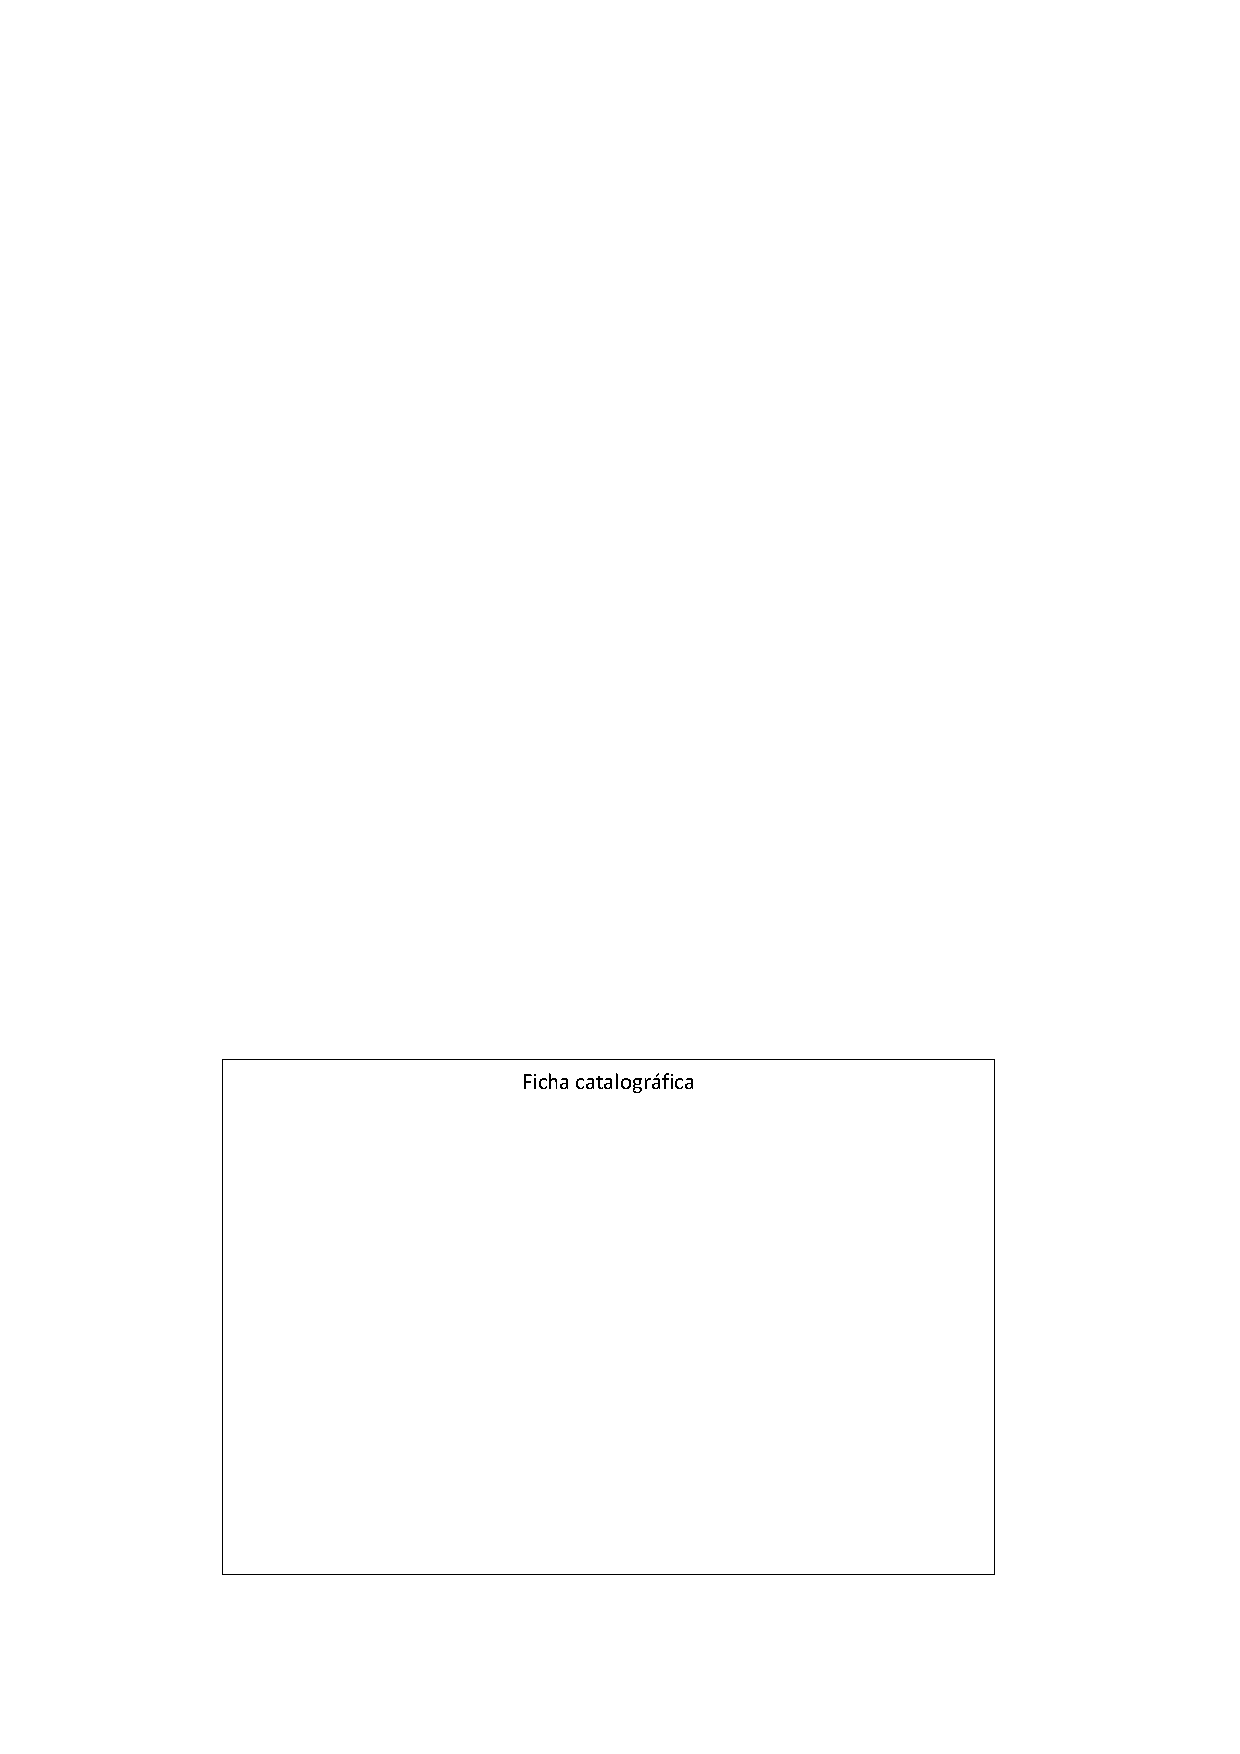
\includepdf{fig_ficha_catalografica.pdf}
%\end{fichacatalografica}

% ---
% Inserir errata
% ---
%-------------------------------------------------------------------------
% Comentário adicional do PPgSI - Informações sobre ``Errata'':
%
% Usar esta página de errata apenas em casos de excepcionais, e apenas 
% para a versão corrigida da Dissertação/Tese. Por exemplo, quando depois de
% já depositada e publicada a versão corrigida, ainda assim verifica-se
% a necessidade de alguma correção adicional.
%
% Se precisar usar esta página, busque a forma correta (o modelo correto) 
% para fazê-lo, de acordo com a norma ABNT.
%
% Não usar esta página para versão original de Dissertação/Tese.
% Não usar esta página para Qualificação.
%
%-------------------------------------------------------------------------
%\begin{errata}
%Elemento opcional para versão corrigida, depois de depositada.
%\end{errata}
% ---

% ---
% Inserir folha de aprovação
% ---

% \begin{folhadeaprovacao}
%-------------------------------------------------------------------------
% Comentário adicional do PPgSI - Informações sobre ``Folha da aprovação'':
%
% Página a ser usada apenas para Dissertação/Tese.
%
% Não usar esta página para Qualificação.
%
% Substituir ``Fulano de Tal'' pelo nome completo do autor do trabalho, com 
% apenas as iniciais em maiúsculo.
%
% Substituir ``___ de ______________ de ______'' por: 
%     - Para versão original de Dissertação/Tese: deixar em branco, pois a data 
%       pode mudar, mesmo que ela já esteja prevista.
%     - Para versão corrigida de Dissertação/Tese: usar a data em que a defesa 
%       efetivamente ocorreu.
%
% Para Tese de Doutorado: trocar "Dissertação" por "Tese".
%-------------------------------------------------------------------------
%\noindent Dissertação de autoria de Laísa Dias Brito Alves, sob o título \textbf{``\imprimirtitulo''}, apresentada à Escola de Artes, Ciências e Humanidades da Universidade de São Paulo, para obtenção do título de Mestre em Ciências pelo Programa de Pós-graduação em Sistemas de Informação, na área de concentração Metodologia e Técnicas da Computação, aprovada em \rule{0.85cm}{0.5pt} de \rule{3.5cm}{0.5pt} de \rule{1.25cm}{0.5pt} pela comissão julgadora constituída pelos doutores:

%\vspace*{3cm}

\begin{center}
%-------------------------------------------------------------------------
% Comentário adicional do PPgSI - Informações sobre ``assinaturas'':
%
% Para versão original de Dissertação/Tese: deixar em 
% branco (ou seja, assim como está abaixo), pois os membros da banca podem
% mudar, mesmo que eles já estejam previstos.
% 
% Para versão corrigida de Dissertação/Tese: usar os dados dos examinadores que 
% efetivamente participaram da defesa. 
% 
% Para versão corrigida de Dissertação/Tese: em caso de ``professora'', trocar 
% por ``Profa. Dra.'' 
% 
% Para versão corrigida de Dissertação/Tese: ao colocar os nomes dos 
% examinadores, usar seus nomes completos, exatamente conforme constam em 
% seus Currículos Lattes
% 
% Para a versão corrigida de Dissertação/Tese: remova o texto “Instituição: ”, 
% ou seja, coloque apenas/diretamente o nome da instituição, por exemplo 
% "Universidade de São Paulo" ou "Universidade Estadual de Campinas".
%
% Não abreviar os nomes das instituições.
%
% Verifique quantos membros há em sua banca, de acordo com o seu regulamento, 
% especificamente para o caso de Dissertação de Mestrado ou Tese de Doutorado, 
% e use o número correto de espaços para assinaturas.
%
%-------------------------------------------------------------------------

%\assinatura{Prof. Dr. \\ Instituição \\ Presidente}

%\assinatura{Prof. Dr. \\ Instituição}

%\assinatura{Prof. Dr. \\ Instituição}

%\assinatura{Prof. Dr. \\ Instituição}    % Incluir para bancas de tese de doutorado

%\assinatura{Prof. Dr. \\ Instituição}    % Incluir para bancas de tese de doutorado

\end{center}
  
% \end{folhadeaprovacao}
% ---

% ---
% Dedicatória
% ---
%-------------------------------------------------------------------------
% Comentário adicional do PPgSI - Informações sobre ``Dedicatória'': 
%
% Opcional para Dissertação/Tese.
% Não sugerido para Qualificação.
% 
%-------------------------------------------------------------------------
%\begin{dedicatoria}
  % \vspace*{\fill}
   %\centering
   %\noindent
   %\textit{Escreva aqui sua dedicatória, se desejar, ou remova esta página...} 
	% \vspace*{\fill}
%\end{dedicatoria}
% ---

% ---
% Agradecimentos
% ---
%-------------------------------------------------------------------------
% Comentário adicional do PPgSI - Informações sobre ``Agradecimentos'': 
%
% Opcional para Dissertação/Tese.
% Não sugerido para Qualificação.
% 
% 
% Financiamentos recebidos durante o projeto de mestrado/doutorado, vindos de qualquer 
% agência de fomento, devem ser mencionados na seção de agradecimentos da dissertação/tese. 
% Isso se aplica não apenas a bolsas de estudo, mas a qualquer tipo de financiamento, 
% tais como para apoio a participação em eventos, compra de materiais, traduções etc. 
% Especificamente para financiamento da Capes, siga as instruções contidas na portaria 
% 206, de 4/set/2018; para outras agências de fomento, procure as regras apropriadas.
%
% Portaria Capes 206, de 4/set/2018: 
% http://ppgsi.each.usp.br/arquivos/Portaria_0783227_Portaria_CAPES_DOU___206_de_2018.pdf 
%
%
%-------------------------------------------------------------------------
%\begin{agradecimentos}
%Texto de exemplo, texto de exemplo, texto de exemplo, texto de exemplo, texto de exemplo, texto de exemplo, texto de exemplo, texto de exemplo, texto de exemplo, texto de exemplo, texto de exemplo, texto de exemplo, texto de exemplo, texto de exemplo, texto de exemplo, texto de exemplo, texto de exemplo, texto de exemplo, texto de exemplo, texto de exemplo, texto de exemplo, texto de exemplo.

%Texto de exemplo, texto de exemplo, texto de exemplo, texto de exemplo, texto de exemplo, texto de exemplo, texto de exemplo, texto de exemplo, texto de exemplo, texto de exemplo, texto de exemplo, texto de exemplo, texto de exemplo, texto de exemplo, texto de exemplo, texto de exemplo, texto de exemplo, texto de exemplo, texto de exemplo, texto de exemplo, texto de exemplo, texto de exemplo.

%Texto de exemplo, texto de exemplo, texto de exemplo, texto de exemplo, texto de exemplo, texto de exemplo, texto de exemplo, texto de exemplo, texto de exemplo, texto de exemplo, texto de exemplo, texto de exemplo, texto de exemplo, texto de exemplo, texto de exemplo, texto de exemplo, texto de exemplo, texto de exemplo, texto de exemplo, texto de exemplo, texto de exemplo, texto de exemplo.

%Texto de exemplo, texto de exemplo, texto de exemplo, texto de exemplo, texto de exemplo, texto de exemplo, texto de exemplo, texto de exemplo, texto de exemplo, texto de exemplo, texto de exemplo, texto de exemplo, texto de exemplo, texto de exemplo, texto de exemplo, texto de exemplo, texto de exemplo, texto de exemplo, texto de exemplo, texto de exemplo, texto de exemplo, texto de exemplo.

%Texto de exemplo, texto de exemplo, texto de exemplo, texto de exemplo, texto de exemplo, texto de exemplo, texto de exemplo, texto de exemplo, texto de exemplo, texto de exemplo, texto de exemplo, texto de exemplo, texto de exemplo, texto de exemplo, texto de exemplo, texto de exemplo, texto de exemplo, texto de exemplo, texto de exemplo, texto de exemplo, texto de exemplo, texto de exemplo.
%\end{agradecimentos}
% ---

% ---
% Epígrafe
% ---
%-------------------------------------------------------------------------
% Comentário adicional do PPgSI - Informações sobre ``Epígrafe'': 
%
% Opcional para Dissertação/Tese.
% Não sugerido para Qualificação.
% 
%-------------------------------------------------------------------------
%\begin{epigrafe}
   % \vspace*{\fill}
	%\begin{flushright}
		%\textit{``Escreva aqui uma epígrafe, se desejar, ou remova esta página...''\\
		%(Autor da epígrafe)}
	%\end{flushright}
%\end{epigrafe}
% ---

% ---
% RESUMOS
% ---

% resumo em português
%\setlength{\absparsep}{18pt} % ajusta o espaçamento dos parágrafos do resumo
%\begin{resumo}

%-------------------------------------------------------------------------
% Comentário adicional do PPgSI - Informações sobre ``referência'':
% 
% Troque os seguintes campos pelos dados de sua Dissertação/Tese (mantendo a 
% formatação e pontuação):
%   - SOBRENOME
%   - Nome1
%   - Nome2
%   - Nome3
%   - Título do trabalho: subtítulo do trabalho
%   - AnoDeDefesa
%
% Mantenha todas as demais informações exatamente como estão.
% 
% [Não usar essas informações de ``referência'' para Qualificação]
%
% Para Tese de Doutorado: trocar "Dissertação (Mestrado em Ciências)" por "Tese (Doutorado em Ciências)".
%-------------------------------------------------------------------------
%\begin{flushleft}
%ALVES, Laísa Dias Brito. \textbf{Título do trabalho}: subtítulo do trabalho. \imprimirdata. \pageref{LastPage} f. Dissertação (Mestrado em Ciências) – Escola de Artes, Ciências e Humanidades, Universidade de São Paulo, São Paulo, 2026.
%\end{flushleft}

%Escreva aqui o texto do seu resumo... (redigido em parágrafo único, no máximo em uma página, contendo no ``máximo 500 palavras'', e apresentando um resumo de todos o seu trabalho, incluindo objetivos, metodologia, resultados e conclusões; não inclua apenas a contextualização até chegar nos objetivos, é importante fazer um resumo de todos os capítulos do texto, até chegar à conclusão). Texto de exemplo, texto de exemplo, texto de exemplo, texto de exemplo, texto de exemplo, texto de exemplo, texto de exemplo, texto de exemplo, texto de exemplo, texto de exemplo, texto de exemplo, texto de exemplo, texto de exemplo, texto de exemplo, texto de exemplo, texto de exemplo, texto de exemplo, texto de exemplo, texto de exemplo, texto de exemplo, texto de exemplo, texto de exemplo.

%Palavras-chaves: Interação Humano-Dados. Agência. Dados Pessoais. etc.
%\end{resumo}

% resumo em inglês
%-------------------------------------------------------------------------
% Comentário adicional do PPgSI - Informações sobre ``resumo em inglês''
% 
% Caso a Qualificação ou a Dissertação/Tese inteira seja elaborada no idioma inglês, 
% então o ``Abstract'' vem antes do ``Resumo''.
% 
%-------------------------------------------------------------------------
%\begin{resumo}[Abstract]
%\begin{otherlanguage*}{english}

%-------------------------------------------------------------------------
% Comentário adicional do PPgSI - Informações sobre ``referência em inglês''
% 
% Troque os seguintes campos pelos dados de sua Dissertação/Tese (mantendo a 
% formatação e pontuação):
%     - SURNAME
%     - FirstName1
%     - MiddleName1
%     - MiddleName2
%     - Work title: work subtitle
%     - DefenseYear (Ano de Defesa)
%
% Mantenha todas as demais informações exatamente como estão.
%
% [Não usar essas informações de ``referência'' para Qualificação]
%
%-------------------------------------------------------------------------
\begin{flushleft}
%SURNAME, FirstName MiddleName1 MiddleName2. \textbf{Work title}: work subtitle. \imprimirdata. \pageref{LastPage} p. Dissertation (Master of Science) – School of Arts, Sciences and Humanities, University of São Paulo, São Paulo, DefenseYear. 
\end{flushleft}

%Write here the English version of your ``Resumo''. Example text, example text, example text, example text, example text, example text, example text, example text, example text, example text, example text, example text, example text, example text, example text, example text, example text, example text, example text, example text, example text, example text, example text, example text, example text, example text, example text, example text, example text, example text, example text, example text, example text, example text, example text, example text, example text, example text, example text, example text, example text, example text, example text, example text, example text, example text, example text.

%Keywords: Keyword1. Keyword2. Keyword3. etc.
%\end{otherlanguage*}
%\end{resumo}

% ---
% ---
% inserir lista de figuras
% ---
%\pdfbookmark[0]{\listfigurename}{lof}
%\listoffigures*
%\cleardoublepage
% ---

% ---
% inserir lista de algoritmos
% ---
%\pdfbookmark[0]{\listalgorithmname}{loa}
%\listofalgorithms
%\cleardoublepage

% ---
% inserir lista de quadros
% ---
%\pdfbookmark[0]{\listofquadrosname}{loq}
%\listofquadros*
%\cleardoublepage


% ---
% inserir lista de tabelas
% ---
%\pdfbookmark[0]{\listtablename}{lot}
%\listoftables*
%\cleardoublepage
% ---

% ---
% inserir lista de abreviaturas e siglas
% ---
%-------------------------------------------------------------------------
% Comentário adicional do PPgSI - Informações sobre ``Lista de abreviaturas 
% e siglas'': 
%
% Opcional.
% Uma vez que se deseja usar, é necessário manter padrão e consistência no
% trabalho inteiro.
% Se usar: inserir em ordem alfabética.
%
%-------------------------------------------------------------------------
%\begin{siglas}
 % \item[Sigla/abreviatura 1] Definição da sigla ou da abreviatura por extenso
 % \item[Sigla/abreviatura 2] Definição da sigla ou da abreviatura por extenso
  %\item[Sigla/abreviatura 3] Definição da sigla ou da abreviatura por extenso
 % \item[Sigla/abreviatura 4] Definição da sigla ou da abreviatura por extenso
  %\item[Sigla/abreviatura 5] Definição da sigla ou da abreviatura por extenso
 % \item[Sigla/abreviatura 6] Definição da sigla ou da abreviatura por extenso
  %\item[Sigla/abreviatura 7] Definição da sigla ou da abreviatura por extenso
 % \item[Sigla/abreviatura 8] Definição da sigla ou da abreviatura por extenso
  %\item[Sigla/abreviatura 9] Definição da sigla ou da abreviatura por extenso
  %\item[Sigla/abreviatura 10] Definição da sigla ou da abreviatura por extenso
%\end{siglas}
% ---

% ---
% inserir lista de símbolos
% ---
%-------------------------------------------------------------------------
% Comentário adicional do PPgSI - Informações sobre ``Lista de símbolos'': 
%
% Opcional.
% Uma vez que se deseja usar, é necessário manter padrão e consistência no
% trabalho inteiro.
% Se usar: inserir na ordem em que aparece no texto.
% 
%-------------------------------------------------------------------------
%\begin{simbolos}
 % \item[$ \Gamma $] Letra grega Gama
 % \item[$ \Lambda $] Lambda
 % \item[$ \zeta $] Letra grega minúscula zeta
  %\item[$ \in $] Pertence
%\end{simbolos}
% ---

% ---
% inserir o sumario
% ---
\pdfbookmark[0]{\contentsname}{toc}
\tableofcontents*
\cleardoublepage
% ---



% ----------------------------------------------------------
% ELEMENTOS TEXTUAIS
% ----------------------------------------------------------
\textual



%-------------------------------------------------------------------------
% Comentário adicional do PPgSI - Informações sobre ``títulos de seções''
% 
% Para todos os títulos (seções, subseções, tabelas, ilustrações, etc.):
%
% Em maiúscula apenas a primeira letra da sentença (do título), exceto 
% nomes próprios, geográficos, institucionais ou Programas ou Projetos ou
% siglas, os quais podem ter letras em maiúscula também.
%
%-------------------------------------------------------------------------
\chapter{Introdução}

    O século XXI tem testemunhado uma rápida urbanização, com projeções da ONU indicando que mais de 60\% da população global viverá em cidades\footnote{https://brasil.un.org/pt-br/188520-onu-habitat-população-mundial-será-68-urbana-até-2050}, impulsionando a busca por soluções inteligentes e sustentáveis. Em resposta a essa demanda por soluções urbanas  a Cidades Inteligentes (\textit{Smart Cities})  têm se tornado tarefa prioritária para a comunidade científica, e também na indústria e na esfera política \cite{EREMIA201712}. As \textit{Smart Cities} utilizam tecnologias como IoT e Urbanismo de Plataforma—com smartphones atuando como sensores—para otimizar serviços urbanos, mas enfrentam desafios críticos em privacidade e segurança devido à coleta massiva de dados, muitas vezes sem transparência ou controle efetivo pelos cidadãos \cite{streitz2019beyond}. Diante disso, o paradigma da Interação humano-dados (IHD) surge como uma abordagem centrada no usuário, defendendo transparência, agência e negociabilidade para tentar reequilibrar a relação entre indivíduos e sistemas de dados, ao possibilitar o usuários usufruir dos benefícios urbanos sem comprometer direitos fundamentais \cite{mortier2015humandatainteractionhumanface}.

    Apesar do potencial da IHD, sua aplicação ainda enfrenta desafios significativos, especialmente no que diz respeito à legibilidade dos dados, agência do usuário e adaptação a contextos socioculturais diversos \cite{VICTORELLI2020Understanding}. Pesquisas (\ref{SinteseArtigos}) apontam lacunas importantes, como a dificuldade de engajamento dos usuários no design de sistemas e a falta de clareza em contratos de uso de dados, problema evidenciado em estudos com populações vulneráveis, que frequentemente concordam com termos sem plena compreensão. Além disso, fatores contextuais, como diferenças culturais e ambiguidades interpretativas, influenciam diretamente como os dados são gerenciados e compartilhados, exigindo abordagens mais inclusivas e adaptáveis para que a interação humano-dado seja mais clara e ética.

    Diante desses desafios, esta proposta de pesquisa investiga a gestão de dados pessoais em aplicações urbanas de cidades inteligentes, tomando São Paulo como estudo de caso. Partindo dos princípios da IHD (legibilidade, agência e negociabilidade), o estudo busca: (1) analisar como esses fundamentos se materializam na prática em soluções tecnológicas urbanas, e (2) compreender a percepção e o nível de controle que os cidadãos têm sobre seus dados nessas plataformas.

    Inicialmente foi realizada uma Revisão Sistemática da Literatura (RSL) seguindo o protocolo de Kitchenham para mapear o estado da arte sobre os princípios da IHD (legibilidade, agência e negociabilidade), abrangendo bases como Scopus, Web of Science e IEEE Xplore nos últimos 10 anos, com análise bibliométrica e de conteúdo; (2) Estudo Empírico com análise técnica de aplicações urbanas em São Paulo, incluindo mapeamento da jornada do usuário (fluxos de interação, pontos de coleta de dados, mecanismos de consentimento e usabilidade) e avaliação do ciclo de vida dos dados; e (3) Pesquisa de Campo qualitativa com usuários paulistanos, mediante questionário semiestruturado (presencial e online) sobre percepção de uso de dados, conhecimento de políticas de privacidade, controle percebido e preocupações com segurança, seguido de análise de conteúdo das respostas.

    %Para avaliar sistematicamente os resultados desta tripla abordagem, o estudo criará e implementará um framework misto de avaliação, articulando análises intrínseca e extrínseca. A dimensão intrínseca examinará as aplicações através de heurísticas adaptadas de HDI (legibilidade: clareza de políticas e metáforas visuais; agência: granularidade de configurações e revogabilidade; negociabilidade: flexibilidade nos termos), utilizando uma escala de 0 a 3 para pontuação comparativa, enquanto a dimensão extrínseca pretende capturar a percepção dos usuários por meio de entrevistas semiestruturadas (N=200, estratificadas por região e idade) sobre compreensão de termos e preocupações com privacidade, complementadas por \textit{survey} quantitativo (N=200) adaptado da Privacy Concerns Scale, focado na percepção sobre coleta de dados por sensores urbanos.

    %A abordagem se justifica pelo crescimento acelerado das smart cities e pela coleta massiva de dados via dispositivos móveis - que, embora tragam eficiência operacional, intensificam riscos à privacidade. Ao focar no contexto específico de uma metrópole latino-americana, a pesquisa visa contribuir para o desenvolvimento de frameworks adaptados às realidades regionais, identificando lacunas entre os princípios da HDI e sua implementação concreta na governança de dados urbanos.

    %Esta pesquisa investiga os desafios da gestão de dados pessoais no contexto das cidades inteligentes, com foco em aplicações urbanas da cidade de São Paulo. Partindo do paradigma da Human-Data Interaction (IHD) - que propõe os princípios de legibilidade, agência e negociabilidade para equilibrar a utilidade dos dados e proteção da privacidade -, o estudo analisará como essas premissas teóricas se manifestam na prática em soluções tecnológicas urbanas. A investigação busca compreender especialmente a percepção e o grau de controle que os cidadãos paulistanos têm sobre seus dados pessoais nestas aplicações.

    %O trabalho se justifica diante do crescimento acelerado das cidades inteligentes e da coleta massiva de dados urbanos através de dispositivos como smartphones, que, embora tragam benefícios operacionais, apresentam sérios riscos à privacidade individual. Ao examinar a implementação dos princípios da IHD no contexto específico de uma metrópole latino-americana, a pesquisa pretende contribuir para o desenvolvimento de frameworks mais adequados às realidades socioculturais da região, identificando lacunas entre a teoria e a prática na governança de dados urbanos.


% \section{Tema}
%  \section{Motivação}

%\section{Objetivos}

% \section{Método}

 %\chapter{Fundamentação Teórica}

\chapter{Trabalhos Relacionados}

    Este capítulo introduz a fundamentação teórica e os delineamentos da Revisão Sistemática da Literatura (RSL) conduzida para mapear o estado da arte da Interação Humano-Dados (IHD) em contextos urbanos sociotécnicos. O levantamento, embasado nas diretrizes de \citeonline{KITCHENHAM2013} e alinhado às recomendações do protocolo PRISMA, tem como objetivo consolidar o referencial necessário para a etapa empírica desta dissertação, focada na análise de aplicativos de amplo uso na cidade de São Paulo. O rigoroso detalhamento do processo investigativo — englobando o protocolo metodológico, as questões de pesquisa, a estratégia de busca e as etapas de condução e síntese — será apresentado nas seções subsequentes.

    A adoção desse método viabiliza a síntese estruturada da literatura, permitindo articular as formulações teóricas da IHD com os desafios de suas implementações práticas. A estratégia exploratória abrangeu repositórios multidisciplinares (Scopus e Science Direct) e acervos nacionais (Portal de Periódicos CAPES, Catálogo de Teses da CAPES e BDTD-USP), utilizando descritores cruzados entre governança de dados e ecossistemas urbanos. O \textit{corpus} bibliográfico resultante engloba desde propostas de \textit{frameworks} conceituais até estudos de caso aplicados, os quais foram selecionados mediante critérios preestabelecidos, com o intuito de conferir pertinência, transparência e reprodutibilidade ao referencial analisado.
    
  

\section{Objetivo}

    A RSL tem como objetivo principal mapear o estado da arte e estabelecer o arcabouço teórico em torno da Interação Humano-Dados (IHD), com especial atenção aos seus princípios fundamentais. Secundariamente, o levantamento busca investigar a evolução do tema na última década, identificando lacunas na literatura, tendências teóricas e práticas metodológicas recorrentes na área.

    Conduzida sob as diretrizes de \citeonline{KITCHENHAM2013}, esta revisão cumpre também um propósito instrumental fundamental para a pesquisa: fornecer o embasamento metodológico e conceitual para as etapas empíricas subsequentes. Dessa forma, os achados da RSL visam subsidiar tanto a estruturação da análise técnica de algumas aplicações urbanas de São Paulo quanto a elaboração do questionário qualitativo, buscando alinhar a investigação de campo e a avaliação dos mecanismos de dados ao panorama científico atual.


    %A RSL tem como objetivo principal mapear o estado da arte dos princípios de IHD, conforme estabelecido no protocolo de pesquisa. Como objetivo secundário, pretende-se identificar a exploração do conceito e princípios da IHD nos últimos dez anos, lacunas de conhecimento, tendências teóricas, além de práticas mais recorrentes da área, a fim de obter uma base para orientar as etapas subsequentes da pesquisa. Essa revisão procura contextualizar o estudo dentro do panorama científico atual, mas também contribui na seleção dos princípios de IHD a serem analisados nas aplicações urbanas de São Paulo, seguindo as melhores práticas para revisões sistemáticas conforme \citeonline{KITCHENHAM2013}.

 
    \section{Protocolo de Revisão Sistemática}

    O escopo metodológico delineado neste protocolo estrutura-se em frentes complementares de investigação sobre a Interação Humano-Dados (IHD). O levantamento busca compreender a evolução conceitual e prática da área na última década, mapeando tanto as estratégias que antecederam a adoção formal da IHD quanto as eventuais divergências entre proposições teóricas e implementações reais. 

    De forma complementar, no cenário das cidades inteligentes (\textit{Smart Cities}), o foco direciona-se não apenas à articulação dos princípios basilares de legibilidade, agência e negociabilidade, mas também abrange aspectos técnicos de transparência e o ciclo de vida dos dados nas aplicações. Por fim, a revisão explora as dinâmicas associadas ao letramento digital, aos métodos de avaliação de eficácia e à experiência dos cidadãos diante da coleta de dados pessoais, buscando compreender como fatores socioculturais influenciam a capacidade dos usuários de assimilar e gerenciar suas próprias informações.
    
    %Para operacionalizar os objetivos propostos, esta seção detalha o protocolo estruturado para a condução da pesquisa bibliográfica. Alinhado às diretrizes de \citeonline{KITCHENHAM2013}, o planejamento da revisão foi segmentado em etapas sequenciais, com o intuito de promover o rigor analítico e favorecer a reprodutibilidade de todo o processo investigativo.

    %O escopo metodológico delineado neste protocolo volta-se especificamente à investigação de como a literatura articula a Interação Humano-Dados (IHD) e seus princípios basilares — legibilidade, agência e negociabilidade — no desenvolvimento de aplicações urbanas. Para tanto, as subseções a seguir discriminam os componentes práticos do levantamento, abrangendo a definição das bases de dados, o recorte temporal, as questões de pesquisa, a estratégia de busca e os critérios adotados para a seleção e síntese dos estudos primários.

    %Esta seção descreve o protocolo metodológico adotado para a revisão sistemática da literatura, seguindo as diretrizes estabelecidas por \citeonline{KITCHENHAM2013}. O objetivo é mapear o estado da arte sobre a IHD em aplicativos urbanos, com foco nos princípios de legibilidade, agência e negociabilidade. Para isso, foram definidas etapas, desde a formulação das questões de pesquisa até a seleção e avaliação dos estudos, garantindo a reprodutibilidade. As subseções seguintes detalharão cada componente do protocolo, incluindo as bases de dados consultadas, os critérios de inclusão e exclusão, a estratégia de busca e os métodos de análise dos dados. Essa estrutura visa não apenas consolidar o conhecimento existente, mas também identificar lacunas e tendências relevantes para o contexto da pesquisa.

\subsection{Base de Dados}

    A estratégia de busca desta Revisão Sistemática da Literatura pautou-se na consulta a repositórios científicos diversificados, contemplando bases de dados internacionais e nacionais. No âmbito internacional, a \emph{Scopus}\footnote{https://www.scopus.com} foi selecionada como fonte principal devido ao seu escopo multidisciplinar, adequado para mapear a interseção entre a tecnologia da informação e o contexto urbano. Embora repositórios nativos e centrais para a área de IHD, como a ACM Digital Library e a IEEE Xplore, ofereçam indexação profunda em texto completo, a escolha pela Scopus justificou-se pela padronização na extração de metadados via campo \textit{TITLE-ABS-KEY}, permitindo priorizar os trabalhos de maior impacto dessas editoras, os quais são sistematicamente indexados por essa plataforma.

    Por sua vez, a integração da base \emph{Science Direct}\footnote{https://www.sciencedirect.com} atuou de maneira complementar para suprir a necessidade de buscas diretas em textos completos (\textit{full-text}). Sua escolha fundamentou-se na forte aderência de seus periódicos às áreas de sistemas de informação e ecossistemas urbanos, permitindo capturar estudos empíricos cujas discussões sobre usabilidade e governança de dados em \textit{Smart Cities} estivessem detalhadas no corpo metodológico dos trabalhos, e não apenas refletidas nos resumos.

    Considerando que a etapa empírica desta dissertação tem como foco as aplicações urbanas da cidade de São Paulo, a análise da produção científica brasileira fez-se necessária. Para o mapeamento do desenvolvimento da IHD no cenário acadêmico nacional, foram consultados o Portal de Periódicos CAPES\footnote{https://www.periodicos.capes.gov.br}, o Catálogo de Teses e Dissertações da CAPES\footnote{https://catalogodeteses.capes.gov.br} e a Biblioteca Digital de Teses e Dissertações da USP (BDTD-USP)\footnote{https://www.teses.usp.br}.
    
    %Para a revisão sistemática, esta pesquisa utilizará fontes diversificadas que incluem bases internacionais e nacionais de relevância acadêmica reconhecida. A \emph{Scopus \footnote{https://www.scopus.com}} foi selecionada como fonte principal por seu amplo escopo, indexando artigos de alto impacto de editoras como Elsevier, IEEE Xplore e ACM Digital Library, além de oferecer cobertura de periódicos internacionais.

    %Adicionalmente, serão consultadas bases especializadas como o \emph{Science Direct \footnote{https://www.sciencedirect.com}} para acesso a publicações técnicas, e o \emph{Portal de Periódicos CAPES \footnote{https://www.periodicos.capes.gov.br}} para a inclusão de produção científica nacional. Para abranger pesquisas acadêmicas brasileiras relevantes, serão utilizados os \emph{Repositórios de Teses da USP \footnote{https://www.teses.usp.br}} e da \emph{CAPES \footnote{https://catalogodeteses.capes.gov.br}}.


\subsection{Período de Publicação}


    O recorte temporal estabelecido para esta Revisão Sistemática da Literatura abrange o intervalo de 2014 a 2024. Essa delimitação justifica-se por coincidir com o período de maior visibilidade e estruturação teórica da Interação Humano-Dados (IHD). Identifica-se que, em meados da década de 2010, o tema passou a figurar com maior frequência na literatura científica, impulsionado por trabalhos pioneiros como o de \citeonline{mortier2015humandatainteractionhumanface}, considerado uma referência na proposição das bases conceituais sobre a relação entre os indivíduos e seus dados pessoais.

    A cobertura desse intervalo de dez anos viabiliza um acompanhamento cronológico consistente, partindo das primeiras formulações teóricas até as discussões recentes associadas aos princípios de legibilidade e agência. Esse horizonte temporal permite, ainda, situar a evolução da IHD de forma paralela ao próprio amadurecimento das cidades inteligentes (\textit{Smart Cities}), um cenário em que a coleta e o processamento de dados urbanos se tornaram cada vez mais complexos.

   Além disso, o período selecionado capta o impacto do surgimento de marcos regulatórios fundamentais para a privacidade. Destacam-se o Regulamento Geral sobre a Proteção de Dados (RGPD/GDPR\footnote{https://gdpr.eu/what-is-gdpr}), implementado em 2018, e a Lei Geral de Proteção de Dados Pessoais (LGPD\footnote{https://www.planalto.gov.br/ccivil\_03/\_ato2015-2018/2018/lei/l13709.htm}), em vigor no Brasil desde 2020. Por fim, estabelecer o limite da busca em 2024 busca contemplar as investigações mais atuais sobre os desafios emergentes na manipulação de informações no ambiente digital.

%O recorte temporal desta revisão sistemática abrange o período de 2014 a 2024, selecionado por representar a consolidação do campo de Interação Humano-Dados (IHD) como área de estudo distinta. Foi precisamente em meados da década de 2010 que o termo IHD emergiu na literatura acadêmica, particularmente nos trabalhos pioneiros de \citeonline{mortier2015humandatainteractionhumanface}, que estabeleceram as bases conceituais para o estudo sistemático da relação entre humanos e dados pessoais. Este período de dez anos permite acompanhar tanto a fundamentação teórica inicial quanto os desenvolvimentos recentes em tópicos como legibilidade, agência e gestão de dados pessoais, especialmente no contexto das cidades inteligentes e das novas regulamentações de proteção de dados (como a GDPR\footnote{https://gdpr.eu/what-is-gdpr}, implementada em 2018 ). A delimitação até 2024 assegura a inclusão das pesquisas mais atuais sobre os desafios emergentes na interação com dados pessoais.

\subsection{Questões de Pesquisa} \label{questoesdepesquisa}

    Esta revisão sistemática foi estruturada a partir de um conjunto hierárquico de questões, elaboradas para mapear o estado da arte da Interação Humano-Dados e identificar os desafios emergentes na área. As questões foram divididas da seguinte forma:

\textbf{Questões Principais (QP):}
\begin{itemize}
    \item[] \textbf{QP1} - Como a literatura sobre Interação Humano-Dados (IHD) evoluiu conceitual e empiricamente na última década (2014-2024)?
    \item[] \textbf{QP2} - Quais são as principais divergências ou alinhamentos entre as abordagens teóricas e as implementações práticas relatadas na literatura nesse período?
    \item[] \textbf{QP3} - Quais são as lacunas de pesquisa mais recorrentemente apontadas nos estudos primários?
    \item[] \textbf{QP4} - Quais estratégias ou abordagens precederam a adoção formal da IHD para facilitar a compreensão e a gestão de dados em aplicações?
    \item[] \textbf{QP5} - Qual é a relevância da aplicação dos princípios de IHD no ecossistema de cidades inteligentes (\textit{Smart Cities})?
\end{itemize}

\textbf{Questões Secundárias (QPS):}
\begin{itemize}
    \item[] \textbf{QPS1} - Quais métodos de avaliação (ex.: testes de usabilidade, \textit{eye-tracking}) são empregados para mensurar a eficácia da IHD?
    \item[] \textbf{QPS2} - Quais elementos em sistemas de IHD auxiliam usuários com baixo letramento digital a compreender melhor o uso de seus dados?
    \item[] \textbf{QPS3} - Quais \textit{frameworks} fundamentados em IHD foram validados ou testados por meio de estudos de caso empíricos?
    \item[] \textbf{QPS4} - De que forma fatores étnico-culturais influenciam a implementação e a apropriação das diretrizes de IHD?
\end{itemize}

    Para operacionalizar as respostas a essas questões, a condução desta revisão pautou-se em um protocolo estruturado em cinco dimensões. Essa abordagem permitiu não apenas sintetizar o referencial teórico, mas também estabelecer conexões sólidas entre os aspectos conceituais e práticos da IHD, servindo como alicerce metodológico para as etapas empíricas desta pesquisa. Os componentes-chave do levantamento foram definidos da seguinte maneira:

\begin{itemize}
    \item[]\textbf{Intervenção:} O mapeamento do escopo conceitual da IHD, contemplando seus princípios teóricos fundamentais, as metodologias de mensuração aplicáveis e as principais lacunas científicas apontadas pela literatura;
    \item[] \textbf{Controle:} A seleção pautou-se em critérios sistemáticos, priorizando estudos que propusessem (re)formulações de princípios de IHD, apresentassem aplicações práticas ou discutissem métodos de avaliação nesse contexto;
    \item[] \textbf{População:} Trabalhos acadêmicos e estudos empíricos que demonstrassem aplicações concretas ou discussões teóricas sobre a IHD em contextos diversificados;
    \item[] \textbf{Resultados:} A consolidação das evidências sobre métodos e técnicas empregados, culminando em um panorama abrangente das tendências e carências da área;
    \item[] \textbf{Aplicação:} A geração de subsídios teóricos e práticos destinados a pesquisadores de IHD e Interação Humano-Computador (IHC), bem como a profissionais interessados na adoção e avaliação desses princípios no desenvolvimento de sistemas.
\end{itemize}

    \subsection{Estratégia de Busca}
    \label{estrategiaDeBusca}

    Esta subseção descreve a estratégia metodológica empregada para identificar e selecionar os estudos relevantes sobre Interação Humano-Dados (IHD) em aplicações urbanas. Para promover a abrangência pertinente, a investigação fundamentou-se na formulação de equações de busca específicas, aliadas a critérios sistemáticos de filtragem. Essa estruturação tem o intuito de favorecer a seleção de um referencial de alta qualidade metodológica e representativo do estado da arte no tema investigado.

    Para operacionalizar esse levantamento, o processo envolveu a definição de palavras-chave, a configuração dos repositórios científicos e a aplicação de recortes temporais e linguísticos. A partir dessa base, detalham-se a seguir os componentes essenciais aplicados nesta etapa: a \textit{string} de busca, os tipos de documentos elegíveis, os idiomas prioritários e os critérios de inclusão e exclusão.

   \subsubsection{\textit{String} de Busca}

    Considerando a relativa recência das pesquisas sobre IHD, optou-se pela adoção da expressão explícita ``Human-Data Interaction'' como termo central da busca. Na base principal selecionada (\emph{Scopus}), essa \textit{string} foi aplicada aos campos de título, resumo e palavras-chave (\textit{TITLE-ABS-KEY}), com o objetivo de recuperar um conjunto de artigos estritamente alinhado à temática.

    O processo de triagem seguiu uma lógica sistemática: a busca foi parametrizada para integrar requisitos temáticos e cronológicos logo em sua primeira execução, viabilizando a aplicação fluida e estruturada das etapas subsequentes de inclusão, exclusão e avaliação de qualidade. Dessa forma, buscou-se favorecer a identificação das contribuições mais atuais e metodologicamente robustas do campo.

    Para equilibrar o alcance da pesquisa com a precisão dos resultados, o recorte temporal de 2014 a 2024 foi implementado diretamente na configuração das plataformas de busca. Esse filtro operacionalizou a delimitação justificada anteriormente, varrendo a literatura desde os trabalhos pioneiros que consolidaram o conceito até seus desdobramentos mais recentes.

    \subsubsection{Tipo dos Artigos}

    Para compor o \textit{corpus} desta revisão, foram considerados elegíveis trabalhos acadêmicos que transitem entre a fundamentação teórica e a investigação prática. No escopo conceitual, foram privilegiados estudos voltados ao estabelecimento de definições, \textit{frameworks}, propostas de diretrizes e ensaios de posicionamento (\textit{position papers}). No escopo empírico e experimental, foram contempladas pesquisas que relatam a criação de protótipos, provas de conceito, experimentos controlados e análises de soluções aplicadas ao ambiente urbano.

    Adicionalmente, consideraram-se pertinentes os estudos de natureza metodológica e as investigações centradas no usuário. Nessa categoria, incluíram-se pesquisas de levantamento (\textit{surveys}), estudos de caso, pesquisa-ação e métodos qualitativos ou observacionais que busquem mensurar a usabilidade, a eficácia e o impacto na compreensão dos sistemas de IHD por parte dos cidadãos.

   As pesquisas secundárias, representadas por revisões sistemáticas e mapeamentos da literatura, também foram admitidas no levantamento. Nesse eixo, conferiu-se destaque aos trabalhos que abordavam tópicos correlatos, como visualização de informações e experiência do usuário em ferramentas analíticas.

    Por fim, como critério de alinhamento temático, priorizou-se a seleção de pesquisas que explorem a IHD aplicada a contextos urbanos específicos. Nesse cenário, destacaram-se os trabalhos voltados ao ecossistema de cidades inteligentes (\textit{Smart Cities}), à governança de dados e aos mecanismos de participação cidadã mediados por essas tecnologias.
    
    %Foram considerados elegíveis os trabalhos acadêmicos desde  contribuições teóricas que estabelecem definições, frameworks e princípios fundamentais da área, até estudos de caso concretos que documentam implementações reais em soluções urbanas - como aplicativos, painéis de controle e plataformas de análise de dados.

    %Foram incluídos também artigos metodológicos que propõem ou avaliam técnicas para mensurar usabilidade, eficácia e impacto no aprendizado em sistemas de IHD. Revisões sistemáticas e mapeamentos do estado da arte são igualmente valiosos para nosso estudo, especialmente aqueles que abordam tópicos correlatos como visualização de dados e experiência do usuário em ferramentas analíticas. Por fim, daremos atenção especial às pesquisas que exploram aplicações específicas em contextos urbanos---incluindo cidades inteligentes, governança de dados e mecanismos de participação cidadã mediados por tecnologias de IHD.

    %Para obter o maior número de estudos possíveis para o recorte escolhido serão considerados aptos os artigos:
    %\begin{itemize}
    %\item Artigos teóricos (Definições, frameworks e princípios de IHD);
    %\item Estudos de Caso Aplicados (Implementações reais de IHD em soluções urbanas - apps, dashboards, plataformas);
    %\item Artigos Metodológicos (Métodos para mensurar usabilidade, aprendizado ou eficácia em IHD);
    %\item Revisões Sistemáticas ou Mapeamentos(ínteses do estado da arte em IHD ou tópicos correlatos - visualização de dados, UX em ferramentas analíticas);
    %\item Artigos sobre Contextos Urbanos (Aplicações específicas em cidades inteligentes, governança de dados ou participação cidadã.);
    %\end{itemize}

   \subsubsection{Idioma dos Artigos}

    A IHD consolida-se como um campo de pesquisa em expansão, embora ainda apresente lacunas relativas à sua diversidade multicultural. Diante desse panorama, a estratégia de busca optou por não aplicar filtros restritivos de idioma diretamente nas bases de dados. Contudo, considerando a predominância da língua inglesa na produção científica acadêmica e o alinhamento empírico desta dissertação com o cenário urbano brasileiro, priorizaram-se os trabalhos redigidos em inglês e português durante a etapa de seleção.

    \subsubsection{Critérios de Inclusão e Exclusão}

    Com o propósito de delimitar um \textit{corpus} pertinente à temática investigada, estabeleceram-se critérios sistemáticos de inclusão e exclusão. Esses parâmetros foram delineados com base no escopo da dissertação e no objetivo de mapear as contribuições mais significativas para o campo da IHD.

    A triagem dos estudos ponderou aspectos tanto conceituais quanto metodológicos, visando que a síntese final refletisse de forma abrangente o estado da arte na área. Dessa forma, as diretrizes adotadas buscaram equilibrar a abrangência da busca com a especificidade necessária para responder de maneira precisa às questões de pesquisa propostas.

    \subsubsection{Critérios de inclusão}\label{crit:Inclu}
    
    Os critérios de inclusão foram estabelecidos com o intuito de contemplar tanto os desenvolvimentos teóricos quanto as aplicações práticas da área. A seleção privilegiou trabalhos que oferecessem contribuições substanciais por meio de avanços conceituais, metodológicos ou empíricos. Além disso, definiram-se parâmetros focados no rigor acadêmico, no alinhamento ao contexto urbano sociotécnico e na pertinência temporal das publicações, visando delinear um panorama representativo e fundamentado do estado da arte em IHD.
    
    Os estudos elegíveis precisaram atender a pelo menos um dos seguintes critérios temáticos ou metodológicos, somados aos critérios obrigatórios de qualidade e temporalidade:

\begin{itemize}
\item[] \textbf{CI1} - Trabalhos que proponham, definam ou aprimorem princípios teóricos e fundamentais da IHD;
\item[] \textbf{CI2} - Estudos que apresentem a formulação ou aplicação prática de \textit{frameworks} baseados nesses princípios;
\item[] \textbf{CI3} - Pesquisas focadas no desenvolvimento, aplicação ou validação de métricas e métodos de avaliação em sistemas de IHD;
\item[] \textbf{CI4} - Artigos que relatem resultados empíricos (qualitativos ou quantitativos) acerca da eficácia e da usabilidade de soluções ou \textit{frameworks} de IHD;
\item[] \textbf{CI5} - Modelos teóricos sustentados e validados por evidências concretas, tais como estudos de caso e experimentos controlados;
\item[] \textbf{CI6} - Revisões sistemáticas e mapeamentos da literatura que ofereçam contribuições originais ou consolidações teóricas relevantes para a área;
\item[] \textbf{CI7} - Publicações submetidas a processo de revisão por pares (\textit{peer-review}), incluindo anais de conferências indexadas e periódicos acadêmicos;
\item[] \textbf{CI8} - Trabalhos publicados no período estabelecido para o levantamento metodológico, compreendendo os anos de 2014 a 2024.
\end{itemize}

    A aplicação sistemática desses critérios de inclusão viabilizou a conformação de um corpus inicial qualificado. Contudo, para assegurar a aderência estrita dos trabalhos ao escopo analítico desta revisão e mitigar a presença de falsos positivos ou pesquisas apenas tangenciais à temática abordada, a triagem exigiu uma etapa complementar de refinamento. Para essa finalidade, definiram-se os critérios de exclusão, detalhados na subseção a seguir.
    
\subsubsection{Critérios de Exclusão}
\label{crit:exclu}

    Conforme antecipado, os critérios de exclusão atuaram como uma camada de refinamento para assegurar a estrita aderência da amostra ao escopo da pesquisa. Esses parâmetros foram estruturados em eixos centrais que consideram a reprodutibilidade metodológica, a centralidade temática na Interação Humano-Dados (IHD), a acessibilidade ao conteúdo integral e a originalidade dos registros. Dessa forma, foram removidos do \textit{corpus} os estudos que se enquadraram em pelo menos uma das seguintes condições:

\begin{itemize}
    \item[] \textbf{CE1} - Trabalhos com metodologia não replicável ou que não apresentem uma descrição clara e rigorosa dos procedimentos adotados;
    \item[] \textbf{CE2} - Artigos que citem a IHD de maneira apenas tangencial ou superficial, sem aprofundamento em seus princípios, \textit{frameworks} ou métricas;
    \item[] \textbf{CE3} - Estudos focados exclusivamente em visualização de dados, mas que não abordem o componente ativo de interação humana;
    \item[] \textbf{CE4} - Pesquisas que empreguem a sigla ou o termo atrelado à IHD em contextos não correlatos (como interfaces estritas de \textit{hardware} ou interações em baixo nível computacional);
    \item[] \textbf{CE5} - Trabalhos publicados em período anterior a 2014, situando-se fora do recorte temporal delimitado para a revisão;
    \item[] \textbf{CE6} - Documentos disponibilizados apenas em formato de resumo expandido, \textit{abstract} ou cujos textos completos encontravam-se indisponíveis;
    \item[] \textbf{CE7} - Documentos com texto integral indisponível gratuitamente (restritos a \textit{paywalls} ou bibliotecas pagas);
    \item[] \textbf{CE8} - Artigos voltados estritamente à área médica ou clínica, afastando-se do escopo sociotécnico e urbano estabelecido por esta investigação;
    \item[] \textbf{CE9} - Registros duplicados nas bases de dados, sendo contabilizada para análise apenas a versão mais completa, recente ou indexada na base prioritária.
\end{itemize}

    A triagem fundamentada na aplicação conjunta dos critérios de inclusão e exclusão permitiu refinar o levantamento inicial, delimitando um corpus final estritamente alinhado aos objetivos desta investigação. Por meio desse filtro bidirecional, buscou-se mitigar vieses de seleção e afastar abordagens meramente tangenciais, consolidando a base de evidências que fundamenta as análises e as discussões desenvolvidas nas etapas subsequentes desta pesquisa.


  \subsubsection{Critérios de Avaliação de Qualidade}
\label{crit:quali}

    Os estudos retidos após a aplicação dos filtros de inclusão e exclusão foram submetidos a uma avaliação de qualidade e relevância temática. Para classificar o grau de aderência e o peso metodológico dos trabalhos no escopo da pesquisa, bem como facilitar a rastreabilidade na planilha de síntese dos resultados, estabeleceu-se o seguinte sistema de identificação e pontuação:

\begin{itemize}
    \item[] \textbf{CQ1 (Pontuação -1):} Artigos que, após leitura flutuante, revelaram-se sem revisão por pares confirmada (atuando como dupla verificação de exclusão);
    \item[] \textbf{CQ2 (Pontuação 0):} Artigos sem contribuição estrutural ou metodológica relevante para o núcleo da pesquisa;
    \item[] \textbf{CQ3 (Pontuação 1):} Artigos que abordem apenas um dos eixos temáticos principais da investigação;
    \item[] \textbf{CQ4 (Pontuação 2):} Artigos que articulem simultaneamente dois dos eixos temáticos principais da investigação;
    \item[] \textbf{CQ5 (Pontuação 3):} Artigos que integrem de forma holística três ou mais eixos temáticos principais da investigação.
\end{itemize}

    A partir da aplicação dessa métrica, os trabalhos associados aos identificadores \textbf{CQ4} e \textbf{CQ5} (que atingiram 2 e 3 pontos, respectivamente) receberam prioridade para a etapa de extração integral de dados, compondo o núcleo principal de análise da revisão sistemática da literatura.
   
   %Os estudos selecionados mediante a aplicação dos critérios de inclusão e exclusão serão posteriormente avaliados quanto à sua qualidade metodológica, conforme o seguinte sistema de pontuação:

   
%(a) Artigos sem revisão por pares: -1

%(b) Artigos sem contribuição relevante para a pesquisa: 0

%(c) Artigos que contenham apenas um dos temas principais da pesquisa: 1

%(d) Artigos que contenham dois dos temas principais da pesquisa: 2 

%(e) Artigos que tratem 3 ou mais temas principais da pesquisa: 3

    %Os artigos que atingirem as pontuações mais elevadas (2 e 3 pontos) terão prioridade para análise integral e posterior inclusão na revisão sistemática da literatura.


    \subsection{Procedimento de seleção de estudos}
    \label{procedimentoSelecao}

    O procedimento de seleção dos estudos foi estruturado em quatro etapas sequenciais de filtragem, com o propósito de favorecer a composição de um \textit{corpus} robusto e alinhado aos objetivos desta investigação:

\begin{itemize}
    \item[] \textbf{Primeira etapa (Triagem preliminar):} Realizou-se a análise sistemática dos títulos e dos resumos de todas as publicações recuperadas, com o intuito de avaliar a pertinência temática inicial frente ao escopo delimitado;
    \item[] \textbf{Segunda etapa (Depuração):} Executou-se a identificação e a remoção dos registros duplicados, tanto de forma interna em cada repositório quanto no cruzamento entre as bases de dados selecionadas;
    \item[] \textbf{Terceira etapa (Avaliação integral):} Procedeu-se à leitura completa dos artigos remanescentes da fase anterior, aplicando-se rigorosamente os critérios de inclusão e exclusão delineados no protocolo;
    \item[] \textbf{Quarta etapa (Qualificação e extração):} Conduziu-se a avaliação dos trabalhos elegíveis por meio do sistema de critérios de qualidade (\textit{CQ}), direcionando a extração definitiva de dados ao atendimento das questões de pesquisa principais (\textit{QP}) e subquestões (\textit{QPS}).
\end{itemize}

    \subsection{Estratégia de síntese dos dados}

    A etapa de extração e síntese de dados transcendeu a simples compilação de informações, configurando-se como um processo analítico de categorização do \textit{corpus} final. Com o intuito de estruturar o conhecimento levantado, a leitura documental focou em mapear criticamente as soluções metodológicas empregadas, os padrões de interação propostos e, sobretudo, as lacunas científicas diagnosticadas pelos autores. Esse procedimento sistemático permitiu organizar os achados dispersos na literatura em um formato passível de cruzamento e avaliação objetiva.

    Os dados extraídos foram submetidos a uma análise qualitativa inicial e organizados em uma matriz comparativa. Essa consolidação foi estruturada em cinco eixos centrais para facilitar o cruzamento das informações:

\begin{itemize}
    \item[] \textbf{Eixo 1:} Identificação e caracterização dos estudos selecionados;
    \item[] \textbf{Eixo 2:} Escopo de aplicação e princípios de IHD abordados;
    \item[] \textbf{Eixo 3:} Métodos de avaliação e métricas específicas utilizadas;
    \item[] \textbf{Eixo 4:} Técnicas propostas para garantir a intuitividade dos sistemas;
    \item[] \textbf{Eixo 5:} Lacunas metodológicas ou conceituais identificadas em cada pesquisa.
\end{itemize}

    A partir dessa estruturação, foi possível evidenciar convergências teóricas e disparidades metodológicas, fornecendo respostas significativas aos objetivos do estudo. Complementarmente, procedeu-se ao mapeamento das abordagens adotadas para mensurar a eficácia e a usabilidade das soluções propostas. A extração destacou a predominância de métodos qualitativos e mistos --- englobando desde \textit{workshops} de \textit{co-design} e entrevistas até o emprego de escalas psicométricas e rastreamento ocular (\textit{eye-tracking}) ---, viabilizando uma compreensão crítica sobre como o desempenho e a aceitação dos sistemas têm sido avaliados na área.

    A adoção dessa abordagem híbrida revelou-se fundamental para a compreensão consolidada do estado da arte na área. Desse modo, o estudo articulou avaliações intrínsecas (técnico-metodológicas) e extrínsecas (contextuais) para examinar a implementação dos princípios de IHD em aplicações urbanas, com especial direcionamento ao cenário de São Paulo. O processo de síntese foi delineado para responder aos três objetivos específicos da pesquisa, conforme detalhado adiante.


    
    %Na fase de análise documental, cada estudo selecionado passará por um processo sistemático de extração de dados, com foco em compreender sua abordagem sobre Interação Humano-Dados. Esta análise buscará identificar o escopo específico de aplicação de IHD adotado pela pesquisa, os princípios teóricos que fundamentam sua proposta, bem como os métodos de avaliação utilizados para validar os resultados. Serão particularmente examinadas as técnicas de interação consideradas mais intuitivas pelos autores, ao mesmo tempo em que se registrarão as lacunas metodológicas ou conceituais deixadas pelo estudo - elementos essenciais para um mapeamento crítico do campo.

    %Os dados coletados serão submetidos a uma análise qualitativa inicial, sintetizada em uma tabela comparativa estruturada em cinco eixos: (a) identificação dos estudos selecionados; (b) escopo e princípios de IHD abordados; (c) métodos de avaliação e métricas específicas; (d) técnicas propostas para a intuitividade dos sistemas; e (e) lacunas identificadas em cada pesquisa. Essa consolidação fundamentará uma análise crítica, evidenciando convergências teóricas, disparidades metodológicas e respostas preliminares aos objetivos do estudo. Complementarmente, será realizada uma análise quantitativa sistemática das métricas reportadas — como eficácia, taxa de erro, tempo de interação e usabilidade — viabilizando uma avaliação comparativa do desempenho das soluções nos diversos contextos de aplicação. Essa abordagem híbrida é fundamental para a compreensão do estado da arte do campo.

    %Este estudo adota uma abordagem mista de avaliação, articulando análises intrínsecas (técnico-metodológicas) e extrínsecas (contextuais) para examinar a implementação dos princípios de IHD em aplicações urbanas no cenário de São Paulo. O processo foi delineado para responder aos três objetivos específicos da pesquisa, conforme detalhado a seguir.

 \subsection{Condução da Revisão Sistemática}

    Esta seção detalha as bases de dados selecionadas para a condução da revisão sistemática, bem como as \textit{strings} de busca e os parâmetros de filtragem aplicados.

    A Tabela \ref{tab:detalhes_busca} apresenta os parâmetros detalhados da busca sistemática realizada na base de dados \emph{Scopus} em \emph{12/05/2025}. A estratégia adotada fundamentou-se na aplicação de uma \textit{string} de busca que incorpora o recorte temporal (2014 a 2024) diretamente em sua estrutura lógica, por meio do comando \textit{PUBYEAR}. Dessa forma, tanto a delimitação temática pelo termo ``Human-Data Interaction'' quanto a restrição cronológica foram executadas de maneira integrada na própria sintaxe da pesquisa, aplicada aos campos de título, resumo e palavras-chave (\textit{TITLE-ABS-KEY}), sem a necessidade de aplicação de filtros externos à plataforma.

\begin{table}[htbp]
\centering
\caption{Detalhes da busca sistemática - Scopus}
\label{tab:detalhes_busca}
\renewcommand{\arraystretch}{1.4} 
\begin{tabular}{@{} >{\bfseries}p{3.5cm} p{11cm} @{}}
\toprule
Parâmetro & Descrição \\
\midrule
Base de dados & Scopus \\
Período & 2014 a 2024 \\
Data da busca & 12/05/2025 \\
String de busca & ``TITLE-ABS-KEY ((``Human-Data Interaction'')) AND PUBYEAR $>$ 2013 AND PUBYEAR $<$ 2025'' \\
\bottomrule
\end{tabular}

\vspace{0.2cm} % Pequeno espaço entre a linha inferior e a fonte
{\small Fonte: Elaborada pela autora.}
\end{table}

    A aplicação desses parâmetros retornou um total de \emph{193 artigos}. Tais estudos foram organizados em uma lista preliminar (Apêndice \ref{list:scopus}), servindo de base para as etapas subsequentes de triagem. A Tabela \ref{tab:resumo_selecao_Scopus} reflete a aplicação dos critérios de elegibilidade sobre a base de dados Scopus, que se consolidou como a fonte primária e mais volumosa desta revisão.

\subsubsection{Aplicação dos Critérios de Inclusão e Exclusão}

    A partir do retorno inicial de \textbf{193} artigos, o processo de triagem resultou na inclusão de \textbf{84} trabalhos e na exclusão de \textbf{109}. Esse cenário evidencia uma taxa de retenção de aproximadamente \textbf{43,5\%} das publicações recuperadas. Mais do que um reflexo quantitativo, esse índice revela uma característica importante da literatura atual sobre o tema: uma parcela expressiva dos trabalhos foi desclassificada por abordar a Interação Humano-Dados apenas de forma superficial (em conformidade com o critério \textbf{CE2}) ou por empregar o acrônimo em contextos não correlatos à interação humana, como em discussões estritamente voltadas a \textit{hardware} e interações em baixo nível computacional (critério \textbf{CE4}). 

    Esse comportamento indica que, embora a nomenclatura seja frequente nas chaves de busca, há um alto volume de resultados que não aprofundam os princípios teóricos, as métricas ou os \textit{frameworks} práticos de avaliação. A aplicação rigorosa dos filtros metodológicos mitigou esse ruído, assegurando que apenas as pesquisas com contribuições empíricas e metodológicas sólidas avançassem para a etapa de análise.
    \clearpage
    

\begin{table}[h]
\centering
\caption{Resumo do Processo de Seleção de Artigos - Scopus}
\label{tab:resumo_selecao_Scopus}
\begin{tabularx}{\textwidth}{lXr}
\toprule
\textbf{Etapa} & \textbf{Descrição} & \textbf{Quantidade} \\
\midrule
\textbf{1. Busca Inicial} & Artigos identificados na base de dados Scopus & 193 \\
\midrule
\textbf{2. Exclusões} & \textbf{Total de artigos excluídos} & \textbf{109} \\
& \hspace{0.5cm}• Duplicatas (critério CE9) & 3 \\
& \hspace{0.5cm}• Documentos incompletos (critério CE6) & 27 \\
& \hspace{0.5cm}• Acesso restrito (critério CE7) & 11 \\
& \hspace{0.5cm}• Abordagem superficial de IHD (critério CE2) & 62 \\
& \hspace{0.5cm}• Contexto médico (critério CE8) & 19 \\
\midrule
\textbf{3. Inclusões} & \textbf{Total de artigos incluídos} & \textbf{84} \\
& \hspace{0.5cm}• Atenderam aos critérios de inclusão & 84 \\
\bottomrule
\end{tabularx}
\vspace{0.2cm}
\footnotesize{*Nota: A soma das ocorrências dos critérios de exclusão (122) é superior ao total de artigos excluídos (109), pois um mesmo artigo pode ter sido desclassificado por múltiplos critérios simultaneamente.}
\end{table}

    A fim de complementar a busca primária e capturar detalhes metodológicos que frequentemente não constam apenas nos resumos, a base de dados \textit{Science Direct} foi integrada ao protocolo. A escolha desse repositório justificou-se pela sua capacidade de varredura em texto integral e pelo seu acervo de periódicos voltados a sistemas de informação e ecossistemas urbanos. A Tabela \ref{tab:detalhes_busca_sd} apresenta os parâmetros e a \textit{string} específica aplicada a essa base durante a consulta.

\begin{table}[htbp]
\centering
\caption{Detalhes da busca sistemática - Science Direct}
\label{tab:detalhes_busca_sd}
\renewcommand{\arraystretch}{1.4} 
\begin{tabular}{@{} >{\bfseries}p{3.5cm} p{11cm} @{}}
\toprule
Parâmetro & Descrição \\
\midrule
Base de dados & Science Direct \\
Período & 2014 a 2024 \\
Data da busca & 19/03/2026 \\
String de busca & Title, abstract, keywords: ``Human-Data Interaction'' \\
\bottomrule
\end{tabular}

\vspace{0.2cm} 
{\small Fonte: Elaborada pela autora.}
\end{table}

    Nessa segunda base, inicialmente, recuperaram-se \textbf{52} publicações, catalogadas no Apêndice \ref{list:sciencedirect}. O processo de triagem e a aplicação dos critérios de elegibilidade metodológica sobre esse conjunto de documentos encontram-se detalhados na Tabela \ref{tab:resumo_selecao_SD}.

\begin{table}[h]
\centering
\caption{Resumo do Processo de Seleção de Artigos - Science Direct}
\label{tab:resumo_selecao_SD}
\begin{tabularx}{\textwidth}{lXr}
\toprule
\textbf{Etapa} & \textbf{Descrição} & \textbf{Quantidade} \\
\midrule
\textbf{1. Busca Secundária} & Artigos identificados na base de dados Science Direct & 52 \\
\midrule
\textbf{2. Exclusões} & \textbf{Total de artigos excluídos} & \textbf{37} \\
& \hspace{0.5cm}• Duplicatas (critério CE9) & 14 \\
& \hspace{0.5cm}• Documentos incompletos (critério CE6) & 0 \\
& \hspace{0.5cm}• Acesso restrito (critério CE7) & 0 \\
& \hspace{0.5cm}• Abordagem superficial de IHD (critério CE2) & 12 \\
& \hspace{0.5cm}• Termo em contexto não relacionado (critério CE4) & 12 \\
& \hspace{0.5cm}• Contexto médico (critério CE8) & 12 \\
\midrule
\textbf{3. Inclusões} & \textbf{Total de artigos incluídos} & \textbf{15} \\
& \hspace{0.5cm}• Atenderam aos critérios de inclusão (CI) & 15 \\
\bottomrule
\end{tabularx}
\vspace{0.2cm}
\footnotesize{*Nota: A soma das ocorrências dos critérios de exclusão (50) é superior ao total de artigos excluídos (37), pois um mesmo artigo pode ter sido desclassificado por múltiplos critérios simultaneamente.}
\end{table}

    Conforme evidenciado pela matriz de seleção, a análise resultou na exclusão de \textbf{37} documentos. Os principais fatores de desclassificação compreenderam o alto índice de sobreposição (duplicatas) em relação à busca primária no Scopus (critério \textbf{CE9}, com 14 ocorrências), bem como a presença de abordagens em que a temática figurava de modo superficial (critério \textbf{CE2}) ou deslocada do contexto de interação humana (critério \textbf{CE4}). Destaca-se, ainda, a exclusão de estudos estritamente voltados à área médica ou clínica (critério \textbf{CE8}), contabilizando 12 ocorrências para cada um desses três últimos cenários. A partir desse rigoroso filtro, consolidou-se a inclusão de \textbf{15} trabalhos provenientes da \textit{Science Direct} no \textit{corpus} da revisão.

    Para complementar o contingente internacional consolidado nas etapas anteriores, e tendo em vista que o escopo empírico desta pesquisa direciona-se ao cenário urbano de São Paulo, o Portal de Periódicos da \textit{CAPES} foi incluído como terceira fonte de dados. A integração desse repositório atendeu ao propósito estratégico de mapear a produção científica nacional, aproximando o levantamento da literatura às especificidades sociotécnicas e às dinâmicas urbanas inerentes à realidade brasileira. Os detalhes desta consulta constam na Tabela \ref{tab:detalhes_busca_capes}.

\begin{table}[htbp]
\centering
\caption{Detalhes da busca sistemática - Portal de Periódicos CAPES}
\label{tab:detalhes_busca_capes}
\renewcommand{\arraystretch}{1.4} 
\begin{tabular}{@{} >{\bfseries}p{3.5cm} p{11cm} @{}}
\toprule
Parâmetro & Descrição \\
\midrule
Base de dados & Portal de Periódicos CAPES \\
Período & 2014 a 2024 \\
Data da busca & 19/03/2026 \\
String de busca & Título OR Resumo OR Assunto: ``Human-Data Interaction'' \\
\bottomrule
\end{tabular}

\vspace{0.2cm} 
{\small Fonte: Elaborada pela autora.}
\end{table}

A execução da estratégia de busca detalhada na Tabela \ref{tab:detalhes_busca_capes} retornou um montante inicial de \textbf{14} artigos, catalogados de forma preliminar para complementar o conjunto de publicações internacionais. Esses registros foram submetidos à aplicação rigorosa dos critérios de elegibilidade. A Tabela \ref{tab:resumo_selecao_PeriCapes} consolida o quantitativo das exclusões referentes a esta etapa de triagem.

\begin{table}[H]
\centering
\caption{Resumo do Processo de Seleção de Artigos - Periódicos Capes}
\label{tab:resumo_selecao_PeriCapes}
\begin{tabularx}{\textwidth}{lXr}
\toprule
\textbf{Etapa} & \textbf{Descrição} & \textbf{Quantidade} \\
\midrule
\textbf{1. Busca Terciária} & Artigos identificados na base de dados Periódicos Capes & 14 \\
\midrule
\textbf{2. Exclusões} & \textbf{Total de artigos excluídos} & \textbf{14} \\
& \hspace{0.5cm}• Termo em contexto não relacionado (critério CE4) & 7 \\
& \hspace{0.5cm}• Contexto médico (critério CE8) & 6 \\
& \hspace{0.5cm}• Duplicatas (critério CE9) & 5 \\
\midrule
\textbf{3. Inclusões} & \textbf{Total de artigos incluídos} & \textbf{0} \\
& \hspace{0.5cm}• Atenderam aos critérios de inclusão (CI) & 0 \\
\bottomrule
\end{tabularx}
\vspace{0.2cm}
\footnotesize{*Nota: A soma das ocorrências dos critérios de exclusão (18) é superior ao total de artigos excluídos (14), pois um mesmo artigo pode ter sido desclassificado por múltiplos critérios simultaneamente.}
\end{table}

    Conforme demonstrado pela matriz de seleção, a fase de triagem resultou na exclusão da totalidade dos documentos recuperados (\textbf{14} artigos). Esse cenário deve-se, predominantemente, à utilização do acrônimo em contextos não relacionados à interação humana (critério \textbf{CE4}, com 7 ocorrências) e ao enquadramento estrito na área médica ou clínica (critério \textbf{CE8}, com 6 ocorrências). Adicionalmente, identificou-se a presença de sobreposição literária (critério \textbf{CE9}, com 5 ocorrências), sendo a exclusão por duplicidade um comportamento esperado ao se consultar um portal agregador após o levantamento estruturado em bases primárias internacionais. 

    Consequentemente, nenhum trabalho oriundo desta base atendeu integralmente aos critérios de elegibilidade. É importante ressaltar que a ausência de estudos retidos nesta etapa evidencia uma lacuna significativa na literatura nacional --- disponível nesses repositórios --- no que tange à aplicação estrita da Interação Humano-Dados sob a perspectiva sociotécnica e urbana proposta por esta investigação.
    
    Para complementar o mapeamento da produção científica brasileira e capturar trabalhos acadêmicos de fôlego, a busca foi expandida para repositórios específicos de teses e dissertações. A primeira base consultada nesta etapa foi a \textit{Biblioteca Digital de Teses e Dissertações da USP (BDTD-USP)}.

\begin{table}[htbp]
\centering
\caption{Detalhes da busca sistemática - BDTD-USP}
\label{tab:detalhes_busca_usp}
\renewcommand{\arraystretch}{1.4} 
\begin{tabular}{@{} >{\bfseries}p{3.5cm} p{11cm} @{}}
\toprule
Parâmetro & Descrição \\
\midrule
Base de dados & Biblioteca Digital de Teses e Dissertações da USP (BDTD-USP) \\
Período & 2014 a 2024 \\
Data da busca & 19/03/2026 \\
String de busca & Todos os campos: ``Human-Data Interaction'' OR ``Interação Humano Dados''\\
\bottomrule
\end{tabular}

\vspace{0.2cm} 
{\small Fonte: Elaborada pela autora.}
\end{table}

    A execução da estratégia de busca detalhada na Tabela \ref{tab:detalhes_busca_usp}, utilizando a combinação de termos em inglês e português, resultou na identificação inicial de \textbf{2} trabalhos. Esses documentos foram, então, submetidos à aplicação rigorosa dos critérios de elegibilidade. A Tabela \ref{tab:resumo_selecao_BDTD_USP} consolida o quantitativo das exclusões referentes a esta etapa de triagem.

\begin{table}[h]
\centering
\caption{Resumo do Processo de Seleção de Trabalhos - BDTD-USP}
\label{tab:resumo_selecao_BDTD_USP}
\begin{tabularx}{\textwidth}{lXr}
\toprule
\textbf{Etapa} & \textbf{Descrição} & \textbf{Quantidade} \\
\midrule
\textbf{1. Busca Quaternária} & Trabalhos identificados na base de dados BDTD-USP & 2 \\
\midrule
\textbf{2. Exclusões} & \textbf{Total de trabalhos excluídos} & \textbf{2} \\
& \hspace{0.5cm}• Termo em contexto não relacionado (critério CE4) & 1 \\
& \hspace{0.5cm}• Documentos incompletos/apenas resumo (critério CE6) & 1 \\
& \hspace{0.5cm}• Duplicatas (critério CE9) & 1 \\
\midrule
\textbf{3. Inclusões} & \textbf{Total de trabalhos incluídos} & \textbf{0} \\
& \hspace{0.5cm}• Atenderam aos critérios de inclusão (CI) & 0 \\
\bottomrule
\end{tabularx}
\vspace{0.2cm}
\footnotesize{*Nota: A soma das ocorrências dos critérios de exclusão (3) é superior ao total de trabalhos excluídos (2), pois um mesmo documento pode ter sido desclassificado por múltiplos critérios simultaneamente.}
\end{table}

    Conforme ilustrado na matriz de seleção, a triagem culminou na exclusão dos dois únicos documentos recuperados. A desclassificação ocorreu pelo uso do termo fora do contexto interativo (critério \textbf{CE4}), pela ausência do texto integral (critério \textbf{CE6}) e por redundância (critério \textbf{CE9}). A ausência de estudos aderentes nesta base, considerando os recortes temporal e sintático rigorosamente estabelecidos no protocolo, sinaliza uma escassez de trabalhos indexados que articulem a Interação Humano-Dados sob a lente sociotécnica e urbana. Esse cenário documentado reforça a pertinência temática da presente investigação, evidenciando a oportunidade de aprofundamento e contribuição para a literatura da área na instituição.

Dando continuidade ao mapeamento da chamada literatura cinzenta nacional, a busca foi estendida ao \textit{Catálogo de Teses e Dissertações da CAPES}. A inclusão desse repositório justifica-se por sua abrangência panorâmica, uma vez que congrega a produção acadêmica de mestrado e doutorado de todos os programas de pós-graduação reconhecidos no país. Essa etapa metodológica assegura a captura de investigações extensas e aprofundadas sobre a Interação Humano-Dados desenvolvidas no contexto brasileiro que, porventura, não tenham sido publicadas na forma de artigos nos periódicos primários. A Tabela \ref{tab:detalhes_busca_teses_capes} apresenta os parâmetros e a \textit{string} aplicados a esse repositório.

\begin{table}[htbp]
\centering
\caption{Detalhes da busca sistemática - Catálogo de Teses e Dissertações da CAPES}
\label{tab:detalhes_busca_teses_capes}
\renewcommand{\arraystretch}{1.4} 
\begin{tabular}{@{} >{\bfseries}p{3.5cm} p{11cm} @{}}
\toprule
Parâmetro & Descrição \\
\midrule
Base de dados & Catálogo de Teses e Dissertações da CAPES \\
Período & 2014 a 2024 \\
Data da busca & 19/03/2026 \\
String de busca & Todos os campos: ``Human-Data Interaction'' (Filtro temporal aplicado diretamente na interface da plataforma) \\
\bottomrule
\end{tabular}

\vspace{0.2cm} 
{\small Fonte: Elaborada pela autora.}
\end{table}

A execução da estratégia de busca, conforme os parâmetros detalhados na Tabela \ref{tab:detalhes_busca_teses_capes}, resultou na identificação de \textbf{7} trabalhos adicionais. O processo de triagem e a validação de elegibilidade sobre este último conjunto documental estão sintetizados na Tabela \ref{tab:resumo_selecao_CatalogoTeses_Capes}.

\clearpage

\begin{table}[h]
\centering
\caption{Resumo do Processo de Seleção de Trabalhos - Catálogo de Teses e Dissertações da CAPES}
\label{tab:resumo_selecao_CatalogoTeses_Capes}
\begin{tabularx}{\textwidth}{lXr}
\toprule
\textbf{Etapa} & \textbf{Descrição} & \textbf{Quantidade} \\
\midrule
\textbf{1. Busca Quinária} & Trabalhos identificados no Catálogo de Teses e Dissertações da CAPES & 7 \\
\midrule
\textbf{2. Exclusões} & \textbf{Total de trabalhos excluídos} & \textbf{4} \\
& \hspace{0.5cm}• Não atenderam integralmente aos critérios de elegibilidade & 4 \\
\midrule
\textbf{3. Inclusões} & \textbf{Total de trabalhos incluídos} & \textbf{3} \\
& \hspace{0.5cm}• Atenderam aos critérios de inclusão (CI) & 3 \\
\bottomrule
\end{tabularx}
\end{table}

    Com a conclusão deste levantamento nas cinco bases selecionadas, o montante bruto de busca totalizou \textbf{268} documentos. Após a etapa rigorosa de triagem e eliminação de duplicatas detalhada ao longo desta subseção, consolidou-se um \textit{corpus} final de \textbf{102} documentos, que seguirão para a fase de extração de dados e leitura na íntegra.


     \subsubsection{Aplicação dos critério de qualidade}\ref{crit:quali}
     
    Nos Apêndices \ref{list:scopus}, \ref{list:sciencedirect}, \ref{list:periodicoscapes}, \ref{list:tesesusp} e \ref{list:tesescapes}, apresenta-se o conjunto completo de trabalhos identificados nesta primeira fase, antes da aplicação dos critérios de exclusão. Esta listagem permite uma visão abrangente do escopo inicial da revisão e do potencial \textit{corpus} bibliográfico disponível para análise.

    Concluída a etapa de aplicação dos critérios de inclusão e exclusão, os estudos selecionados foram submetidos à avaliação de qualidade, visando mensurar o nível de profundidade e a relevância de cada trabalho para os eixos teóricos da pesquisa. Este filtro utilizou um sistema de pontuação de -1 a 3, cujos resultados individuais estão detalhados no Apêndice \ref{Apendice_C}, penalizando materiais sem revisão por pares e valorizando a capacidade dos artigos de integrar os temas centrais do estudo.

    A análise revela um resultado importante quanto ao rigor metodológico do \textit{corpus} avaliado: dos \textbf{102} trabalhos pontuados nesta etapa, absolutamente nenhum recebeu pontuação negativa (critério \textit{a}) ou nula (critério \textit{b}). Isso confirma que todas as publicações retidas possuem validação acadêmica e oferecem contribuições concretas para o avanço da investigação.

    A distribuição das pontuações, sintetizada na Tabela \ref{tab:resumo_qualidade}, evidencia a alta aderência dos estudos aos eixos teóricos propostos. A maior parcela dos artigos (\textbf{42} estudos, representando 41,2\%) alcançou a nota máxima (\emph{3}), destacando-se por apresentar abordagens integradas que articulam três ou mais temas principais da pesquisa. Os demais trabalhos também demonstraram solidez, dividindo-se entre a nota \emph{1} (\textbf{33} artigos, 32,3\%), que explora recortes mais específicos de apenas um tema, e a nota \emph{2} (\textbf{27} artigos, 26,5\%), que conecta pares temáticos. Esse cenário bibliográfico atesta a excelência das fontes que fundamentam este trabalho e reforça a pertinência da pesquisa em desenvolver uma visão conectada e multidimensional sobre a Interação Humano-Dados.

\begin{table}[htpb]
    \centering
    \caption{Resumo da Avaliação dos Critérios de Qualidade}
    \label{tab:resumo_qualidade}
    \begin{tabular}{lcc}
        \toprule
        \textbf{Pontuação} & \textbf{Quantidade de Artigos} & \textbf{Percentual} \\
        \midrule
        (-1) Sem revisão por pares & 0 & 0,0\% \\
        (0) Sem contribuição relevante & 0 & 0,0\% \\
        (1) Apenas um tema principal & 33 & 32,3\% \\
        (2) Dois temas principais & 27 & 26,5\% \\
        (3) Três ou mais temas principais & 42 & 41,2\% \\
        \midrule
        \textbf{Total} & \textbf{102} & \textbf{100,0\%} \\
        \bottomrule
    \end{tabular}
    
    \vspace{0.2cm}
    \small{Fonte: Elaborada pela autora.}
\end{table}

    Em síntese, o processo de avaliação aplicado nesta etapa respalda a consistência e a relevância do referencial teórico que sustentará as próximas fases do trabalho. Com o \textit{corpus} validado, a pesquisa avança para a etapa de extração e síntese dos dados. É a partir da análise aprofundada destas publicações que será possível responder às Questões de Pesquisa \textit{(QP e QPS)} delineadas no protocolo, construindo a base analítica para a investigação empírica sobre a governança de dados e os princípios de IHD nas aplicações urbanas propostas neste estudo.
    
 \subsection{Triagem por título e resumo}

A etapa de triagem e a aplicação rigorosa dos critérios de elegibilidade resultaram na inclusão de \textbf{102} trabalhos a partir de um montante inicial de \textbf{268} documentos avaliados nas diversas bases de dados. Essa taxa de retenção de aproximadamente 38\% reflete um filtro metodológico essencial para consolidar um \textit{corpus} robusto. Os artigos incluídos combinaram múltiplos critérios de elegibilidade, evidenciando uma integração entre as abordagens teóricas e práticas no campo da IHD. Verificou-se que a maioria dos trabalhos selecionados atendeu a pelo menos três critérios simultaneamente, especialmente aqueles que articulavam a proposição de \textit{frameworks} práticos (\textit{critério b}), a apresentação de resultados empíricos (\textit{critério d}) e a validação por revisão por pares (\textit{critério g}).

Esta convergência indica que a literatura em IHD consegue transitar da fundamentação conceitual para aplicações validadas, reforçando o caráter interdisciplinar da área. A presença significativa do critério relacionado ao desenvolvimento de métricas de avaliação (\textit{critério c}) revela, ainda, um esforço acadêmico crescente em estabelecer métodos para aferir a eficácia das soluções, como testes de usabilidade e análise de comportamento. Essa maturidade metodológica é essencial para sustentar a análise crítica proposta nesta pesquisa.

O recorte temporal também se mostrou um fator determinante na triagem, com a quase totalidade dos trabalhos incluídos publicados entre 2014 e 2024 (\textit{critério h}). Este dado reflete a emergência recente do tema e a sua consolidação progressiva na última década, acompanhando a evolução da governança de dados na sociedade contemporânea. A atualidade da base bibliográfica garante que os princípios de legibilidade e agência discutidos estejam alinhados com as tecnologias e os desafios de privacidade vigentes.

Por outro lado, os motivos de exclusão dos \textbf{166} trabalhos rejeitados seguiram padrões metodológicos claros. Uma parte das exclusões decorreu de barreiras de acessibilidade, devido à indisponibilidade de documentos na íntegra (\textit{critério n}) ou à necessidade de acesso pago a bibliotecas restritas (\textit{critério o}). Tais limitações, embora representem um desafio estrutural na disseminação do conhecimento acadêmico, não comprometeram a densidade do \textit{corpus} final devido ao alto volume de trabalhos abertos e qualificados retidos.

Por fim, o maior impacto no volume de exclusões derivou da aplicação dos filtros temáticos. Houve um descarte expressivo de estudos que tratavam a IHD de forma apenas superficial (\textit{critério j}) ou que empregavam o acrônimo em contextos não relacionados à interação humana (\textit{critério l}). Além disso, o direcionamento estrito para a área médica e de informática em saúde (\textit{critério p}) concentrou um número substancial de rejeições nas bases primárias. Somada à remoção rigorosa de duplicatas entre os repositórios (\textit{critério q}), essa limpeza foi imperativa para assegurar que o referencial teórico estivesse fundamentalmente focado no usuário comum e no desenvolvimento de aplicações urbanas. O percurso integral de identificação, triagem e seleção, norteado pelas diretrizes metodológicas do protocolo PRISMA, encontra-se sistematizado na Figura \ref{fig:fluxo_prisma}.

\begin{figure}[htb]
    \centering
    \caption{Fluxo de Seleção dos Estudos --- PRISMA 2020}
    \label{fig:fluxo_prisma}
    
\includegraphics[width=0.9\textwidth]{PPgSI-modeloQualiDisserTeseLatex/Figuras/prisma_flow_v4.jpg}
    
    \vspace{0.2cm}
    {\small Fonte: Elaborada pela autora.}
\end{figure}

    A representação estruturada do fluxo evidencia a depuração do acervo literário. Concluída a validação de elegibilidade e verificada a pertinência temática do \textit{corpus}, a consecução metodológica transita do emprego de filtros excludentes para a avaliação do mérito acadêmico. Desse modo, as publicações remanescentes avançaram para a etapa de leitura na íntegra e de submissão ao sistema de pontuação qualitativa, cujos parâmetros e resultados são pormenorizados na subseção a seguir.
    
    %[REVISAR]Os artigos incluídos demonstraram uma tendência a combinar múltiplos critérios de inclusão, com destaque para a integração entre abordagens teóricas e práticas. Verificou-se que mais da metade dos artigos selecionados atenderam a pelo menos três critérios simultaneamente, especialmente aqueles que abordavam frameworks práticos, resultados empíricos e publicações revisadas por pares. Essa convergência indica que as pesquisas mais relevantes em IHD conseguem articular fundamentação teórica com aplicações validadas, reforçando o caráter interdisciplinar do campo. Além disso, a presença do critério relacionado a métricas de avaliação revela um interesse crescente em métodos quantitativos para mensurar a eficácia das soluções de IHD (como testes de usabilidade e técnicas de eye-tracking). O recorte temporal também se mostrou relevante, com quase 90\% dos artigos incluídos publicados entre 2014 e 2024, o que reflete a emergência recente do tema e sua consolidação progressiva na última década.

    %Por outro lado, os motivos de exclusão dos artigos seguiram três padrões principais. Em primeiro lugar, questões de acessibilidade foram responsáveis por mais da metade das exclusões, decorrentes principalmente da indisponibilidade de documentos completos ou da necessidade de acesso pago. Esse resultado evidencia um desafio estrutural na pesquisa acadêmica, onde barreiras econômicas e institucionais limitam o acesso ao conhecimento. Em segundo lugar, a maior parte da segunda metade dos artigos, foram excluídos devido ao alinhamento inadequado com o tema, seja por abordarem a IHD de forma superficial, sem aprofundamento em princípios ou frameworks, ou por focarem em visualização de dados sem considerar ausuários comuns. Por fim, as exclusões restantes ocorreram porque os artigos tratavam de contextos não relacionados ao escopo da pesquisa, como aplicações médicas ou interfaces de hardware.

 
 \subsection{Avaliação dos dados}

    Após a triagem inicial, as 102 publicações que compuseram o \textit{corpus} final de análise foram submetidas a uma matriz de avaliação de qualidade para mensurar a profundidade das suas contribuições. Os resultados demonstram a relevância acadêmica do material selecionado, uma vez que nenhum dos artigos foi classificado com pontuações negativas ou nulas, correspondentes aos critérios \textit{CQ1} e \textit{CQ2}. A inexistência de trabalhos sem revisão por pares ou sem contribuição relevante revela o rigor dos processos de busca e filtragem realizados nas etapas anteriores.

    A distribuição quantitativa das avaliações indica que um segmento de \textbf{27} artigos atingiu a pontuação \textbf{2} \textit{(CQ4)}. Estes trabalhos exercem um papel articulador na revisão sistemática, pois conseguem tratar simultaneamente dois dos temas principais da pesquisa, estabelecendo um diálogo produtivo entre a teoria da IHD e a sua implementação prática. São estudos que oferecem perspectivas valiosas para compreender como princípios — a exemplo da negociabilidade — são operacionalizados em sistemas reais, servindo de transição entre a literatura técnica hiperfocada e as abordagens sistêmicas mais complexas.
    %A distribuição quantitativa das avaliações mostra que uma parcela importante do acervo, composta por \textbf{27} artigos, atingiu a pontuação \textbf{2} \textit{(CQ4)}. Estes trabalhos representam a espinha dorsal desta revisão sistemática, pois conseguem tratar simultaneamente dois dos temas principais da pesquisa, estabelecendo um diálogo produtivo entre a teoria da IHD e a sua implementação prática. São estudos que oferecem a base necessária para compreender como princípios como a negociabilidade são operacionalizados em sistemas reais.

    Por sua vez, um grupo de \textbf{33} artigos foi classificado com a pontuação \textbf{1} \textit{(CQ3)}. Embora focados em apenas um dos eixos temáticos principais, estes trabalhos mantêm expressiva relevância analítica, pois representam a literatura de especialização em nichos específicos delineados no protocolo. Tais pesquisas fornecem subsídios técnicos e teóricos aprofundados sobre facetas isoladas da interação, revelando-se fundamentais para compor as análises sobre transparência e letramento de dados exigidas por esta dissertação.
    %Em contrapartida, um grupo de \textbf{33} artigos foi classificado com a pontuação \textbf{1} \textit{(CQ3)}. Embora focados em apenas um dos temas principais, estes trabalhos não possuem menor importância; eles representam a literatura de especialização profunda em nichos específicos do protocolo. Tais pesquisas fornecem detalhes técnicos e teóricos exaustivos sobre facetas isoladas da interação, sendo fundamentais para compor as análises sobre transparência e literacia de dados que esta dissertação exige.

    No estrato superior de qualidade e representando a maior parcela do acervo, identificou-se um conjunto de \textbf{42} artigos que alcançaram a pontuação máxima \textbf{3} \textit{(CQ5)}. Estes estudos caracterizam-se por articular três ou mais eixos temáticos principais de forma integrada, unindo princípios teóricos, desenvolvimento de métricas e evidências empíricas em um único corpo de trabalho. Devido à sua natureza multidimensional, estes trabalhos de maior robustez servirão como os principais alicerces para a construção das diretrizes críticas de IHD voltadas aos aplicativos utilizados no contexto urbano de São Paulo.
    %No topo da pirâmide de qualidade e representando a maior parcela do acervo, identificou-se um conjunto de \textbf{42} artigos que alcançaram a pontuação máxima \textbf{3} \textit{(CQ5)}. Estes estudos são caracterizados por tratar três ou mais temas principais de forma orgânica, integrando princípios teóricos, desenvolvimento de métricas e evidências empíricas em um único corpo de trabalho. Devido à sua natureza multidimensional, estes artigos de excelência servirão como os principais pilares para a construção das diretrizes críticas de IHD voltadas aos aplicativos usados em São Paulo.

    Em suma, a transição da etapa de triagem para a avaliação qualitativa consolidou um referencial teórico robusto e diversificado. A predominância de estudos com pontuação máxima \textbf{3}, acompanhada por contribuições especializadas de nível \textbf{1} e trabalhos articuladores de nível \textbf{2}, corrobora a adequação do protocolo de revisão sistemática adotado. Este \textit{corpus} estruturado viabilizará uma análise crítica fundamentada em evidências científicas de alto rigor e alinhada ao escopo interdisciplinar da pesquisa.
    
    %Após a triagem inicial, as 102 publicações que compuseram o \textit{corpus} final de análise foram submetidas a uma matriz de avaliação de qualidade para mensurar a profundidade das suas contribuições. Os resultados demonstram a relevância acadêmica do material selecionado, uma vez que nenhum dos artigos foi classificado com pontuações negativas ou nulas, correspondentes aos critérios \textit{(a)} e \textit{(b)}. A inexistência de trabalhos sem revisão por pares ou sem contribuição relevante revela o rigor dos processos de busca e filtragem realizados nas etapas anteriores.

    %A distribuição quantitativa das avaliações mostra que a maior parcela do acervo, composta por \textbf{27} artigos, atingiu a pontuação \textbf{2} \textit{(critério d)}. Estes trabalhos representam a espinha dorsal desta revisão sistemática, pois conseguem tratar simultaneamente dois dos temas principais da pesquisa, estabelecendo um diálogo produtivo entre a teoria da IHD e a sua implementação prática. São estudos que oferecem a base necessária para compreender como princípios como a negociabilidade são operacionalizados em sistemas reais.

    %Em contrapartida, um grupo de \textbf{33} artigos foi classificado com a pontuação \textbf{1} \textit{(critério c)}. Embora focados em apenas um dos temas principais, estes trabalhos não possuem menor importância; eles representam a literatura de especialização profunda em nichos específicos do protocolo. Tais pesquisas fornecem detalhes técnicos e teóricos exaustivos sobre facetas isoladas da interação, sendo fundamentais para compor as análises sobre transparência e literacia de dados que esta dissertação exige.

    %No topo da pirâmide de qualidade, identificou-se um conjunto de \textbf{42} artigos que alcançaram a pontuação máxima \textbf{3} \textit{(critério e)}. Estes estudos são caracterizados por tratar três ou mais temas principais de forma orgânica, integrando princípios teóricos, desenvolvimento de métricas e evidências empíricas em um único corpo de trabalho. Devido à sua natureza multidimensional, estes artigos de excelência servirão como os principais pilares para a construção das diretrizes críticas de IHD voltadas aos aplicativos usados em São Paulo.

    %Em suma, a transição da triagem por resumo para a avaliação de qualidade consolidou um referencial teórico robusto e diversificado. A predominância de estudos com pontuação \textbf{2}, acompanhada por contribuições especializadas de nível \textbf{1} e sínteses abrangentes de nível \textbf{3}, valida a importância do protocolo de revisão sistemática adotado. Esta estrutura de dados permitirá uma análise crítica fundamentada em evidências científicas de alto rigor e alinhada ao escopo interdisciplinar da pesquisa.
    

 \subsection{Síntese dos artigos}\label{SinteseArtigos}

    Antes de adentrar a análise temática das contribuições literárias, é pertinente estabelecer o panorama temporal e a origem das 102 publicações que compõem o \textit{corpus} final desta Revisão Sistemática da Literatura. A Figura \ref{fig:distribuicao_ano} ilustra a distribuição dos estudos ao longo da última década, estratificados pelas bases de dados primárias.

\begin{figure}[htb]
    \centering
    \caption{Distribuição dos artigos selecionados por ano e fonte (2014--2024)}
    \label{fig:distribuicao_ano}
    
\includegraphics[width=0.9\textwidth]{PPgSI-modeloQualiDisserTeseLatex/Figuras/distribuicao_artigos_por_ano_empilhado.png}
    
    \vspace{0.2cm}
    {\small Fonte: Elaborada pela autora.}
\end{figure}

    A observação do fluxo cronológico revela que, embora as primeiras indexações datem de 2014, houve um salto expressivo na produção acadêmica a partir de 2020. Os anos de 2020 e 2021 concentram, juntos, o maior volume de publicações aprovadas (43 trabalhos), sugerindo um período de maturação e consolidação do interesse pelo escopo da IHD. Adicionalmente, sob a ótica dos repositórios, nota-se a predominância absoluta da base \textit{Scopus} na indexação do conhecimento de alto rigor, acompanhada por contribuições complementares da \textit{Science Direct} e pela captação de literatura cinzenta nacional emergente via Catálogo de Teses e Dissertações da CAPES.

    Com este mapeamento cronológico e de fontes delineado, esta subseção apresenta uma síntese dos estudos selecionados na RSL, com foco na Interação Humano-Dados e seus princípios de Legibilidade, Agência e Negociabilidade, conforme o protocolo de pesquisa estabelecido. A análise, embora seja parcial, permitiu conhecer o estado da arte, identificar lacunas de conhecimento e responder às questões de pesquisa propostas

   
    \subsubsection{QP1 - Como a literatura sobre Interação Humano-Dados (IHD) evoluiu em conceito e prática na última década (2014-2024)?}

   Após a triagem inicial, a IHD consolida-se como um campo interdisciplinar em evolução que expande os horizontes da tradicional Interação Humano-Computador (IHC) \citeonline{mortier2015humandatainteractionhumanface, Hornung, Briggs2021, Sailaja2021, Lockwood2021, Locoro2020, Parviainen2016, Cabitza2016}. A prática transita do foco na usabilidade de \textit{hardware} para a gestão da onipresença dos dados na sociedade, evoluindo da análise de viabilidade técnica para a compreensão de complexidades sociotécnicas no mundo real \cite{sailaja2021exploring}.
   
    Nesta perspectiva, os dados deixaram de ser apenas subprodutos ou insumos (\textit{inputs}) tecnológicos para se tornarem objetos de primeira classe'' \cite{calvetti2024human, Raj2023, Crabtree2021, Koesten2020}. Fundamentalmente, passaram a ser reconhecidos como ativos que devem ser tratados como objetos de design'' (\textit{design materials}) \cite{seidelin2020foregrounding}. Com isso, a literatura avança da análise estritamente individual para ecossistemas complexos, integrando o comportamento humano no ciclo de vida de infraestruturas, como edifícios inteligentes, onde o humano atua como componente ativo no \textit{loop} de desempenho \cite{bavaresco2019technological}.
    
    O primeiro princípio fundamental é a \emph{legibilidade}, que evoluiu da mera exibição de painéis para a construção ativa de sentido (\textit{data sensemaking}). Esse processo estruturado em agrupamentos (\textit{clusters}) de inspeção, engajamento e contextualização \cite{casado2022sonification, capeleti2023heuristic, Yuan20243615, Sailaja2021Designing, Xiao2021, Koesten2021, Haghighati2020, Koesten2020, Hornung}.
    
    Consequentemente, a verdadeira legibilidade agora exige a \textbf{interpretabilidade} para tornar dados abertos socialmente úteis \cite{barcellos2022towards} e o \textbf{Direito à Explicação} (\textit{Right to Explanation}), garantindo que a lógica de decisões automatizadas seja compreensível, especialmente para sujeitos de dados vulneráveis \cite{malgieri2020vulnerable, malgieri2019automated, Victorelli2020Human, DeAlmeida2019}. Para evitar a quebra de comunicação e o distanciamento do público, a prática adotou narrativas de dados (\textit{data stories}) que transformam informações abstratas em ferramentas para a ação humana \cite{ferreira2024connecting}.
    
    O segundo princípio é a \emph{agência}. As pesquisas evidenciam que a agência evoluiu de modelos de consentimento opacos para ferramentas de soberania informacional \cite{coleti2024human, Meechan2023, Elliot2023, Hutton2017, Mashhadi2014}. Na última década, o foco mudou do conceito de ``propriedade'' para o de ``acesso'' e ``responsabilidade'' (\textit{accountability}) \cite{janecek2018ownership}, promovendo o papel do usuário como um administrador (\textit{steward}) de seus próprios dados \cite{angelopoulos2021stewardship}.
    
    Essa mudança reflete-se na prática em diferentes cenários. No contexto de Dados Governamentais Abertos (do inglês, \textit{Open Government Data} - OGD), a agência passou a depender da institucionalização do uso através de regras de acesso que moldam a inovação \cite{mu2024institutional}. Já em ambientes domésticos inteligentes, o consentimento evoluiu para modelos interativos e contínuos de controle \cite{chalhoub2024useful}. A literatura alerta, ainda, que falhas na implementação desses pilares resultam em estados de sobrecarga cognitiva (\textit{cognitive overload}) e ansiedade de dados (\textit{data anxiety}) \cite{cezar2023cognitive}.
    
    Por fim, a \emph{negociabilidade} envolve a flexibilidade dos sistemas para a adaptação dinâmica. Este conceito expandiu-se da tela bidimensional para a governança de dados passivos coletados por sensores \cite{Sailaja2024334, Lenzi2024, Mashhadi2014}. As metodologias acompanham essa transição, utilizando métodos digitais móveis, como o \textit{eye-tracking} móvel, para capturar a percepção e o movimento do usuário em espaços públicos em tempo real \cite{kaufmann2021ethical}.
    
    Através de métodos de \textit{co-design} e cenários interativos, a IHD amadurece para capturar nuances do engajamento humano que métricas tradicionais ignoram. Assim, consolida-se como a lente necessária para governar a Internet das Coisas (IoT) urbana e as cidades inteligentes \cite{sailaja2021exploring, DOWTHWAITE2024, DeBettio2023, calvetti2024human, Chowdhury2016}.
    %__________________________________________________________%
    %A IHD é um campo interdisciplinar em evolução que expande os horizontes da tradicional Interação Humano-Computador (IHC) \citeonline{mortier2015humandatainteractionhumanface, Hornung, Briggs2021, Sailaja2021, Lockwood2021, Locoro2020, Parviainen2016, Cabitza2016}. A prática transita do foco na usabilidade de hardware para a gestão da onipresença dos dados na sociedade e o reconhecimento de que os usuários interagem com a análise de conjuntos massivos de informações invisíveis e mundanas \cite{Parviainen2016}. Esta abordagem estabelece o ser humano no centro dos fluxos e a sua evolução conceitual parte da análise física de dados complexos para a agência do usuário perante o Big Data pessoal e, finalmente, para o foco no impacto social dessa interação, de modo a priorizar como evitar consequências negativas sobre grupos na vida real \cite{Hornung2015}. Na análise da literatura produzida na última década (2014-2024), observa-se que os dados deixaram de ser subprodutos tecnológicos para se tornarem "objetos de primeira classe" e ativos críticos \cite{calvetti2024human, Raj2023, Crabtree2021, Koesten2020}. A literatura avança do foco estritamente individual para a análise de ecossistemas complexos — com a atuação de corretores de conhecimento \cite{Seidelin2018} — e para o Design Além do Centrado no Humano, no qual o dado atua como um elemento que dá vida aos dispositivos em uma relação simbiótica \cite{Lee-Smith2020}.

    %O primeiro princípio fundamental é a \emph{legibilidade}, que evoluiu da mera exibição de painéis e publicação de metadados padronizados para a construção ativa de sentido (\textit{data sensemaking}), o que distingue a verdadeira legibilidade da mera transparência passiva \cite{capeleti2023heuristic, Yuan20243615, Sailaja2021Designing, Xiao2021, Koesten2021, Haghighati2020, Koesten2020, Hornung}. A literatura demonstra que a promoção da transparência agora exige o Direito à Explicação, aspecto no qual a lógica e as consequências das decisões automatizadas tornam-se compreensíveis e aplicáveis a dados não estruturados \cite{Victorelli2020Human, DeAlmeida2019}. Para romper com políticas textuais confusas, a prática adotou as Ferramentas de Aprimoramento de Transparência (TETs), padrões de design móvel e "feedbacks viscerais" nas interfaces gráficas \cite{DeKreij2024, Pereira, Lindley2020, Coleti2020TR, Coleti2019DesigPatterns, Barreto2018, Jones2017}. Essa legibilidade atua de forma obrigatória em todo o ciclo de vida do fluxo informacional para evitar quebras de comunicação \cite{VICTORELLI2020Understanding, JoseViterbo2020}.

    %O segundo princípio é a \emph{agência}. As pesquisas evidenciam que a agência evoluiu de um modelo de consentimento opaco — o obsoleto formato "Eu concordo" — para uma ferramenta de auditoria ética e defesa da soberania informacional \cite{coleti2024human, Meechan2023, Elliot2023, Hutton2017, Mashhadi2014}. A IHD transcende a mera proteção da privacidade para focar na criação de infraestruturas tecnológicas, como o \textit{Databox}, que permitam a participação voluntária em mercados de informação \cite{Crabtree2016}. Nessa perspectiva, os indivíduos deixam o papel de vítimas passivas da vigilância para assumir a posição de atores econômicos ativos em infraestruturas de mercados de dados \cite{Crabtree2016, Mashhadi2014}. Com o intuito de combater arquiteturas centralizadas, a literatura investiga a Identidade Autossoberana (SSI), as carteiras digitais e a computação de borda para assegurar o controle real sobre perfis cruzados \cite{Theys2024, Royle2023, Bowyer2022, Sailaja2021, Hutton2017}. O objetivo é transformar arquivos institucionais limpos em dados terciários, customizados para o cidadão leigo, com a consolidação da "confiança calibrada" como meta estrutural de design \cite{Haghighati2020, Elhamdadi2022}.

    %Por fim, a \emph{negociabilidade} envolve a flexibilidade dos sistemas para a adaptação dinâmica. A interação com os dados expandiu-se da tela bidimensional para a fisicalização tridimensional, a imersão em 360 graus e a cognição incorporada \cite{DeKreij2024, Sailaja2024334, Lenzi2024, Xia2021, Alhakamy2021, Xie2021365, Alhakamy2020246, Trajkova2020}. A prática investiga como o corpo inteiro e as sensações tangíveis influenciam a compreensão de correlações causais abstratas. A evolução do campo partiu do controle de acesso a pastas locais para a governança de dados passivos coletados por sensores no mundo físico, a exemplo de dispositivos de casas inteligentes e monitoramento urbano \cite{Mashhadi2014}. As metodologias acompanham essa transição: testes de usabilidade isolados cedem espaço a avaliações multimodais de 360 graus e análises socioculturais baseadas no diálogo entre usuários \cite{Zou2020769, Roberts2017343, Meireles2016}. Através de sistemas adaptativos, a IHD consolida-se como a lente ética necessária para governar a vasta geração de informações na Internet das Coisas (IoT) urbana e nas cidades inteligentes, em um processo colaborativo contínuo entre a inteligência humana e as máquinas \cite{DOWTHWAITE2024, DeBettio2023, Bartram2022, Turkay2021, calvetti2024human, Chatzimichali2021160, Chowdhury2016}.
    %__________________________________________________________%
    %A IHD é um campo interdisciplinar em evolução que expande os horizontes da tradicional Interação Humano-Computador (IHC) \citeonline{mortier2015humandatainteractionhumanface, Hornung, Briggs2021, Sailaja2021, Lockwood2021, Locoro2020}. A prática transita do foco na usabilidade de hardware para a gestão da onipresença dos dados na sociedade. Esta abordagem prioriza a relação ativa entre indivíduos e a informação, e estabelece o ser humano no centro dos fluxos. Na análise da literatura produzida na última década (2014-2024), observa-se que os dados deixaram de ser subprodutos tecnológicos para se tornarem "objetos de primeira classe" e ativos críticos \cite{calvetti2024human, Raj2023, Crabtree2021, Koesten2020}. A literatura avança do foco estritamente individual para a análise de ecossistemas complexos — com a atuação de corretores de conhecimento \cite{Seidelin2018} — e para o Design Além do Centrado no Humano, no qual o dado atua como um elemento que dá vida aos dispositivos em uma relação simbiótica \cite{Lee-Smith2020}.

    %O primeiro princípio fundamental é a \emph{legibilidade}, que evoluiu da mera exibição de painéis e publicação de metadados padronizados para a construção ativa de sentido (\textit{data sensemaking}), o que distingue a verdadeira legibilidade da mera transparência passiva \cite{capeleti2023heuristic, Yuan20243615, Sailaja2021Designing, Xiao2021, Koesten2021, Haghighati2020, Koesten2020}. A literatura demonstra que a promoção da transparência agora exige o Direito à Explicação, aspecto no qual a lógica e as consequências das decisões automatizadas tornam-se compreensíveis e aplicáveis a dados não estruturados \cite{Victorelli2020Human, DeAlmeida2019}. Para romper com políticas textuais confusas, a prática adotou as Ferramentas de Aprimoramento de Transparência (TETs), padrões de design móvel e "feedbacks viscerais" nas interfaces gráficas \cite{DeKreij2024, Pereira, Lindley2020, Coleti2020TR, Coleti2019DesigPatterns, Barreto2018, Jones2017}. Essa legibilidade atua de forma obrigatória em todo o ciclo de vida do fluxo informacional para evitar quebras de comunicação \cite{VICTORELLI2020Understanding, JoseViterbo2020}.

    %O segundo princípio é a \emph{agência}. As pesquisas evidenciam que a agência evoluiu de um modelo de consentimento opaco — o obsoleto formato "Eu concordo" — para uma ferramenta de auditoria ética e defesa da soberania informacional \cite{coleti2024human, Meechan2023, Elliot2023, Hutton2017}. Com o intuito de combater arquiteturas centralizadas, a literatura investiga a Identidade Autossoberana (SSI), as carteiras digitais e a computação de borda para assegurar o controle real sobre perfis cruzados \cite{Theys2024, Royle2023, Bowyer2022, Sailaja2021, Hutton2017}. O objetivo é transformar arquivos institucionais limpos em dados terciários, customizados para o cidadão leigo, com a consolidação da "confiança calibrada" como meta estrutural de design \cite{Haghighati2020, Elhamdadi2022}.

    %Por fim, a \emph{negociabilidade} envolve a flexibilidade dos sistemas para a adaptação dinâmica. A interação com os dados expandiu-se da tela bidimensional para a fisicalização tridimensional, a imersão em 360 graus e a cognição incorporada \cite{DeKreij2024, Sailaja2024334, Lenzi2024, Xia2021, Alhakamy2021, Xie2021365, Alhakamy2020246, Trajkova2020}. A prática investiga como o corpo inteiro e as sensações tangíveis influenciam a compreensão de correlações causais abstratas. As metodologias acompanham essa transição: testes de usabilidade isolados cedem espaço a avaliações multimodais de 360 graus e análises socioculturais baseadas no diálogo entre usuários \cite{Zou2020769, Roberts2017343, Meireles2016}. Através de sistemas adaptativos, a IHD consolida-se como a lente ética necessária para governar a vasta geração de informações na Internet das Coisas (IoT) urbana e nas cidades inteligentes, em um processo colaborativo contínuo entre a inteligência humana e as máquinas \cite{DOWTHWAITE2024, DeBettio2023, Bartram2022, Turkay2021, calvetti2024human, Chatzimichali2021160, Chowdhury2016}.
%_________________________________________________________________
    %A IHD é um campo em evolução que expande os horizontes da tradicional Interação Humano-Computador (IHC). Esta abordagem prioriza a relação ativa entre indivíduos e dados, visto que estabelece o ser humano no centro dos fluxos informacionais. Conforme \citeonline{mortier2015humandatainteractionhumanface} e \citeonline{Hornung}, a IHD estrutura-se em três princípios fundamentais: legibilidade, agência e negociabilidade.

    %Ao analisar a literatura produzida na última década (2014-2024), observa-se que este campo amadureceu de uma visão estritamente técnica e utilitária — focada na eficiência do processamento e no cumprimento de marcos regulatórios — para uma perspectiva sociotécnica e centrada no humano. Conceitualmente, os dados deixaram de ser tratados como registros estáticos em bancos de dados para serem compreendidos como materiais de design maleáveis e objetos de fronteira, permeados por valores e contextos simbólicos \cite{calvetti2024human, Raj2023}. Na prática, essa mudança de paradigma manifesta-se na transição de interfaces gráficas tradicionais e coletas passivas para abordagens interativas, tangíveis e multimodais, como a fisicalização de dados, a sonificação e as interfaces conversacionais \cite{DeKreij2024, Sailaja2024334, Lenzi2024}.

    %Essa evolução é sustentada pela aplicação prática dos três pilares da IHD. O primeiro princípio é a \emph{legibilidade}, que se refere à clareza e compreensibilidade dos dados, bem como dos processos de coleta e uso. A literatura demonstra que a promoção da literacia de dados e da transparência transcende as interfaces gráficas em tela \cite{DeKreij2024, Yuan20243615}. O foco deslocou-se da mera exibição de painéis utilitários para o design de experiências que tornam informações abstratas interpretáveis, ao evitar a sobrecarga de informações e fornecer explicações transparentes \cite{capeleti2023heuristic}. Isso ocorre ao utilizar desde Inteligência Artificial Explicável (XAI) até representações físicas que facilitam o aprendizado lúdico e a tomada de decisão em contextos variados, como plataformas de geoprocessamento e exposições em museus \cite{capeleti2023heuristic, Pereira, Jordan2023, Capeleti2023100, Roberts2023}.

    %O segundo princípio é a \emph{agência}, que diz respeito ao controle que os usuários exercem sobre seus próprios dados, o que abrange a capacidade de consentir com a coleta e ajustar configurações de privacidade de forma contínua. As pesquisas evidenciam que a agência evoluiu de um direito legal estático, pautado na conformidade com leis de proteção como a LGPD e a GDPR \cite{coleti2024human}, para um mecanismo ativo de defesa da soberania informacional \cite{Meechan2023, Elliot2023}. Isso reflete-se tanto nos desafios enfrentados em ambientes altamente dinâmicos, como no contexto automotivo \cite{DOWTHWAITE2024101022}, quanto em propostas de ecossistemas descentralizados que buscam devolver ao usuário o protagonismo sobre seus fluxos de vida digital \cite{Theys2024, Royle2023, Bowyer2022}.

    %Por fim, a \emph{negociabilidade} envolve a flexibilidade dos sistemas para se adaptarem de maneira fluida e dinâmica às preferências de privacidade em diferentes cenários. Diferente de um controle binário, este princípio evoluiu para fomentar um diálogo contínuo no qual as pessoas ajustam suas configurações conforme a situação, ao considerar fatores como tempo e localização. Através de sistemas adaptativos e de voz, os usuários agora podem definir preferências dinâmicas em tempo real, garantindo que o uso de dados seja sensível às circunstâncias específicas, uma demanda crescente para garantir a confiança em ecossistemas de veículos conectados \cite{DOWTHWAITE2024}, plataformas de cidades inteligentes e ambientes interativos \cite{Sailaja2024334, DOWTHWAITE2024101022, DeBettio2023}.


    
    \subsubsection{QP2 - Quais são as principais diferenças entre as abordagens teóricas e as implementações práticas relatadas na literatura nos últimos dez anos (2014-2024)?}

    Enquanto a evolução histórica da IHD consolidou sua importância conceitual, a análise da literatura revela contrastes significativos entre os modelos teóricos idealizados e as implementações práticas da indústria. Embora a teoria reconheça que os usuários interagem com conjuntos massivos de informações invisíveis e mundanas \cite{Parviainen2016}, estabelecendo o ser humano no centro dos fluxos analíticos, a prática esbarra em desafios estruturais severos.
    
    Nesse cenário, os dados passaram a ser concebidos conceitualmente como ``objetos de primeira classe'' \cite{calvetti2024human, Raj2023}, e a literatura avançou para ecossistemas complexos \cite{bavaresco2019technological}. Contudo, as ferramentas de mercado ainda enfrentam barreiras fundamentais de infraestrutura --- como limitações de processamento e de \textit{hardware} (ex.: GPU) --- e sofrem com a crônica escassez de equipes multidisciplinares durante as fases de descoberta do produto \cite{sailaja2021exploring}.
    
    No âmbito da \emph{legibilidade}, as proposições teóricas concentram-se na construção ativa de sentido (\textit{data sensemaking}) \cite{capeleti2023heuristic, Yuan20243615}, defendendo o \textit{design} centrado no usuário e o uso de narrativas de dados (\textit{data storytelling}) para evitar a sobrecarga informativa. Em contrapartida, as implementações práticas sofrem frequentemente com jargões técnicos excessivos, fluxos não lineares e carência de resposta (\textit{feedback}) visual \cite{sailaja2021exploring}.
    
    Além das limitações de interface, embora a academia proponha \textit{frameworks} robustos de inspeção e contextualização \cite{koesten2021talking}, a interpretabilidade encontra obstáculos mercadológicos, como a resistência de clientes corporativos em atualizar bases de dados legadas \cite{sailaja2021exploring}. A busca por soluções reais impulsionou a adoção de Tecnologias de Aprimoramento de Transparência (do inglês, \textit{Transparency Enhancing Technologies} - TETs), na tentativa de democratizar o ``Direito à Explicação" frente a políticas de privacidade historicamente confusas e desiguais \cite{malgieri2020vulnerable, ferreira2024connecting, DeKreij2024}.
    
    Quanto à \emph{agência}, a teoria a posiciona como uma ferramenta de auditoria ética e de defesa da soberania informacional \cite{coleti2024human, Meechan2023}. Contudo, a literatura relata um notável descompasso metodológico: faltam métodos práticos para que projetistas de \textit{software} incorporem requisitos de transparência e privacidade desde as fases iniciais de desenvolvimento \cite{Strey2019Human}. Na prática da indústria, projetistas novatos relatam severas dificuldades em aplicar artefatos teóricos complexos (como a Escada Semiótica) sem o devido suporte \cite{Strey2019Human}.
    
    Soma-se a essa barreira técnica o fato de que, apesar de o discurso acadêmico defender a democratização, as plataformas de dados reais permanecem projetadas majoritariamente para públicos estritamente técnicos (desenvolvedores e pesquisadores) e carecem de padronização em seus recursos de interação \cite{Belizario2023Interacao}. Assim, a transição teórica do foco em ``propriedade'' para ``acesso'' e ``responsabilidade'' \cite{janecek2018ownership} ainda luta para se converter em interfaces que efetivamente mitiguem a ansiedade de dados (\textit{data anxiety}) por meio de uma ``confiança calibrada'' (\textit{calibrated trust}) \cite{cezar2023cognitive}.
    
    Por fim, o contraste no princípio da \emph{negociabilidade} reside na flexibilidade dos sistemas para adaptação dinâmica. No plano teórico, o conceito expande-se da interface bidimensional para a fisicalização tridimensional e a cognição incorporada (\textit{embodied cognition}) \cite{DeKreij2024, Sailaja2024334}. A aplicação prática tem buscado integrar métodos digitais móveis para capturar interações humanas em tempo real em espaços urbanos públicos \cite{kaufmann2021ethical}.
    
    Todavia, a conversão da governança de dados passivos em rotinas cotidianas esbarra na fragmentação das ferramentas tecnológicas e na ausência de normas estruturais consistentes de acesso \cite{mu2024institutional}. Para transpor esse abismo, a IHD deve se consolidar não apenas como um ideal ético, mas como uma estrutura tática viável para governar a Internet das Coisas (IoT) urbana e as aplicações em cidades inteligentes, alinhando a autonomia humana vislumbrada pela teoria às exigências e limitações técnicas do mundo real \cite{DOWTHWAITE2024, DeBettio2023, calvetti2024human}.
    %______________________________________________________
    %A IHD é um campo interdisciplinar em evolução que expande os horizontes da tradicional Interação Humano-Computador (IHC) \citeonline{mortier2015humandatainteractionhumanface, Hornung, Briggs2021, Sailaja2021, Lockwood2021, Locoro2020, Parviainen2016, Cabitza2016}. A prática transita do foco na usabilidade de hardware para a gestão da onipresença dos dados na sociedade e o reconhecimento de que os usuários interagem com a análise de conjuntos massivos de informações invisíveis e mundanas \cite{Parviainen2016}. Nesse contexto, a evolução da IHD (2014-2024) evidencia a transição do foco em viabilidade técnica para a compreensão de complexidades sociotécnicas no mundo real \cite{sailaja2021exploring}, integrando o comportamento do ocupante no ciclo de vida de infraestruturas, como edifícios inteligentes, onde o humano é tratado como um componente ativo \cite{bavaresco2019technological}. Esta abordagem estabelece o ser humano no centro dos fluxos e a sua evolução conceitual parte da análise física de dados complexos para a agência do usuário perante o Big Data pessoal e, finalmente, para o foco no impacto social dessa interação, de modo a priorizar como evitar consequências negativas sobre grupos na vida real \cite{Hornung2015}. Na análise da literatura produzida na última década (2014-2024), observa-se que os dados deixaram de ser subprodutos tecnológicos para se tornarem "objetos de primeira classe" e ativos críticos \cite{calvetti2024human, Raj2023, Crabtree2021, Koesten2020}. A literatura avança do foco estritamente individual para a análise de ecossistemas complexos — com a atuação de corretores de conhecimento \cite{Seidelin2018} — e para o Design Além do Centrado no Humano, no qual o dado atua como um elemento que dá vida aos dispositivos em uma relação simbiótica \cite{Lee-Smith2020}. A evolução prática da área passou a depender também da institucionalização do uso de dados governamentais abertos através de regras estruturais e de acesso \cite{mu2024institutional}, propondo uma mudança de paradigma onde o dado deixa de ser apenas um "input" para tornar-se um "objeto de design" que empodera especialistas não técnicos \cite{seidelin2020foregrounding}.

    %O primeiro princípio fundamental é a \emph{legibilidade}, que evoluiu da mera exibição de painéis e publicação de metadados padronizados para a construção ativa de sentido (\textit{data sensemaking}), o que distingue a verdadeira legibilidade da mera transparência passiva \cite{capeleti2023heuristic, Yuan20243615, Sailaja2021Designing, Xiao2021, Koesten2021, Haghighati2020, Koesten2020, Hornung}. Este processo marca a evolução da área ao propor frameworks que dividem a prática em clusters de inspeção, engajamento com o conteúdo e contextualização \cite{koesten2021talking}, consolidando a interpretabilidade como pilar essencial para tornar os dados socialmente úteis e compreensíveis para não especialistas \cite{barcellos2022towards}. A literatura demonstra que a promoção da transparência agora exige o Direito à Explicação, aspecto no qual a lógica e as consequências das decisões automatizadas tornam-se compreensíveis e aplicáveis a dados não estruturados \cite{Victorelli2020Human, DeAlmeida2019, 23}. Reconhece-se que a agência e a legibilidade não são exercidas de forma igual por todos, exigindo proteções específicas para sujeitos vulneráveis \cite{malgieri2020vulnerable}. Para romper com políticas textuais confusas, a prática adotou as Ferramentas de Aprimoramento de Transparência (TETs), padrões de design móvel, "feedbacks viscerais" e narrativas de dados (\textit{data stories}) para aumentar o engajamento e a agência do cidadão na interpretação das informações \cite{ferreira2024connecting, DeKreij2024, Pereira, Lindley2020, Coleti2020TR, Coleti2019DesigPatterns, Barreto2018, Jones2017}. Essa legibilidade atua de forma obrigatória em todo o ciclo de vida do fluxo informacional para evitar quebras de comunicação \cite{VICTORELLI2020Understanding, JoseViterbo2020}.

    %O segundo princípio é a \emph{agência}. As pesquisas evidenciam que a agência evoluiu de um modelo de consentimento opaco — o obsoleto formato "Eu concordo" — para uma ferramenta de auditoria ética e defesa da soberania informacional \cite{coleti2024human, Meechan2023, Elliot2023, Hutton2017, Mashhadi2014}. Documenta-se a transição de avisos estáticos para modelos interativos de consentimento no design de casas inteligentes \cite{chalhoub2024useful}. A IHD transcende a mera proteção da privacidade para focar na criação de infraestruturas tecnológicas, como o \textit{Databox}, que permitam a participação voluntária em mercados de informação \cite{Crabtree2016}. O conceito de controle sobre dados pessoais evoluiu de um foco na "propriedade" para um foco no "acesso" e na "responsabilidade" (\textit{accountability}) \cite{janecek2018ownership}. Nessa perspectiva, os indivíduos assumem o papel de administradores (\textit{stewards}) de seus próprios dados em redes sociais, permitindo a gestão ativa do acesso de terceiros \cite{angelopoulos2021stewardship}. Com o intuito de combater arquiteturas centralizadas, a literatura investiga a Identidade Autossoberana (SSI), as carteiras digitais e a computação de borda para assegurar o controle real sobre perfis cruzados \cite{Theys2024, Royle2023, Bowyer2022, Sailaja2021, Hutton2017}. O objetivo é transformar arquivos institucionais limpos em dados terciários, customizados para o cidadão leigo, mitigando estados de sobrecarga cognitiva e ansiedade de dados através da consolidação da "confiança calibrada" como meta estrutural de design \cite{cezar2023cognitive, Haghighati2020, Elhamdadi2022}.

    %Por fim, a \emph{negociabilidade} envolve a flexibilidade dos sistemas para a adaptação dinâmica. A interação com os dados expandiu-se da tela bidimensional para a fisicalização tridimensional, a imersão em 360 graus e a cognição incorporada \cite{DeKreij2024, Sailaja2024334, Lenzi2024, Xia2021, Alhakamy2021, Xie2021365, Alhakamy2020246, Trajkova2020}. A prática evoluiu para integrar métodos digitais móveis (como o \textit{eye-tracking} móvel) para capturar a interação humana com tecnologias emergentes em tempo real em espaços públicos \cite{kaufmann2021ethical}. A evolução do campo partiu do controle de acesso a pastas locais para a governança de dados passivos coletados por sensores no mundo físico \cite{Mashhadi2014}. As metodologias acompanham essa transição: testes de usabilidade isolados cedem espaço a avaliações multimodais de 360 graus e análises socioculturais baseadas no diálogo entre usuários \cite{Zou2020769, Roberts2017343, Meireles2016}. Através de sistemas adaptativos, a IHD consolida-se como a lente ética necessária para governar a vasta geração de informações na Internet das Coisas (IoT) urbana e nas cidades inteligentes \cite{DOWTHWAITE2024, DeBettio2023, Bartram2022, Turkay2021, calvetti2024human, Chatzimichali2021160, Chowdhury2016}.
    %______________________________________________________
    %A revisão revela contrastes significativos entre os modelos idealizados nos estudos acadêmicos e as ferramentas que efetivamente chegam ao mercado. A literatura sintetiza essa lacuna através dos "Paradoxos do Big Data": enquanto a teoria promete transparência, personalização e democratização do poder informacional, a prática revela a coleta secreta, a redução do cidadão a rótulos de consumo e a concentração de poder \cite{Meireles2016}. Historicamente, a pesquisa teórica delineou a IHD através de cenários colaborativos, nos quais os indivíduos participam ativamente do design e do fluxo informacional \cite{Locoro2020}. Contudo, a transição desses conceitos para o uso cotidiano revelou um padrão oposto \cite{Sailaja2021Designing}.

    %Essa divergência manifesta-se de forma acentuada no ambiente corporativo e de consumo. As implementações práticas utilizam a monitorização da produtividade camuflada como medidas de saúde, postura que retira a agência dos trabalhadores frente a uma lacuna de jurisprudência específica para a vigilância eletrônica \cite{calvetti2024human, Calvetti2021173, Locoro2020}. Teoricamente, rastreadores de saúde promovem a autoconsciência; contudo, na prática, estabelecem um "loop de checagem" que aliena o indivíduo de suas sensações corporais reais e facilita a comercialização em massa de informações para seguradoras e empregadores \cite{Parviainen2016}. Além disso, a imposição de bancos de dados rígidos ignora o contexto prático e força os profissionais a criarem "bancos de dados sombra" (\textit{shadow databases}) para preservar o raciocínio humano, o que gera sobrecarga e mutações informacionais imprevistas na teoria \cite{Konomi2022, Bartram2022, Briggs2021, Seidelin2018}.

    %A divergência de propósitos criou um obstáculo sistêmico no campo do design e da usabilidade. Na teoria, o Direito assegura que o indivíduo detém o controle, mas a prática industrial baseia-se na segurança por encriptação em dispositivos selados. Embora proteja contra invasores, essa técnica bloqueia o próprio proprietário do acesso aos seus dados e impede a exploração individual, o que exige a transição para modelos de controle local \cite{Crabtree2016}. Cidadãos enfrentam plataformas governamentais estruturadas sob uma perspectiva puramente "contábil", com interfaces fragmentadas que falham na promoção da compreensão plena por omitirem o ciclo de vida completo da informação \cite{Pereira, Capeleti2023100, capeleti2023heuristic, Refat2023, Haghighati2020, Koesten2020, Hornung2015}. Inovações como interfaces imersivas esbarram na eficácia de interações mais simples, como o uso de \textit{tablets} e "âncoras reais" \cite{Lockwood2021, Xie2021365, Roberts2017343}. Ademais, a expectativa de que painéis públicos atraiam atenção esbarra na "Cegueira de Exibição" e na "Cegueira de Affordance" \cite{Alhakamy2020246, Trajkova2020}. Para superar essa lacuna, a literatura indica a necessidade de diretrizes que traduzam princípios abstratos para designers novatos \cite{VICTORELLI202013, durango2024data} e o uso da fisicalização para gerar a conexão emocional que gráficos tradicionais falham em estabelecer \cite{DeKreij2024, Burzio2024, Xia2021}.

    %Na gestão da privacidade, a teoria projeta sistemas de negociação fluida, mas a indústria limita-se ao cumprimento burocrático de regulações \cite{Coleti2024, Bowyer2022}. O modelo teórico de consentimento tornou-se uma ilusão materializada em termos de uso exaustivos, o que força o cidadão ao "Paradoxo da Privacidade": o indivíduo aceita condições abusivas por gratificação imediata \cite{Chatzimichali2021160, Lockwood2021, Hutton2017, Jones2017}. Na prática atual da IoT, ocorre a fragmentação da propriedade informacional: cada dispositivo exige o uso de um aplicativo proprietário distinto que atua como uma "caixa-preta" e impossibilita a revisão do consentimento \cite{Mashhadi2014}. Big Techs adotam interfaces manipulativas nas quais a pausa de uma função não impede a coleta secundária \cite{DeAlmeida2019, Barreto2018}, enquanto a teoria sugere que conceder controle absoluto gera o "Paradoxo do Limite Soberano" \cite{Locoro2020}. Como solução, propõe-se a transição para linhas do tempo interativas e modelos de licenciamento dinâmico \cite{Sailaja2024334, DOWTHWAITE2024}.

    %Esta lacuna estende-se a setores como a educação, em que a prática revela uma datificação que prioriza a vigilância e a criação de perfis persistentes \cite{Moherb2535, Jandric2023}. Plataformas escolares operam como silos que limitam a agência de alunos e pais, de forma a adotar um design behaviorista que trata o dado como meio de condicionamento \cite{Royle2023, Payne2023}. Embora a academia defenda ecossistemas justos, o cumprimento de boas práticas normativas não garante resultados utilizáveis \cite{Koesten2020}. Tal abismo, somado à falsa percepção de que os dados são imateriais — quando na verdade exigem infraestrutura física e geram impacto ambiental \cite{Stead2022} —, reforça a urgência de repensar a tecnologia para que ela atue como um assistente invisível capaz de alinhar a autonomia do usuário às exigências do mundo real e reduzir as disparidades sociais \cite{Elhamdadi2022, Lee-Smith2020}.

    %______________________________________________________

    %A revisão revela contrastes significativos entre os modelos idealizados nos estudos acadêmicos e as ferramentas que efetivamente chegam ao mercado. A literatura sintetiza essa lacuna através dos "Paradoxos do Big Data": enquanto a teoria promete transparência, personalização e democratização do poder informacional, a prática revela a coleta secreta, a redução do cidadão a rótulos de consumo e a concentração de poder \cite{Meireles2016}. Historicamente, a pesquisa teórica delineou a IHD através de cenários colaborativos, nos quais os indivíduos participam ativamente do design e do fluxo informacional \cite{Locoro2020}. Contudo, a transição desses conceitos para o uso cotidiano revelou um padrão oposto \cite{Sailaja2021Designing}. No ambiente corporativo, as implementações práticas utilizam a monitorização da produtividade camuflada como medidas de saúde, postura que retira a agência dos trabalhadores frente a uma lacuna de jurisprudência específica para a vigilância eletrônica \cite{calvetti2024human, Calvetti2021173, Locoro2020}. Além disso, a imposição de bancos de dados rígidos ("arrumados") ignora o contexto prático e força os profissionais a criarem "bancos de dados sombra" (\textit{shadow databases}) e planilhas colaborativas para preservar o raciocínio humano, de modo a gerar sobrecarga e mutações informacionais imprevistas na teoria \cite{Konomi2022, Bartram2022, Briggs2021, Seidelin2018}.

    %Essa divergência de propósitos criou um obstáculo sistêmico no campo do design e da usabilidade. Na teoria, a adoção de metadados padronizados (como os do W3C) deveria capacitar o usuário a utilizar o Open Data. Na prática, os cidadãos enfrentam plataformas de dados governamentais estruturadas sob uma perspectiva puramente "contábil", com interfaces fragmentadas e formatos obscuros que exigem resumos práticos para que o leigo compreenda a utilidade da informação \cite{Pereira, Capeleti2023100, capeleti2023heuristic, Refat2023, Haghighati2020, Koesten2020, VICTORELLI2020Understanding, Cabitza2020131, JoseViterbo2020}. Inovações promissoras também encontram atrito prático. A teoria da cognição corporificada presumia que interfaces imersivas de corpo inteiro gerariam maior aprendizado; contudo, a implementação empírica em museus provou que o uso de \textit{tablets}, \textit{gamepads} e "âncoras reais" resulta em interações muito mais rápidas e eficazes \cite{Lockwood2021, Xie2021365, Roberts2017343}. Ademais, a expectativa de que painéis públicos atrairiam a atenção esbarra na "Cegueira de Exibição" e na "Cegueira de Affordance": sem \textit{feedbacks} imediatos, os usuários abandonam o sistema em poucos segundos \cite{Alhakamy2020246, Trajkova2020}. Para superar essa lacuna, a literatura aponta a necessidade de fornecer diretrizes estruturadas que traduzam princípios abstratos para designers novatos \cite{VICTORELLI202013, durango2024data, Victorelli2020Human} e explorar a fisicalização para gerar a conexão emocional que gráficos tridicionais falham em estabelecer \cite{DeKreij2024, Burzio2024, Kurze2023, Xia2021, Turkay2021}.

    %Além dos desafios operacionais, a desconexão manifesta-se fortemente na gestão da privacidade. Enquanto a teoria projeta sistemas de negociação fluida e ecossistemas baseados em cofres de dados \cite{Theys2024, Theys, Sailaja2021}, as implementações de mercado limitam-se ao cumprimento burocrático de regulações \cite{Coleti2024, Bowyer2022}. A literatura comprova que leis como a GDPR definem "o quê" deve ser mostrado, mas a indústria falha no "como", de modo a exibir jargões técnicos — como Endereços IP ou MAC — sob a falsa premissa de transparência \cite{Coleti2020TR}. O modelo teórico de consentimento tornou-se uma ilusão materializada em termos de uso mais extensos que obras literárias (como Hamlet), o que força o cidadão ao "Paradoxo da Privacidade": o indivíduo preza pelo controle, mas aceita condições abusivas por conveniência \cite{Chatzimichali2021160, Lockwood2021, Hutton2017, Jones2017}. As Big Techs afirmam conceder agência, mas adotam interfaces manipulativas nas quais a pausa de uma funcionalidade não impede a coleta por vias secundárias, sem oferecer qualquer negociabilidade real \cite{DeAlmeida2019, Barreto2018}. Em contraposição, a teoria sugere que conceder o controle criptográfico absoluto ao usuário leigo gera o "Paradoxo do Limite Soberano", uma sobrecarga cognitiva inviável \cite{Locoro2020}. Como solução prática, estudos propõem a transição de textos jurídicos para linhas do tempo interativas, o uso de gramáticas visuais e a implementação de modelos dinâmicos de licenciamento (Pay per Usage), úteis em ecossistemas de dados mistos familiares e cidades inteligentes \cite{Sailaja2024334, DOWTHWAITE2024, Sailaja2021, Crabtree2021, Zou2020769, Abdullah2020, Coleti2019DesigPatterns, Chowdhury2016}.

    %Esta lacuna estende-se a setores sociais críticos, como a educação. Teoricamente, os sistemas educacionais deveriam utilizar dados para apoiar a autonomia e o desenvolvimento pedagógico. Contudo, a prática revela uma datificação institucional que prioriza a vigilância e a criação de perfis digitais persistentes \cite{Moherb2535, Jandric2023}. As plataformas digitais escolares operam como silos proprietários que limitam a agência de alunos e pais, de forma a adotar um design behaviorista que trata o dado como meio de condicionamento em vez de empoderamento \cite{Royle2023, Payne2023}. Dessa forma, nota-se que, embora a literatura acadêmica avance na defesa de ecossistemas justos, o simples cumprimento de boas práticas normativas não garante resultados utilizáveis \cite{Koesten2020}. Tal abismo, somado à falsa percepção teórica de que os dados são imateriais — quando na verdade exigem vasta infraestrutura física e geram alto impacto ambiental \cite{Stead2022} —, reforça a urgência de repensar o design tecnológico para alinhar a transparência, a confiança e a autonomia às exigências táticas do mundo real \cite{Elhamdadi2022, Lee-Smith2020}.
    %______________________________________________________
    %A revisão revela contrastes significativos entre os modelos idealizados nos estudos acadêmicos e as ferramentas que efetivamente chegam ao mercado. Historicamente, a pesquisa teórica delineou a IHD através de cenários colaborativos, nos quais os indivíduos participam ativamente do design e do fluxo informacional. Contudo, a transição desses conceitos para o uso cotidiano revelou um padrão oposto. No ambiente corporativo, as implementações práticas frequentemente utilizam a monitorização da produtividade camuflada como medidas de saúde e segurança, postura que retira a agência dos trabalhadores \cite{calvetti2024human}. Além disso, em vez de apoiar a decisão humana, o volume de dados e as soluções rápidas de automação geram sobrecarga de informação e falham em considerar o contexto prático \cite{Konomi2022}.

    %Essa divergência de propósitos criou um obstáculo sistêmico à escalabilidade das inovações, especialmente no campo do design e da usabilidade. Na teoria, a transparência e a legibilidade devem capacitar o usuário, mas na prática, os cidadãos enfrentam barreiras críticas para utilizar plataformas de dados abertos governamentais, cujas interações são frequentemente fragmentadas e de difícil interpretação até mesmo para especialistas \cite{Pereira, Capeleti2023100, capeleti2023heuristic, Refat2023}. Mesmo inovações promissoras, como chatbots analíticos e sonificação de dados, encontram atrito prático, visto que os usuários possuem expectativas desalinhadas com as respostas do sistema ou lutam para fazer a engenharia reversa das representações acústicas \cite{Lenzi2024, Jordan2023}. Para superar essa lacuna, a literatura aponta a necessidade de fornecer diretrizes estruturadas para capacitar designers novatos \cite{VICTORELLI202013, durango2024data} e explorar métodos tangíveis, como a fisicalização, para transformar dados abstratos em objetos de compreensão física \cite{DeKreij2024, Burzio2024, Kurze2023}.

    %Além dos desafios operacionais, a desconexão manifesta-se fortemente na gestão da privacidade. Enquanto a teoria projeta sistemas de negociação fluida e ecossistemas baseados em cofres de dados pessoais \cite{Theys2024, Theys }, as implementações de mercado limitam-se ao cumprimento burocrático de regulações \cite{Coleti2024, Bowyer2022}. Na prática, normas de conformidade resultam em dados ilegíveis e processos que aumentam a desconfiança \cite{Bowyer2022}. Os usuários deparam-se com algoritmos opacos e modelos de consentimento de "tudo ou nada", como em veículos conectados, onde funções básicas exigem a aceitação total da coleta \cite{DOWTHWAITE2024101022}. Em contrapartida, estudos demonstram que quando a negociabilidade é aplicada dinamicamente, como em interações por voz, a percepção de valor e o engajamento do usuário aumentam significativamente \cite{Sailaja2024334}.

    %Esta lacuna estende-se a setores sociais críticos, como a educação. Teoricamente, os sistemas educacionais deveriam utilizar dados para apoiar a autonomia e o desenvolvimento pedagógico. Contudo, a prática revela uma datificação institucional que prioriza a vigilância e a criação de perfis digitais persistentes \cite{Moherb2535, Jandric2023}. As plataformas digitais escolares operam como silos proprietários que limitam a agência de alunos e pais, frequentemente adotando um design behaviorista que trata o dado como forma de condicionamento em vez de empoderamento \cite{Royle2023, Payne2023}.

    %Dessa forma, nota-se que, embora a literatura acadêmica tenha avançado na defesa de ecossistemas justos, as implementações ainda falham em transpor essas teorias para a realidade. Tal lacuna, somada à falsa percepção teórica de que os dados são imateriais — quando na verdade exigem vasta infraestrutura física e geram alto impacto ambiental \cite{Stead2022} —, reforça a urgência de repensar o design tecnológico para alinhar a transparência e a autonomia do usuário às exigências práticas do mundo real.



\subsubsection{QP3 - Quais lacunas na pesquisa atual são recorrentemente citadas nos estudos?}

    A análise da literatura revela diversas lacunas na pesquisa atual, as quais evidenciam o estado ainda embrionário da IHD na transição da teoria para a prática \cite{Sailaja2021, Lee-Smith2020}. Persiste a falta de consenso sobre a própria definição de IHD e a carência de métodos que apoiem o entendimento sistêmico do problema para projetistas leigos \cite{Strey2019Human}. Identifica-se que a literatura foca predominantemente na viabilidade técnica e na eficácia quantitativa, o que negligencia o envolvimento real dos usuários em contextos complexos \cite{sailaja2021exploring}. 

    Nesse sentido acadêmico e estrutural, nota-se a ausência de um paradigma produtivo consolidado e a carência de um conjunto de diretrizes de \textit{design} e heurísticas validadas para orientar desenvolvedores e projetistas novatos, com destaque para a lacuna específica em contextos de geoprocessamento \cite{Capeleti2024Human, Belizario2023Interacao, chalhoub2024useful, Zou2020769, Victorelli2020Human}. Uma lacuna estrutural reside na falta de um \textit{framework} conceitual holístico e de protocolos formais padronizados para o desenvolvimento de novas heurísticas em domínios específicos \cite{Capeleti2024Human, Strey2019Human, barcellos2022towards, Hornung2015, Elhamdadi2022, Roberts2017343}. 

    Além disso, a literatura carece de definições claras sobre quem é o usuário final das plataformas de dados abertos e de detalhes operacionais sobre o que torna um conjunto de dados reutilizável \cite{Belizario2023Interacao, koesten2021talking, Koesten2020}. Para suprir essa base, a formalização do ensino exige currículos acadêmicos que preparem os futuros profissionais, além de investigações sobre o nível individual dos usuários em contextos de dados abertos \cite{mu2024institutional, coleti2024human, Locoro2020}.

    No aspecto cognitivo e interacional, uma lacuna proeminente refere-se à compreensão limitada e à sobrecarga cognitiva (\textit{cognitive overload}) dos usuários \cite{Locoro2020}. \citeonline{DOWTHWAITE2024} sublinham a falta de entendimento sobre dados automotivos, problema recorrente ante a ausência de modelos mentais para tecnologias de Identidade Autossoberana (do inglês, \textit{Self-Sovereign Identity} - SSI) \cite{Lockwood2021, Lockwood2020AnAccessible}. Pesquisadores apontam que pouco esforço ocorreu para compreender os comportamentos de construção de sentido (\textit{sensemaking}) focados em dados e na tradução desses comportamentos em diretrizes intuitivas \cite{koesten2021talking, Xiao2021, Koesten2021}. 

    Soma-se a isso a escassez de estudos que cruzem a visão técnica de especialistas em desenvolvimento com a percepção de usabilidade do usuário final \cite{Capeleti2024Human}, o que resulta em impactos negativos na saúde mental, em fadiga cognitiva e na já mencionada ansiedade de dados (\textit{data anxiety}) \cite{cezar2023cognitive}. Adicionalmente, as ferramentas de conversão de dados em texto (\textit{Data-to-Text}) falham ao não capturar o julgamento humano. Observa-se também a baixa presença de padrões de acessibilidade implementados e estudados em plataformas de visualização geoespacial \cite{Capeleti2024Human, ferreira2024connecting, Haghighati2020, Koesten2020Everything, JoseViterbo2020}. Consequentemente, a carência de consciência do consumidor e a desconexão entre a área jurídica e o \textit{design} de experiência do usuário resultam em termos de uso elaborados sem foco no cidadão \cite{Coleti2019DesigPatterns, Jones2017, Mashhadi2014}.

    Avançando para a dimensão ética corporativa, a integração com algoritmos e o combate à opacidade emergem como áreas críticas. \citeonline{durango2024data} discutem os desafios com a Inteligência Artificial Generativa (\textit{Generative AI}) \cite{Locoro2020}. A literatura reforça a necessidade de \textit{frameworks} teóricos e metodológicos robustos para o \textit{design} e para a avaliação desses sistemas \cite{Strey2019Human, malgieri2019automated, Lindley2020, Coleti2020TR}. Na Internet das Coisas (IoT), as lacunas residem nas definições legais de ``propriedade de dados'' (\textit{data ownership}) e na necessidade de mecanismos que garantam um controle real além do consentimento formal, de modo que a tecnologia opere como um assistente invisível \cite{janecek2018ownership}. Frequentemente, a legibilidade esbarra no segredo industrial, o que inviabiliza a transparência real \cite{Coleti2020TR, Barreto2018}. 

    Diante dessa opacidade, persiste a falha dos atuais Sistemas de Gestão de Dados Pessoais (do inglês, \textit{Personal Data Management Systems} - PDMS) e a carência de soluções de \textit{design} que equilibrem interesses comerciais com a agência do usuário de forma holística \cite{angelopoulos2021stewardship, Crabtree2016}. A teoria também ignora, de forma recorrente, a dimensão interinstitucional, os desafios sociotécnicos na tomada de decisão e o impacto da confiança na proveniência dos dados \cite{sailaja2021exploring, mu2024institutional, Briggs2021, Seidelin2018}. No contexto da indústria, \citeonline{calvetti2024human} identificam uma lacuna de cocriação e a necessidade premente de superar a impossibilidade do consentimento prévio para a Mineração de Dados (\textit{Data Mining}) \cite{Calvetti2021173, Locoro2020, Hutton2017}.

    Por fim, a aplicação da IHD em comunidades desfavorecidas e espaços físicos constitui uma lacuna literária e social significativa. \citeonline{hayes2024making} evidenciam a carência de estudos sobre a inclusão de populações vulneráveis e como a dataficação exacerba as disparidades digitais \cite{Locoro2020}. Faltam métricas relacionais e definições claras sobre o que constitui ``vulnerabilidade'' no processamento de dados \cite{malgieri2020vulnerable, Locoro2020}. No extremo oposto, especialistas de domínio são frequentemente excluídos por falta de métodos que tornem as estruturas de dados compreensíveis \cite{seidelin2020foregrounding}. Do ponto de vista metodológico, existe uma lacuna na fenomenologia, a qual falha em cobrir as consequências macro das infraestruturas sociotécnicas \cite{Parviainen2016}. 

    No contexto das infraestruturas urbanas e espaços inteligentes, faltam métodos de monitorização não intrusivos e a integração de dados comportamentais em tempo real \cite{bavaresco2019technological}. Além disso, a literatura aponta o desafio prático de projetar instalações multimodais que suportem a colaboração simultânea sem a necessidade de manuais técnicos \cite{Bartram2022, Alhakamy2021, Alhakamy2020246, Trajkova2020}.

    Transcendendo as barreiras da interação física, há também a carência de orientações éticas específicas para tecnologias de rastreamento móvel e a necessidade de colaboração interdisciplinar para lidar com dados sociomateriais \cite{kaufmann2021ethical}. 

    Nessa macroescala, o equilíbrio entre a melhoria de serviços em Cidades Inteligentes e a privacidade absoluta permanece como um ``problema perverso'' (\textit{wicked problem}) \cite{Meireles2016, Chowdhury2016}. Consequentemente, as políticas de controle atuais revelam-se ineficazes para a malha urbana, o que dificulta a identificação de quem é afetado por sensores ambientais e qual é a finalidade do uso dessas informações \cite{Mashhadi2014}.
    %__________________________________________________________
   %A análise da literatura revela diversas lacunas na pesquisa atual, as quais evidenciam o estado ainda embrionário da IHD na transição da teoria para a prática \cite{Sailaja2021, Lee-Smith2020}. Identifica-se que a literatura foca predominantemente na viabilidade técnica e na eficácia quantitativa, negligenciando como os utilizadores realmente se envolvem com os dados em contextos complexos \cite{sailaja2021exploring}. Persiste a ausência de um paradigma produtivo consolidado e a carência de um conjunto compilado de diretrizes de design acionáveis para orientar desenvolvedores e designers novatos, especialmente para dispositivos de casa inteligente sem ecrã \cite{chalhoub2024useful, Zou2020769, Victorelli2020Human}. Uma lacuna estrutural reside na falta de um framework conceitual holístico e de uma definição padronizada sobre o que constitui a interpretabilidade de dados, o que dificulta a criação de métricas validadas para avaliar portais governamentais e ferramentas estatísticas em interações caóticas \cite{barcellos2022towards, Hornung2015, Elhamdadi2022, Roberts2017343}. Além disso, a literatura carece de uma taxonomia estabelecida para tarefas de trabalho centradas em dados, de detalhes operacionais sobre o que torna um conjunto de dados reutilizável \cite{koesten2021talking, Koesten2020} e de currículos académicos que preparem os futuros profissionais, incluindo a investigação sobre o nível individual dos utilizadores em contextos de dados abertos \cite{mu2024institutional, coleti2024human, Locoro2020}.

    %Uma lacuna proeminente refere-se à compreensão limitada e à sobrecarga cognitiva dos utilizadores \cite{Locoro2020}. \citeonline{DOWTHWAITE2024} sublinham a falta de entendimento sobre dados automotivos, problema que se repete na ausência de modelos mentais para tecnologias de Identidade Autossoberana (SSI) \cite{Lockwood2021, Lockwood2020AnAccessible}. Pesquisadores apontam que pouco esforço ocorreu para compreender os comportamentos de construção de sentido (sensemaking) focados em dados e como traduzir esses comportamentos em diretrizes de design intuitivas \cite{koesten2021talking, Xiao2021, Koesten2021}. Existe uma escassez de estudos que explorem o "lado sombrio" (dark side) da interação, especificamente os impactos negativos na saúde mental, na fadiga cognitiva e na ansiedade de dados \cite{cezar2023cognitive}. Adicionalmente, ferramentas de Data-to-Text falham ao não capturar o julgamento humano, e faltam métodos que permitam aos utilizadores comuns construir significados pessoais e "capacidade de ação" (actionability) a partir de dados globais e abstratos \cite{ferreira2024connecting, Haghighati2020, Koesten2020Everything, JoseViterbo2020}. A carência de consciência do consumidor e a desconexão entre a área jurídica e o Design de Experiência (UX) resultam em termos de uso elaborados sem foco no cidadão \cite{Coleti2019DesigPatterns, Jones2017, Mashhadi2014}.

    %A integração ética com algoritmos e o combate à opacidade corporativa emergem como áreas críticas. \citeonline{durango2024data} discutem os desafios com a Inteligência Artificial Generativa \cite{Locoro2020}, enquanto a literatura reforça a dificuldade de fornecer explicações causais e a falta de clareza jurídica sobre o que constitui "informação significativa" e o estatuto do "direito à explicação" \cite{malgieri2019automated, Lindley2020, Coleti2020TR}. Na IoT, as lacunas residem nas definições legais de "propriedade de dados" e na necessidade de mecanismos que garantam um "controlo significativo" (meaningful control) além do consentimento formal \cite{janecek2018ownership}. A legibilidade esbarra no segredo industrial, inviabilizando a transparência real \cite{Coleti2020TR, Barreto2018}. Persiste a falha dos atuais serviços de gestão de dados pessoais (PDMS) e a carência de soluções de design que equilibrem interesses comerciais com a agência do utilizador, integrando dimensões sociais, técnicas e éticas de forma holística \cite{angelopoulos2021stewardship, Crabtree2016}. A teoria também ignora frequentemente a dimensão interinstitucional, os desafios sociotécnicos na tomada de decisão e o impacto da confiança na proveniência dos dados \cite{sailaja2021exploring, mu2024institutional, Briggs2021, Seidelin2018}. No contexto industrial, \citeonline{calvetti2024human} identificam uma lacuna de cocriação e a necessidade de superar a impossibilidade do consentimento prévio para a Mineração de Dados \cite{Calvetti2021173, Locoro2020, Hutton2017}.

    %Por fim, a aplicação da IHD em comunidades desfavorecidas e espaços físicos constitui uma lacuna significativa. \citeonline{hayes2024making} evidenciam a carência de estudos sobre a inclusão de populações vulneráveis e como a dataficação exacerba as disparidades digitais, faltando métricas relacionais e definições claras sobre o que constitui "vulnerabilidade" no processamento de dados \cite{malgieri2020vulnerable, Locoro2020}. Especialistas de domínio são frequentemente excluídos por falta de métodos que tornem as estruturas de dados compreensíveis \cite{seidelin2020foregrounding}. Existe uma lacuna metodológica na fenomenologia, que falha em cobrir as consequências macro das infraestruturas \cite{Parviainen2016}. Em espaços inteligentes, faltam métodos de monitorização não intrusivos e a integração de dados comportamentais em tempo real \cite{bavaresco2019technological}. Além disso, a literatura aponta o desafio de projetar instalações multimodais que suportem a colaboração simultânea sem manuais técnicos \cite{Bartram2022, Alhakamy2021, Alhakamy2020246, Trajkova2020}. Há também a carência de orientações éticas específicas para tecnologias de rastreamento móvel e a necessidade de colaboração interdisciplinar para lidar com dados socio-materiais \cite{kaufmann2021ethical}. O equilíbrio entre a melhoria de serviços em Smart Cities e a privacidade absoluta permanece como um "problema perverso" \cite{Meireles2016, Chowdhury2016}. As políticas de controlo atuais revelam-se ineficazes para a escala urbana, dificultando a identificação de quem é afetado por sensores e a finalidade do uso dessas informações \cite{Mashhadi2014}.
    %__________________________________________________________
%A análise da literatura revela diversas lacunas na pesquisa atual, as quais evidenciam o estado ainda embrionário da IHD na transição da teoria para a prática \cite{Sailaja2021, Lee-Smith2020}. Identifica-se que a literatura foca predominantemente na viabilidade técnica e na eficácia quantitativa, negligenciando como os usuários realmente se engajam com os dados em contextos complexos \cite{1}. Persiste a ausência de um paradigma produtivo consolidado e a carência de diretrizes de design acionáveis para orientar desenvolvedores e designers novatos, especialmente para dispositivos sem tela \cite{32, Zou2020769, Victorelli2020Human}. Uma lacuna estrutural reside na falta de um framework conceitual holístico e de uma definição padronizada e abrangente sobre o que constitui a interpretabilidade de dados, o que dificulta a criação de métricas validadas para avaliar portais e ferramentas \cite{45, Hornung2015}. Faltam ferramentas estatísticas capazes de mensurar o aprendizado em interações caóticas \cite{Elhamdadi2022, Roberts2017343}. Além disso, a literatura carece de uma taxonomia estabelecida para tarefas de trabalho centradas em dados, de detalhes operacionais sobre o que torna um conjunto de dados reutilizável \cite{10, Koesten2020} e de currículos acadêmicos que preparem os futuros profissionais \cite{coleti2024human, Locoro2020}.

%Uma lacuna proeminente refere-se à compreensão limitada e à sobrecarga cognitiva dos usuários \cite{Locoro2020}. \citeonline{DOWTHWAITE2024} sublinham a falta de entendimento sobre dados automotivos, problema que se repete na ausência de modelos mentais para tecnologias de Identidade Autossoberana (SSI) \cite{Lockwood2021, Lockwood2020AnAccessible}. Pesquisadores apontam que pouco esforço ocorreu para compreender os comportamentos de construção de sentido (\textit{sensemaking}) focados em dados e como traduzir esses comportamentos em diretrizes intuitivas para a reutilização de informações \cite{10, Xiao2021, Koesten2021}. Existe uma escassez de estudos que explorem o "lado sombrio" (\textit{dark side}) da interação, especificamente os impactos negativos na saúde mental e na fadiga cognitiva \cite{40}. Adicionalmente, ferramentas de Data-to-Text falham ao não capturar o julgamento humano, e faltam métodos que permitam aos usuários comuns construir significados pessoais e "capacidade de ação" (\textit{actionability}) a partir de dados globais e abstratos \cite{43, Haghighati2020, Koesten2020Everything, JoseViterbo2020}. A carência de consciência do consumidor e a desconexão entre a área jurídica e o Design de Experiência (UX) resultam em termos de uso elaborados sem foco no cidadão \cite{Coleti2019DesigPatterns, Jones2017, Mashhadi2014}.

%A integração ética com algoritmos e o combate à opacidade corporativa emergem como áreas críticas. \citeonline{durango2024data} discutem os desafios com a IA Generativa \cite{Locoro2020}, enquanto a literatura reforça a dificuldade de explicações causais e a falta de clareza jurídica sobre o que constitui "informação significativa" e o estatuto do "direito à explicação" \cite{23, Lindley2020, Coleti2020TR}. Na IoT, as lacunas residem nas definições legais de "propriedade de dados" e na necessidade de mecanismos que garantam um "controle significativo" além do consentimento formal \cite{24}. A legibilidade esbarra no segredo industrial, inviabilizando a transparência real \cite{Coleti2020TR, Barreto2018}. Persiste a falha dos atuais serviços de gestão de dados pessoais (PDMS) e a carência de soluções de design que equilibrem interesses comerciais com a agência do usuário de forma holística \cite{48, Crabtree2016}. A teoria também ignora frequentemente a dimensão interinstitucional, os desafios sociotécnicos na tomada de decisão e o impacto da confiança na proveniência dos dados \cite{1, 19, Briggs2021, Seidelin2018}. No contexto industrial, \citeonline{calvetti2024human} identificam uma lacuna de cocriação e a necessidade de superar a impossibilidade do consentimento prévio para a Mineração de Dados \cite{Calvetti2021173, Locoro2020, Hutton2017}.

%Por fim, a aplicação da IHD em comunidades e espaços físicos constitui uma lacuna significativa. \citeonline{hayes2024making} evidenciam a carência de estudos sobre a inclusão de populações vulneráveis e como a dataficação exacerba disparidades \cite{Locoro2020}. Identifica-se a ausência de uma definição legal e técnica clara sobre o que constitui "vulnerabilidade" no processamento de dados e a falta de métricas relacionais para garantir a equidade \cite{21}. Especialistas de domínio são frequentemente excluídos por falta de métodos que tornem estruturas de dados compreensíveis \cite{20}. Em espaços inteligentes, faltam métodos de monitorização não intrusivos e a integração de dados comportamentais em tempo real \cite{18}. Além disso, há uma carência de orientações éticas para tecnologias de rastreamento móvel e maior colaboração interdisciplinar para lidar com dados socio-materiais \cite{14}. O equilíbrio entre a melhoria de serviços em \textit{Smart Cities} e a privacidade absoluta permanece como um "problema perverso" \cite{Meireles2016, Chowdhury2016}. As políticas atuais revelam-se ineficazes para a escala urbana, dificultando a identificação de quem é afetado por sensores e a finalidade real do uso dessas informações \cite{Mashhadi2014}.

%__________________________________________________________

    %A análise da literatura revela diversas lacunas na pesquisa atual, as quais evidenciam o estado ainda embrionário da IHD na transição da teoria para a prática \cite{Sailaja2021, Lee-Smith2020}. Identifica-se a ausência de um paradigma produtivo consolidado e a carência de um conjunto compilado de diretrizes de design para orientar desenvolvedores e designers novatos \cite{Zou2020769, Victorelli2020Human}. Uma lacuna estrutural reside na falta de um framework conceitual holístico que organize a pesquisa e os impactos éticos em camadas, de modo a evitar que a IHD se torne apenas um conjunto desordenado de tópicos e omita aspectos sociais cruciais \cite{Hornung2015}. Faltam métricas validadas para avaliar visualizações e ferramentas estatísticas capazes de mensurar o aprendizado em interações caóticas \cite{Elhamdadi2022, Roberts2017343}. Ademais, a literatura carece de detalhes operacionais sobre o que torna um conjunto de dados reutilizável \cite{Koesten2020} e de currículos acadêmicos que preparem os futuros profissionais \cite{coleti2024human, Locoro2020}.

    %Uma lacuna proeminente refere-se à compreensão limitada e à sobrecarga cognitiva dos usuários \cite{Locoro2020}. \citeonline{DOWTHWAITE2024} sublinham a falta de entendimento sobre dados automotivos, problema que se repete na ausência de modelos mentais para tecnologias de Identidade Autossoberana (SSI) \cite{Lockwood2021, Lockwood2020AnAccessible}. A carência de consciência do consumidor atua como um bloqueio fundamental para a penetração de dispositivos de Internet das Coisas (IoT) no mercado de massa \cite{Mashhadi2014}. Os pesquisadores apontam que pouco esforço ocorreu para compreender os comportamentos de construção de sentido (sensemaking) focados em dados \cite{Xiao2021, Koesten2021}. Cidadãos enfrentam altos custos na limpeza de informações, e ferramentas de Data-to-Text falham ao não capturar o julgamento humano \cite{Haghighati2020, Koesten2020Everything, JoseViterbo2020}. Além disso, a desconexão entre a área jurídica e o Design de Experiência (UX) resulta em termos de uso elaborados sem foco no cidadão \cite{Coleti2019DesigPatterns, Jones2017}.

    %A integração ética com algoritmos e o combate à opacidade corporativa emergem como áreas de oportunidade. \citeonline{durango2024data} discutem os desafios com a Inteligência Artificial Generativa \cite{Locoro2020}, enquanto a literatura reforça a dificuldade de fornecer explicações causais para o aprendizado de máquina \cite{Lindley2020, Coleti2020TR}. A legibilidade esbarra no segredo industrial das empresas, o que inviabiliza a transparência real \cite{Coleti2020TR, Barreto2018}. Existe também a falha dos atuais serviços de gestão de dados pessoais (PDMS), que possuem baixa adesão pública devido à percepção de riscos na nuvem, falta de padronização e persistência de silos informacionais \cite{Crabtree2016}. A teoria também ignora frequentemente a dimensão interinstitucional e a forma como corretores manipulam dados nos bastidores \cite{Briggs2021, Seidelin2018}. No contexto industrial, \citeonline{calvetti2024human} identificam uma lacuna de cocriação em ferramentas desenvolvidas "de cima para baixo" \cite{Calvetti2021173, Locoro2020}. Torna-se imperativo investigar meios que superem a impossibilidade do consentimento prévio para a Mineração de Dados, uma vez que as inferências estatísticas futuras são imprevisíveis \cite{Hutton2017}.

    %Por fim, a aplicação da IHD em comunidades desfavorecidas constitui uma lacuna significativa. \citeonline{hayes2024making} evidenciam a carência de estudos sobre a inclusão de populações vulneráveis e como a dataficação exacerba as disparidades digitais \cite{Locoro2020}. Existe uma lacuna metodológica na fenomenologia, que ao focar apenas no micro-nível das experiências corporais, falha em cobrir as consequências políticas e econômicas das infraestruturas tecnológicas em nível macro \cite{Parviainen2016}. Em espaços físicos, a literatura aponta o desafio de projetar instalações multimodais que suportem a colaboração simultânea sem a necessidade de manuais técnicos \cite{Bartram2022, Alhakamy2021, Alhakamy2020246, Trajkova2020}. A aplicação de valores humanos no design urbano é um "problema perverso": a literatura não resolveu o enigma de equilibrar a melhoria dos serviços em Smart Cities com a privacidade absoluta \cite{Meireles2016, Chowdhury2016}. As políticas de controle de acesso atuais revelam-se ineficazes para a escala urbana, de modo a dificultar a identificação de quem é afetado por sensores públicos e como garantir ao usuário o acesso à finalidade do uso dessas informações \cite{Mashhadi2014}.


    %__________________________________________________________
    %A análise da literatura revela diversas lacunas na pesquisa atual, as quais evidenciam o estado ainda embrionário da IHD na transição da teoria para a prática \cite{Sailaja2021, Lee-Smith2020}. Identifica-se a ausência de um paradigma produtivo consolidado e a carência de um conjunto compilado de diretrizes de design para orientar desenvolvedores e designers novatos \cite{Zou2020769, Victorelli2020Human}. Faltam métricas validadas especificamente para avaliar visualizações de dados e ferramentas estatísticas capazes de mensurar o aprendizado em interações caóticas e espontâneas \cite{Elhamdadi2022, Roberts2017343}. Ademais, a literatura carece de detalhes operacionais e evidências mensuráveis sobre o que torna um conjunto de dados efetivamente reutilizável \cite{Koesten2020}. A formalização do ensino da área também constitui uma lacuna estrutural, de modo a exigir abordagens pedagógicas sólidas e currículos acadêmicos que preparem os futuros profissionais \cite{coleti2024human, Locoro2020}.

    %Uma lacuna proeminente refere-se à compreensão limitada e à sobrecarga cognitiva dos usuários \cite{Locoro2020}. \citeonline{DOWTHWAITE2024} sublinham a falta de entendimento dos motoristas sobre dados automotivos, problema que se repete na ausência de modelos mentais acessíveis para tecnologias de Identidade Autossoberana (SSI), o que gera um "abismo de adoção" \cite{Lockwood2021, Lockwood2020AnAccessible}. Os pesquisadores apontam que pouquíssimo esforço ocorreu para compreender os comportamentos de construção de sentido (sensemaking) focados em dados, em comparação com o sentido extraído de textos \cite{Xiao2021, Koesten2021}. Cidadãos enfrentam altos custos cognitivos apenas na etapa de limpeza e junção de informações, e as ferramentas automáticas de geração de texto (Data-to-Text) falham em capturar as incertezas e o julgamento humano \cite{Haghighati2020, Koesten2020Everything, JoseViterbo2020}. Além disso, existe uma desconexão crítica entre a área jurídica e o Design de Experiência (UX). Faltam padrões de design móvel para traduzir vastas políticas de privacidade em telas pequenas, o que resulta em termos de uso elaborados sem nenhum foco no cidadão comum \cite{Coleti2019DesigPatterns, Jones2017}.

    %A integração ética com algoritmos complexos e o combate à opacidade corporativa emergem como áreas com vastas oportunidades. \citeonline{durango2024data} discutem os desafios de confiança e controle com a Inteligência Artificial Generativa \cite{Locoro2020}. A literatura reforça a dificuldade crônica de fornecer explicações causais para o aprendizado de máquina (Machine Learning) e a falta de um "vocabulário explicativo" padronizado para o público leigo \cite{Lindley2020, Coleti2020TR}. A implementação da legibilidade esbarra no segredo industrial das empresas, as quais informam "o quê" coletam, mas ocultam o "como", de modo a inviabilizar a transparência real \cite{Coleti2020TR, Barreto2018}. A teoria também ignora frequentemente a dimensão interinstitucional (cross-organizacional), visto que mascara a forma como múltiplas empresas e corretores manipulam os dados nos bastidores \cite{Briggs2021, Seidelin2018}. No contexto industrial, \citeonline{calvetti2024human} identificam uma profunda lacuna de cocriação nas ferramentas preditivas desenvolvidas "de cima para baixo", agravada pela falta de fluxos claros de dados de performance \cite{Calvetti2021173, Locoro2020}. Torna-se imperativo, ainda, investigar ferramentas que superem a impossibilidade prática de fornecer consentimento prévio para a Mineração de Dados (Data Mining), uma vez que as inferências estatísticas futuras são imprevisíveis \cite{Hutton2017}.

    %Por fim, a aplicação da IHD em comunidades desfavorecidas, bem como a consideração ativa das desigualdades digitais, constitui uma lacuna significativa. \citeonline{hayes2024making} evidenciam a carência de estudos sobre a inclusão de populações vulneráveis, ao destacar como a dataficação exacerba assimetrias \cite{Locoro2020}. Falta medir de forma concreta o "valor social" e os benefícios reais gerados pelas iniciativas de dados abertos para a vida dos cidadãos \cite{Cabitza2020131}. Em espaços físicos e museus, a literatura aponta o desafio de projetar instalações multimodais — como a fisicalização investigada por \citeonline{Kreij} — que suportem a colaboração simultânea de múltiplos usuários sem a necessidade de manuais técnicos ou estruturação rígida \cite{Bartram2022, Alhakamy2021, Alhakamy2020246, Trajkova2020}. A aplicação de valores humanos no design de sistemas urbanos invisíveis é classificada como um "problema perverso" (wicked problem): a literatura ainda não resolveu o enigma prático de como equilibrar o aprimoramento dos serviços em Smart Cities com a proteção absoluta das informações rotineiras dos moradores \cite{Meireles2016, Chowdhury2016}.
    
    %___________________________________________________________
    %A análise da literatura revela diversas lacunas na pesquisa atual que são recorrentemente citadas ou implicitamente destacadas nos estudos. Uma lacuna proeminente refere-se à compreensão limitada dos usuários sobre os dados que são coletados e utilizados em sistemas conectados. \citeonline{DOWTHWAITE2024101022}, ao investigar dados automotivos, sublinham a falta de entendimento dos motoristas em relação às informações de seus próprios veículos. Essa dificuldade estende-se a outros domínios, visto que estudos apontam a ausência de modelos mentais adequados para tecnologias como cofres de dados pessoais \cite{Theys} e barreiras críticas na utilização de portais abertos governamentais \cite{Pereira, capeleti2023heuristic}. Existe uma necessidade clara de pesquisas que transformem informações brutas em formatos compreensíveis \cite{Brombacher20221863, Bowyer2022}, além de superar o modelo binário de consentimento em favor de uma negociabilidade em tempo real \cite{Sailaja2024334}. Identifica-se também a urgência por ferramentas de "tecnologia calma" para evitar a sobrecarga cognitiva confome dito por \citeonline{Konomi2022} e por métricas padronizadas para avaliar a explicabilidade \cite{Coleti2024, Theys2024}.

    %Outra lacuna reside na aplicação da IHD em comunidades desfavorecidas e na consideração ativa das desigualdades digitais. \citeonline{hayes2024making} evidenciam a carência de estudos sobre a inclusão de populações vulneráveis, ao destacar como a dataficação pode exacerbar assimetrías de poder de acesso. A literatura adverte que o mero provimento de equipamentos não garante o desenvolvimento de agência ou literacia crítica \cite{Refat2023, hayes2024making}. Essa vulnerabilidade mostra-se particularmente aguda no contexto da educação básica. A teoria da IHD raramente alcança o ambiente escolar, onde faltam mecanismos práticos para que crianças e responsáveis exerçam direitos de controle frente a plataformas que operam como silos proprietários \cite{Meechan2023, Royle2023}. Isso aponta para a necessidade de pesquisas que explorem abordagens sensíveis ao contexto social, de modo a transformar a vigilância educacional em sistemas promotores de bens comuns digitais \cite{Royle2023, Paredes2022317}.

    %A integração ética e confiável da IHD com Inteligência Artificial Generativa (GenAI) e sistemas algorítmicos complexos emerge como uma área com vastas oportunidades. \citeonline{durango2024data} discutem os desafios de confiança, viés e controle. A literatura atual demanda investigações sobre a opacidade de incentivos comportamentais em plataformas digitais \cite{Payne2023} e sobre as inferências biológicas que limitam liberdades civis em ambientes pós-digitais \cite{Jandric2023}. Ademais, nota-se uma falta de consciência sobre o alto impacto ambiental das infraestruturas de IA e Internet das Coisas, frequentemente mantidas opacas pelos fabricantes \cite{Stead2022}. Tais lacunas sugerem a necessidade de desenvolver modelos conceituais para garantir que a interação com essas tecnologias seja transparente.

    %No âmbito de setores corporativos, como o Monitoramento Eletrônico de Desempenho (EPM) investigado por \citeonline{calvetti2024human}, identifica-se uma profunda lacuna de cocriação e escalabilidade sociotécnica. Os sistemas preditivos nascem "de cima para baixo", sem a participação ativa da força de trabalho. Esse foco excessivo na eficiência ignora o valor da subjetividade e da reflexão pessoal no engajamento com os dados \cite{calvetti2024human}. A pesquisa acadêmica mostra-se muitas vezes comercial-cêntrica \cite{DOWTHWAITE2024101022}, o que resulta em ferramentas que esbarram em barreiras de privacidade e geram forte resistência. Há, portanto, uma urgência por investigações que proponham metodologias de design participativo, de modo a equilibrar a eficiência operacional com a agência e o bem-estar do trabalhador.

    %A formalização do ensino e da formação em IHD também constitui uma lacuna estrutural, conforme proposto por \citeonline{coleti2024human}. A complexidade crescente da área exige abordagens pedagógicas sólidas, especialmente para superar a fragmentação do ensino em contextos como o brasileiro \cite{coleti2024human}. Observa-se uma carência notável de estudos focados na capacitação de designers inexperientes, que atualmente necessitam de diretrizes predefinidas e vocabulário estruturado para conseguir prototipar transições de estado e aspectos dinâmicos em interações complexas \cite{Friedman2024, VICTORELLI202013, durango2024data}.

    %Finalmente, a exploração de abordagens não visuais para aumentar a legibilidade sugere lacunas substanciais em interações corpóreas e multimodais. A fisicalização de dados, investigada por \citeonline{Kreij}, carece de uma definição inequívoca e de estudos longitudinais para avaliar impactos cognitivos a longo prazo \cite{DeKreij2024, Burzio2024, Ranasinghe2023}. Faltam diretrizes de design que priorizem a experiência sensorial em sistemas sonoros \cite{Lenzi2024, Lenzi} e projetos baseados em evidências para incluir usuários com deficiência visual \cite{Roberts2023}. Isso abre caminho para pesquisas futuras que superem a visão puramente utilitária \cite{Lee-Smith2023, Nelson2023} e explorem como o envolvimento corporal e o design afetivo podem democratizar a compreensão de informações complexas \cite{DeKreij2024, DeBettio2023, Victorelli2023}.


    \subsubsection{QP4 - Antes da abordagem de IHD, havia alguma abordagem para facilitar o entendimento sobre a gestão de dados em aplicações?}

    Antes da consolidação da Interação Humano-Dados (IHD), diversas abordagens buscavam facilitar o entendimento e a gestão de dados em aplicações, embora com escopos limitados e frequentemente centrados na máquina ou no desenvolvedor \cite{calvetti2024human, coleti2024human, Zou2020769, Locoro2020, Strey2019Human}. Nesse cenário, a literatura e a prática baseavam-se em um foco estrito no dado, o que priorizava a manipulação técnica e ignorava a interação ou a interpretação do usuário \cite{Capeleti2024Human}. O foco das pesquisas restringia-se a tecnologias de tomada de decisão apoiada por dados (\textit{Data-Supported Decision Making} - DSDM), com prioridade para a viabilidade técnica e modelos tradicionais de busca de informação que focavam em fontes textuais \cite{sailaja2021exploring, koesten2021talking}. 

    O desenvolvimento de \textit{software} concentrava-se nas camadas técnicas — física, empírica e sintática da Escada Semiótica (\textit{Semiotic Ladder}) —, com a negligência das dimensões sociais e pragmáticas da informação \cite{Strey2019Human}. Assim, a IHD emerge como uma evolução conceitual e ética para aproximar disciplinas como a Interação Humano-Computador (IHC) e a Engenharia de \textit{Software} na tentativa de lidar com a complexidade da dataficação \cite{Strey2019Human, Pereira, Sailaja2024334, Bowyer2022, Bartram2022, Koesten2020, Haghighati2020, Koesten2021, Coleti2019DesigPatterns}. Recomendações iniciais da Comissão Federal de Comércio dos Estados Unidos da América (FTC) sugeriam menus de privacidade e painéis de configuração em nuvem \cite{Crabtree2016}.

    A literatura evidencia que as abordagens anteriores priorizavam a eficiência e a segurança técnica em detrimento da experiência do usuário \cite{Coleti2024, Meechan2023, Locoro2020}. O histórico dessas práticas remonta ao modelo de ``Aviso e Escolha'' (\textit{Notice and Choice}), pautado em legislações contra o \textit{telemarketing} e importado para a internet em Contratos de Licença de Usuário Final (\textit{End-User License Agreements} - EULAs) \cite{Coleti2020TR, Hutton2017, Jones2017}. Esse modelo baseava-se na premissa de que termos de uso exaustivos garantiriam a gestão de dados \cite{malgieri2020vulnerable, chalhoub2024useful}. 

    Ademais, a gestão baseava-se em formatos tradicionais como XML e CSV, focados na estrutura técnica e não na utilidade para o cidadão \cite{Belizario2023Interacao}. A proteção de dados era regida pela Diretiva 95/46/CE e por conceitos de Direito de Propriedade que tratavam o dado como um objeto físico \cite{malgieri2019automated, janecek2018ownership, angelopoulos2021stewardship}. Contudo, essa abordagem burocrática falhou devido à racionalidade limitada humana e à proteção legal exclusiva das corporações \cite{Sailaja2021, Chatzimichali2021160, DeAlmeida2019}. \citeonline{DOWTHWAITE2024} destaca que, em ``jardins murados'' (\textit{walled gardens}), a pesquisa focava em soluções de ``caixa-preta'' (\textit{black box}) e gestão assimétrica \cite{DOWTHWAITE2024, Theys2024, Theys, Turkay2021, Lockwood2021, Crabtree2021, Lockwood2020AnAccessible}.

    A principal abordagem precursora da IHD — e ainda fundamental — é a Interação Humano-Computador (IHC) \cite{Coleti2024, Sailaja2021, Calvetti2021173, Victorelli2020Human, Strey2019Human}. A IHC clássica visava criar interfaces intuitivas nas quais a máquina operasse como um assistente invisível \cite{calvetti2024human, Konomi2022, Sailaja2021, Alhakamy2021}. Essas perspectivas utilizavam a Teoria da Carga Cognitiva (\textit{Cognitive Load Theory}) tradicional, que focava na eficiência do processamento, mas omitia as relações de agência \cite{cezar2023cognitive}. O uso de heurísticas clássicas de usabilidade tratava o \textit{design} de forma ampla e não abordava as lacunas específicas da interação com dados intensivos \cite{Capeleti2024Human}. 

    Métodos tradicionais de IHC priorizavam a interação com o dispositivo ou interface e negligenciavam o impacto e o significado social dos dados \cite{Belizario2023Interacao}. A comunicação baseava-se em modelos tecnocráticos, e o \textit{design} participativo focava em dimensões estéticas sem tratar os dados como objeto explícito de cocriação \cite{ferreira2024connecting, seidelin2020foregrounding}. No campo da interação corporal, a tradicional Análise de Movimento de Rudolf Laban mostrou-se inadequada para capturar a complexidade invisível dos fluxos de dados globais. Isso exigiu uma transição metodológica para a IHD associada à Teoria Ator-Rede (do inglês, \textit{Actor-Network Theory} - ANT), uma abordagem que passa a tratar elementos não humanos — como dados, algoritmos e sensores — como agentes ativos que interagem e moldam as relações sociais tanto quanto os usuários \cite{Parviainen2016}.

    A visualização restringia-se a telas bidimensionais (2D) e questionários genéricos de UX, métodos que careciam de módulos para medir a agência \cite{DeKreij2024, Friedman2024, Burzio2024, Ranasinghe2023, Lee-Smith2023, Nelson2023, capeleti2023heuristic, Capeleti2023Usability, Victorelli2023Evaluating, Paredes2022317, Elhamdadi2022, Xia2021, Barreto2018}. Como resultado, as abordagens anteriores não endereçavam as lacunas de compreensão de dados complexos por usuários leigos, pois tratavam a informação de forma isolada do contexto de uso \cite{Belizario2023Interacao}.

    Essa mesma visão tecnocrática dominava os setores governamentais. A abordagem de Dados Abertos limitava-se a um processo de Tecnologia da Informação (TI) que expunha arquivos brutos e baseava-se na premissa de que o mero acesso gerava entendimento \cite{Cabitza2020131, JoseViterbo2020}. Tais estratégias focavam em padrões de metadados para a máquina, como o \textit{Dublin Core}, com negligência da compreensão pelo cidadão \cite{barcellos2022towards}. No domínio geoprocessual, a cartografia tradicional utilizava representações estáticas e convencionais que antecederam a geovisualização moderna \cite{Capeleti2024Human}. 

    No setor industrial, a gestão era pautada pelo Monitoramento Eletrônico unilateral \cite{calvetti2024human}. Em edifícios e infraestruturas, as abordagens baseavam-se na Avaliação Pós-Ocupação (do inglês, \textit{Post-Occupancy Evaluation} - POE) tradicional, fundamentada em questionários estáticos \cite{bavaresco2019technological}. A superação dessas práticas ocorreu à medida que a IHD propôs transformar a aceitação passiva em soberania informacional, de modo a mitigar as disparidades digitais \cite{Refat2023, hayes2024making, Jordan2023, Grace2023, Jandric2023, Stead2022}.

    %________________________________________________________
    %Antes da consolidação da Interação Humano-Dados (IHD), havia diversas abordagens que tentavam facilitar o entendimento e a gestão de dados em aplicações, embora com escopos limitados e frequentemente centrados na máquina ou no desenvolvedor \cite{calvetti2024human, coleti2024human, Zou2020769, Locoro2020}. Neste cenário, o foco das pesquisas e aplicações restringia-se frequentemente a tecnologias de Tomada de Decisão Apoiada por Dados (DSDM), priorizando a viabilidade técnica e a eficácia quantitativa em detrimento do envolvimento do utilizador \cite{sailaja2021exploring}, além de modelos tradicionais de busca de informação e técnicas de Análise Exploratória de Dados (EDA) que focavam predominantemente em fontes textuais \cite{koesten2021talking}. A IHD emerge como uma evolução conceitual e ética dessas abordagens anteriores, na tentativa de lidar com a crescente complexidade da dataficação e a necessidade de devolver o controlo ao utilizador. A literatura aponta que a transparência anterior era passiva, pautada em padrões técnicos de publicação (M2M) e argumentos políticos, em vez de promover uma interação ativa \cite{Pereira, Sailaja2024334, Bowyer2022, Bartram2022, Koesten2020, Haghighati2020, Koesten2021, Coleti2019DesigPatterns}. Recomendações iniciais da Federal Trade Commission (FTC) sugeriam o uso de menus gerais de privacidade, ícones em dispositivos de IoT e painéis (dashboards) de configuração em nuvem \cite{Crabtree2016}. A IHD supera essa visão ao exigir o poder de ler, editar e modificar informações localmente, antes mesmo da transferência para o controlador.

    %A literatura evidencia que as abordagens anteriores priorizavam a eficiência e a segurança técnica em detrimento da experiência do utilizador, o qual frequentemente era enxergado como a "principal ameaça" à infraestrutura \cite{Coleti2024, Meechan2023, Locoro2020}. O histórico dessas práticas remonta ao modelo de "Aviso e Escolha" (Notice and Choice), originado em legislações da década de 1980 contra o telemarketing e importado para a internet na forma de Contratos de Adesão (EULAs) ou Políticas de Privacidade e Segurança (PPS) \cite{Coleti2020TR, Hutton2017, Jones2017}. Este modelo baseava-se na premissa contestada de que fornecer termos de uso exaustivos e políticas padrão seria suficiente para garantir o entendimento e a gestão de dados \cite{malgieri2020vulnerable, chalhoub2024useful}. Sob este paradigma, a gestão e proteção de dados eram regidas pela Diretiva 95/46/CE \cite{malgieri2019automated} e por conceitos de Direito de Propriedade e Propriedade Intelectual, que tentavam tratar o dado como um objeto físico ou criação autoral para facilitar sua gestão jurídica \cite{janecek2018ownership}, sustentando abordagens de "Privacy by Design" e gerenciamento de privacidade centrados estritamente no fornecedor \cite{angelopoulos2021stewardship}. Contudo, essa abordagem burocrática falhou devido à racionalidade limitada humana frente a textos exaustivos, além de servir apenas como proteção legal para as corporações, sem que promovesse o entendimento real \cite{Sailaja2021, Chatzimichali2021160, DeAlmeida2019}. \citeonline{DOWTHWAITE2024} e outros estudos destacam que, nesse modelo de "jardins murados" (walled gardens) centralizados, a pesquisa focava quase exclusivamente em soluções criptográficas de caixa-preta, e a gestão ocorria de forma assimétrica \cite{DOWTHWAITE2024, Theys2024, Theys, Turkay2021, Lockwood2021, Crabtree2021, Lockwood2020AnAccessible}.

    %A principal abordagem precursora da IHD — e ainda fundamental — é a Interação Humano-Computador (IHC) \cite{Coleti2024, Sailaja2021, Calvetti2021173, Victorelli2020Human}. A IHC clássica sempre se preocupou com a usabilidade e a engenharia de fatores humanos, com o objetivo de criar interfaces intuitivas WIMP nas quais a máquina operasse como um assistente invisível \cite{calvetti2024human, Konomi2022, Sailaja2021, Alhakamy2021}. Essas perspectivas eram frequentemente complementadas por Modelos de Sucesso de Sistemas de Informação e pela Teoria da Carga Cognitiva tradicional, que focavam na eficiência do processamento da informação, mas ignoravam as relações de agência e negociabilidade \cite{cezar2023cognitive}. A comunicação baseava-se em modelos unidirecionais e tecnocráticos, centrados apenas na clareza da visualização de dados científicos \cite{ferreira2024connecting}, enquanto o Co-design e o Design Participativo tradicionais focavam em dimensões físicas e estéticas, sem tratar os dados como um objeto explícito de cocriação \cite{seidelin2020foregrounding}. O método de análise effort-shape de Rudolf Laban (cinesfera), utilizado para projetar interações físicas, mostrou-se inadequado para fluxos de dados em escala global, o que exigiu a transição para a IHD associada à Teoria Ator-Rede (ANT) \cite{Parviainen2016}. A visualização de dados restringia-se a ecrãs (2D) e questionários genéricos de UX, métodos focados na satisfação, mas carentes de módulos para medir a agência e a profundidade analítica \cite{DeKreij2024, Friedman2024, Burzio2024, Capeleti2023100, Ranasinghe2023, Lee-Smith2023, Nelson2023, capeleti2023heuristic, Capeleti2023Usability, Victorelli2023, Paredes2022317, Elhamdadi2022, Xia2021, Barreto2018}. A comunicação ignorava os fluxos invisíveis da computação em nuvem, e o design carecia de metodologias participativas para o sensemaking da informação \cite{Friedman2024, Victorelli2024Adopting, calvetti2024human, Kurze2023, Xiao2021, Koesten2021, Victorelli2020Human, Lindley2020}.

    %Essa mesma visão extrativista e tecnocrática dominava os setores governamentais e de serviços. Antes da exigência de legibilidade, a abordagem de Dados Abertos (Open Data) limitava-se a um processo de TI que expunha arquivos brutos (CSV/XML) na internet e assumia que o mero acesso gerasse entendimento \cite{Cabitza2020131, JoseViterbo2020}. Tais estratégias focavam estritamente em padrões técnicos de metadados voltados para a máquina, como o Dublin Core, negligenciando a facilidade de compreensão pelo cidadão comum \cite{barcellos2022towards}. No setor industrial, a gestão era pautada pelo Monitoramento Eletrónico (EPM) unilateral \cite{calvetti2024human}. O trabalhador era tratado como gerador passivo de dados \cite{Lenzi2024, Lenzi, Brombacher20221863}. Em contextos de arquitetura e desempenho de edifícios, as abordagens predominantes baseavam-se na Avaliação Pós-Ocupação (POE) tradicional, fundamentada em questionários estáticos que dependiam da memória do utilizador em vez de dados de interação contínuos \cite{bavaresco2019technological}. Na educação e em museus, adotava-se um modelo behaviorista de "transmissão tradicional" \cite{Royle2023, Payne2023, Roberts2017343}. A superação dessas práticas ocorreu à medida que a IHD propôs transformar a aceitação passiva da tecnologia em verdadeira soberania e letramento iterativo, de modo a mitigar as disparidades digitais \cite{Refat2023, hayes2024making, Jordan2023, Grace2023, Jandric2023, Stead2022}.
    %___________________________________________________________%
    %Antes da consolidação da Interação Humano-Dados (IHD), havia diversas abordagens que tentavam facilitar o entendimento e a gestão de dados em aplicações, embora com escopos limitados e frequentemente centrados na máquina ou no desenvolvedor \cite{calvetti2024human, coleti2024human, Zou2020769, Locoro2020}. A IHD emerge como uma evolução conceitual e ética dessas abordagens anteriores, na tentativa de lidar com a crescente complexidade da dataficação e a necessidade de devolver o controle ao usuário. A literatura aponta que a transparência anterior era passiva, pautada em padrões técnicos de publicação (M2M) e argumentos políticos, em vez de promover uma interação ativa \cite{Pereira, Sailaja2024334, Bowyer2022, Bartram2022, Koesten2020, Haghighati2020, Koesten2021, Coleti2019DesigPatterns}. Recomendações iniciais da \textit{Federal Trade Commission} (FTC) sugeriam o uso de menus gerais de privacidade, ícones em dispositivos de IoT e painéis (\textit{dashboards}) de configuração em nuvem \cite{Crabtree2016}. A IHD supera essa visão ao exigir o poder de ler, editar e modificar informações localmente, antes mesmo da transferência para o controlador.

    %A literatura evidencia que as abordagens anteriores priorizavam a eficiência e a segurança técnica em detrimento da experiência do usuário, o qual frequentemente era enxergado como a "principal ameaça" à infraestrutura \cite{Coleti2024, Meechan2023, Locoro2020}. O histórico dessas práticas remonta ao modelo de "Aviso e Escolha" (\textit{Notice and Choice}), originado em legislações da década de 1980 contra o telemarketing e importado para a internet na forma de Contratos de Adesão (EULAs) ou Políticas de Privacidade e Segurança (PPS) \cite{Coleti2020TR, Hutton2017, Jones2017}. Sob esse paradigma, confiava-se que oferecer "informação legal completa" resolveria o problema; contudo, essa abordagem burocrática falhou devido à racionalidade limitada humana frente a textos exaustivos, além de servir apenas como proteção legal para as corporações, sem que promovesse o entendimento real \cite{Sailaja2021, Chatzimichali2021160, DeAlmeida2019}. \citeonline{DOWTHWAITE2024} e outros estudos destacam que, nesse modelo de "jardins murados" (\textit{walled gardens}) centralizados, a pesquisa focava quase exclusivamente em soluções criptográficas de caixa-preta, e a gestão ocorria de forma assimétrica \cite{DOWTHWAITE2024, Theys2024, Theys, Turkay2021, Lockwood2021, Crabtree2021, Lockwood2020AnAccessible}.

    %A principal abordagem precursora da IHD — e ainda fundamental — é a Interação Humano-Computador (IHC) \cite{Coleti2024, Sailaja2021, Calvetti2021173, Victorelli2020Human}. A IHC clássica sempre se preocupou com a usabilidade e a engenharia de fatores humanos, com o objetivo de criar interfaces intuitivas WIMP nas quais a máquina operasse como um assistente invisível \cite{calvetti2024human, Konomi2022, Sailaja2021, Alhakamy2021}. O método de análise \textit{effort-shape} de Rudolf Laban (\textit{cinesfera}), amplamente utilizado para projetar interações físicas, mostrou-se inadequado para fluxos de dados em escala global por seu escopo limitado de espaço e tempo, o que exigiu a transição para a IHD associada à Teoria Ator-Rede (ANT) \cite{Parviainen2016}. A visualização de dados restringia-se a telas (2D) e questionários genéricos de UX, métodos focados na satisfação, mas carentes de módulos para medir a agência e a profundidade analítica \cite{DeKreij2024, Friedman2024, Burzio2024, Capeleti2023100, Ranasinghe2023, Lee-Smith2023, Nelson2023, capeleti2023heuristic, Capeleti2023Usability, Victorelli2023, Paredes2022317, Elhamdadi2022, Xia2021, Barreto2018}. A comunicação ignorava os fluxos invisíveis da computação em nuvem, e o design carecia de metodologias participativas para o \textit{sensemaking} da informação \cite{Friedman2024, Victorelli2024Adopting, calvetti2024human, Kurze2023, Xiao2021, Koesten2021, Victorelli2020Human, Lindley2020}.

    %Essa mesma visão extrativista e tecnocrática dominava os setores governamentais e de serviços. Antes da exigência de legibilidade, a abordagem de Dados Abertos (\textit{Open Data}) limitava-se a um processo de TI que expunha arquivos brutos (CSV/XML) na internet e assumia que o mero acesso gerasse entendimento \cite{Cabitza2020131, JoseViterbo2020}. No setor industrial, a gestão era pautada pelo Monitoramento Eletrônico (EPM) unilateral \cite{calvetti2024human}. O trabalhador era tratado como gerador passivo de dados \cite{Lenzi2024, Lenzi, Brombacher20221863}. Na educação e em museus, adotava-se um modelo behaviorista de "transmissão tradicional" \cite{Royle2023, Payne2023, Roberts2017343}. A superação dessas práticas ocorreu à medida que a IHD propôs transformar a aceitação passiva da tecnologia em verdadeira soberania e letramento iterativo, de modo a mitigar as disparidades digitais \cite{Refat2023, hayes2024making, Jordan2023, Grace2023, Jandric2023, Stead2022}.

 %____________________________________________________________
    %Antes da consolidação da Interação Humano-Dados (IHD), havia diversas abordagens que tentavam facilitar o entendimento e a gestão de dados em aplicações, embora com escopos limitados e frequentemente centrados na máquina ou no desenvolvedor \cite{calvetti2024human, coleti2024human, Zou2020769, Locoro2020}. A IHD emerge como uma evolução conceitual e ética dessas abordagens anteriores, na tentativa de lidar com a crescente complexidade da dataficação e a necessidade de devolver o controle ao usuário. A literatura aponta que a transparência anterior era passiva, pautada em padrões técnicos de publicação (M2M) e argumentos políticos, em vez de promover uma interação ativa \cite{Pereira, Sailaja2024334, Bowyer2022, Bartram2022, Koesten2020, Haghighati2020, Koesten2021, Coleti2019DesigPatterns}.

   %A literatura evidencia que as abordagens anteriores priorizavam a eficiência e a segurança técnica em detrimento da experiência do usuário, o qual frequentemente era enxergado como a "principal ameaça" à infraestrutura \cite{Coleti2024, Meechan2023, Locoro2020}. O histórico dessas práticas remonta ao modelo de "Aviso e Escolha" (Notice and Choice), originado em legislações da década de 1980 contra o telemarketing e importado para a internet na forma de Contratos de Adesão (EULAs) ou Políticas de Privacidade e Segurança (PPS) \cite{Coleti2020TR, Hutton2017, Jones2017}. Sob esse paradigma, confiava-se que oferecer "informação legal completa" resolveria o problema; contudo, essa abordagem burocrática falhou devido à racionalidade limitada humana frente a textos exaustivos, além de servir apenas como proteção legal para as corporações, sem promover entendimento real \cite{Sailaja2021,Chatzimichali2021160, DeAlmeida2019}. \citeonline{DOWTHWAITE2024} e outros estudos destacam que, nesse modelo de "jardins murados" (walled gardens) centralizados, a pesquisa focava quase exclusivamente em soluções criptográficas de caixa-preta, e a gestão ocorria de forma assimétrica \cite{DOWTHWAITE2024, Theys2024, Theys, Turkay2021, Lockwood2021, Crabtree2021, Lockwood2020AnAccessible}.

    %A principal abordagem precursora da IHD — e ainda fundamental — é a Interação Humano-Computador (IHC) \cite{Coleti2024, Sailaja2021, Calvetti2021173, Victorelli2020Human}. Segundo \citeonline{coleti2024human}, a IHC clássica sempre se preocupou com a usabilidade e a engenharia de fatores humanos, com o objetivo de criar interfaces intuitivas WIMP (Windows, Icons, Menus, Pointer) nas quais a máquina operasse como um assistente invisível \cite{calvetti2024human, Konomi2022, Sailaja2021, Alhakamy2021}. A visualização de dados restringia-se a telas (2D) e questionários genéricos de UX, métodos focados na satisfação, mas carentes de módulos para medir a comunicabilidade, a agência e a profundidade analítica \cite{DeKreij2024, Friedman2024, Burzio2024, Capeleti2023100, Ranasinghe2023, Lee-Smith2023, Nelson2023, capeleti2023heuristic, Capeleti2023Usability, Victorelli2023, Paredes2022317, Elhamdadi2022, Xia2021, Barreto2018}. A comunicação de interfaces limitava-se a representar ferramentas estáticas (como "salvar em disquete"), ignorando os fluxos invisíveis e contínuos da computação em nuvem, e o design carecia de metodologias participativas para engajar o usuário no sensemaking da informação \cite{Friedman2024, Victorelli2024Adopting, calvetti2024human, Kurze2023, Xiao2021, Koesten2021, Victorelli2020Human, Lindley2020}.

    %Essa mesma visão extrativista e tecnocrática dominava os setores governamentais e de serviços. Antes da exigência de legibilidade imposta pela IHD, a abordagem de Dados Abertos (Open Data) limitava-se a um processo de TI que expunha arquivos brutos (CSV/XML) na internet e assumia erroneamente que o mero acesso aos bancos de dados geraria entendimento para o cidadão \cite{Cabitza2020131, JoseViterbo2020}. No setor industrial, a gestão operacional era pautada pelo Monitoramento Eletrônico (EPM) unilateral \cite{calvetti2024human}. O trabalhador, assim como os ocupantes de edifícios com sensores, era tratado como gerador passivo de dados \cite{Lenzi2024, Lenzi, Brombacher20221863}. Na educação e em museus, adotava-se um modelo behaviorista de "transmissão tradicional", em que o conteúdo era estático e impedia a personalização \cite{Royle2023, Payne2023, Roberts2017343}. A superação dessas práticas ocorreu à medida que a IHD, em conjunto com áreas precursoras como a Ciência da Informação \cite{Seidelin2018}, propôs transformar a aceitação passiva da tecnologia — e da representação da tecnologia como mera "decoração" performática \cite{Xie2021365} — em verdadeira soberania e letramento iterativo \cite{Refat2023, hayes2024making, Jordan2023, Grace2023, Jandric2023, Stead2022}.
    %____________________________________________________________
    %Antes da consolidação da Interação Humano-Dados (IHD), havia diversas abordagens que tentavam facilitar o entendimento e a gestão de dados em aplicações, embora com escopos limitados e frequentemente centrados na máquina ou no desenvolvedor \cite{calvetti2024human, coleti2024human}. A IHD emerge como uma evolução conceitual e ética dessas abordagens anteriores, na tentativa de lidar com a crescente complexidade da dataficação e a necessidade de devolver o controle ao usuário. A literatura aponta que a transparência anterior era passiva, pautada em padrões técnicos de publicação, argumentos políticos e no cumprimento legalista de regulamentações — como a Diretiva PSI e leis de dados abertos —, em vez de promover uma interação ativa \cite{Pereira, Sailaja2024334, Bowyer2022}.

    %A principal abordagem precursora — e ainda fundamental — é a Interação Humano-Computador (IHC), que precede a IHD no estudo da relação entre humanos e sistemas tecnológicos \cite{Coleti2024}. Segundo \citeonline{coleti2024human}, a IHD complementa esse campo mais amplo. A IHC clássica sempre se preocupou com a usabilidade e a eficiência sistêmica, com o objetivo de criar interfaces intuitivas onde a máquina operasse como um assistente invisível para facilitar tarefas rápidas \cite{calvetti2024human, Konomi2022}. Nesse contexto, a visualização e a gestão de dados eram predominantemente restritas a dispositivos bidimensionais (em telas via teclado e mouse) e voltadas para análises utilitárias e estáticas \cite{DeKreij2024, Friedman2024, Burzio2024, Capeleti2023100, Ranasinghe2023, Lee-Smith2023, Nelson2023}. Métodos tradicionais, como a avaliação heurística e questionários genéricos de UX, buscavam aprimorar a usabilidade \cite{capeleti2023heuristic, Capeleti2023Usability, Victorelli2023}, mas careciam de módulos específicos para medir a agência, a profundidade da análise e a legibilidade \cite{Victorelli2023, Paredes2022317}. Além disso, o design focava em representações unilaterais, conduzidas quase exclusivamente por especialistas, sem metodologias participativas, metáforas táteis ou vocabulário de interação adequado para fluxos dinâmicos \cite{Friedman2024, Victorelli2024Adopting, calvetti2024human, Kurze2023}.

    %A literatura evidencia que as abordagens anteriores à IHD priorizavam a eficiência e a segurança técnica em detrimento da experiência de privacidade do usuário. O indivíduo era frequentemente enxergado como a "principal ameaça" à infraestrutura de TI \cite{Coleti2024, Meechan2023}. Soluções de privacidade utilizável operavam sob o modelo burocrático de "tudo ou nada" ou consentimento legalista, no qual o sujeito precisava aceitar políticas estáticas e irrevogáveis para acessar um serviço \cite{Sailaja2024334, Meechan2023}. \citeonline{DOWTHWAITE2024101022}, ao discutirem o cenário automotivo, destacam que a pesquisa anterior focava quase exclusivamente em soluções criptográficas e no "cálculo de privacidade" para incentivar a adoção tecnológica \cite{DOWTHWAITE2024}. A gestão informacional ocorria em plataformas digitais isoladas e proprietárias, nas quais o cidadão perdia o rastro de quem acessava seus dados pessoais \cite{Theys2024, Theys}. Sistemas adaptativos, heurísticas opacas de ranqueamento e modelos de governança eletrônica tomavam decisões de forma automática e unilateral, muitas vezes sem envolver o usuário em uma negociação explícita sobre suas informações \cite{Sailaja2024334, Yuan20243615, DeBettio2023, Refat2023}.

    %Essa mesma visão extrativista dominava outros setores antes da adoção dos princípios de IHD. Conforme evidenciado por \citeonline{calvetti2024human}, a gestão operacional no setor industrial era pautada pelo Monitoramento Eletrônico de Desempenho (EPM) tradicional \cite{calvetti2024human}. Nessa abordagem, os sistemas operavam de forma opaca e unilateral, com foco estrito na extração de métricas de produtividade. O trabalhador, assim como os ocupantes de edifícios equipados com sensores fixos ou as análises manuais retrospectivas de eventos sonoros, era tratado como um mero gerador passivo de dados \cite{Lenzi2024, Lenzi, Brombacher20221863}. Na educação, as plataformas apoiavam-se em modelos behavioristas e de aceitação passiva da digitalização para induzir comportamentos de forma invisível \cite{Royle2023, Payne2023}. A necessidade de abordagens multimodais — como a audificação paramétrica \cite{Lenzi2024} e representações braille estáticas \cite{Roberts2023} — também demonstrava a limitação do design acessível. A superação dessas práticas ocorreu à medida que a IHD propôs transformar a simples inclusão digital — antes medida apenas pelo acesso a dispositivos \cite{Refat2023, hayes2024making} — em verdadeira soberania, letramento interativo e consciência até mesmo do impacto ambiental gerado pelos dados \cite{Jordan2023, Grace2023, Jandric2023, Stead2022}.


\subsubsection{QP5 - Qual é a importância de aplicação da IHD no contexto de Smart City?}

    A aplicação da IHD no contexto de Cidades Inteligentes (\textit{Smart Cities}) é de suma importância, visto que aborda os desafios emergentes relativos à gestão de dados pessoais, à participação cidadã e à criação de ambientes urbanos mais equitativos. As \textit{Smart Cities} geram vastos volumes de dados a partir de sensores e dispositivos de Internet das Coisas (IoT). A IHD estabelece a conexão necessária com este ecossistema ao destacar a relevância dos dados geoespaciais e ao propor modelos de propriedade de dados específicos para aplicações urbanas \cite{Coleti2024, capeleti2023heuristic, Kurze2023, Crabtree, Capeleti2024Human, Strey2019Human}. 

    Esta aplicação é fundamental no contexto municipal para garantir que a inovação de serviços atenda às necessidades reais da administração pública e dos cidadãos. O objetivo é assegurar que as infraestruturas digitais moldem positivamente a experiência e a apropriação dos espaços físicos \cite{kaufmann2021ethical}. Nesse sentido, a IHD lança as bases conceituais fundamentais para que o processo de dataficação mitigue a opacidade sistêmica e a vigilância em massa, orientando o desenvolvimento de uma ``cidade cognitiva'' (\textit{cognitive city}) e participativa \cite{Coleti2024, DOWTHWAITE2024, Refat2023, Victorelli2020Human, Locoro2020, VICTORELLI2020Understanding, Mashhadi2014, Strey2019Human}

   Adicionalmente, o uso de tecnologias como a computação cívica (\textit{civic computing} ou \textit{civic tech}) e a computação granular (\textit{granular computing}) favorece o bem-estar local e reforça a segurança ciberfísica, desde que o \textit{design} respeite a privacidade \cite{Konomi2022, Koesten2020, Strey2019Human}.

    Diante dessas exigências, os princípios fundamentais da IHD revelam-se vitais para a governança urbana e para a otimização da tomada de decisão governamental. O pilar da \emph{legibilidade}, por exemplo, é essencial para que os habitantes compreendam a coleta efetuada por sensores e câmeras de rua \cite{Coleti2019DesigPatterns, Hutton2017}. Ela revela o espectro que une o micro (atos cotidianos, como o uso do metrô) às macroestruturas de extração global de dados \cite{Parviainen2016}. Além disso, garante que a população compreenda dados críticos de segurança pública e de saúde em plataformas governamentais, o que facilita o planejamento urbano e a criação de campanhas de prevenção de desastres \cite{Capeleti2024Human, barcellos2022towards, Belizario2023Interacao}.

    Em situações de crise, como a hídrica em São Paulo entre 2014 e 2015, a IHD confere capacidade cívica para que o morador questione a fonte e o contexto das informações, uma vez que dados abertos nunca são totalmente objetivos \cite{Hornung2015}. A tradução desses volumes em aplicativos cívicos permite que o cidadão tome decisões de vida baseadas em índices de criminalidade ou tráfego \cite{Pereira, Cabitza2020131, JoseViterbo2020}. Para materializar isso, propõe-se o uso de selos de dados físicos e painéis de exibição (\textit{displays} públicos) que incentivam a exploração casual e o engajamento democrático \cite{Lindley2020, Coleti2019DesigPatterns, Bartram2022, DeKreij2024, Friedman2024, Alhakamy2021}.

    Quanto à \emph{agência}, o conceito refere-se à capacidade de controle sobre rastros digitais em espaços saturados. A reversão do quadro de impotência do usuário exige o gerenciamento descentralizado e a garantia de que o cidadão processe os seus dados localmente, sem a exclusividade das nuvens corporativas (\textit{corporate clouds}) \cite{Victorelli2024Adopting, durango2024data, Theys2024, Theys, Hutton2017, Meireles2016, Crabtree2016}. Como forma de proteger os valores democráticos, a IHD preconiza o princípio da ``Integridade de Intenção'' (\textit{Integrity of Intention}): os dados devem servir apenas ao propósito alegado, e qualquer uso secundário carece de aprovação explícita \cite{Sailaja2021, Lockwood2021, Mashhadi2014}.

    Consequentemente, a confiança na IoT urbana depende de mecanismos que impeçam a inibição do comportamento social natural, o que inclui o direito fundamental de desativar a captura de sensores ambientais \cite{DOWTHWAITE2024, Brombacher20221863, Bowyer2022, Crabtree2021, Zou2020769, Crabtree2016}. Essa proteção é vital para o desenvolvimento de cidades cognitivas seguras e estende-se a grupos vulneráveis em plataformas escolares \cite{hayes2024making, Meechan2023, Royle2023, Payne2023, Strey2019Human}.

    Por sua vez, a \emph{negociabilidade} implica que os sistemas urbanos possuam flexibilidade para adaptação às preferências de privacidade contextuais \cite{DOWTHWAITE2024, Nelson2023}. A capacidade de negociar o compartilhamento é fundamental para o sucesso de iniciativas ambientais e para permitir que cidadãos independentes e conscientes utilizem dados urbanos na resolução de problemas complexos \cite{Belizario2023Interacao}. A integração de edifícios inteligentes neste ecossistema permite que a infraestrutura responda dinamicamente aos comportamentos dos habitantes, fator essencial para a sustentabilidade e eficiência energética em escala municipal \cite{bavaresco2019technological}. 

    Além da infraestrutura, a negociabilidade permite que moradores sugiram a inclusão de novas fontes de dados em plataformas oficiais \cite{Elhamdadi2022, Xiao2021, Koesten2021, Hornung2015}. O uso de interfaces de voz transforma termos estáticos em diálogos dinâmicos \cite{Sailaja2024334, Chowdhury2016}. Em ecossistemas complexos, a atuação de corretores de conhecimento (\textit{knowledge brokers}) é indispensável para que o usuário não perca o rastro de quem manipula a sua vida digital \cite{Seidelin2018}.

    Para que todas estas salvaguardas sejam efetivas, o planejamento urbano deve rejeitar posturas extrativistas unilaterais e apoiar-se na IHD para auxiliar na tomada de decisão governamental baseada em dados \cite{Belizario2023Interacao}. A tecnologia precisa atuar como um assistente invisível que mantém as ``histórias humanas'' (\textit{human stories}) por trás dos números, evitando a perda da identidade institucional frente aos algoritmos \cite{calvetti2024human, Briggs2021, Calvetti2021173}. A integração ética com Inteligência Artificial Generativa e a consciência sobre a massiva pegada de carbono das infraestruturas revelam-se imperativas \cite{durango2024data, Stead2022, Turkay2021}. Por fim, a formalização do ensino da IHD assegura a formação de profissionais que não aprofundem as disparidades sociais e digitais, consolidando uma cidadania urbana transparente e resiliente \cite{coleti2024human, Kurze2023, hayes2024making, Refat2023, Chatzimichali2021160, Lindley2020}.
    %__________________________________________________________
    %A aplicação da IHD no contexto de Cidades Inteligentes é de suma importância, pois aborda os desafios emergentes relativos à gestão de dados pessoais, à participação cidadã e à criação de ambientes urbanos mais equitativos. As Smart Cities geram vastos volumes de dados a partir de sensores e dispositivos de Internet das Coisas (IoT) — o principal motor da produção informacional urbana \cite{Coleti2024, capeleti2023heuristic, Kurze2023, Crabtree}. Esta aplicação torna-se fundamental no contexto municipal para garantir que a inovação de serviços baseados em dados atenda às necessidades reais da administração pública e dos cidadãos [20], assegurando que as infraestruturas digitais moldem positivamente a experiência e a apropriação dos espaços físicos por parte dos habitantes \cite{kaufmann2021ethical}. A IHD fornece o framework essencial para que essa "dataficação" ocorra de maneira transparente, de modo a evitar a opacidade sistémica e a vigilância em massa em prol de uma "cidade cognitiva" e participativa \cite{Coleti2024, DOWTHWAITE2024, Refat2023, Victorelli2020Human, Locoro2020, VICTORELLI2020Understanding, Mashhadi2014}. O uso de tecnologias como a computação cívica e o reúso de dados para enfrentar "problemas perversos" demonstra que o fluxo informacional favorece o bem-estar local, desde que o design respeite a privacidade \cite{Konomi2022, Koesten2020}.

    %Os princípios da IHD são vitais para a governação urbana. A legibilidade é essencial para que os habitantes compreendam a recolha efetuada por sensores e câmaras de rua \cite{Coleti2019DesigPatterns, Hutton2017}. A IHD revela o espectro que une o micro (atos quotidianos, como o uso do metro) às macroestruturas de extração global de dados \cite{Parviainen2016}. Em situações de crise, como a hídrica em São Paulo, a IHD confere capacidade cívica para que o morador questione a fonte e o contexto das informações governamentais, uma vez que dados abertos nunca são totalmente objetivos \cite{Hornung2015}. Nesse sentido, a interpretabilidade dos dados urbanos é um pilar da governação democrática: a IHD garante que as infraestruturas gerem valor real ao permitir que qualquer pessoa — e não apenas analistas técnicos — utilize as informações para inovação e fiscalização pública \cite{barcellos2022towards}. A tradução desses volumes em aplicativos cívicos permite que o cidadão tome decisões de vida baseadas em índices de criminalidade ou tráfego \cite{Pereira, Cabitza2020131, JoseViterbo2020}. Para isso, propõe-se o uso de selos de dados físicos e displays públicos que incentivam a exploração casual e o engajamento democrático \cite{Lindley2020, Coleti2019DesigPatterns, Bartram2022, DeKreij2024, Friedman2024, Alhakamy2021}.

    %A agência refere-se à capacidade de controlo sobre rastros digitais em espaços saturados, onde o indivíduo frequentemente sente impotência \cite{Sailaja2024334}. A reversão desse quadro exige o gerenciamento descentralizado e a garantia de que o cidadão processe os seus dados localmente, sem a exclusividade das nuvens corporativas \cite{Victorelli2024Adopting, durango2024data, Theys2024, Theys, Hutton2017, Meireles2016, Crabtree2016}. A IHD salvaguarda a democracia e exige a "Integridade de Intenção": os dados devem servir apenas ao propósito alegado em via pública, e qualquer uso secundário carece de aprovação explícita \cite{Sailaja2021, Lockwood2021, Mashhadi2014}. A confiança na IoT urbana depende de mecanismos que impeçam a erosão da vida social, o que inclui o direito fundamental de desativar a captura de sensores residenciais ou urbanos \cite{DOWTHWAITE2024, Brombacher20221863, Bowyer2022, Crabtree2021, Zou2020769, Crabtree2016}. Essa proteção estende-se a grupos vulneráveis em plataformas escolares, pilar da identidade digital futura na cidade \cite{hayes2024making, Meechan2023, Royle2023, Payne2023}.

    %A negociabilidade implica que os sistemas urbanos devem possuir flexibilidade para adaptação às preferências de privacidade contextuais \cite{DOWTHWAITE2024, Nelson2023}. A capacidade de negociar o compartilhamento é fundamental para o sucesso de iniciativas ambientais. A integração de edifícios inteligentes neste ecossistema permite que a infraestrutura da cidade responda dinamicamente às necessidades e comportamentos dos cidadãos, sendo crucial para a gestão energética urbana, sustentabilidade e eficiência à escala municipal \cite{bavaresco2019technological}. Além disso, permite que moradores sugiram a inclusão de novas fontes de dados (como reservatórios secundários) em plataformas oficiais \cite{Elhamdadi2022, Xiao2021, Koesten2021, Hornung2015}. O uso de interfaces de voz transforma termos estáticos em diálogos dinâmicos e respeitosos \cite{Sailaja2024334, Chowdhury2016}. Em ecossistemas onde múltiplas agências compartilham informações, a atuação de corretores de conhecimento (knowledge-brokers) é indispensável para que o utilizador não perca o rastro de quem manipula a sua vida digital \cite{Seidelin2018}.

    %Para que essas salvaguardas sejam efetivas, o planeamento urbano deve rejeitar posturas extrativistas unilaterais. A tecnologia precisa de atuar como um assistente invisível que mantém as "histórias humanas" por trás dos números, de modo a evitar a perda da identidade institucional frente aos algoritmos \cite{calvetti2024human, Briggs2021, Calvetti2021173}. A integração ética com Inteligência Artificial Generativa e a consciência sobre a massiva pegada de carbono das infraestruturas revelam-se imperativas \cite{durango2024data, Stead2022, Turkay2021}. Por fim, a formalização do ensino da IHD assegura a formação de profissionais que não aprofundem as disparidades sociais e digitais, de forma a consolidar uma cidadania transparente e resiliente \cite{coleti2024human, Kurze2023, hayes2024making, Refat2023, Chatzimichali2021160, Lindley2020}.
    
    
    %___________________________________________________________
    %A aplicação da IHD no contexto de Cidades Inteligentes é de suma importância, pois aborda os desafios emergentes relativos à gestão de dados pessoais, à participação cidadã e à criação de ambientes urbanos mais equitativos. As \textit{Smart Cities} geram vastos volumes de dados a partir de sensores e dispositivos de Internet das Coisas (IoT) — o principal motor da produção informacional urbana \cite{Coleti2024, capeleti2023heuristic, Kurze2023, Crabtree}. A IHD fornece o framework essencial para que essa "dataficação" ocorra de maneira transparente, de modo a evitar a opacidade sistêmica e a vigilância em massa em prol de uma "cidade cognitiva" e participativa \cite{Coleti2024, DOWTHWAITE2024, Refat2023, Victorelli2020Human, Locoro2020, VICTORELLI2020Understanding, Mashhadi2014}. O uso de tecnologias como a computação cívica e o reúso de dados para enfrentar "problemas perversos" demonstra que o fluxo informacional favorece o bem-estar local, desde que o design respeite a privacidade \cite{Konomi2022, Koesten2020}.

    %Os princípios da IHD são vitais para a governança urbana. A legibilidade é essencial para que os habitantes compreendam a coleta efetuada por sensores e câmeras de rua \cite{Coleti2019DesigPatterns, Hutton2017}. A IHD revela o espectro que une o micro (atos cotidianos, como o uso do metrô) às macroestruturas de extração global de dados \cite{Parviainen2016}. Em situações de crise, como a hídrica em São Paulo, a IHD confere capacidade cívica para que o morador questione a fonte e o contexto das informações governamentais, uma vez que dados abertos nunca são totalmente objetivos \cite{Hornung2015}. A tradução desses volumes em aplicativos cívicos permite que o cidadão tome decisões de vida baseadas em índices de criminalidade ou tráfego \cite{Pereira, Cabitza2020131, JoseViterbo2020}. Para isso, propõe-se o uso de selos de dados físicos e displays públicos que incentivam a exploração casual e o engajamento democrático \cite{Lindley2020, Coleti2019DesigPatterns, Bartram2022, DeKreij2024, Friedman2024, Alhakamy2021}.

    %A agência refere-se à capacidade de controle sobre rastros digitais em espaços saturados, onde o indivíduo frequentemente sente impotência \cite{Sailaja2024334}. A reversão desse quadro exige o gerenciamento descentralizado e a garantia de que o cidadão processe seus dados localmente, sem a exclusividade das nuvens corporativas \cite{Victorelli2024Adopting, durango2024data, Theys2024, Theys, Hutton2017, Meireles2016, Crabtree2016}. A IHD salvaguarda a democracia e exige a "Integridade de Intenção": os dados devem servir apenas ao propósito alegado em via pública, e qualquer uso secundário carece de aprovação explícita \cite{Sailaja2021, Lockwood2021, Mashhadi2014}. A confiança na IoT urbana depende de mecanismos que impeçam a erosão da vida social, o que inclui o direito fundamental de desativar a captura de sensores residenciais ou urbanos \cite{DOWTHWAITE2024, Brombacher20221863, Bowyer2022, Crabtree2021, Zou2020769, Crabtree2016}. Essa proteção estende-se a grupos vulneráveis em plataformas escolares, pilar da identidade digital futura na cidade \cite{hayes2024making, Meechan2023, Royle2023, Payne2023}.

    %A negociabilidade implica que os sistemas urbanos devem possuir flexibilidade para adaptação às preferências de privacidade contextuais \cite{DOWTHWAITE2024, Nelson2023}. A capacidade de negociar o compartilhamento é fundamental para o sucesso de iniciativas ambientais, ao permitir que moradores sugiram a inclusão de novas fontes de dados (como reservatórios secundários) em plataformas oficiais \cite{Elhamdadi2022, Xiao2021, Koesten2021, Hornung2015}. O uso de interfaces de voz transforma termos estáticos em diálogos dinâmicos e respeitosos \cite{Sailaja2024334, Chowdhury2016}. Em ecossistemas onde múltiplas agências compartilham informações, a atuação de corretores de conhecimento (knowledge-brokers) é indispensável para que o usuário não perca o rastro de quem manipula sua vida digital \cite{Seidelin2018}.

    %Para que essas salvaguardas sejam efetivas, o planejamento urbano deve rejeitar posturas extrativistas unilaterais. A tecnologia precisa atuar como um assistente invisível que mantém as "histórias humanas" por trás dos números, de modo a evitar a perda da identidade institucional frente aos algoritmos \cite{calvetti2024human, Briggs2021, Calvetti2021173}. A integração ética com Inteligência Artificial Generativa e a consciência sobre a massiva pegada de carbono das infraestruturas revelam-se imperativas \cite{durango2024data, Stead2022, Turkay2021}. Por fim, a formalização do ensino da IHD assegura a formação de profissionais que não aprofundem as disparidades sociais e digitais, de forma a consolidar uma cidadania transparente e resiliente \cite{coleti2024human, Kurze2023, hayes2024making, Refat2023, Chatzimichali2021160, Lindley2020}.


    %____________________________________________________________

    %A aplicação da IHD no contexto de Cidades Inteligentes é de suma importância, pois aborda os desafios emergentes relativos à gestão de dados pessoais, à participação cidadã e à criação de ambientes urbanos mais equitativos. As \textit{Smart Cities} geram vastos volumes de dados a partir de sensores, dispositivos de Internet das Coisas (IoT) e interações invisíveis \cite{Coleti2024, capeleti2023heuristic, Kurze2023}. A IHD fornece o framework essencial para que essa "dataficação" urbana ocorra de maneira transparente e benéfica, de modo a evitar a opacidade sistêmica e transformar o ambiente em uma "cidade cognitiva" sustentável \cite{Coleti2024, DOWTHWAITE2024, Refat2023, Victorelli2020Human, Locoro2020, VICTORELLI2020Understanding}. O uso de tecnologias como a computação cívica e o reúso de dados para enfrentar "problemas perversos" demonstra que o fluxo informacional favorece o bem-estar local e a competição de mercado, desde que o design respeite a privacidade e a autonomia \cite{Konomi2022, Koesten2020}.

    %Os princípios da IHD são vitais para a governança urbana. A legibilidade é essencial para que os habitantes compreendam a coleta onipresente efetuada por sensores e câmeras de rua \cite{Coleti2019DesigPatterns, Hutton2017}. A opacidade em rastreios veiculares e redes de microfones em "cidades com ouvidos" demonstra a necessidade de tornar os fluxos inteligíveis \cite{DOWTHWAITE2024, Lenzi2024, Lenzi, Hutton2017}. A IHD traduz a montanha de dados governamentais em insumos para aplicativos cívicos (civic apps), ao permitir que o cidadão interprete índices de criminalidade ou tráfego para tomar decisões de vida \cite{Pereira, Cabitza2020131, JoseViterbo2020}. Para isso, a literatura propõe o uso de selos e rótulos de dados no espaço físico, visualizações interativas que identificam fontes (como catracas de metrô) e o uso de tabelas para a gestão de energia doméstica \cite{Lindley2020, Coleti2019DesigPatterns, Bartram2022}. Além disso, estratégias como displays públicos em praças incentivam a exploração casual e o engajamento democrático \cite{DeKreij2024, Friedman2024, Alhakamy2021}.

    %A agência refere-se à capacidade de exercer controle sobre rastros digitais em espaços saturados por dados, onde o indivíduo frequentemente sente impotência \cite{Sailaja2024334}. A reversão desse quadro exige o gerenciamento em ecossistemas descentralizados e a proteção contra a vigilância em massa, que tende a rotular "clusters de pessoas" em vez de indivíduos \cite{Victorelli2024Adopting, durango2024data, Theys2024, Theys, Hutton2017, Meireles2016}. A IHD salvaguarda a democracia e o direito de "estar sozinho em seus pensamentos", ao mitigar riscos de "bolhas de filtro" e "câmaras de eco" na vida digital urbana \cite{Sailaja2021, Lockwood2021}. A confiança na IoT urbana depende de mecanismos que impeçam a erosão da vida social em prol da eficiência \cite{DOWTHWAITE2024, Brombacher20221863, Bowyer2022, Crabtree2021, Zou2020769}. Essa proteção estende-se a grupos vulneráveis em plataformas escolares, visto que os dados gerados desde a infância compõem a identidade digital do futuro cidadão \cite{hayes2024making, Meechan2023, Royle2023, Payne2023}.

    %A negociabilidade implica que os sistemas urbanos devem possuir flexibilidade para adaptação às preferências de privacidade, que mudam conforme a localização ou o tempo \cite{DOWTHWAITE2024, Nelson2023}. A capacidade de negociar o compartilhamento é fundamental para a confiança e para o sucesso de iniciativas ambientais \cite{Elhamdadi2022, Xiao2021, Koesten2021}. O uso de interfaces de voz e modelos de propriedade de dados distribuídos por setores da cidade (como transporte e infraestrutura física) exemplifica como a IHD transforma termos estáticos em diálogos dinâmicos \cite{Sailaja2024334, Chowdhury2016}. Em ecossistemas onde múltiplas agências compartilham informações, a atuação de corretores de conhecimento (knowledge-brokers) é indispensável para evitar que o usuário perca o rastro de quem manipula suas informações \cite{Seidelin2018}.

    %Para que as salvaguardas sejam efetivas, o planejamento urbano deve rejeitar posturas extrativistas unilaterais. A IHD exige que o design mantenha as "histórias humanas" por trás dos números, de modo a evitar a perda da identidade institucional frente aos algoritmos \cite{calvetti2024human, Briggs2021, Calvetti2021173}. A integração ética com Inteligência Artificial Generativa e a consciência sobre a massiva pegada de carbono das infraestruturas físicas na Era Zettabyte revelam-se imperativas \cite{durango2024data, Stead2022, Turkay2021}. Por fim, a formalização do ensino da IHD assegura a formação de profissionais que não aprofundem as disparidades sociais e digitais, consolidando uma cidadania transparente, resiliente e sintonizada com as ecologias domésticas e urbanas \cite{coleti2024human, Kurze2023, hayes2024making, Refat2023, Chatzimichali2021160, Lindley2020}.
    %____________________________________________________________
    %A aplicação da IHD no contexto de Cidades Inteligentes é de suma importância, pois aborda diretamente os desafios emergentes relativos à gestão de dados pessoais, à participação cidadã e à criação de ambientes urbanos mais equitativos e centrados no ser humano. As \textit{Smart Cities}, por sua natureza, geram vastos volumes de dados a partir de sensores, dispositivos de Internet das Coisas (IoT) e interações contínuas e invisíveis dos cidadãos \cite{Coleti2024, capeleti2023heuristic, Kurze2023}. A IHD oferece um framework essencial para que essa "dataficação" urbana, que abrange desde a mobilidade até o e-governance, ocorra de maneira transparente, controlável e sustentável \cite{Coleti2024, DOWTHWAITE2024, Refat2023}. O uso de tecnologias como a computação cívica demonstra que os dados ambientais podem favorecer o bem-estar local, desde que o sistema respeite a privacidade dos moradores \cite{Konomi2022}.

    %Os princípios da IHD são particularmente relevantes neste cenário. A legibilidade é essencial para que os cidadãos compreendam quais dados o sistema coleta de forma onipresente, como ocorre o seu processamento e com que finalidade as aplicações os utilizam. A opacidade em contextos urbanos, como o rastreamento de veículos conectados \cite{DOWTHWAITE2024101022} e a captação através de redes de microfones em "cidades com ouvidos" \cite{Lenzi2024, Lenzi}, demonstra a necessidade de tornar os fluxos informacionais mais inteligíveis. Aplicações de geoprocessamento, plataformas de dados abertos locais e painéis de segurança de infraestruturas beneficiam-se da IHD ao apresentarem métricas complexas de maneira clara aos planejadores e ao público, permitindo a auditoria de esquemas de decisão \cite{Pereira, Yuan20243615, capeleti2023heuristic, DeBettio2023, Capeleti2023Usability, Nelson2023}. Ademais, estratégias multimodais — como displays públicos, chatbots analíticos e a fisicalização de dados ambientais — convertem números abstratos sobre poluição ou consumo em experiências palpáveis, de modo a incentivar a exploração casual e o engajamento democrático de crianças e leigos \cite{DeKreij2024, Friedman2024, Burzio2024, Jordan2023, Ranasinghe2023}.

    %A agência refere-se à capacidade dos cidadãos de exercer controle sobre os seus rastros digitais. Em ambientes saturados por dados, os indivíduos frequentemente sentem-se impotentes \cite{Sailaja2024334}. A reversão desse quadro exige o gerenciamento de permissões em ecossistemas descentralizados, como os cofres de dados governamentais (ex: \textit{My Citizen Profile}), que devolvem o controle aos habitantes para a gestão de serviços de vida e suporte social \cite{Victorelli2024Adopting, durango2024data, Theys2024, Theys}. A percepção de falta de controle sobre métricas de mobilidade ressoa no contexto urbano, onde a IHD impulsiona o design de sistemas que capacitam os cidadãos a atuar como participantes ativos \cite{DOWTHWAITE2024101022, Brombacher20221863, Bowyer2022}. A literatura destaca também a importância da agência na proteção de populações \cite{hayes2024making}. Isso reflete a necessidade de resguardar grupos vulneráveis contra a exclusão algorítmica em plataformas escolares obrigatórias, visto que a infraestrutura educacional atua como pilar da vida cívica e da identidade digital futura na cidade \cite{Meechan2023, Royle2023, Payne2023}.

    %A negociabilidade implica que os sistemas urbanos devem possuir flexibilidade para adaptação às preferências dos cidadãos em diferentes contextos. Em um ambiente dinâmico, onde as necessidades de privacidade mudam conforme a localização ou a atividade, a capacidade de negociar o compartilhamento de informações (como trajetórias de GPS ou emoções urbanas) é fundamental para a construção da confiança e para a sustentabilidade de iniciativas voltadas para as \textit{climate-smart cities} \cite{DOWTHWAITE2024, Nelson2023}. O uso de interfaces de voz para a negociação em tempo real exemplifica como a IHD transforma termos estáticos em diálogos dinâmicos e respeitosos \cite{Sailaja2024334}. Até mesmo o uso deliberado da ambiguidade em interfaces pode incentivar o morador a refletir criticamente sobre o seu entorno, de forma a manter a agência interpretativa sobre a sua vizinhança \cite{calvetti2024human}.

    %Para que essas salvaguardas sejam efetivas, a análise de \citeonline{calvetti2024human} sobre o monitoramento atua como um microcosmo para os desafios urbanos, a exemplo das "peles digitais" em canteiros de obras que se integram à infraestrutura da cidade \cite{calvetti2024human}. Se o planejamento urbano adotar uma postura extrativista unilateral, corre o risco de replicar falhas éticas sob a justificativa de segurança pública ou eficiência. Nesse sentido, a restauração do controle humano sobre os sistemas que mediam a vida pública torna-se uma exigência para a participação social plena \cite{Payne2023}. A integração ética com a Inteligência Artificial Generativa \cite{durango2024data} e a conscientização sobre a massiva pegada de carbono oculta nas infraestruturas físicas na Era Zettabyte revelam-se cruciais \cite{Stead2022}. Por fim, a formalização do ensino da IHD \cite{coleti2024human, Kurze2023} assegura a formação de um ecossistema de dados que não aprofunda as disparidades digitais existentes, de modo a consolidar uma cidadania verdadeiramente transparente, resiliente e inclusiva \cite{hayes2024making, Refat2023, Hayes2022}.

   \subsubsection{QPS1 - Quais métodos de avaliação (ex: testes de usabilidade, eye-tracking) são usados para medir a eficácia da IHD?}

    Entre os estudos empíricos aplicados para medir a eficácia da IHD, destacam-se os testes de usabilidade com a aplicação do protocolo de Pensamento em Voz Alta (\textit{Think-Aloud}) \cite{Koesten2021, Victorelli2024Adopting, casado2022sonification} e \textit{walkthroughs} cognitivos \cite{Sailaja2021, chalhoub2024useful}. Esse núcleo técnico inicial é frequentemente complementado por avaliações heurísticas colaborativas, entrevistas em profundidade e grupos de foco (\textit{Focus Groups}) com peritos de domínio \cite{barcellos2022towards, DeKreij2024, Strey2019Human}.
    
    Para capturar a visão subjetiva do usuário final, a literatura utiliza instrumentos complementares, como escalas psicométricas de Likert, questionários padronizados de percepção — como o Questionário de Experiência do Usuário (\textit{User Experience Questionnaire} - UEQ) — e exercícios de ranqueamento de escolha forçada (\textit{forced-choice ranking}) \cite{Elhamdadi2022, Capeleti2024Human, cezar2023cognitive, kaufmann2021ethical}. Adicionalmente, aplica-se o Método de Inspeção Semiótica (MIS) de forma transversal e avaliações baseadas em cenários (\textit{scenario-based evaluations}) para analisar a eficácia interativa das narrativas de dados (\textit{data stories}) \cite{JoseViterbo2020, ferreira2024connecting, anciaux2019personal}.
    
     No aspecto analítico e de \textit{performance}, a tecnologia de rastreamento ocular (\textit{eye-tracking}) atua na mensuração do esforço cognitivo em interações complexas. Essa prática ganha relevância no ambiente físico através do uso de óculos de rastreamento ocular móvel (\textit{mobile eye-tracking}), frequentemente atrelados a entrevistas retrospectivas para justificar o olhar do usuário \cite{Capeleti2024Human, kaufmann2021ethical}. A avaliação de carga cognitiva e ansiedade com dados também é aferida rigorosamente por métodos estatísticos avançados, destacando-se a Modelagem de Equações Estruturais por Mínimos Quadrados Parciais (\textit{Partial Least Squares Structural Equation Modeling} - PLS-SEM) e a Regressão Polinomial \cite{mu2024institutional, cezar2023cognitive}.
     
    De forma inovadora, as pesquisas também se valem de metodologias da economia comportamental, como jogos de investimento \cite{Elhamdadi2022} e cenários simulados (``situações chamariz''), para testar as práticas de privacidade reais contra relatos autodeclarados \cite{Jones2017}. Nessa mesma vertente analítica, o campo passa a utilizar Redes Neurais Profundas (do inglês, \textit{Deep Neural Networks} - DNN) para prever parâmetros de utilidade técnica \cite{Koesten2021, coleti2024human}.
    
    Para capturar a complexidade da interação em ambientes construídos, as metodologias extrapolam os laboratórios. Oficinas de Pesquisa-Ação (\textit{Action Research}) utilizam os protótipos de dados como objetos de fronteira (\textit{boundary objects}) para facilitar a comunicação sociotécnica \cite{seidelin2020foregrounding}. Sistemas imersivos recorrem a sensores comportamentais, rastreamento de movimento (como a tecnologia Kinect) e simulações em Realidade Virtual (VR) e Aumentada (AR) para medir a apropriação espacial \cite{bavaresco2019technological, casado2022sonification}.
    
    No ambiente digital e contínuo, aplica-se a Netnografia (\textit{Netnography}) para mapear discursos em comunidades virtuais \cite{Parviainen2016}, enquanto Diários de Busca de Dados (\textit{Data Search Diaries}) registram a rotina prolongada do cidadão \cite{Haghighati2020}. Em paralelo, ambientes públicos servem como palco para testes \textit{in situ} com gravação de vídeo em larga escala, o que permite a análise espacial e temática de centenas de pedestres \cite{Alhakamy2021, Trajkova2020}.
    
    Em escopos metodológicos mais amplos e preditivos, a área apoia-se na Ciência do \textit{Design} (\textit{Design Science Research} - DSR) para propor a derivação estrutural de novos princípios de sistema \cite{angelopoulos2021stewardship}. O Mapeamento Sistemático e o Método Delphi consolidam o consenso teórico \cite{Zou2020769}. Para explorar cenários urbanos inéditos e investigar a aceitação ética frente à Internet das Coisas (IoT), as pesquisas avançam para a Filosofia Empírica \cite{Lee-Smith2020} e para abordagens de \textit{Design} Especulativo, como a Ficção de \textit{Design} (\textit{Design Fiction}) e a técnica do Mágico de Oz (\textit{Wizard of Oz}) \cite{Kurze2023, mortier2015humandatainteractionhumanface}. A integração rigorosa dessas metodologias mistas assegura uma avaliação holística, mitigando assimetrias de poder informacional e viabilizando a legitimação do modelo IHD em Cidades Inteligentes.

    Para mensurar a eficácia da IHD de forma condizente com a sua complexidade, a literatura evidencia uma transição metodológica profunda. A disciplina superou a dependência exclusiva de testes clássicos de usabilidade em laboratório — como protocolos de pensamento em voz alta (Think-Aloud) e avaliações heurísticas de interface — para adotar um ecossistema de validação multimodal. Com o objetivo de capturar a carga cognitiva invisível e a ansiedade algorítmica dos cidadãos, as pesquisas passaram a integrar o monitoramento biométrico (como o rastreamento ocular espacial) a modelos estatísticos avançados e a experimentos de economia comportamental, confrontando o que o usuário autodeclara com as suas reais decisões de privacidade.

    Além do rigor analítico, a validação empírica da IHD extrapolou o ambiente digital para investigar a apropriação dos dados no mundo físico e social. A adoção de simulações imersivas (Realidade Virtual e Aumentada), testes in situ em infraestruturas urbanas e abordagens de Design Especulativo (como a Ficção de Design) demonstram que avaliar a soberania informacional exige observar o humano em seu habitat natural. Em suma, conclui-se que apenas a convergência de metodologias mistas e sistêmicas é capaz de fornecer uma mensuração holística que viabilize a legitimação ética da IHD, mitigando as assimetrias de poder no tecido complexo das Cidades Inteligentes.

    
    
    %__________________________________________________________
    %A IHD é um campo interdisciplinar em evolução que expande os horizontes da tradicional Interação Humano-Computador (IHC) \citeonline{mortier2015humandatainteractionhumanface, Hornung, Briggs2021, Sailaja2021, Lockwood2021, Locoro2020, Parviainen2016, Cabitza2016}. Historicamente, os estudos de IHD surgiram em 2011 com Elmqvist, focando inicialmente na análise e no \textit{sensemaking} de dados em larga escala \cite{Strey2019Human}. A partir de 2013-2014, o conceito expandiu-se para incluir as consequências técnicas e sociais (privacidade, consentimento) através da consolidação de seus três pilares fundamentais: legibilidade, agência e negociabilidade \cite{Strey2019Human}. A prática transita do foco na usabilidade de hardware para a gestão da onipresença dos dados na sociedade, evoluindo da análise de viabilidade técnica para a compreensão de complexidades sociotécnicas no mundo real \cite{sailaja2021exploring} e para uma visão focada na interação e interpretação do usuário \cite{Capeleti2024Human}. Observa-se que, até 2018, as publicações eram predominantemente técnicas; contudo, a partir desse marco, emergiu uma abordagem social robusta, focada na participação popular e no nível de conhecimento do cidadão \cite{Belizario2023Interacao}. Nesta perspectiva, os dados deixaram de ser apenas subprodutos ou "inputs" tecnológicos para se tornarem "objetos de primeira classe" \cite{calvetti2024human, Raj2023, Crabtree2021, Koesten2020} e, fundamentalmente, ativos que devem ser tratados como "objetos de design" \cite{seidelin2020foregrounding}. A literatura avança da análise estritamente individual para ecossistemas complexos, integrando o comportamento humano no ciclo de vida de infraestruturas, como edifícios inteligentes, onde o humano atua como componente ativo no loop de desempenho \cite{bavaresco2019technological}.

    %O primeiro princípio fundamental é a \emph{legibilidade}, que evoluiu da mera exibição de painéis para a construção ativa de sentido (\textit{data sensemaking}), processo estruturado em clusters de inspeção, engajamento e contextualização \cite{10, capeleti2023heuristic, Yuan20243615, Sailaja2021Designing, Xiao2021, Koesten2021, Haghighati2020, Koesten2020, Hornung}. A prática contemporânea passou a focar em ferramentas que suportam todo o ciclo de vida dos dados para facilitar o aprendizado e responder a perguntas do usuário \cite{Capeleti2024Human}. Para lidar com a crescente complexidade do \textit{Big Data}, surgiram por volta de 2020 diretrizes e heurísticas específicas para o design de sistemas de visualização de dados \cite{Capeleti2024Human,}. Além disso, a prática adotou narrativas de dados (\textit{data stories}) que transformam informações abstratas em ferramentas para a ação humana \cite{ferreira2024connecting}, privilegiando o uso de \textit{storytelling} para melhor assimilação em vez de meras listas de dados \cite{Capeleti2024Human,}. A verdadeira legibilidade agora exige a \textbf{interpretabilidade} para tornar dados abertos socialmente úteis \cite{barcellos2022towards} e o \textbf{Direito à Explicação}, garantindo que a lógica de decisões automatizadas seja compreensível, especialmente para sujeitos vulneráveis \cite{malgieri2020vulnerable, malgieri2019automated, Victorelli2020Human, DeAlmeida2019}. Métodos como a Inspeção Semiótica Científica têm sido aplicados para avaliar criticamente a eficácia dessa interação.

    %O segundo princípio é a \emph{agência}. As pesquisas evidenciam que a agência evoluiu de modelos de consentimento opacos para ferramentas de soberania informacional \cite{coleti2024human, Meechan2023, Elliot2023, Hutton2017, Mashhadi2014} (4). Na última década, o foco mudou do conceito de "propriedade" para o de "acesso" e "responsabilidade" (\textit{accountability}) \cite{janecek2018ownership}, promovendo o papel do usuário como um "steward" (administrador) de seus próprios dados \cite{angelopoulos2021stewardship}. No contexto governamental (OGD), a agência passou a depender da institucionalização do uso através de regras de acesso que moldam a inovação \cite{mu2024institutional}, enquanto em ambientes domésticos inteligentes, o consentimento evoluiu para modelos interativos e contínuos de controle \cite{chalhoub2024useful}. A evolução para o entendimento social da agência permitiu que o cidadão fosse visto como um agente independente e consciente no ecossistema de dados urbanos \cite{Belizario2023Interacao}. A literatura alerta que falhas na implementação desses pilares resultam em estados de sobrecarga cognitiva e ansiedade de dados \cite{cezar2023cognitive}.

    %Por fim, a \emph{negociabilidade} envolve a flexibilidade dos sistemas para a adaptação dinâmica, expandindo-se da tela bidimensional para a governança de dados passivos coletados por sensores \cite{Sailaja2024334, Lenzi2024, Mashhadi2014}. As metodologias acompanham essa transição, utilizando métodos digitais móveis, como o \textit{eye-tracking} móvel, para capturar a percepção e o movimento do usuário em espaços públicos em tempo real \cite{kaufmann2021ethical}. Através de métodos de co-design e cenários interativos, a IHD amadurece para capturar nuances do engajamento humano que métricas tradicionais ignoram, consolidando-se como a lente necessária para governar a Internet das Coisas (IoT) urbana e as cidades inteligentes \cite{sailaja2021exploring, DOWTHWAITE2024, DeBettio2023, calvetti2024human, Chowdhury2016, Belizario2023, Belizario2023Interacao} . Através dessas lentes, o campo amadureceu ao integrar o comportamento humano no ciclo de vida de infraestruturas onde o humano atua como componente ativo no loop de desempenho \cite{bavaresco2019technological}.
    %__________________________________________________________
    %A literatura emprega uma variedade de métodos de avaliação para medir a eficácia das abordagens e implementações práticas, muitas vezes adaptados aos domínios de aplicação específicos e à maturidade das tecnologias avaliadas.

    %Um método recorrente, derivado do campo da IHC e aplicado à IHD, é a avaliação heurística. \citeonline{capeleti2023heuristic} utilizam este método para identificar problemas em plataformas de geoprocessamento. A análise por pares e por especialistas também afere a eficácia da legibilidade e da agência em arquivos sonoros \cite{Lenzi2024} e protótipos de design \cite{Victorelli2024Adopting, durango2024data, Victorelli2020Human, VICTORELLI2020Understanding, Coleti2019DesigPatterns}, integrando inspeções heurísticas e walkthroughs cognitivos para validar diretrizes de design \cite{chalhoub2024useful}. A literatura expande estas inspeções através do Método de Inspeção Semiótica (SIM/MIS), que reconstrói a metacomunicação do designer para avaliar se o utilizador compreende quem processa os seus dados e com qual finalidade \cite{JoseViterbo2020, DeAlmeida2019, Barreto2018}. Adicionalmente, empregam-se grupos de foco (focus groups) para validar dimensões de interpretabilidade \cite{barcellos2022towards}, esquemas de pontuação baseados em princípios da OCDE e auditorias independentes via frameworks como COBIT e OWASP \cite{Coleti2024, Chatzimichali2021160}.

    %Estudos com utilizadores e testes de usabilidade empíricos são fundamentais para validar artefatos de IHD. \citeonline{Kreij}, ao investigar a fisicalização, realizam estudos com crianças para avaliar o impacto das interações táteis, abordagem que a literatura complementa com o protocolo Think Aloud e entrevistas retrospectivas \cite{koesten2021talking, kaufmann2021ethical, Theys, Capeleti2023Usability, Sailaja2021Designing, Xiao2021, Koesten2021, DeAlmeida2019}. O uso de rastreamento ocular (eye-tracking) fixo e móvel \cite{Briggs2021, koesten2021talking, kaufmann2021ethical}, bem como a análise de gravação de ecrã, permitem observar o engajamento e a interação física com conjuntos de dados \cite{koesten2021talking}. Avaliações baseadas em cenários (scenario-based evaluations), apoiadas por ferramentas interativas e entrevistas semiestruturadas, focam na captura de nuances sociotécnicas \cite{sailaja2021exploring}. A simulação em ambientes imersivos através de Realidade Virtual (VR), Realidade Aumentada (AR) e sensores de movimento (Kinect) permite monitorizar o comportamento humano em tempo real em edifícios e espaços urbanos \cite{bavaresco2019technological, kaufmann2021ethical}. Outras abordagens inovadoras incluem o uso de estudos de caso interativos e análise de engajamento em plataformas de histórias de dados climáticos \cite{ferreira2024connecting}, além da amostragem de experiência em tempo real \cite{Brombacher20221863}.

    %No campo das avaliações quantitativas, a literatura utiliza a medição de tempo de tarefa, testes de precisão e de recordação \cite{DeKreij2024, Ranasinghe2023, Paredes2022317, Kreij}. Modernamente, a eficácia da interação e da inovação é medida através de Modelagem de Equações Estruturais por Mínimos Quadrados Parciais (PLS-SEM) e Regressão Polinomial com Análise de Superfície de Resposta \cite{mu2024institutional, cezar2023cognitive}. Estes estudos utilizam inquéritos em larga escala e escalas psicométricas para medir constructos como sobrecarga cognitiva, ansiedade de dados e fadiga \cite{mu2024institutional, chalhoub2024useful, cezar2023cognitive, barcellos2022towards}. Destaca-se o método SQuILD, que segmenta diálogos em "unidades de ideia" para avaliar como o utilizador integra os dados à sua experiência de vida \cite{2017343}. Pesquisas experimentais também correlacionam a Precisão do Consentimento com o Fardo Cognitivo (Burden) através de gráficos de dispersão \cite{Hutton2017}. O estudo do "Mágico de Oz" (Wizard of Oz) permanece como técnica valiosa para testar o reconhecimento de gestos e chatbots \cite{Friedman2024, Jordan2023, Ranasinghe2023}.

    %Por fim, a análise crítica e as metodologias de design emergem como abordagens vitais para avaliar a pertinência sociotécnica. \citeonline{durango2024data} e \citeonline{calvetti2024human} utilizam a revisão da literatura e o Método Delphi para validar taxonomias \cite{calvetti2024human, Chowdhury}. A Pesquisa através do Design (RtD) e a Investigação-Ação (Action Research) permitem a iteração de interfaces e o uso de protótipos de dados como "objetos de fronteira" (boundary objects) para facilitar a comunicação entre especialistas \cite{seidelin2020foregrounding, Lindley2020, Lockwood2020AnAccessible, Seidelin2018}. A literatura indica o uso de avaliações lógicas baseadas na Ciência do Design (DSR) para derivar princípios de gestão de dados \cite{angelopoulos2021stewardship}. Tais métodos, combinados a oficinas de co-design e ficção especulativa \cite{sailaja2021exploring, seidelin2020foregrounding, chalhoub2024useful, Lenzi2024, DeBettio2023, Lee-Smith2023, Roberts2023, Stead2022}, permitem observar a alteração do comportamento social de forma coletiva, transcendendo a simples medição de cliques em interfaces \cite{Parviainen2016, Lee-Smith2020, Meireles2016, Crabtree2021}.

    %____________________________________________________________
    %A literatura emprega uma variedade de métodos de avaliação para medir a eficácia das abordagens e implementações práticas, muitas vezes adaptados aos domínios de aplicação específicos e à maturidade das tecnologias avaliadas.

    %Um método recorrente, derivado do campo da IHC e aplicado à IHD, é a avaliação heurística. \citeonline{capeleti2023heuristic} utilizam este método para identificar problemas em plataformas de geoprocessamento. A análise por pares e por especialistas também afere a eficácia da legibilidade e da agência em arquivos sonoros \cite{Lenzi2024} e protótipos de design \cite{Victorelli2024Adopting, durango2024data, Victorelli2020Human, VICTORELLI2020Understanding, Coleti2019DesigPatterns}, uma vez que identifica falhas que dificultam a compreensão e o controle dos dados \cite{Coleti2024, Capeleti2023Usability}. A literatura expande essas inspeções através do Método de Inspeção Semiótica (SIM/MIS), que reconstrói a metacomunicação do designer para avaliar se o usuário compreende quem processa seus dados e com qual finalidade \cite{JoseViterbo2020, DeAlmeida2019, Barreto2018}. Adicionalmente, empregam-se esquemas de pontuação baseados em princípios da OCDE e auditorias independentes via frameworks como COBIT e OWASP para garantir a conformidade regulatória \cite{Coleti2024, Chatzimichali2021160}.

    %Estudos com usuários e testes de usabilidade empíricos são fundamentais para validar artefatos de IHD. \citeonline{Kreij}, ao investigar a fisicalização, realizam estudos com crianças para avaliar o impacto das interações táteis, abordagem que a literatura complementa com o protocolo Think Aloud \cite{Theys, Capeleti2023Usability, Sailaja2021Designing, Xiao2021, Koesten2021, DeAlmeida2019}, o uso de rastreamento ocular (eye-tracking) \cite{Briggs2021} e a amostragem de experiência em tempo real \cite{Brombacher20221863}. Para dimensionar as limitações de ferramentas convencionais, \citeonline{losciale2024human} empregam questionários de utilidade e testes que analisam a dificuldade de representação de taxonomias \cite{Victorelli2024Adopting, durango2024data, Victorelli2020Human, Cabitza2020131}. Estudos de campo in-situ com gravações em vídeo permitem a análise temática de grandes amostras de visitantes para superar as "cegueiras" de interatividade e medir taxas de engajamento \cite{Alhakamy2021, Trajkova2020}. Outras abordagens inovadoras incluem o uso de "situações chamariz" para testar políticas de privacidade de forma velada e o uso de experimentos via crowdsourcing para validar resumos de dados \cite{Haghighati2020, Koesten2020, Jones2017}.

    %No campo das avaliações quantitativas, a literatura utiliza a medição de tempo de tarefa, testes de precisão e de recordação \cite{DeKreij2024, Ranasinghe2023, Paredes2022317, Kreij}. A análise estatística abrange o uso de ANOVA, testes de Mann-Whitney e o cálculo de confiabilidade interavaliadores via Kappa de Cohen \cite{Alhakamy2021, Trajkova2020, Cabitza2020131}. Destaca-se o método SQuILD, que segmenta diálogos em "unidades de ideia" para avaliar como o usuário integra os dados à sua experiência de vida \cite{Roberts2017343}. Pesquisas experimentais também correlacionam a Precisão do Consentimento com o Fardo Cognitivo (Burden) através de gráficos de dispersão, de modo a provar a redução do cansaço do usuário em novos modelos de interface \cite{Hutton2017}. O estudo do "Mágico de Oz" (Wizard of Oz) permanece como técnica valiosa para testar o reconhecimento de gestos e chatbots \cite{Friedman2024, Jordan2023, Ranasinghe2023}.

    %Por fim, a análise crítica e as metodologias de design emergem como abordagens vitais para avaliar a pertinência sociotécnica. \citeonline{durango2024data} e \citeonline{calvetti2024human} utilizam a revisão da literatura, o Método Delphi e o raciocínio abdutivo para validar taxonomias conceituais \cite{calvetti2024human, Chowdhury}. A Pesquisa através do Design (RtD) e a Pesquisa-Ação permitem a iteração de interfaces visuais e ícones físicos através de reflexão crítica e oficinas de cocriação \cite{Lindley2020, Lockwood2020AnAccessible, Seidelin2018}. A literatura indica ainda o uso de Filosofia Empírica e Netnografia — uma adaptação da etnografia para comunidades virtuais — combinada à Análise Fenomenológica e Coreográfica \cite{Parviainen2016}. Tais métodos permitem a observação da alteração do comportamento social e das políticas econômicas através do discurso sobre o \textit{Quantified Self}, de modo a transcender a simples medição de cliques em interfaces \cite{Parviainen2016}. Revisões sistemáticas e avaliações baseadas em direitos são utilizadas para mensurar a soberania do usuário e auditar políticas de inclusão, de modo a mitigar as disparidades digitais \cite{Pereira, Burzio2024, Meechan2023, Jandric2023, Refat2023, Royle2023, Payne2023}. A literatura indica também processos de oficinas de co-design e ficção especulativa \cite{Lenzi2024, DeBettio2023, Lee-Smith2023, Roberts2023, Stead2022}, métodos nos quais as decisões sobre a infraestrutura de dados e o papel do sistema como um assistente invisível ocorrem de forma coletiva \cite{Lee-Smith2020, Meireles2016, Crabtree2021}.

    %____________________________________________________________
    %A literatura emprega uma variedade de métodos de avaliação para medir a eficácia das abordagens e implementações práticas, muitas vezes adaptados aos domínios de aplicação específicos e à maturidade das tecnologias avaliadas.

    %Um método recorrente, derivado do campo da IHC e aplicado à IHD, é a avaliação heurística. \citeonline{capeleti2023heuristic} utilizam este método para identificar problemas em plataformas de geoprocessamento. A análise por pares e por especialistas também afere a eficácia da legibilidade e da agência em arquivos sonoros \cite{Lenzi2024} e protótipos de design \cite{Victorelli2024Adopting, durango2024data, Victorelli2020Human, VICTORELLI2020Understanding, Coleti2019DesigPatterns}. A literatura expande essas inspeções através do Método de Inspeção Semiótica (SIM/MIS), que reconstrói a metacomunicação do designer para avaliar se o usuário compreende quem processa seus dados e com qual finalidade \cite{JoseViterbo2020, DeAlmeida2019, Barreto2018}. Adicionalmente, empregam-se esquemas de pontuação baseados em princípios da OCDE e auditorias independentes via frameworks como COBIT e OWASP para garantir a conformidade regulatória \cite{Coleti2024, Chatzimichali2021160}.

    %Estudos com usuários e testes de usabilidade empíricos são fundamentais para validar artefatos de IHD. \citeonline{Kreij}, ao investigar a fisicalização, realizam estudos com crianças para avaliar o impacto das interações táteis, abordagem que a literatura complementa com o protocolo Think Aloud \cite{Theys, Capeleti2023Usability, Sailaja2021Designing, Xiao2021, Koesten2021, DeAlmeida2019}, o uso de rastreamento ocular (eye-tracking) \cite{Briggs2021} e a amostragem de experiência em tempo real \cite{Brombacher20221863}. Para dimensionar as limitações de ferramentas convencionais, \citeonline{losciale2024human} empregam questionários de utilidade e testes de representação de taxonomias \cite{Victorelli2024Adopting, durango2024data, Victorelli2020Human, Cabitza2020131}. Estudos de campo in-situ com gravações em vídeo permitem a análise temática de grandes amostras de visitantes para superar as "cegueiras" de interatividade e medir taxas de engajamento \cite{Alhakamy2021, Trajkova2020}. Outras abordagens inovadoras incluem o uso de "situações chamariz" para testar políticas de privacidade de forma velada e o uso de experimentos via crowdsourcing para validar resumos de dados \cite{Haghighati2020, Koesten2020, Jones2017}.

    %No campo das avaliações quantitativas, a literatura utiliza a medição de tempo de tarefa, testes de precisão e de recordação \cite{DeKreij2024, Ranasinghe2023, Paredes2022317, Kreij}. A análise estatística abrange o uso de ANOVA, testes de Mann-Whitney e o cálculo de confiabilidade interavaliadores via Kappa de Cohen \cite{Alhakamy2021, Trajkova2020, Cabitza2020131}. Destaca-se o método SQuILD, que segmenta diálogos em "unidades de ideia" para avaliar como o usuário integra os dados à sua experiência de vida \cite{Roberts2017343}. Pesquisas experimentais também correlacionam a Precisão do Consentimento com o Fardo Cognitivo (Burden) através de gráficos de dispersão, de modo a provar a redução do cansaço do usuário em novos modelos de interface \cite{Hutton2017}. O estudo do "Mágico de Oz" (Wizard of Oz) permanece como técnica valiosa para testar o reconhecimento de gestos e chatbots \cite{Friedman2024, Jordan2023, Ranasinghe2023}.

    %Por fim, a análise crítica e as metodologias de design emergem como abordagens vitais para avaliar a pertinência sociotécnica. \citeonline{durango2024data} e \citeonline{calvetti2024human} utilizam a revisão da literatura, o Método Delphi e o raciocínio abdutivo para validar taxonomias conceituais \cite{calvetti2024human, Chowdhury}. A Pesquisa através do Design (RtD) e a Pesquisa-Ação permitem a iteração de interfaces visuais e ícones físicos através de reflexão crítica e oficinas de cocriação \cite{Lindley2020, Lockwood2020AnAccessible, Seidelin2018}. A literatura indica ainda o uso de Filosofia Empírica, com o emprego de Sondas Tecnológicas (Technology Probes) e Provotypes para mediar experiências mundanas, além de métodos especulativos e coleções de cenários para elicitar comportamentos sociais diante de coletas invisíveis de dados \cite{Lee-Smith2020, Meireles2016, Crabtree2021, Stead2022}.
    %____________________________________________________________
    %A literatura emprega uma variedade de métodos de avaliação para medir a eficácia das abordagens e implementações práticas, muitas vezes adaptados aos domínios de aplicação específicos e à maturidade das tecnologias avaliadas.

    %Um método recorrente, derivado do campo da Interação Humano-Computador (IHC) e aplicado no contexto da IHD, é a avaliação heurística. \citeonline{capeleti2023heuristic} utilizam este método para identificar problemas de usabilidade em uma plataforma de geoprocessamento. A análise heurística por pares (peer inspection) e por especialistas também afere indiretamente a eficácia da legibilidade e da agência em arquivos sonoros \cite{Lenzi2024} e protótipos de design \cite{Victorelli2024Adopting, durango2024data, capeleti2023heuristic}, uma vez que identifica falhas que dificultam a compreensão e o controle dos dados \cite{Coleti2024, Capeleti2023Usability}.

    %Estudos com usuários e testes de usabilidade empíricos são fundamentais para validar artefatos e sistemas de IHD. \citeonline{Kreij}, ao investigar a fisicalização, realizam estudos com crianças para avaliar o impacto das interações táteis na compreensão de métricas ambientais, uma abordagem que a literatura frequentemente complementa com o protocolo Think Aloud (pensar em voz alta) \cite{Theys, Capeleti2023Usability} e amostragem de experiência em tempo real \cite{Brombacher20221863}. Para dimensionar as limitações de ferramentas convencionais, \citeonline{losciale2024human} empregam questionários de utilidade e testes que analisam a dificuldade de representação de taxonomias \cite{Victorelli2024Adopting, durango2024data}. Em complemento, avaliações quantitativas incluem a medição de tempo de tarefa (via cronômetro), testes de precisão e de recordação \cite{DeKreij2024, Ranasinghe2023, Paredes2022317}, além do uso de métricas como a taxa de adesão a plataformas e o índice de eficácia de sistemas preditivos \cite{Coleti2024, Paredes2022317}. O estudo do "Mágico de Oz" (Wizard of Oz) emerge como uma técnica valiosa para testar interfaces ainda não plenamente funcionais, como o reconhecimento de gestos \cite{Friedman2024} e interações com chatbots \cite{Jordan2023}.

    %Entrevistas e estudos de caso, como os conduzidos por \citeonline{DOWTHWAITE2024101022} no cenário automotivo, servem como ferramentas qualitativas essenciais para mapear o grau de agência. Tais abordagens permitem coletar feedback sobre a percepção de segurança \cite{Sailaja2024334}, o sentimento de exaustão diante da burocracia do consentimento \cite{Bowyer2022} e os impactos da datificação em contextos educativos através de observação de vídeo \cite{Grace2023}. Ao investigar atitudes e sentimentos em cenários práticos \cite{DOWTHWAITE2024, Theys2024, Nelson2023, Brombacher20221863}, as entrevistas ajudam a dimensionar a lacuna entre as teorias acadêmicas e as implementações práticas de mercado. Além disso, o uso de Análise de Sentimento automatizada (como o \textit{TweetNLP}) desponta como uma inovação para categorizar o engajamento emocional dos sujeitos \cite{DeKreij2024}.

    %Por fim, a análise crítica documental e metodologias especulativas emergem como abordagens vitais para avaliar a pertinência sociotécnica da IHD em ecossistemas de larga escala. \citeonline{durango2024data} utilizam a revisão da literatura para analisar as implicações abstratas da integração com Inteligência Artificial Generativa. De modo semelhante, \citeonline{calvetti2024human} empregam o \emph{Método Delphi}, com questionários junto a especialistas internacionais e raciocínio abdutivo, para validar taxonomias \cite{calvetti2024human}. Revisões sistemáticas e avaliações baseadas em direitos são utilizadas para mensurar a soberania do usuário e auditar políticas de inclusão em cidades e plataformas governamentais de grande escala \cite{Pereira, Burzio2024, Meechan2023, Jandric2023, Refat2023, Royle2023, Payne2023}. A literatura indica também uma transição para processos de Design Participativo, oficinas de co-design e ficção especulativa \cite{Lenzi2024, DeBettio2023, Lee-Smith2023, Roberts2023, Stead2022}, métodos nos quais as decisões sobre a infraestrutura de dados ocorrem de forma coletiva, muito antes do teste em um ambiente físico final.



\subsubsection{QPS2 - Quais elementos de sistemas IHD ajudam usuários inexperientes digitalmente a entender melhor os dados?}

    A IHD oferece elementos de sistemas que são essenciais para auxiliar os usuários digitalmente inexperientes a entender melhor os dados, especialmente no contexto crescente da dataficação em aplicações urbanas e conectadas. Para esse público, a legibilidade exige que o sistema traga à tona as informações coletadas e forneça recursos para que o processamento seja passível de raciocínio lógico pelo indivíduo \cite{Crabtree2016}. Tal objetivo se cumpre ao deslocar a lógica da nuvem para componentes físicos locais, como roteadores domésticos ampliados e o uso de \textit{Databoxes}, de modo a favorecer a construção de uma confiança calibrada \cite{Coleti2024, Bowyer2022, Elhamdadi2022, Turkay2021, Crabtree2016}.

    Sistemas IHD priorizam a legibilidade ao ir além da visualização estática. A literatura sugere a aplicação do "Mantra de Shneiderman" (visão geral primeiro, zoom e filtro, e depois detalhes sob demanda) e o uso de tabelas acessíveis, as quais aproveitam habilidades humanas básicas de organização espacial \cite{Paredes2022317, Bartram2022, Victorelli2020Human}. Para usuários inexperientes, o \textit{design} deve adotar gramáticas visuais baseadas em sinais de trânsito, selos modulares e ícones padronizados, com a aplicação de cores naturais (verde/vegetação) e formas conhecidas para a redução da carga cognitiva \cite{Yuan20243615, Chatzimichali2021160, Lindley2020, Coleti2020TR, Capeleti2024Human}. A implementação de mapas interativos, ícones e modais de informação, aliada a recursos para buscas complexas sem a necessidade de linguagens técnicas de consulta a bancos de dados, como o SPARQL, auxilia profundamente a compreensão \cite{Belizario2023Interacao}. 

    Em uma camada mais semântica, a inclusão de uma abordagem pragmática permite que o leigo compreenda as intenções dos diversos \textit{stakeholders} envolvidos no ciclo de vida informacional, com a tradução de termos técnicos para linguagem comum e o uso de histórias de usuário para alinhar necessidades a requisitos \cite{Hornung2015, Capeleti2024Human, Strey2019Human}. Especificamente em portais governamentais, a legibilidade exige a substituição de arquivos brutos por resumos textuais, subtítulos claros e categorias semânticas \cite{Haghighati2020, Koesten2020, JoseViterbo2020}. Já em espaços públicos, a representação do usuário por meio de avatares e o uso de perguntas norteadoras (\textit{scaffolding questions}) funcionam como guias cognitivos para a exploração de dados complexos \cite{Friedman2024, Alhakamy2020246, Trajkova2020}.

    A exploração de abordagens alternativas e multissensoriais atua como ponte para romper a abstração digital. \citeonline{Kreij} e outros pesquisadores demonstram que a fisicalização tátil permite que a intuição sensorial substitua a necessidade de letramento técnico \cite{DeKreij2024, Burzio2024, Kreij, Ranasinghe2023, Lee-Smith2023, Xia2021}. Como exemplo prático, o uso de cartões físicos com ícones gráficos ajuda trabalhadores leigos a compreenderem as conexões entre bancos de dados de forma concreta \cite{Seidelin2018}.

    Contudo, a literatura alerta que o excesso de telas e números isolados pode alienar o usuário de sua própria intuição corporal. Isso torna imperativo o uso de \textit{designs} que respeitem a interação corporificada (\textit{embodied interaction}), e não apenas algoritmos proprietários ocultos \cite{Parviainen2016}. Para transpor essa barreira em ambientes imersivos, o uso de referenciais do mundo físico em Realidade Virtual (\textit{Virtual Reality} - VR) e o aproveitamento de padrões de interação familiares — como os gestos de pinça e de deslizar, já amplamente conhecidos em dispositivos móveis — reduzem o esforço de aprendizado \cite{Kurze2023, Xie2021365, Roberts2017343}. De forma complementar, recursos de sonificação e gráficos táteis permanecem vitais para a inclusão de populações com deficiências sensoriais \cite{Lenzi2024, Lenzi, Roberts2023}.

    Sistemas que incorporam explicabilidade contextual e conversacional também reduzem o custo de interação. Interfaces de Voz (\textit{Voice User Interfaces} - VUI) e \textit{chatbots} humanizam a governança ao utilizarem menus circulares e linguagem simples \cite{Sailaja2024334, Jordan2023, Sailaja2021, Jones2017}. Para o leigo, o sistema deve fornecer explicações baseadas em raciocínio contrafactual e utilizar linhas do tempo interativas (\textit{timelines}) para tornar visível o período de retenção da informação \cite{DOWTHWAITE2024, DeAlmeida2019, Coleti2019DesigPatterns}. O emprego de narrativas de dados (\textit{storytelling}) guia a interpretação da informação \cite{Capeleti2024Human}, enquanto ferramentas de busca semântica enriquecida operam como filtros para evitar a exaustão decisória \cite{Konomi2022, VICTORELLI2020Understanding}.

    Por fim, a simplificação das opções de controle atrelada ao contexto social é imperativa. Para mitigar a fadiga do consentimento, a IHD propõe o uso de redes de confiança e de políticas transversais \cite{Lockwood2020AnAccessible, Hutton2017}. Sob a ótica de valor, modelos de mercados de dados e de pagamento por uso (\textit{pay-per-use}) materializam a importância da informação de forma mais eficaz do que políticas de privacidade abstratas \cite{Briggs2021, Chowdhury2016, Mashhadi2014}. A troca de dados por benefícios concretos converte a governança em uma relação de consumo visível e compreensível para usuários inexperientes \cite{Mashhadi2014}.

    No nível da interação gráfica, o uso de tutoriais interativos e de seções de ajuda contextualizadas garante o suporte educativo necessário \cite{Capeleti2024Human}. A implementação de pontos de verificação (\textit{roadblocks}) atua como uma pausa de segurança para garantir a validade das consultas feitas por novatos \cite{Briggs2021, Chowdhury2016}. No plano visual, botões deslizantes com cores de semáforo conferem agência imediata sobre rastreadores \cite{Barreto2018}. Esse \textit{design} participativo assegura que a tecnologia atue como um assistente invisível que não aprofunda as disparidades digitais \cite{calvetti2024human, hayes2024making, Refat2023}.

    
%____________________________________________________________
   % A IHD oferece elementos de sistemas que são essenciais para auxiliar os usuários digitalmente inexperientes a compreender melhor os dados, especialmente no contexto crescente da dataficação em aplicações urbanas e conectadas. Para esse público, a legibilidade exige que o sistema traga à tona as informações coletadas e forneça recursos para que o processamento seja passível de raciocínio lógico pelo indivíduo \cite{Crabtree2016}. Tal objetivo se cumpre ao deslocar a lógica da nuvem para componentes físicos locais, como roteadores domésticos ampliados e o uso de \textit{Databoxes}, de modo a favorecer a construção de uma confiança calibrada \cite{Coleti2024, Bowyer2022, Elhamdadi2022, Turkay2021, Crabtree2016}.

    %Sistemas IHD priorizam a legibilidade ao ir além da visualização estática. A literatura sugere a aplicação do "Mantra de Shneiderman" e o uso de tabelas acessíveis, as quais aproveitam habilidades humanas básicas de organização espacial \cite{Paredes2022317, Bartram2022, Victorelli2020Human}. Para usuários inexperientes, o design deve adotar gramáticas visuais baseadas em sinais de trânsito, selos modulares e ícones padronizados \cite{Yuan20243615, Chatzimichali2021160, Lindley2020, Coleti2020TR}. A inclusão de uma camada pragmática permite que o leigo compreenda as intenções dos diversos \textit{stakeholders} envolvidos no ciclo de vida informacional e acesse múltiplas fontes de acordo com as suas capacidades \cite{Hornung2015}. Em portais governamentais, a legibilidade exige a substituição de arquivos brutos por resumos textuais, subtítulos claros e categorias semânticas \cite{Haghighati2020, Koesten2020, JoseViterbo2020}. Em espaços públicos, a representação do usuário por meio de avatares e o uso de "perguntas de andaime" funcionam como guias cognitivos para a exploração de dados complexos \cite{Friedman2024, Alhakamy2020246, Trajkova2020}.

    %A exploração de abordagens alternativas e multissensoriais atua como ponte para romper a abstração digital. \citeonline{Kreij} e outros pesquisadores demonstram que a fisicalização tátil permite que a intuição sensorial substitua a necessidade de literacia técnica \cite{DeKreij2024, Burzio2024, Kreij, Ranasinghe2023, Lee-Smith2023, Xia2021}. O uso de cartões físicos com ícones gráficos ajuda trabalhadores leigos a compreenderem as conexões entre bancos de dados de forma concreta \cite{Seidelin2018}. Contudo, a literatura alerta para o fato de que o excesso de telas e números isolados pode alienar o usuário de sua própria intuição corporal, o que torna imperativo o uso de designs que respeitem o "corpo vivido" e não apenas algoritmos proprietários ocultos \cite{Parviainen2016}. Em contrapartida, o uso de "âncoras reais" em realidade virtual e o aproveitamento de vieses legados — como os gestos de pinça já conhecidos em dispositivos móveis — reduzem o esforço de aprendizado \cite{Kurze2023, Xie2021365, Roberts2017343}. Recursos de sonificação e gráficos táteis permanecem vitais para a inclusão de populações com deficiências sensoriais \cite{Lenzi2024, Lenzi, Roberts2023}.

    %Sistemas que incorporam explicabilidade contextual e conversacional também reduzem o custo de interação. Interfaces de Voz (VUI) e chatbots humanizam a governança ao utilizarem menus circulares e linguagem simples \cite{Sailaja2024334, Jordan2023, Sailaja2021, Jones2017}. Para o leigo, o sistema deve fornecer explicações baseadas em raciocínio contrafactual e utilizar linhas do tempo interativas (\textit{timelines}) para tornar visível o período de retenção da informação \cite{DOWTHWAITE2024, DeAlmeida2019, Coleti2019DesigPatterns}. Ferramentas de busca semântica enriquecida e mecanismos de busca inteligente operam como filtros para evitar a exaustão decisória \cite{Konomi2022, VICTORELLI2020Understanding}.

    %Por fim, a simplificação das opções de controle atrelada ao contexto social é imperativa. Para mitigar a fadiga do consentimento, a IHD propõe o uso de "Redes de Confiança" e políticas transversais \cite{Lockwood2020AnAccessible, Hutton2017}. O uso de "pontos de verificação" (roadblocks) garante a validade das consultas feitas por novatos, enquanto modelos de "Mercados de Dados" e de "Pagamento por Uso" (\textit{Pay-per-Use}) materializam o valor da informação de forma mais eficaz do que políticas de privacidade abstratas \cite{Briggs2021, Chowdhury2016, Mashhadi2014}. A troca de dados por benefícios concretos, como descontos em tarifas de serviços públicos, converte a governança em uma relação de consumo visível para usuários inexperientes \cite{Mashhadi2014}. No plano visual, botões deslizantes com cores de semáforo conferem agência imediata sobre rastreadores \cite{Barreto2018}. Esse design participativo assegura que a tecnologia atue como um assistente invisível que não aprofunda as disparidades digitais \cite{calvetti2024human, hayes2024making, Refat2023}.

%____________________________________________________________
    %A IHD oferece elementos de sistemas que são essenciais para auxiliar os usuários digitalmente inexperientes a compreender melhor os dados, especialmente no contexto crescente da dataficação em aplicações urbanas e conectadas. Para esse público, a forma de apresentação e o suporte ao processo de atribuição de sentido (sense-making) são determinantes para a construção de uma confiança calibrada, de modo a evitar tanto a aceitação cega quanto a desconfiança infundada \cite{Coleti2024, Bowyer2022, Elhamdadi2022, Turkay2021}.

    %Sistemas IHD priorizam a legibilidade ao ir além da visualização estática. A literatura sugere a aplicação do "Mantra de Shneiderman" (visão geral, filtros e detalhes sob demanda) e o uso de tabelas acessíveis, as quais aproveitam habilidades humanas básicas de organização espacial \cite{Paredes2022317, Bartram2022, Victorelli2020Human}. Para usuários inexperientes, o design deve adotar gramáticas visuais baseadas em sinais de trânsito, selos modulares para IA e ícones padronizados que comunicam o local de processamento e a procedência da informação \cite{Yuan20243615, Chatzimichali2021160, Lindley2020, Coleti2020TR}. Em portais governamentais, a legibilidade exige a substituição de arquivos brutos por resumos textuais informativos, subtítulos claros e o agrupamento de colunas em categorias semânticas \cite{Haghighati2020, Koesten2020, JoseViterbo2020}. Em espaços públicos, a representação do usuário por meio de avatares e o uso de "perguntas de andaime" (scaffolding questions) no topo das visualizações funcionam como guias cognitivos para a exploração de dados complexos \cite{Friedman2024, Alhakamy2020246, Trajkova2020}.

    %A exploração de abordagens alternativas e multissensoriais atua como ponte para romper a abstração digital. \citeonline{Kreij} e outros pesquisadores demonstram que a fisicalização tátil permite que a intuição sensorial substitua a necessidade de literacia técnica \cite{DeKreij2024, Burzio2024, Kreij, Ranasinghe2023, Lee-Smith2023, Xia2021}. O uso de cartões físicos com ícones gráficos ajuda trabalhadores leigos a compreenderem as conexões entre bancos de dados de forma concreta \cite{Seidelin2018}. Além disso, a correspondência imediata entre ações físicas e reações gráficas em plataformas "no-code", o uso de "âncoras reais" em realidade virtual e o aproveitamento de vieses legados (legacy biases) — como os gestos de pinça e deslize já conhecidos em dispositivos móveis — reduzem o esforço de aprendizado do sistema \cite{Kurze2023, Xie2021365, Roberts2017343}. Recursos de sonificação e gráficos táteis permanecem vitais para a inclusão de populações com deficiências sensoriais \cite{Lenzi2024, Lenzi, Roberts2023}.

    %Sistemas que incorporam explicabilidade contextual e conversacional também reduzem o custo de interação. Interfaces de Voz (VUI) e chatbots humanizam a governança de dados ao utilizarem menus circulares, camadas de informação e linguagem simples (ex: "cópia" em vez de jargões técnicos) \cite{Sailaja2024334, Jordan2023, Sailaja2021, Jones2017}. Para o leigo, o sistema deve fornecer explicações baseadas em raciocínio contrafactual — de modo a detalhar as consequências futuras de uma recusa de dados — e utilizar linhas do tempo interativas (timelines) ou barras de progresso (thresholds) para tornar visível o período de retenção da informação \cite{DOWTHWAITE2024, DeAlmeida2019, Coleti2019DesigPatterns}. Ferramentas de busca semântica enriquecida e mecanismos de busca inteligente operam como filtros para evitar a exaustão decisória \cite{Konomi2022, VICTORELLI2020Understanding}.

    %Por fim, a simplificação das opções de controle atrelada ao contexto social é imperativa. Para mitigar a fadiga do consentimento, a IHD propõe o uso de "Redes de Confiança" e políticas de usuário transversais, nas quais agentes inteligentes pré-aprovam transações rotineiras de acordo com normas sociais \cite{Lockwood2020AnAccessible, Hutton2017}. O uso de "pontos de verificação" (roadblocks) garante a validade das consultas feitas por novatos, enquanto o modelo de "Pagamento por Uso" (Pay per Usage) traduz a governança abstrata em uma relação de consumo legível \cite{Briggs2021, Chowdhury2016}. No plano visual, cartões de marcas conhecidas e botões deslizantes (sliding buttons) com cores de semáforo conferem agência imediata sobre rastreadores \cite{Barreto2018}. Esse design participativo e inclusivo assegura que a tecnologia atue como um assistente invisível que não aprofunda as disparidades digitais, de modo a promover uma participação cidadã consciente \cite{calvetti2024human, hayes2024making, Refat2023}.
%____________________________________________________________
    %A IHD oferece elementos de sistemas que são essenciais para auxiliar os usuários digitalmente inexperientes a compreender melhor os dados, especialmente no contexto crescente da dataficação em aplicações urbanas e conectadas.

    %Para usuários inexperientes, a forma de apresentação da informação faz toda a diferença. Sistemas IHD priorizam a legibilidade ao ir além da visualização estática e tornar transparentes os processos de coleta, uso e implicações dos dados \cite{Coleti2024, Bowyer2022}. \citeonline{losciale2024human} e \citeonline{capeleti2023heuristic} destacam a importância de interfaces claras e da evitação de sobrecarga em plataformas geográficas \cite{capeleti2023heuristic, Capeleti2023Usability}. A literatura sugere a aplicação de princípios como o "Mantra de Shneiderman" (visão geral, filtros e detalhes sob demanda) \cite{Paredes2022317}, o uso de categorizações em linguagem natural (ex: "está muito quente agora" em vez de números brutos) \cite{Victorelli2024Adopting, durango2024data, DeBettio2023, Brombacher20221863} e a adoção de metáforas visuais claras, a exemplo do uso de texturas, símbolos familiares ("@") e ícones para explicar algoritmos \cite{Yuan20243615, coleti2024human, Theys2024, Theys, Nelson2023}. Adicionalmente, o uso de avatares interativos para romper a "cegueira de exibição" e a inclusão de Realidade Aumentada (RA) com dicas visuais de processamento atuam para guiar o cidadão comum de forma intuitiva \cite{Friedman2024, Grace2023}.

    %A exploração de abordagens alternativas e multissensoriais desponta como um elemento promissor para romper a abstração digital. \citeonline{Kreij}, ao investigar a fisicalização, demonstram que interações táteis tornam métricas ambientais muito mais compreensíveis e engajadoras. O uso de affordances físicas (peso, temperatura) e metáforas de atividades diárias (como encher um recipiente) permite que o usuário explore a informação através da intuição corporal e da "física ingênua" \cite{DeKreij2024, Burzio2024, Ranasinghe2023, Lee-Smith2023}. A correspondência imediata entre ações do mundo físico e reações gráficas em plataformas "no-code" também desmistifica o funcionamento de sensores para o grande público \cite{Kurze2023}. De forma complementar, recursos de sonificação, "pegadas auditivas" e gráficos táteis revelam-se vitais para a acessibilidade de populações com deficiência visual e auditiva \cite{Lenzi2024, Lenzi, Roberts2023}.

    %Sistemas IHD que incorporam explicabilidade contextual e conversacional também são valiosos. Fornecer ao usuário inexperiente uma explicação clara sobre o "porquê" e o "como" de um processamento aumenta o letramento informacional de forma orgânica \cite{Coleti2024, Payne2023}. A lacuna na compreensão sobre dados automotivos, apontada por \citeonline{DOWTHWAITE2024101022}, sugere a necessidade de interfaces familiares para traduzir o volume de informações, papel frequentemente assumido pelo smartphone, que atua como um "porteiro" (gatekeeper) amigável \cite{DOWTHWAITE2024}. Nesse sentido, Interfaces de Voz (VUI) e chatbots surgem como facilitadores poderosos. O uso de diálogos para mediar a negociabilidade, permitir recusas explícitas de forma respeitosa e humanizar os termos de uso reduz o esforço cognitivo e constrói confiança \cite{Sailaja2024334, Jordan2023, Stead2022}. Ferramentas de busca inteligente e recomendações operam como filtros de legibilidade, de modo a evitar a exaustão decisória do leigo \cite{Konomi2022}.

    %Por fim, a simplificação das opções de controle atrelada ao contexto social é imperativa, conforme destacado por \citeonline{hayes2024making}. Para usuários inexperientes, interfaces complexas de permissão causam intimidação \cite{Refat2023}. \citeonline{calvetti2024human} evidenciam que operários tratam tecnologias de monitoramento como uma "caixa preta" indecifrável. Para superar essa barreira, o design participativo atua como elemento estrutural: ao envolver o trabalhador inexperiente na concepção da ferramenta, o sistema desmistifica a extração de dados e traduz o fluxo informacional para a sua realidade \cite{calvetti2024human}. Essa adequação contextual exige também avisos de privacidade lúdicos para crianças \cite{Meechan2023}, modelos de "cooperativas de dados" para a proteção coletiva de famílias frente a plataformas escolares \cite{Royle2023} e o fomento da agência no treinamento profissional, de forma a garantir uma participação cidadã consciente \cite{Jandric2023, hayes2024making}.


    \subsubsection{QPS3 - Os estudos de caso testaram algum framework utilizando IHD?}

    Os estudos de caso e investigações acadêmicas testaram e validaram a aplicação de diversos \textit{frameworks} de Interação Humano-Dados (IHD), frequentemente de forma híbrida com teorias de outros domínios. A literatura adota majoritariamente o modelo fundacional de \citeonline{mortier2015humandatainteractionhumanface} — baseado em legibilidade, agência e negociabilidade —, que atua como lente analítica e base arquitetural para diagnosticar lacunas de interação em ambientes reais e abstratos \cite{DOWTHWAITE2024, Lenzi2024, Burzio2024, Meechan2023, Victorelli2023Evaluating, Stead2022, Sailaja2021, Lockwood2021, Crabtree2021, Zou2020769, Victorelli2020Human, Locoro2020, Lockwood2020AnAccessible, Strey2019Human}.

    Este modelo foi testado empiricamente para validar como a percepção desses pilares influencia o estado psicológico do usuário e aplicado em contextos clínicos para validar requisitos de \textit{design} em dados de saúde complexos \cite{cezar2023cognitive, sailaja2021exploring}. No âmbito da ideação, o \textit{framework} HDIdea (\textit{Human-Data Ideation}) foi testado nas ferramentas MaRS e SIMTransparência, por meio de uma estrutura que integra o Diagrama de Partes Interessadas, a Escada Semiótica e o Ciclo de Vida dos Dados \cite{Strey2019Human}. Contudo, os testes revelam a ausência de um consenso definitivo sobre a definição de IHD e a carência de métodos que apoiem o entendimento sistêmico do problema por parte de projetistas leigos \cite{Strey2019Human}.

    No contexto da aplicação empírica, o estudo de \citeonline{DOWTHWAITE2024} validou o \textit{framework} de IHD na investigação da coleta de dados em carros conectados \cite{DOWTHWAITE2024, Locoro2020}. Instâncias como o Dataware e a Databox provam a viabilidade do processamento local \cite{Crabtree2016}, enquanto outros estudos testaram modelos voltados à construção de sentido (\textit{sensemaking}) para validar \textit{clusters} de atividades na interação com dados estruturados \cite{koesten2021talking}. No desenvolvimento de sistemas, protótipos baseados nos requisitos de legibilidade, agência e negociabilidade utilizam critérios de avaliação adaptados para assegurar a conformidade com as necessidades do usuário \cite{Belizario2023Interacao}. No setor público, investigações-ação testaram abordagens de \textit{foregrounding data} para o co-\textit{design} de serviços municipais \cite{seidelin2020foregrounding}.

    Apesar desses esforços, a literatura cita a falta de diretrizes práticas e a incerteza sobre o perfil do usuário final das plataformas de dados abertos como obstáculos à implementação plena \cite{Belizario2023Interacao}. A flexibilidade do modelo permitiu a sua expansão para teorias de desenvolvimento cognitivo e para a criação de heurísticas de \textit{design} \cite{Elhamdadi2022, Bartram2022, chalhoub2024useful}. Entretanto, projetistas novatos ainda enfrentam dificuldades na aplicação de artefatos complexos, como a Escada Semiótica, sem um suporte metodológico adequado \cite{Strey2019Human}.

    Além da pesquisa direta, outros trabalhos atestam a validade dos \textit{frameworks} por meio de avaliações de especialistas. \citeonline{calvetti2024human} validaram um modelo conceitual para mitigar abusos no monitoramento de desempenho. No domínio da geoinformação e sistemas complexos, investigações aplicam heurísticas específicas para inspecionar a qualidade da interação em sistemas reais, utilizando como base de avaliação o trabalho de \citeonline{VICTORELLI2020Understanding} \cite{Capeleti2024Human}. Destacam-se ainda \textit{frameworks} voltados à visualização multidimensional e modelos específicos para a avaliação de mapas interativos, que buscam preencher a lacuna entre a complexidade dos dados e a percepção do usuário \cite{Capeleti2024Human}.

    O cruzamento com a semiótica organizacional revelou preconceitos algorítmicos em plataformas de autoconquantificação (\textit{Quantified Self}) \cite{Hornung2015}, enquanto outros autores utilizam avaliações heurísticas para inspecionar portais de segurança pública \cite{Victorelli2024Adopting, durango2024data, capeleti2023heuristic}. Identifica-se, contudo, que a ausência de um protocolo formal padronizado para o desenvolvimento de novas métricas e a escassez de estudos que cruzem a visão técnica de especialistas com a percepção do usuário final mantêm o hiato entre a teoria e a prática \cite{Capeleti2024Human}.

    Por fim, o modelo tem sido testado em hibridização com contextos industriais e outras correntes teóricas. \citeonline{hayes2024making} cruzam os conceitos da área com a sociologia pós-digital \cite{Jandric2023, Zou2020769}, enquanto outros estudos integram a Teoria Institucional para avaliar a inovação via dados abertos \cite{mu2024institutional}. No contexto da \textit{Internet of Things} (IoT), \textit{frameworks} de Sistemas Ciber-Físicos (\textit{Cyber-Physical Systems} - CPS) fecham o ciclo entre o desempenho de edifícios e o conforto humano \cite{bavaresco2019technological}. 

    \citeonline{durango2024data} integram a IHD à Inteligência Artificial Explicável (\textit{Explainable Artificial Intelligence} - XAI) \cite{Yuan20243615, Turkay2021}. A baixa presença de padrões de acessibilidade em plataformas de visualização geoespacial, todavia, reforça as disparidades que impedem a democratização efetiva dos dados \cite{Capeleti2024Human}, demandando que a IHD enfrente essas lacunas de integração para consolidar-se como um assistente invisível eficaz \cite{Capeleti2024Human, Strey2019Human, Belizario2023Interacao}.
    %_______________________________________________________
    %Os estudos de caso e investigações académicas testaram e validaram a aplicação de diversos frameworks de Interação Humano-Dados (IHD), frequentemente de forma híbrida com teorias de outros domínios. A literatura adota majoritariamente o modelo fundacional de \citeonline{mortier2015humandatainteractionhumanface} — baseado em Legibilidade, Agência e Negociabilidade —, que atua como lente analítica e base arquitetural para diagnosticar lacunas de interação em ambientes reais e abstratos \cite{DOWTHWAITE2024, Lenzi2024, Burzio2024, Meechan2023, Victorelli2023Evaluating, Stead2022, Sailaja2021, Lockwood2021, Crabtree2021, Zou2020769, Victorelli2020Human, Locoro2020, Lockwood2020AnAccessible, 3}. Este framework foi testado empiricamente para validar como a percepção desses pilares influencia o estado psicológico do utilizador e aplicado em contextos clínicos para validar requisitos de design em dados de saúde complexos \cite{cezar2023cognitive, sailaja2021exploring}. Contudo, os testes revelam a ausência de um consenso definitivo sobre a definição de IHD e a carência de métodos que apoiem o entendimento sistémico do problema por parte de projetistas leigos \cite{Strey2019Human}.

    %O estudo de \citeonline{DOWTHWAITE2024} representa um exemplo de aplicação empírica em contexto prático. Por meio de entrevistas, a pesquisa validou o framework de IHD na investigação da coleta de dados em carros conectados \cite{DOWTHWAITE2024, Locoro2020}. Instâncias como o Dataware e a Databox provam a viabilidade do processamento local \cite{Crabtree2016}. Outros estudos testaram frameworks voltados à construção de sentido (sensemaking), validando clusters de atividades na interação com dados estruturados \cite{koesten2021talking}. No setor público, investigações-ação testaram abordagens de "foregrounding data" para o co-design de serviços municipais \cite{seidelin2020foregrounding}. Apesar desses esforços, a literatura cita a falta de diretrizes práticas e a incerteza sobre quem é o utilizador final das plataformas de dados abertos como obstáculos à implementação plena \cite{Belizario2023Interacao}. A flexibilidade do modelo permitiu a sua expansão para teorias de desenvolvimento cognitivo e para a criação de heurísticas de design \cite{Elhamdadi2022, Bartram2022, chalhoub2024useful}, embora projetistas novatos ainda enfrentem dificuldades na aplicação de artefatos complexos, como a Escada Semiótica, sem um suporte metodológico adequado \cite{Strey2019Human}.

    %Além da pesquisa direta, outros trabalhos atestam a validade dos frameworks por meio de avaliações de especialistas. \citeonline{calvetti2024human} validaram um modelo conceitual para mitigar abusos no monitoramento de desempenho \cite{calvetti2024human}. O cruzamento com a Semiótica Organizacional revelou preconceitos algorítmicos em plataformas de Quantified Self \cite{Hornung2015}. Outros autores utilizam avaliações heurísticas para inspecionar portais de segurança pública \cite{Victorelli2024Adopting, durango2024data, capeleti2023heuristic}. No entanto, identifica-se uma lacuna crítica de domínio: faltam diretrizes de design e heurísticas validadas especificamente para o geoprocessamento \cite{Capeleti2024Human}. A ausência de um protocolo formal padronizado para o desenvolvimento de novas métricas e a escassez de estudos que cruzem a visão técnica de especialistas com a percepção do utilizador final mantêm o hiato entre a teoria e a prática \cite{Capeleti2024Human}.

    %Por fim, o framework tem sido testado em hibridização com outros modelos e contextos industriais. \citeonline{hayes2024making} cruzam os conceitos da área com a sociologia pós-digital \cite{Jandric2023, Zou2020769}, enquanto outros estudos integram a Teoria Institucional para avaliar a inovação via dados abertos \cite{mu2024institutional}. No contexto da IoT, frameworks de Sistemas Ciber-Físicos (CPS) fecham o ciclo entre o desempenho de edifícios e o conforto humano \cite{bavaresco2019technological}. \citeonline{durango2024data} integram a IHD à Inteligência Artificial Explicável (XAI) \cite{Yuan20243615, Turkay2021}. Todavia, a baixa presença de padrões de acessibilidade em plataformas de visualização geoespacial reforça as disparidades que impedem a democratização efetiva dos dados \cite{Capeleti2024Human}. Tais avanços buscam garantir que a tecnologia atue como um assistente invisível, mas a eficácia real depende da superação dessas lacunas metodológicas e de integração ainda recorrentes na literatura \cite{Capeleti2024Human, Strey2019Human, Belizario2023Interacao}.
    %_______________________________________________________
    %Os estudos de caso e investigações académicas testaram e validaram a aplicação de diversos frameworks de Interação Humano-Dados (IHD), frequentemente de forma híbrida com teorias de outros domínios. A literatura adota majoritariamente o modelo fundacional de \citeonline{mortier2015humandatainteractionhumanface} — baseado em Legibilidade, Agência e Negociabilidade —, que atua como lente analítica e base arquitetural para diagnosticar lacunas de interação em ambientes reais e abstratos \cite{DOWTHWAITE2024, Lenzi2024, Burzio2024, Meechan2023, Victorelli2023Evaluating, Stead2022, Sailaja2021, Lockwood2021, Crabtree2021, Zou2020769, Victorelli2020Human, Locoro2020, Lockwood2020AnAccessible}. Este framework foi testado empiricamente para validar como a percepção desses pilares influencia o estado psicológico do utilizador (como ansiedade e fadiga) \cite{cezar2023cognitive} e aplicado em contextos clínicos, através da ferramenta Respire, para validar requisitos de design em interações com dados de saúde complexos \cite{sailaja2021exploring}. A flexibilidade do modelo permitiu a sua expansão para teorias de confiança interpessoal, desenvolvimento cognitivo e design de materiais tangíveis \cite{Elhamdadi2022, Bartram2022, Xia2021}, além de servir de base para o desenvolvimento de 10 heurísticas de design validadas iterativamente com utilizadores finais \cite{chalhoub2024useful}. Destaca-se ainda o framework coreográfico, que conecta o micro-nível às trajetórias infraestruturais macro \cite{Parviainen2016}.

    %O estudo de \citeonline{DOWTHWAITE2024} representa um exemplo de aplicação empírica em contexto prático. Por meio de entrevistas, a pesquisa validou o framework de IHD na investigação de como ocorre a vivência da coleta de dados em carros conectados \cite{DOWTHWAITE2024, Locoro2020}. Instâncias concretas como o Dataware e a Databox provam a viabilidade do processamento local; esse framework arquitetural permite que o utilizador realize analíticas em sua própria residência e possua o poder de desconectar fisicamente o equipamento \cite{Crabtree2016}. Outros estudos testaram frameworks voltados à construção de sentido (sensemaking), validando clusters de atividades (inspecionar, engajar e contextualizar) na interação de investigadores com dados estruturados \cite{koesten2021talking}. No setor público, investigações-ação testaram abordagens de "foregrounding data" para colocar os dados no centro do co-design de serviços municipais \cite{seidelin2020foregrounding}. Adicionalmente, propôs-se e testou-se o conceito de "IHD Orientada para a Ação" através de histórias de dados interativas sobre as alterações climáticas \cite{ferreira2024connecting}. Aplicações semelhantes validaram o modelo HOGDI \cite{Pereira} e o framework de Interação Corporificada para aferir a eficácia da fisicalização tátil \cite{DeKreij2024, Friedman2024, Burzio2024, Alhakamy2020246, Trajkova2020}. No plano metodológico, o método SQuILD foca no diálogo em museus \cite{Roberts2017343}, enquanto o modelo CMP operacionaliza a IHD em sistemas de mídia \cite{Sailaja2021}.

    %Além da pesquisa direta, outros trabalhos atestam a validade dos frameworks por meio de estratégias abstratas e avaliação de especialistas. \citeonline{calvetti2024human} validaram um modelo conceitual para mitigar abusos no Monitoramento Eletrónico de Desempenho (EPM) \cite{calvetti2024human, Chowdhury2016}. O cruzamento entre o ciclo de vida dos dados e a Semiótica Organizacional revelou preconceitos algorítmicos em plataformas de Quantified Self \cite{Hornung2015}. Outros autores utilizam avaliações heurísticas baseadas em conjuntos consolidados de IHD para inspecionar portais de segurança pública e ferramentas municipais \cite{Victorelli2024Adopting, durango2024data, capeleti2023heuristic, Capeleti2023Usability, VICTORELLI2020Understanding}. No campo regulatório, a literatura testou a eficácia do framework do Artigo 22 do RGPD em múltiplas jurisdições \cite{malgieri2019automated} e propôs um modelo conceitual de vulnerabilidade (pessoal, situacional e relacional) para testar a adequação das proteções de dados \cite{malgieri2020vulnerable}. No plano metodológico, testou-se um framework interdisciplinar para analisar o impacto socio-material de tecnologias como realidade aumentada móvel em cenários reais \cite{kaufmann2021ethical}. Outros autores validaram modelos de interpretabilidade compostos por 12 dimensões por meio da avaliação de peritos em dados abertos \cite{barcellos2022towards}. No âmbito da arquitetura sistémica, testaram-se o TR-Model e o Mecanismo de Limite Soberano (SBM) \cite{Coleti2020TR, Lockwood2020AnAccessible}.

    %Por fim, o framework tem sido testado em hibridização com outros modelos teóricos e contextos industriais. \citeonline{hayes2024making} cruzam os conceitos da área com a sociologia pós-digital e o Modelo de Aceitação de Tecnologia (TAM) \cite{Jandric2023, Zou2020769}, enquanto outros estudos integram a Teoria Institucional ao TAM para avaliar a inovação via dados abertos \cite{mu2024institutional}. Em redes sociais, avaliou-se conceitualmente o design para administração de dados (stewardship) focado em agência e controlo \cite{angelopoulos2021stewardship}. No contexto da Internet das Coisas (IoT), frameworks de Sistemas Ciber-Físicos (CPS) foram testados para fechar o "loop" entre o desempenho de edifícios e o conforto humano através de dados reais \cite{bavaresco2019technological}. \citeonline{durango2024data} integram a IHD à Inteligência Artificial (XAI) via métodos LIME e categorias de reusabilidade \cite{Yuan20243615, Turkay2021, Koesten2020}. A literatura relata a integração com o conceito de Objetos de Fronteira (Boundary Objects) para contextos multi-organizacionais \cite{Seidelin2018} e com a Integridade Contextual de Nissenbaum \cite{Hutton2017}. No âmbito da IoT, um novo framework analítico propõe o cruzamento de modelos de negócio como o Pay-Per-Use \cite{Mashhadi2014}. Tais avanços garantem que a tecnologia atue como um assistente invisível sem ampliar as disparidades sociais \cite{Jones2017, Stead2022, Konomi2022, Chowdhury2016}.

 %____________________________________________________________  
    %Os estudos de caso e investigações acadêmicas testaram e validaram a aplicação de diversos frameworks de Interação Humano-Dados (IHD), frequentemente de forma híbrida com teorias de outros domínios. A literatura adota majoritariamente o modelo fundacional de \citeonline{mortier2015humandatainteractionhumanface} — com base em Legibilidade, Agência e Negociabilidade —, que atua como lente analítica e base arquitetural para diagnosticar lacunas de interação em ambientes reais e abstratos \cite{DOWTHWAITE2024, Lenzi2024, Burzio2024, Meechan2023, Victorelli2023Evaluating, Stead2022, Sailaja2021, Lockwood2021, Crabtree2021, Zou2020769, Victorelli2020Human, Locoro2020, Lockwood2020AnAccessible}. A flexibilidade do modelo permitiu a sua expansão para teorias de confiança interpessoal, desenvolvimento cognitivo e design de materiais tangíveis \cite{Elhamdadi2022, Bartram2022, Xia2021,}. Destaca-se ainda o framework coreográfico, que conecta o micro-nível (movimentos individuais) à trajetória infraestrutural macro que transforma ações locais em Big Data econômico \cite{Parviainen2016}.

    %O estudo de \citeonline{DOWTHWAITE2024} representa um exemplo de aplicação empírica em contexto prático. Por meio de entrevistas, a pesquisa validou o framework de IHD na investigação de como ocorre a vivência da coleta de dados em carros conectados \cite{DOWTHWAITE2024, Locoro2020}. Instâncias concretas como o Dataware e a Databox provam a viabilidade do processamento local; esse framework arquitetural permite que o usuário realize analíticas em sua própria residência e possua o poder de desconectar fisicamente o equipamento caso discorde das regras de privacidade \cite{Crabtree2016}. Aplicações semelhantes validaram o modelo Human Open Government Data Interaction (HOGDI) \cite{Pereira} e o framework de Interação Corporificada para aferir a eficácia da fisicalização tátil e do mapeamento de áudio \cite{DeKreij2024, Friedman2024, Burzio2024, Alhakamy2020246, Trajkova2020}. No plano metodológico, o método SQuILD foca no diálogo em museus \cite{Roberts2017343}, enquanto o modelo CMP operacionaliza a IHD em sistemas reais de mídia \cite{Sailaja2021}.

    %Além da pesquisa direta, outros trabalhos atestam a validade dos frameworks por meio de estratégias abstratas e avaliação de pares. \citeonline{calvetti2024human} validaram um modelo conceitual para mitigar abusos no Monitoramento Eletrônico de Desempenho (EPM) via Método Delphi \cite{calvetti2024human, Chowdhury2016}. O cruzamento entre o ciclo de vida dos dados e a Semiótica Organizacional (camadas física até a social) revelou que preconceitos algorítmicos em plataformas de Quantified Self muitas vezes surgem na fase de anotação manual e na intenção pragmática do projeto \cite{Hornung2015}. Outros autores utilizam avaliações heurísticas baseadas em conjuntos consolidados de IHD para inspecionar portais de segurança pública e ferramentas municipais \cite{Victorelli2024Adopting, durango2024data, capeleti2023heuristic, Capeleti2023Usability, VICTORELLI2020Understanding}. No campo da arquitetura sistêmica, testaram-se o TR-Model, o Ecossistema de Dados Centrado no Humano (HCDE) e o Mecanismo de Limite Soberano (SBM) \cite{Coleti2020TR, Lockwood2020AnAccessible}.

    %Por fim, o framework tem sido testado em hibridização com outros modelos teóricos. \citeonline{hayes2024making} cruzam os conceitos da área com a sociologia pós-digital e o Modelo de Aceitação de Tecnologia (TAM) \cite{Jandric2023, Zou2020769}. \citeonline{durango2024data} integram a IHD à Inteligência Artificial (XAI) via métodos LIME e categorias de reusabilidade \cite{Yuan20243615, Turkay2021, Koesten2020}. A literatura relata a integração com o conceito de Objetos de Fronteira (Boundary Objects) para contextos multi-organizacionais \cite{Seidelin2018} e com a Integridade Contextual de Nissenbaum para reduzir o fardo de leitura do usuário \cite{Hutton2017}. No âmbito da IoT, um novo framework analítico propõe o cruzamento de escopos funcionais e espaciais com modelos de negócio como o Pay-Per-Use \cite{Mashhadi2014}. Tais avanços garantem que a tecnologia atue como um assistente invisível sem ampliar as disparidades sociais \cite{Jones2017, Stead2022, Konomi2022, Chowdhury2016}.
    %____________________________________________________________

    %Os estudos de caso e investigações acadêmicas testaram e validaram a aplicação de diversos frameworks de Interação Humano-Dados (IHD), frequentemente de forma híbrida com teorias de outros domínios. A literatura adota majoritariamente o modelo fundacional de Mortier et al. (2014) — baseado em Legibilidade, Agência e Negociabilidade —, que serve como lente analítica e base arquitetural para diagnosticar lacunas de interação em ambientes reais e abstratos \cite{DOWTHWAITE2024, Lenzi2024, Burzio2024, Meechan2023, Victorelli2023Evaluating, Stead2022, Sailaja2021, Lockwood2021, Crabtree2021, Zou2020769, Victorelli2020Human, Locoro2020, Lockwood2020AnAccessible}. A flexibilidade do modelo permitiu a sua expansão para teorias de confiança interpessoal, desenvolvimento cognitivo (Piaget) e design de materiais tangíveis \cite{Elhamdadi2022, Bartram2022, Xia2021}.

    %O estudo de \citeonline{DOWTHWAITE2024} representa um exemplo de aplicação empírica em contexto prático. Por meio de entrevistas, a pesquisa validou o framework de IHD na investigação de como ocorre a vivência da coleta de dados em carros conectados \cite{DOWTHWAITE2024, Locoro2020}. Aplicações práticas semelhantes validaram o modelo Human Open Government Data Interaction (HOGDI) em portais governamentais \cite{Pereira} e o framework de Interação Corporificada (Embodied Interaction) para aferir a eficácia da fisicalização tátil e do mapeamento de áudio \cite{DeKreij2024, Friedman2024, Burzio2024, Alhakamy2020246, Trajkova2020}. Destacam-se também o método SQuILD, focado no diálogo em museus \cite{Roberts2017343}, e o modelo CMP, um dos casos mais concretos de operacionalização da IHD em sistemas reais de mídia \cite{Sailaja2021}. Outras validações envolveram o uso de templates de resumo de dados em 9 etapas e a criação de vocabulários visuais iconográficos baseados nos pilares da área \cite{Lindley2020, Haghighati2020, Koesten2020}.

    %Além da pesquisa direta, outros trabalhos atestam a validade dos frameworks por meio de estratégias abstratas e avaliação de pares. \citeonline{calvetti2024human} validaram um modelo conceitual para mitigar abusos no Monitoramento Eletrônico de Desempenho (EPM) via Método Delphi \cite{calvetti2024human, Chowdhury2016}. Outros autores utilizam avaliações heurísticas baseadas em conjuntos consolidados de IHD para inspecionar ferramentas municipais e portais de segurança pública \cite{Victorelli2024Adopting, durango2024data, capeleti2023heuristic, Capeleti2023Usability, VICTORELLI2020Understanding}. No campo da arquitetura sistêmica, testaram-se o TR-Model (Perfil de Aplicação de Metadados), o Ecossistema de Dados Centrado no Humano (HCDE) e o Mecanismo de Limite Soberano (SBM) \cite{Coleti2020TR, Lockwood2020AnAccessible}. A literatura sugere também a adoção do padrão W3C Solid, auditorias via COBIT e OWASP, e o uso de ambientes SANDBOX e modelos BPMN para o mapeamento do caminho do dado \cite{Coleti2024, Calvetti2021173}.

    %De forma complementar, o framework tem sido testado em cruzamento com outros modelos teóricos (framework hybridization). \citeonline{hayes2024making} cruzam os conceitos da área com a sociologia pós-digital e o Modelo de Aceitação de Tecnologia (TAM) \cite{Jandric2023, Zou2020769}. \citeonline{durango2024data} integram a IHD à Inteligência Artificial (XAI) via métodos LIME e categorias de reusabilidade de datasets \cite{Yuan20243615, Turkay2021, Koesten2020}. A literatura relata ainda a integração da IHD com o conceito de Objetos de Fronteira (Boundary Objects) para contextos multi-organizacionais \cite{Seidelin2018} e com a Integridade Contextual de Nissenbaum para reduzir o fardo de leitura do usuário em redes sociais \cite{Hutton2017}. Por fim, o modelo fundamentou a criação de "pacotes de negociabilidade" inspirados em modelos freemium \cite{Jones2017} e estruturas de propriedade de dados para os doze setores das cidades inteligentes, de modo a garantir que a tecnologia atue como um assistente invisível sem ampliar as disparidades sociais \cite{Stead2022, Konomi2022, Chowdhury2016}.
    %____________________________________________________________
    %Os estudos de caso e investigações acadêmicas testaram e validaram a aplicação de diversos frameworks de Interação Humano-Dados (IHD), frequentemente de forma híbrida com teorias de outros domínios. A literatura adota majoritariamente o modelo fundacional de Mortier et al. (2014) — baseado em Legibilidade, Agência e Negociabilidade —, que serve como lente analítica e base arquitetural para diagnosticar lacunas de interação em ambientes reais e abstratos \cite{DOWTHWAITE2024, Lenzi2024, Lenzi, Burzio2024, Meechan2023, Grace2023, Jandric2023, Refat2023, Royle2023, Payne2023, Victorelli2023Evaluating, Nelson2023, Stead2022, Brombacher20221863, Hayes2022, Konomi2022}.

    %O estudo de \citeonline{DOWTHWAITE2024} representa um exemplo concreto de aplicação empírica em um contexto prático. Por meio de entrevistas com motoristas, a pesquisa validou o framework de IHD para investigar como a coleta de dados de carros conectados é vivenciada \cite{DOWTHWAITE2024}. Os resultados revelaram desafios na compreensão veicular e no senso de controle, de forma a demonstrar a utilidade do modelo para o desenvolvimento de cidades inteligentes. Aplicações práticas semelhantes ocorreram na validação do modelo Human Open Government Data Interaction (HOGDI) em portais governamentais \cite{Pereira}, na adoção do padrão W3C Solid para cofres de dados descentralizados \cite{Theys2024} e em estudos baseados na Interação Corporificada (Embodied Interaction) para validar a eficácia da fisicalização tátil e do mapeamento de áudio perante o público geral \cite{DeKreij2024, Friedman2024, Burzio2024, Lenzi2024, Lenzi, Ranasinghe2023}.

    %Além da pesquisa qualitativa direta com usuários finais, outros trabalhos atestam a validade dos frameworks por meio de estratégias abstratas e avaliação de pares. \citeonline{calvetti2024human}, por exemplo, submeteram suas proposições a um painel internacional de especialistas (Método Delphi) \cite{calvetti2024human}. Esse processo comprovou a aplicabilidade dos princípios da IHD para mitigar os abusos do Monitoramento Eletrônico de Desempenho (EPM) em cenários corporativos de alta vigilância. Outros autores utilizam avaliações heurísticas rigorosas baseadas em conjuntos consolidados de IHD (como as propostas de Victorelli e Reis) para inspecionar plataformas e diagnosticar falhas de legibilidade e controle \cite{Victorelli2024Adopting, durango2024data, capeleti2023heuristic, Capeleti2023Usability, Roberts2023}. Sugere-se também a adoção de frameworks de auditoria corporativa (como COBIT e OWASP) e ambientes controlados (SANDBOX) para garantir a conformidade e a segurança dessas soluções \cite{Coleti2024}.

    %De forma complementar, o framework tem sido fortemente testado em cruzamento com outros modelos teóricos (framework hybridization). \citeonline{hayes2024making} cruzam os conceitos da área com as teorias da sociologia pós-digital para examinar os impactos da dataficação em comunidades desfavorecidas \cite{Jandric2023, Hayes2022}. Paralelamente, \citeonline{durango2024data} cruzam a IHD com a Inteligência Artificial, utilizando os métodos LIME e algoritmos de Learning-to-rank para criar um modelo de IA Explicável (XAI) aplicável a cenários fiscais \cite{Yuan20243615}. A flexibilidade do modelo de IHD também permitiu a sua aplicação crítica no setor educacional — em integração direta com a Convenção das Nações Unidas sobre os Direitos da Criança (UNCRC) e com teorias de Sensemaking \cite{Meechan2023, Roberts2023} —, na arquitetura do Design de Tecnologia Calma e no Design Mais-que-Humano para a análise do impacto ambiental da Era Zettabyte \cite{Stead2022, Konomi2022}.


    \subsubsection{QPS4 - De que forma fatores étnico-culturais podem influenciar na forma de aplicação da IHD?}

    A forma como os princípios de legibilidade, agência e negociabilidade são percebidos, valorizados e implementados varia significativamente a depender das normas culturais, dos valores sociais e das experiências históricas de diferentes grupos étnicos e culturais \cite{Coleti2024, Victorelli2024Adopting, durango2024data, Kurze2023, Roberts2023, Elhamdadi2022, Locoro2020, VICTORELLI2020Understanding}. A literatura enfatiza que a digitalização e a dataficação frequentemente ampliam disparidades quando os sistemas ignoram essas nuances, uma vez que a subjetividade inerente aos métodos de coleta carrega crenças e valores ideológicos do analista \cite{Refat2023, Nelson2023, Hayes2022, Briggs2021, Hornung2015}. 

    Para mitigar esses riscos, a aplicação da IHD sugere o suporte de ferramentas como o \textit{framework} HDIdea (\textit{Human-Data Ideation}), que integra a camada "Mundo Social" para considerar explicitamente a cultura e as crenças dos usuários desde a fase de concepção \cite{Strey2019Human}. Além disso, a vulnerabilidade sistêmica manifesta-se no nível grupal, onde fatores étnico-culturais colocam indivíduos em risco acrescido de discriminação algorítmica e enviesamento \cite{malgieri2020vulnerable}.

    A legibilidade é profundamente moldada por normas de comunicação, estilos de aprendizagem e pela língua materna. A barreira idiomática anula a IHD de imediato, pois interfaces disponíveis apenas em inglês impedem a manipulação por usuários sem domínio do idioma \cite{Barreto2018}. A literatura destaca o fenômeno de \textit{legacy bias} (viés de legado), no qual os usuários imitam comportamentos condicionados por tecnologias americanas ou europeias \cite{DeKreij2024, Friedman2024}. Para superar esse obstáculo, é necessária a adaptação de interfaces de voz e metáforas visuais aos contextos locais, reconhecendo que a construção de significado é uma atividade essencialmente cultural \cite{Alhakamy2021, Haghighati2020, Koesten2021, Coleti2020TR}. 

    No domínio das cidades inteligentes, a dimensão voltada ao capital humano (\textit{Smart People}) deve considerar a pluralidade social e étnica, assegurando que o \textit{design} contemple o sistema de crenças, valores e normas dos usuários para evitar consequências indesejáveis no uso dos dados \cite{Belizario2023Interacao}. No campo do geoprocessamento, essa adaptação requer o uso de \textit{frameworks} voltados à visualização multidimensional, respeitando as subjetividades do público-alvo \cite{Capeleti2024Human, barcellos2022towards}. Diferenças culturais levam frequentemente à má interpretação do conteúdo, já que a categorização de um dado depende de interpretações humanas enviesadas sobre raça, política e segurança \cite{Hornung2015}.

    A agência, por sua vez, é moldada por fatores atrelados à autonomia e ao coletivismo. Em culturas coletivistas, existe maior aceitação do compartilhamento para o bem comum, enquanto culturas individualistas priorizam o controle pessoal \cite{Locoro2020}. No entanto, experiências históricas de marginalização reduzem a confiança e suprimem a disposição para a negociação de dados \cite{Yuan20243615, Lenzi2024, Payne2023, Lockwood2021, Hutton2017}. O teste de protótipos baseados em requisitos de IHD utiliza critérios de avaliação onde o processamento automatizado não reforce preconceitos históricos nem exclua minorias da gestão efetiva de suas informações \cite{Belizario2023Interacao, malgieri2020vulnerable}.

    Por fim, a negociabilidade é influenciada pela geografia e pela cultura institucional. As preferências de compartilhamento variam conforme as leis regionais e a confiança na marca do governo \cite{coleti2024human, Theys2024, Bowyer2022, Calvetti2021173, Chatzimichali2021160}. Cidadãos engajam-se mais com informações hiperlocais — sobre trânsito ou biodiversidade, por exemplo — quando estas respeitam o contexto regional \cite{coleti2024human, Pereira, Xia2021, Chowdhury2016}. A imersão na cultura do usuário permite que a tecnologia atue como um assistente invisível que respeita normas de confidencialidade e necessidades específicas de cada domínio \cite{Capeleti2024Human, Strey2019Human, Seidelin2018}. Ignorar a geopolítica da informação e as disparidades educacionais resulta em normatividade algorítmica excludente e na erosão da identidade humana frente aos dados \cite{Briggs2021, Sailaja2021, Seidelin2018, Jandric2023}.
    %____________________________________________________________
    %A forma como os princípios de legibilidade, agência e negociabilidade são percebidos, valorizados e implementados varia significativamente a depender das normas culturais, dos valores sociais e das experiências históricas de diferentes grupos étnicos e culturais \cite{Coleti2024, Victorelli2024Adopting, durango2024data, Kurze2023, Roberts2023, Elhamdadi2022, Locoro2020, VICTORELLI2020Understanding}. A literatura enfatiza que a digitalização e a dataficação frequentemente ampliam as disparidades quando os sistemas ignoram essas nuances e a subjetividade inerente aos métodos de recolha, os quais carregam as crenças e os valores ideológicos do analista \cite{Refat2023, Nelson2023, Hayes2022, Briggs2021, Hornung2015}. A aplicação da IHD exige o suporte de ferramentas como o framework HDIdea (Human-Data Ideation), o qual integra o Diagrama de Partes Interessadas, a Escada Semiótica e o Ciclo de Vida dos Dados para apoiar o entendimento de problemas desde a fase de conceção \cite{Strey2019Human}. Além disso, a vulnerabilidade nestes sistemas pode manifestar-se ao nível de grupo, onde fatores étnico-culturais colocam indivíduos em risco acrescido de discriminação algorítmica e enviesamento \cite{malgieri2020vulnerable}.

    %A legibilidade sofre influência de normas de comunicação, estilos de aprendizagem e da língua materna. A barreira idiomática anula a IHD de imediato, pois interfaces disponíveis apenas em inglês impedem a manipulação por utilizadores que não dominam o idioma \cite{Barreto2018}. A literatura destaca o "legacy bias", no qual os utilizadores imitam comportamentos condicionados por tecnologias americanas ou europeias \cite{DeKreij2024, Friedman2024}. Para superar esse obstáculo, é necessária a adaptação de interfaces de voz e metáforas visuais aos contextos locais, com o reconhecimento de que a construção de significado é uma atividade cultural \cite{Alhakamy2021, Haghighati2020, Koesten2021, Coleti2020TR}. No campo do geoprocessamento, essa adaptação requer o uso do framework ATLAS para visualização multidimensional e a aplicação de heurísticas validadas para assegurar que a interpretação da geoinformação respeite as subjetividades do público-alvo \cite{Capeleti2024Human, barcellos2022towards}. Diferenças culturais levam à má interpretação do conteúdo, uma vez que a categorização de um dado depende de interpretações humanas enviesadas sobre raça, política e terrorismo \cite{Hornung2015}.

    %A agência é moldada por fatores atrelados à autonomia e ao coletivismo. Em culturas coletivistas, há maior aceitação do compartilhamento para o "bem comum", enquanto culturas individualistas priorizam o controlo pessoal \cite{Locoro2020}. No entanto, experiências históricas de marginalização reduzem a confiança e suprimem a disposição para negociar dados \cite{Yuan20243615, Lenzi2024, Payne2023, Lockwood2021, Hutton2017}. O teste de protótipos baseados em requisitos de IHD utiliza critérios de avaliação adaptados de Victorelli et al. (2020) para garantir que o processamento automatizado não reforce preconceitos históricos nem exclua minorias da gestão efetiva das suas informações \cite{Belizario2023Interacao, malgieri2020vulnerable}. Além disso, a eficácia das heurísticas de design e as perceções de privacidade variam consoante o contexto social em que o utilizador está inserido \cite{chalhoub2024useful}. A pressão algorítmica mediada pela IHD pode, inclusive, levar ao desenvolvimento de distúrbios comportamentais compulsivos quando a métrica substitui a intuição corporal \cite{Parviainen2016}.

    %A negociabilidade sofre influência da geografia e da cultura institucional. As preferências de compartilhamento variam conforme as leis regionais e a confiança na "marca" do governo \cite{coleti2024human, Theys2024, Bowyer2022, Calvetti2021173, Chatzimichali2021160}. Cidadãos envolvem-se mais com informações hiperlocais sobre trânsito ou biodiversidade da sua própria região \cite{coleti2024human, Pereira, Xia2021, Chowdhury2016}. A avaliação de mapas interativos, por meio do framework de Marquez et al. (2021), permite que a tecnologia atue como um assistente invisível que respeita as normas de confidencialidade e as necessidades específicas de cada domínio \cite{cap, Seidelin2018}. Grupos vulneráveis estão mais expostos à vigilância e exigem modelos de "negociabilidade granular" baseados em normas sociais de confidencialidade \cite{DOWTHWAITE2024, Lockwood2021, Hutton2017, Jones2017}. Ignorar a geopolítica da informação e as disparidades educacionais resulta em normatividade algorítmica excludente e na perda da identidade humana frente aos dados \cite{Briggs2021, Sailaja2021, Seidelin2018, Jandric2023}.
   
    %__________________________________________________________
    %A forma como os princípios de legibilidade, agência e negociabilidade são percebidos, valorizados e implementados varia significativamente a depender das normas culturais, dos valores sociais e das experiências históricas de diferentes grupos étnicos e culturais \cite{Coleti2024, Victorelli2024Adopting, durango2024data, Kurze2023, Roberts2023, Elhamdadi2022, Locoro2020, VICTORELLI2020Understanding}. A literatura enfatiza que a digitalização e a dataficação frequentemente ampliam as disparidades quando os sistemas ignoram essas nuances e a subjetividade inerente aos métodos de recolha, os quais carregam as crenças e os valores ideológicos do analista \cite{Refat2023, Nelson2023, Hayes2022, Briggs2021, Hornung2015}. A aplicação da IHD é influenciada pela formação de um novo "habitus tecnológico", no qual a cultura do automonitoramento cria uma disciplina social onde o indivíduo se sente responsável por quantificar a própria vida para evitar punições institucionais \cite{Parviainen2016}. O processo de construção de sentido (sensemaking) focado em dados é igualmente moldado por contextos sociais, legais e económicos únicos, nos quais as normas culturais atuam como filtros para a interpretação de práticas de investigação \cite{koesten2021talking}. Além disso, a vulnerabilidade nestes sistemas pode manifestar-se ao nível de grupo, onde fatores étnico-culturais colocam indivíduos em risco acrescido de discriminação algorítmica e enviesamento \cite{malgieri2020vulnerable}.

    %A legibilidade é influenciada por normas de comunicação, estilos de aprendizagem e pela língua materna. A barreira idiomática anula a IHD imediatamente, pois interfaces disponíveis apenas em inglês impedem a manipulação por utilizadores que não dominam o idioma \cite{Barreto2018}. A literatura destaca o "legacy bias", no qual os utilizadores imitam comportamentos condicionados por tecnologias americanas ou europeias \cite{DeKreij2024, Friedman2024}. Para superar esse obstáculo, é necessário adaptar interfaces de voz e metáforas visuais aos contextos locais, reconhecendo que a construção de significado é uma atividade cultural \cite{Alhakamy2021, Haghighati2020, Koesten2021, Coleti2020TR}. Considerando que a interpretabilidade é intrinsecamente subjetiva e dependente do histórico do indivíduo \cite{barcellos2022towards}, a falta de transparência e de agência em sistemas de perfilamento (profiling) pode capturar características étnico-culturais de forma a gerar resultados discriminatórios e enviesados \cite{malgieri2019automated}. Diferenças culturais levam à má interpretação do conteúdo, uma vez que a categorização de um dado depende de interpretações humanas enviesadas sobre raça, política e terrorismo \cite{Hornung2015}. Por outro lado, o uso de linguagem simples permite que pessoas com neurodivergência exerçam a sua agência de forma plena \cite{Jones2017}.

    %A agência é moldada por fatores atrelados à autonomia e ao coletivismo. Em culturas coletivistas, há maior aceitação do compartilhamento para o "bem comum", enquanto culturas individualistas priorizam o controlo pessoal \cite{Locoro2020}. No entanto, experiências históricas de marginalização reduzem a confiança e suprimem a disposição para negociar dados \cite{Yuan20243615, Lenzi2024, Payne2023, Lockwood2021, Hutton2017}. A aplicação da IHD deve, portanto, considerar estas características para evitar que o processamento automatizado reforce preconceitos históricos ou exclua minorias da gestão efetiva das suas informações \cite{malgieri2020vulnerable}. Além disso, a eficácia das heurísticas de design e as perceções de privacidade variam consoante o contexto social em que o utilizador está inserido \cite{chalhoub2024useful}. A pressão algorítmica mediada pela IHD pode, inclusive, desenvolver distúrbios comportamentais compulsivos quando a métrica substitui a intuição corporal \cite{Parviainen2016}. A IHD também falha quando categorias rígidas em censos não refletem nuances identitárias, gerando confusão na visualização \cite{Roberts2017343}. Além disso, a agência depende da dinâmica social doméstica, onde a divulgação de informações segue práticas milenares sobre a identidade do destinatário \cite{Crabtree}.

    %A negociabilidade sofre influência da geografia e da cultura institucional. As preferências de compartilhamento variam conforme as leis regionais e a confiança na "marca" do governo \cite{coleti2024human, Theys2024, Bowyer2022, Calvetti2021173, Chatzimichali2021160}. O comportamento dos utilizadores é moldado por normas culturais sobre a interação com o ambiente construído e o uso de sistemas de controlo \cite{bavaresco2019technological}. Este cenário é fortemente influenciado pelo ambiente nacional e pelas práticas culturais de gestão de dados de cada país, como observado em estruturas de governação específicas que moldam a forma como a inovação e os dados abertos são percebidos \cite{mu2024institutional}. Cidadãos envolvem-se mais com informações hiperlocais sobre trânsito, poluição ou biodiversidade da sua própria região \cite{coleti2024human, Pereira, Xia2021, Chowdhury2016}. A literatura prova que a IHD não é neutra: o que é legível para um grupo pode ser inútil para outro, como observado no conflito de interesses entre empregadores e sindicatos \cite{Seidelin2018}. Grupos vulneráveis estão mais expostos à vigilância e exigem modelos de "negociabilidade granular" baseados em normas sociais de confidencialidade \cite{DOWTHWAITE2024, Lockwood2021, Hutton2017, Jones2017}. Ignorar a geopolítica da informação e as disparidades educacionais resulta em normatividade algorítmica excludente e na perda da identidade humana frente aos dados \cite{Briggs2021, Sailaja2021, Seidelin2018, Jandric2023}.

    %__________________________________________________________
    %A forma como os princípios de legibilidade, agência e negociabilidade são percebidos, valorizados e implementados varia significativamente a depender das normas culturais, dos valores sociais e das experiências históricas de diferentes grupos étnicos e culturais \cite{Coleti2024, Victorelli2024Adopting, durango2024data, Kurze2023, Roberts2023, Elhamdadi2022, Locoro2020, VICTORELLI2020Understanding}. A literatura enfatiza que a digitalização e a dataficação frequentemente ampliam as disparidades quando os sistemas ignoram essas nuances e a subjetividade inerente aos métodos de coleta, os quais carregam as crenças e os valores ideológicos do analista \cite{Refat2023, Nelson2023, Hayes2022, Briggs2021, Hornung2015}. A aplicação da IHD é influenciada pela formação de um novo "habitus tecnológico", no qual a cultura do automonitoramento cria uma disciplina social onde o indivíduo se sente responsável por quantificar a própria vida para evitar punições institucionais \cite{Parviainen2016}.

    %A legibilidade é influenciada por normas de comunicação, estilos de aprendizagem e pela língua materna. A barreira idiomática anula a IHD imediatamente, pois interfaces disponíveis apenas em inglês impedem a manipulação por usuários que não dominam o idioma \cite{Barreto2018}. A literatura destaca o "viés de legado" (legacy bias), no qual usuários imitam comportamentos condicionados por tecnologias americanas ou europeias \cite{DeKreij2024, Friedman2024}. Para superar esse obstáculo, é necessário adaptar interfaces de voz e metáforas visuais aos contextos locais, de modo a reconhecer que a construção de significado é uma atividade cultural \cite{Alhakamy2021, Haghighati2020, Koesten2021, Coleti2020TR}. Diferenças em contextos culturais levam à má interpretação do conteúdo, uma vez que a categorização de um dado (como um ato de violência) depende de interpretações humanas enviesadas sobre raça, política e terrorismo \cite{Hornung2015}. Por outro lado, o uso de linguagem simples e o papel do sistema como um assistente invisível permitem que pessoas com neurodivergência exerçam sua agência de forma plena \cite{Jones2017}.

    %A agência é moldada por fatores atrelados à autonomia e ao coletivismo. Em culturas coletivistas, há maior aceitação do compartilhamento para o "bem comum", enquanto culturas individualistas priorizam o controle pessoal \cite{Locoro2020}. No entanto, experiências históricas de marginalização reduzem a confiança e suprimem a disposição para negociar dados \cite{Yuan20243615, Lenzi2024, Payne2023, Lockwood2021, Hutton2017}. A pressão algorítmica mediada pela IHD pode, inclusive, desenvolver distúrbios comportamentais compulsivos quando a métrica substitui a intuição corporal \cite{Parviainen2016}. A IHD também falha quando categorias rígidas em censos não refletem as nuances identitárias, o que gera confusão na visualização \cite{Roberts2017343}. Além disso, a agência depende da dinâmica social doméstica, onde a divulgação de informações segue práticas milenares sobre a identidade do destinatário \cite{Crabtree}.

    %A negociabilidade sofre influência da geografia e da cultura institucional. As preferências de compartilhamento variam conforme as leis regionais e a confiança na "marca" do governo \cite{coleti2024human, Theys2024, Bowyer2022, Calvetti2021173, Chatzimichali2021160}. Cidadãos engajam-se mais com informações hiperlocais sobre trânsito, poluição ou biodiversidade de sua própria região \cite{coleti2024human, Pereira, Xia2021, Chowdhury2016}. A literatura prova que a IHD não é neutra: o que é legível para um grupo pode ser inútil para outro, como observado no conflito de interesses entre empregadores e sindicatos \cite{Seidelin2018}. Grupos vulneráveis estão mais expostos à vigilância e exigem modelos de "negociabilidade granular" baseados em normas sociais de confidencialidade \cite{DOWTHWAITE2024, Lockwood2021, Hutton2017, Jones2017}. Ignorar a geopolítica da informação e as disparidades educacionais resulta em normatividade algorítmica excludente e na perda da identidade humana frente aos dados \cite{Briggs2021, Sailaja2021, Seidelin2018, Jandric2023}.
    %____________________________________________________________
    %A forma como os princípios de legibilidade, agência e negociabilidade são percebidos, valorizados e implementados varia significativamente a depender das normas culturais, dos valores sociais e das experiências históricas de diferentes grupos étnicos e culturais \cite{Coleti2024, Victorelli2024Adopting, durango2024data, Kurze2023, Roberts2023, Elhamdadi2022, Locoro2020, VICTORELLI2020Understanding}. A literatura enfatiza que a digitalização e a dataficação frequentemente ampliam as disparidades quando os sistemas ignoram essas nuances \cite{Refat2023, Nelson2023, Hayes2022, Briggs2021}. Essa vulnerabilidade, apontada por \citeonline{hayes2024making}, revela que o consentimento ocorre sem uma compreensão plena, condição exacerbada por barreiras linguísticas, educacionais e pela falta de letramento digital, o que cria um abismo de exclusão para quem não domina as convenções ocidentais \cite{Lockwood2020AnAccessible}.

    %A legibilidade é influenciada por normas de comunicação, estilos de aprendizagem e pela língua materna. A barreira idiomática anula a IHD imediatamente: interfaces disponíveis apenas em inglês impedem a manipulação e a compreensão por usuários que não dominam o idioma, independentemente da qualidade do design \cite{Barreto2018}. A literatura destaca o "viés de legado" (legacy bias), no qual usuários imitam comportamentos condicionados por tecnologias americanas ou europeias \cite{DeKreij2024, Friedman2024}. Para superar esse obstáculo, é necessário adaptar interfaces de voz e metáforas visuais (como o uso de "acima/abaixo" para tendências) aos contextos locais \cite{Alhakamy2021}. Pesquisadores reconhecem que a construção de significado é uma atividade cultural; portanto, resumos de dados e símbolos (cores e ícones) geram interpretações equivocadas se não estiverem alinhados ao conhecimento prévio do público-alvo \cite{Haghighati2020, Koesten2021, Coleti2020TR}. Por outro lado, a aplicação de linguagem simples e design visual inclusivo permite que pessoas com neurodivergência (como dislexia) exerçam sua agência de forma plena \cite{Jones2017}.

    %A agência é moldada por fatores culturais atrelados à autonomia, ao coletivismo e à confiança nas instituições. Em culturas coletivistas, há maior aceitação do compartilhamento para o "bem comum", enquanto culturas individualistas priorizam o controle pessoal \cite{Locoro2020}. No entanto, experiências históricas de marginalização e vigilância reduzem a confiança, o que suprime a disposição para negociar dados \cite{Yuan20243615, Lenzi2024, Payne2023, Lockwood2021, Hutton2017}. Essa assimetria de poder é visível em canteiros de obras com trabalhadores migrantes \cite{calvetti2024human}. A IHD também falha quando categorias rígidas (como rótulos de raça e etnia em censos) não refletem as nuances de como as pessoas vivenciam sua própria identidade, de modo a gerar confusão na visualização \cite{Roberts2017343}. Além disso, a agência depende da dinâmica social: dentro de casa, a divulgação de informações segue práticas sociais milenares sobre "quem é o destinatário" da mensagem \cite{Crabtree}.

    %A negociabilidade sofre influência da geografia, da política e da cultura institucional. As preferências de compartilhamento variam conforme as leis (GDPR vs. LGPD) e a confiança na "marca" do governo local \cite{coleti2024human, Theys2024, Bowyer2022, Calvetti2021173, Chatzimichali2021160}. A relevância do dado é atrelada à proximidade geográfica; cidadãos engajam-se mais com informações hiperlocais sobre trânsito, poluição ou biodiversidade de sua própria região \cite{coleti2024human, Pereira, Xia2021, Chowdhury2016}. A literatura prova que a IHD não é neutra: o que é legível para um grupo pode ser inútil para outro, como observado no conflito de interesses entre empregadores e sindicatos sobre quais campos de dados devem ser destacados \cite{Seidelin2018}. Grupos vulneráveis (como refugiados) ou pessoas que dependem exclusivamente do carro para mobilidade estão mais expostos à vigilância e exigem modelos de "negociabilidade granular" e "consentimento dinâmico" baseados em normas sociais de confidencialidade \cite{DOWTHWAITE2024, Lockwood2021, Hutton2017, Jones2017}. Ignorar esses fatores resulta em normatividade algorítmica excludente e na perda da identidade humana frente aos dados \cite{Briggs2021, Sailaja2021, Seidelin2018, Jandric2023}.
%____________________________________________________________
    %A forma como os princípios de legibilidade, agência e negociabilidade são percebidos, valorizados e implementados varia significativamente a depender das normas culturais, dos valores sociais e das experiências históricas de diferentes grupos étnicos e culturais \cite{Coleti2024, Victorelli2024Adopting, durango2024data, Kurze2023, Roberts2023}. A literatura enfatiza que a digitalização e a dataficação frequentemente ampliam disparidades quando os sistemas ignoram essas nuances \cite{Refat2023, Nelson2023, Hayes2022}. Essa vulnerabilidade, apontada por \citeonline{hayes2024making}, revela que o consentimento muitas vezes ocorre sem uma compreensão plena, condição exacerbada por barreiras linguísticas e educacionais.

    %A legibilidade é diretamente influenciada por normas de comunicação e estilos de aprendizagem. A complexidade da linguagem técnica e legal em políticas de privacidade constitui uma barreira opressiva para indivíduos que não dominam o idioma dominante ou não estão familiarizados com as convenções digitais ocidentais \cite{Meechan2023}. A literatura destaca o "viés de legado" (legacy bias), fenômeno em que usuários tentam interagir com novos dados imitando gestos e comportamentos condicionados por tecnologias americanas ou europeias (como o "beliscar para dar zoom" ou a "pose em T" para reconhecimento) \cite{DeKreij2024, Friedman2024}. Para superar essa barreira, pesquisadores sublinham a necessidade de adaptar as interfaces de voz, as metáforas visuais e a fisicalização aos idiomas locais e às "metáforas pelas quais vivemos" cotidianamente, como evidenciado em estudos conduzidos no Brasil e na Holanda \cite{DeKreij2024, Sailaja2024334, coleti2024human, Victorelli2023Evaluating}.

    %A agência, por sua vez, é moldada por fatores culturais atrelados à autonomia, ao coletivismo e à confiança nas instituições. Em culturas coletivistas, a coleta pode ser vista de forma diferente, com maior aceitação para o "bem comum", em contraste com culturas individualistas. No entanto, experiências de marginalização por parte de governos geram profunda desconfiança \cite{11, 28, 56}. Essa dinâmica de vulnerabilidade é exemplificada pela assimetria de poder observada por \citeonline{calvetti2024human} em canteiros de obras — ambientes que concentram trabalhadores migrantes e minorias \cite{18}. Diante da vigilância corporativa e de barreiras socioculturais, a desconfiança aumenta e a agência é suprimida. Contextos de desvantagem regional (como a pobreza de dados) e disparidades de gênero também limitam o controle sobre dados vitais, como a mobilidade no Reino Unido e o acesso ao mercado de trabalho na Bélgica \cite{DOWTHWAITE2024, Theys, Burzio2024, Meechan2023, Refat2023, Royle2023}.

    %A negociabilidade também sofre forte influência da geografia e da política local. As preferências para o compartilhamento de dados variam de acordo com as leis regionais, evidenciado pelo contraste entre o GDPR europeu e a LGPD brasileira, legislações que moldam culturalmente a expectativa de privacidade do cidadão \cite{19, 21, 65}. Além disso, a relevância do dado e a disposição para negociá-lo são fortemente atreladas à proximidade geográfica e a crises ambientais. Cidadãos tendem a engajar-se ativamente com portais de cidades e plataformas de geoprocessamento mineral ou biomas amazônicos quando as informações afetam diretamente suas comunidades locais \cite{coleti2024human, Sailaja2024334, capeleti2023heuristic, Lenzi2024, Jordan2023, Capeleti2023Usability}.

    %Embora alguns trabalhos não aprofundem essas questões diretamente, a literatura reconhece que a distribuição desigual do conhecimento cria o abismo entre os "ricos" e os "pobres em dados" \cite{Nelson2023, Hayes2022}. Ignorar a geopolítica da informação pode levar à construção de sistemas não equitativos e à normatividade algorítmica excludente \cite{Jandric2023, Konomi2022}. Portanto, a formação de profissionais cientes da diversidade cultural, como proposto por \citeonline{coleti2024human}, é essencial para o avanço das infraestruturas de Smart Cities \cite{Kurze2023}. Com o objetivo de apresentar de forma clara e sintética essas questões, elaborou-se uma Tabela, disponível no Apêndice \ref{Apendice_D}, que consolida os resultados desta revisão.


    \subsection{Conclusões finais}\label{ConcluFinaisRSL} 

    Antes da consolidação da Interação Humano-Dados (IHD), a interação com sistemas era estritamente centrada na máquina. A Interação Humano-Computador (IHC) clássica focava na eficiência das interfaces, mas tratava o fluxo de dados como uma "caixa-preta", ignorando o contexto social e a carga cognitiva do usuário. Paralelamente, a governança operava sob modelos burocráticos de "Aviso e Escolha" (\textit{Notice and Choice}) e na simples exposição de dados abertos brutos. Essa lógica excludente transferia o ônus da compreensão para o indivíduo, sustentando a falsa premissa de que assinar longos termos de uso ou ter acesso a arquivos técnicos equivaleria à transparência.

    Para romper com essa visão tecnocrática e com a assimetria de poder corporativo, a IHD emergiu como uma solução ética e metodológica. O amadurecimento conceitual da área consolida a transição para além das fronteiras clássicas da usabilidade. A disciplina abandona a lógica de aceitação passiva para adotar uma visão sistêmica, reconhecendo dados e algoritmos como agentes sociais ativos que moldam a realidade e tratando-os como materiais de \textit{design} integrados à infraestrutura social. Essa mudança reconfigurou seus três pilares fundacionais — legibilidade, agência e negociabilidade —, que evoluíram da mera exibição visual para a construção ativa de sentido (\textit{sensemaking}), a busca pela soberania informacional e a governança contínua de ecossistemas via co-\textit{design}.

    Apesar desse avanço teórico, persiste um distanciamento crítico em relação à prática da indústria. Enquanto a academia projeta sistemas centrados na autonomia humana, o mercado esbarra em severas barreiras de infraestrutura, escassez de equipes multidisciplinares e na dependência de bases legadas. A análise das lacunas na literatura revela que a ausência de um paradigma produtivo consolidado e a carência de heurísticas padronizadas resultam em plataformas pautadas estritamente na viabilidade técnica. Consequentemente, o distanciamento entre a visão dos desenvolvedores e a percepção dos cidadãos agrava a ansiedade algorítmica, perpetuando interfaces opacas que ignoram a experiência humana.

    Além do abismo metodológico, a disciplina enfrenta um colapso ético e estrutural em cenários de alta complexidade. No âmbito corporativo, soluções atuais falham em equilibrar o segredo industrial com a soberania informacional do indivíduo. A validação empírica da IHD consolida o seu modelo fundacional como a principal lente analítica para diagnosticar essas falhas em ecossistemas sociotécnicos. Investigações práticas atestam a eficácia desse \textit{framework} ao hibridizá-lo com disciplinas contemporâneas, viabilizando desde a detecção de vieses algorítmicos em portais de segurança até o processamento local em plataformas de saúde. 
    
    Contudo, a transição para o mercado esbarra em barreiras operacionais. Projetistas novatos relatam extremas dificuldades para aplicar artefatos conceituais complexos devido à ausência de diretrizes práticas acessíveis. Para mensurar e validar a eficácia da IHD diante dessa complexidade, a literatura evidencia uma transição metodológica profunda. A disciplina superou a dependência exclusiva de testes clássicos em laboratório — como o \textit{Think-Aloud} — para adotar um ecossistema multimodal. Passou-se a integrar monitoramento biométrico, métodos estatísticos avançados e economia comportamental, extrapolando o ambiente digital para simulações imersivas e testes \textit{in situ}. Conclui-se que apenas a convergência dessas metodologias sistêmicas viabiliza a legitimação ética da área.

    No nível do usuário, a eficácia dos princípios fundacionais não é universal, sendo profundamente condicionada pelas normas culturais e pela bagagem histórica. A literatura adverte que a infraestrutura de dados não é neutra; os métodos de coleta carregam vieses ideológicos. Quando ignoram essa pluralidade, os sistemas catalisam disparidades, perpetuando o viés de legado (\textit{legacy bias}). Nesse cenário, barreiras idiomáticas anulam o esforço de legibilidade, enquanto o histórico de marginalização reduz a confiança necessária para o exercício da agência. 
    
    Para viabilizar a inclusão de usuários leigos e de populações vulneráveis, a IHD exige a inserção mandatória do contexto sociocultural desde a concepção tecnológica. Isso se concretiza ao deslocar o processamento corporativo para infraestruturas locais e ao adotar abordagens multissensoriais — como a fisicalização tátil e o uso de metáforas familiares. Ao integrar narrativas de dados (\textit{data storytelling}) e interfaces conversacionais, a disciplina reduz a carga cognitiva e reestrutura a dinâmica de controle por meio de proteções proativas (\textit{roadblocks}), mitigando a exaustão decisória do cidadão.

    Em macroescalas urbanas, a aplicação da IHD nas Cidades Inteligentes (\textit{Smart Cities}) representa a fronteira crítica e a síntese desses desafios. A tentativa de conciliar eficiência tecnológica e privacidade consolida-se como um problema perverso (\textit{wicked problem}). Diante da coleta massiva impulsionada pela \textit{Internet of Things} (IoT), a IHD propõe reconfigurar a infraestrutura municipal em uma "cidade cognitiva", onde os pilares atuam como escudos democráticos. A agência descentraliza a gestão da informação, garantindo a "Integridade de Intenção" e o direito inalienável de inibir o monitoramento passivo ambiental. Simultaneamente, a negociabilidade permite que moradores adaptem suas preferências de privacidade.

    Para que essa malha urbana seja efetiva e equitativa, a administração pública deve rejeitar modelos extrativistas de "caixa-preta" e priorizar tecnologias cívicas que operem como assistentes invisíveis. Ao atrelar o co-\textit{design} à consciência ambiental, ao respeito regional e à segurança ciberfísica, a IHD consolida um novo paradigma ético. Em última análise, a adoção de seus princípios é a única via tática viável para evitar o aprofundamento das disparidades digitais, garantindo que a inovação tecnológica resulte em uma apropriação do espaço que seja transparente, democrática e resiliente.
    
\chapter{Proposta de pesquisa}

    A Revisão Sistemática da Literatura apresentada no capítulo anterior consolidou o arcabouço teórico da Interação Humano-Dados (IHD) e evidenciou avanços expressivos na área ao longo da última década. Ao mesmo tempo, as conclusões da RSL apontam para um distanciamento persistente entre o que a academia propõe e o que se observa na prática das plataformas digitais: interfaces opacas, mecanismos de consentimento pouco inteligíveis e ausência de controle real por parte dos usuários continuam predominando, especialmente no contexto das cidades inteligentes. Esse hiato é ainda mais pronunciado em metrópoles do Sul Global — como São Paulo —, para as quais a literatura oferece pouquíssimas evidências empíricas sobre como os princípios de legibilidade, agência e negociabilidade se manifestam nos aplicativos urbanos de uso cotidiano e sobre como os cidadãos percebem e exercem controle sobre seus próprios dados.
    
    É a partir dessas lacunas que esta proposta de pesquisa se estrutura. O objetivo central é investigar, de forma empírica e situada, como esses três princípios se materializam — ou deixam de se materializar — em aplicativos urbanos populares de São Paulo, triangulando uma análise técnica das plataformas com a percepção dos cidadãos que as utilizam. Para tanto, as seções seguintes apresentam, nesta ordem: a motivação que fundamenta o estudo, a lacuna de pesquisa identificada, a hipótese central, os objetivos geral e específicos, a metodologia adotada, o cronograma de execução e as contribuições esperadas.

    
    
    \section{Motivação}

   O século XXI testemunha uma profunda transformação nos paradigmas do desenvolvimento urbano. A Organização das Nações Unidas (ONU) projeta um aumento de 32\% na população mundial, elevando-a de 7,2 para 9,7 bilhões de pessoas \footnote{https://brasil.un.org/pt-br/188520-onu-habitat-população-mundial-será-68-urbana-até-2050}. Paralelamente, a população urbana deve crescer 63\%, alcançando entre 3,9 e 6,3 bilhões de habitantes. Essa projeção indica que, 60\% da população mundial residirá em áreas urbanas. Diante dessa realidade, a discussão sobre o planejamento urbano tem se internsificado nos últimos anos, tornando-se pauta em diversas conferências internacionais \cite{EREMIA201712}.

   Em resposta a essa crescente demanda por soluções urbanas mais eficientes e sustentáveis, as atividades de pesquisa relacionadas a Cidades Inteligentes (\textit{Smart Cities})  têm se tornado tarefa prioritária não apenas na comunidade científica, mas também da indústria e na esfera política \cite{EREMIA201712}.

   O conceito de cidades inteligentes (\textit{Smart Cities}) define um modelo urbano que integra tecnologias avançadas de informação e comunicação (TIC) para tornar o ambiente urbano mais eficiente às necessidades dos cidadãos, incentivando sua participação ativa na tomada de decisõe \cite{EREMIA201712}. Para isso, essas cidades se apoiam intensamente na Internet das Coisas (IoT) e na utilização de dados em tempo real, coletados por meio de dispositivos como smartphones (Urbanismo de Plataforma), a fim de otimizar serviços urbanos e fomentar um desenvolvimento sustentável e inclusivo \cite{Chakrabarty}.

   No Urbanismo de Plataforma os smartphones emergem como dispositivos-chave, funcionando não apenas como ferramentas de comunicação, mas também como sensores móveis capazes de fornecer dados valiosos sobre mobilidade, qualidade ambiental e interações urbanas \cite{Rose}. Contudo, essa integração à IoT apresenta um paradoxo: ao mesmo tempo que viabiliza benefícios como eficiência energética e gestão de tráfego, enfrenta desafios complexos de privacidade e segurança. Muitos usuários desconhecem como seus dados são coletados e processados\cite{Whaiduzzaman}, enquanto permissões excessivas e mecanismos opacos de compartilhamento criam vulnerabilidades a vazamentos, usos indevidos e até vigilância em larga escala \cite{Whaiduzzaman}.

   O rápido crescimento urbano e a expansão das cidades inteligentes têm intensificado a coleta de dados por meio de dispositivos como smartphones, sensores e plataformas digitais. Embora essa prática traga benefícios significativos para a eficiência urbana---como otimização do transporte, gestão de recursos e serviços públicos---ela também levanta preocupações críticas sobre privacidade, segurança e controle dos dados pessoais pelos cidadãos. Muitos usuários desconhecem como suas informações são coletadas, processadas e compartilhadas, enquanto a falta de transparência e mecanismos de consentimento efetivos aumenta os riscos de vigilância em larga escala e uso indevido de dados.
   
   Diante desses desafios na gestão de dados, o paradigma da Human-Data Interaction (IHD) surge como proposta de colocar o humano no centro do fluxo de dados e fornecer mecanismos para os cidadãos interagirem com esses sistemas e dados explicitamente \cite{mortier2015humandatainteractionhumanface}, e assim, tentar reequilibrar a relação entre quem fornece os dados e quem manipula e se beneficia deles. Esta abordagem propõe três temas principais de ação: (1) transparência nos fluxos de dados (legibilidade), (2) controle efetivo pelos usuários (agência), e (3) flexibilidade nos acordos de compartilhamento (negociabilidade) \cite{mortier2015humandatainteractionhumanface}, que podem ser interpretados como requisitos para interagir significativamente com dados ou com base de dados \cite{Hornung}.
   
  % além do ciclo de vida completo dos dados (produção, coleta, transformação, representação e uso) \cite{VICTORELLI202013}.

  % Complementarmente aos temas, \citeonline{VICTORELLI202013} propõem um conjunto de recomendações para sistemas da informação com foco em IHD que foram organizadas em três aspectos principais:
%   \begin{enumerate}
 %       \item {\textbf{Representação de dados}:} Sinteticidade, clareza, informatividade, intuição, elegância e atratividade.
%        \item {\textbf{Interação com dados:}} Usabilidade e feedback intuitivo.
%        \item {\textbf{Lógica de processamento de dados:}} Busca semanticamente enriquecida e pré-processamento de dados
%   \end{enumerate}
       

     % Dessa forma, a IHD oferece um framework para tentar conciliar os benefícios da coleta de dados urbanos com a proteção da privacidade individual 
   %\citeonline{mortier2015humandatainteractionhumanface} descrevem um fluxo de dados no qual dados pessoais (dados de ou sobre uma pessoa) estão sujeitos a análises, o que resulta em inferências, que por sua vez resultam em ações que influenciam o comportamento das pessoas ou em feedback para análises posteriores \cite{Hornung}.
 
   %No entanto, a aplicação prática desses conceitos em contextos reais — especialmente em cidades latino-americanas como São Paulo — ainda é pouco explorada. Esta pesquisa busca preencher essa lacuna, investigando como a HDI pode ser implementada de forma eficaz em aplicações urbanas, ao mesmo tempo que avalia a percepção e o engajamento dos cidadãos na gestão de seus dados pessoais. Os resultados podem contribuir para políticas públicas e modelos de governança de dados mais justos e adaptados a realidades socioeconômicas diversas.
   %Diante desse cenário, a Human-Data Interaction (IHD) surge como um paradigma para tentar reequilibrar essa relação, propondo princípios como legibilidade (transparência), agência (controle do usuário) e negociabilidade (flexibilidade nos termos de compartilhamento).
   
    \section{Lacuna}

  A IHD ainda é uma área em plena expansão, na qual frequentemente, a definição envolve personalização, reconhecimento de contexto e compreensão com uma abordagem incorporada à interação \cite{VICTORELLI2020Understanding}.
  
  No levantamento bibliográfico realizado por \citeonline{Victorelli2020Human}, foram identificadas lacunas relacionadas ao tema, especialmente no que diz respeito a interfaces, como questões de legibilidade e agência de dados pessoais, engajamento dos usuários por meio da participação no processo de design e a relevância de fatores contextuais. Entre estes últimos, destacam-se o julgamento humano, ambiguidades e a intersecção de termos entre diferentes fronteiras sociais e culturais.

  Um outro estudo estudo \cite{Munteanu} aborda desafios éticos em pesquisas de IHC, com populações vulneráveis. Adultos com baixa alfabetização assinaram termos sem compreendê-los, comparando-os a ``contratos de celular''. 

  Tais fatores, por serem moldados por diferenças e semelhanças culturais e situacionais, influenciam diretamente os tipos de analogias construídas e empregadas nesse raciocínio. Consequentemente, essas analogias condicionam a forma como os dados pessoais são utilizados, divulgados e distribuídos em distintas comunidades e culturas \cite{Victorelli2020Human, VICTORELLI2020Understanding}.


  
  % Aguns desafios a serem explorados --- inclusive no que diz respeito aos seus próprios princípios --- conforme destacado por \citeonline{VICTORELLI202013}, encontrados na literatura para a área estão:
   %  \begin{enumerate}
%       \item {\textbf{Legibilidade e dados pessoais}:} como capacitar as pessoas a entender e controlar seus dados pessoais, considerando implicações éticas e contextos variáveis.
 %      \item {\textbf{Engajamento dos usuários}} envolver usuários finais no design de sistemas de consumo de dados, garantindo que atendam às suas necessidades.
  %     \item {\textbf{Propriedade e consentimento de dados:}} discutir modelos de propriedade de dados e mecanismos para que os usuários negociem o uso de suas informações.
   %    \item {\textbf{Aspectos sociais e culturais:}} considerar diferenças culturais na interpretação e uso dos dados.
    %   \item {\textbf{Compreensão semântica dos dados:}} melhorar a interpretação de significados e relações entre dados.  
     %  \item {\textbf{Limitações humanas e de máquinas:}} projetar visualizações que superem viéses humanos e limitações algorítmicas na análise de dados.
      % \item {\textbf{Interações incorporadas:}} explorar interações físicas e imersivas com dados, como em ambientes de realidade virtual.
       %\item {\textbf{Ciclo de vida dos dados:}} desenvolver abordagens que considerem todas as fases do ciclo de vida dos dados (produção ao uso).
       %\item {\textbf{Tomada de decisão:}} avaliar como os dados influenciam decisões e como medir seu impacto.
       %\item {\textbf{Domínios específicos:}} adaptar soluções de IHD para áreas como saúde, urbanismo e educação.
   %\end{enumerate}

%   O rápido crescimento urbano e a expansão das cidades inteligentes têm intensificado a coleta massiva de dados por meio de dispositivos como smartphones, sensores e plataformas digitais. Embora essa prática traga benefícios significativos para a eficiência urbana, muitos usuários desconhecem como suas informações são coletadas, processadas e compartilhadas, enquanto a falta de transparência e mecanismos de consentimento efetivos aumenta os riscos de vigilância em larga escala e uso indevido de dados.
%   Diante desses desafios na gestão de dados, o paradigma da Human-Data Interaction (IHD) surge como proposta de tentar reequilibrar essa relação. Esta abordagem propõe três temas principais de ação:  legibilidade, agência e negociabilidade. Por ser uma área em expansão,  traz consigo oportunidades de pesquisa, além de desafios a serem explorados tais como legibilidade e dados pessoais, propriedade e consentimentos de dados, compreensão semânticas dos dados e aspectos sociais e culturais (considerando as diferenças culturais na interpretação e uso dos dados).

%Um estudo sobre ética situacional \cite{Munteanu} discute os desafios éticos em pesquisas de IHC (Interação Humano-Computador), especialmente em contextos não tradicionais, como estudos com populações vulneráveis ou em ambientes dinâmicos. Os participantes do estudo de caso (adultos com baixa alfabetização),  assinaram termos sem compreendê-los, comparando-os a "contratos de celular".
%Apesar de ser aplicado em outro contexto, é possível traçar um paralelo com os estudos de IHD e levantar a hipótese de como diferenças culturais, socioeconômicas e de poder afetam a compreensão de princípios como permissões,transparência e controle do usuário.
%Um estudo sobre ética situacional \cite{Munteanu} examina os desafios éticos em pesquisas de IHC (Interação Humano-Computador), com foco em contextos não tradicionais, como estudos com populações vulneráveis ou em ambientes dinâmicos. No caso analisado, participantes adultos com baixa alfabetização assinaram termos de consentimento sem compreendê-los adequadamente, comparando-os a 'contratos de celular'.
%Embora desenvolvido em outro contexto, o estudo permite analogias com pesquisas em IHD, levantando questões sobre como diferenças culturais, socioeconômicas e de poder podem diferir na compreensão de princípios como permissões, transparência e controle do usuário.

%O estudo de \cite{Munteanu} aborda desafios éticos em pesquisas de IHC, especialmente com populações vulneráveis. Adultos com baixa alfabetização assinaram termos sem compreendê-los, comparando-os a 'contratos de celular'. Embora em contexto diferente, o caso levanta questões para IHD: como diferenças culturais, socioeconômicas e de poder afetam a compreensão de princípios como permissões, transparência e controle do usuário.

%O levantamento feito por \citeonline{VICTORELLI202013} analisou três portais de transparência da cidade de São Paulo e as difereças da concepção dos temas de IHD citados por \citeonline{mortier2015humandatainteractionhumanface} e reforça a importancia de considerar como as infraestruturas e interfaces que permitem aos usuários compreender e interagir com os dados moldarão e serão moldadas pela maneira como pensamos sobre eles. Propõe-se expandir essa análise que será feita em algumas aplicações urbanas usadas na Cidade de São Paulo por meio do mapeamento de jornada do usuário a fim de entender como e se os princípios foram aplicados nessas interfaces. A hipótese será testada em três frentes: (1) o mapeamento da jornada nas aplicações, (2) entrevistas semiestruturadas com usuários desses aplicativos e (3) questionário qualitativo. 
%Com a triangulação dos dados dessas três frentes espera-se obter o perfil sociocultural de IHD dos cidadãos paulistanos, que servirá como base para a construção de novas interfaces mais amigáveis para esse pefil. 


  
  %Embora em contexto diferente, o caso levanta questões para IHD

  
  
  %como diferenças culturais, socioeconômicas e de poder afetam a compreensão de princípios como permissões, transparência e controle do usuário.

  O estudo de \citeonline{VICTORELLI2020Understanding} analisou parcialmente esse comportamento através da avaliação de três portais de transparência paulistanos - incluindo o denominado ``Portal Transparência''---revelando diferenças na implementação dos princípios de IHD propostos por \citeonline{mortier2015humandatainteractionhumanface}. Embora esses portais tivessem como premissa fundamental a divulgação transparente de dados municipais, a análise identificou algumas inconsistências em relação aos referenciais teóricos estabelecidos.

  Diante desse cenário, em que a IHD se consolida como um campo emergente---marcado pela necessidade de personalização, sensibilidade contextual e abordagens incorporadas---sugere-se que interfaces que incorporam elementos de design sensíveis às diferenças socioculturais e econômicas intrínsecas a uma população específica---considerando variações em letramento digital, acesso a tecnologias, repertórios simbólicos e relações de poder---promovem maior transparência, legibilidade e agência na gestão de dados pessoais quando comparadas a abordagens universalistas.
  
  Para examinar como tal sugestão possa ser respondida, propõe-se: (1) mapeamento de jornada do usuário; (2) entrevistas semiestruturadas com usuários; e (3) aplicação de questionário qualitativo. Com a triangulação desses métodos espara-se entender a relação entre o perfil sociocultural dos cidadãos paulistanos e sua compreensão sobre a governança de dados pessoais nas interfaces.

%Caso seja possível traçar as diferenças socioculturais em IHD, o estudo conterá o pefil do que se tem projetado em termos de interfaces de aplicações urbanas em São Paulo, com as suas divergências, falhas e virtudes. Ademais o estudo erá fornecer informações sobre o perfil e nível de compreensão dos usuários sobre a governança de dados, o que pode auxiliar contruções de aplicações futuras ou ajustes nas aplicações atuais para melhorar a transparência na gestão dos dados pessoais.
Se for possível identificar como as diferenças socioculturais afetam a compreensão dos princípios de IHD (especialmente no que diz respeito a dados pessoais), o estudo fornecerá: (1) um diagnóstico detalhado de como as aplicações urbanas de São Paulo tratam atualmente os aspectos de permissão, transparência e controle de dados, revelando tanto suas implementações bem-sucedidas quanto suas deficiências; e (2) informações concretas sobre o nível de entendimento dos usuários quanto à governança de seus dados pessoais. Esses resultados poderão servir de base tanto para o desenvolvimento de novas aplicações quanto para o refinamento das existentes, com o objetivo específico de melhorar a transparência e o controle no gerenciamento de dados---elementos centrais da Interação Humano-Dados

    
  \section{Objetivo}
  
    Realizar uma análise descritiva do cenário de governança de dados e interação em aplicativos urbanos de São Paulo, por meio de:
    \begin{enumerate}
    \item Avaliação técnica da aderência desses aplicativos aos princípios de IHD (como transparência e controle do usuário);

    \item Pesquisa com usuários (entrevistas e surveys) para compreender sua percepção sobre o uso, compartilhamento e gestão de dados pessoais;

    \item Síntese crítica das lacunas e oportunidades, visando propor diretrizes para aplicativos mais transparentes e adaptados ao perfil socioeconômico da população.
    
    \end{enumerate} 
  \section{Metodologia}

     %Esta pesquisa adota uma abordagem metodológica mista, integrando métodos qualitativos e quantitativos para uma análise mais ampla da aplicação dos princípios da Human-Data Interaction (HDI) em soluções tecnológicas urbanas de São Paulo. O estudo será conduzido em três etapas principais, iniciando com uma Revisão Sistemática da Literatura (RSL) utilizando o protocolo PRISMA (\cite{Moherb2535}, que permite mapear o estado da arte sobre HDI e cidades inteligentes, identificando lacunas e tendências na literatura existente. Em seguida, será realizado um estudo empírico com foco em aplicativos urbanos selecionados, onde serão analisados a jornada do usuário e o ciclo de vida dos dados para verificar a conformidade com os princípios da HDI (legibilidade, agência e negociabilidade). Por fim, uma pesquisa de campo com questionários qualitativos será aplicada para captar a percepção dos usuários sobre privacidade e controle de dados, complementando os achados técnicos com perspectivas sociais.

     %A coleta e análise de dados serão realizadas com ferramentas específicas para cada etapa. Na RSL, serão empregadas técnicas bibliométricas e de análise de conteúdo para sistematizar o conhecimento existente. No estudo empírico, serão utilizados métodos de auditoria de dados e avaliação de interfaces para examinar os aplicativos urbanos. Na pesquisa de campo, as respostas dos participantes serão processadas por meio de análise temática, com apoio do software NVivo \cite{wong2008data}, para identificar padrões e insights relevantes. Para análise dos resultados, será adotada a triangulação metodológica, cruzando os dados das diferentes etapas, e os achados serão validados por um painel de especialistas em privacidade e tecnologia urbana.

     %Além do rigor metodológico para seguir os padrões éticos, incluindo a obtenção de consentimento informado dos participantes, a anonimização dos dados coletados, o projeto sejá submetido a um comitê de ética em pesquisa. O cronograma prevê 24 meses de execução, divididos em etapas sequenciais, com entregas parciais para cada fase (RSL, estudo empírico e pesquisa de campo). Os resultados finais serão consolidados em um relatório técnico, artigos científicos e materiais de divulgação, contribuindo tanto para a academia quanto para políticas públicas e desenvolvimento de tecnologias mais transparentes e centradas no usuário.

     A pesquisa terá uma abordagem mista e será conduzida em três etapas metodológicas sequenciais e complementares, conforme detalhado a seguir:
    
        \begin{enumerate}
             \item Revisão Sistemática da Literatura (RSL):
             A revisão sistemática irá estabelecer o arcabouço teórico sobre os princípios da Human-Data Interaction (IHD)---legibilidade, agência e negociabilidade. Esta revisão seguirá o protocolo PRISMA (Preferred Reporting Items for Systematic Reviews and Meta-Analyses), abrangendo:
                 \begin{enumerate}
                   \item Bases de dados acadêmicas (Scopus, Web of Science, IEEE Xplore);
                   \item Período temporal dos últimos 10 anos;  
                   \item Critérios de inclusão/exclusão;
                   \item Análise bibliométrica e de conteúdo dos estudos selecionados.
                 \end{enumerate}
        \end{enumerate}         
            O objetivo é mapear o estado da arte sobre IHD, identificando lacunas de pesquisa e melhores práticas documentadas.

\begin{itemize}
             \item Estudo Empírico - Análise Técnica:
             A segunda etapa envolverá uma análise aprofundada de aplicações urbanas selecionadas na cidade de São Paulo, com foco em:
                 \begin{enumerate}
                   \item Análise da Jornada do Usuário:
                     \begin{enumerate}
                        \item Mapeamento completo dos fluxos de interação;
                        \item Identificação de pontos de coleta de dados;
                        \item Avaliação dos mecanismos de consentimento;
                        \item Análise de padrões de usabilidade.
                     \end{enumerate}
                 \end{enumerate}
                 \end{itemize}
                 \begin{itemize}
                   \item Avaliação do Ciclo de Vida dos Dados;   
             \item Pesquisa de Campo - Questionário Qualitativo 
             A terceira etapa consistirá em um estudo qualitativo com usuários paulistanos das aplicações selecionadas, utilizando:
                 \begin{enumerate}
                   \item Amostragem intencional por critérios definidos;
                   \item Questionário semiestruturado aplicado presencialmente e online;
                   \item Perguntas focadas em:
                     \begin{enumerate}
                        \item Percepção sobre uso de dados pessoais;
                        \item Grau de conhecimento sobre políticas de privacidade;
                        \item Nível de controle percebido sobre informações pessoais;
                        \item Preocupações quanto à segurança de dados.
                     \end{enumerate}
                   \item Análise de conteúdo das respostas.
                 \end{enumerate}             
    \end{itemize}
  \section{Avaliação}
Este estudo adota uma abordagem mista de avaliação, articulando análises intrínsecas e extrínsecas para examinar a implementação dos princípios de IHD em aplicações urbanas de São Paulo.
     \begin{enumerate}
   \item {Avaliação Intrínseca}: A dimensão intrínseca focará na avaliação técnica das aplicações selecionadas, utilizando:

    \begin{itemize}
        \item \textbf{Heurísticas de IHD adaptadas}: desenvolveremos um protocolo de avaliação organizado em três categorias:
        \begin{enumerate}
            \item \textit{Legibilidade}: clareza das políticas de privacidade, existência de metáforas visuais para fluxos de dados;
            \item \textit{Agência}: granularidade das configurações de compartilhamento, revogabilidade de consentimentos;
            \item \textit{Negociabilidade}: flexibilidade nos termos de uso, adaptabilidade a contextos específicos.
        \end{enumerate}
        \item \textbf{Escala de pontuação}: Cada critério recebe nota de 0 (ausente) a 3 (implementação exemplar), permitindo comparação entre aplicativos e identificação de padrões de implementação
    \end{itemize}

     \item{Avaliação Extrínseca}: A dimensão extrínseca avaliará a percepção dos usuários e o contexto da cidade de São Paulo, por meio de:
     \begin{enumerate}
    \item \textbf{Entrevistas semiestruturadas} (N=200):
    \begin{itemize}
        \item Amostragem estratificada por região e faixa etária
        \item Tópicos: compreensão dos termos de uso, preocupações com privacidade
    \end{itemize}    
    \item \textbf{Survey quantitativo} (N=200):
    \begin{itemize}
        \item Adaptado do \textit{Privacy Concerns Scale} \cite{masur2018situational}
        \item Foco: percepção sobre coleta de dados por sensores móveis
    \end{itemize}
         \end{enumerate}

    \item{Integração dos Resultados}
      \end{enumerate}

Exemplo de como os dados serão sintetizados:

\begin{table}[h]
    \centering
    \caption{Matriz de avaliação IHD}
    \label{tab:matriz-hdi}
    \begin{tabular}{lccp{4cm}}
        \hline
        \textbf{Princípio} & \textbf{Nota Técnica} & \textbf{Aceitação Usuários} & \textbf{Recomendações} \\ \hline
        Legibilidade & 2.1/3 & 68\% & Simplificar linguagem das políticas \\ \hline
        Agência & 1.4/3 & 52\% & Adicionar controles granulares \\ \hline
        Negociabilidade & 0.8/3 & 29\% & Implementar consentimento dinâmico \\ \hline
    \end{tabular}
\end{table}



    
    %Críticas e soluções para falhas na implementação de IHD em aplicativos urbanos.
    %Dados empíricos sobre a percepção e comportamento dos usuários em São Paulo.
    %Diretrizes práticas para melhorar transparência e controle de dados.
    %Avanços teóricos em IHD, especialmente em contextos socioculturais diversos.
    %Modelo metodológico para avaliar IHD em outros cenários.
    %Impacto social ao promover maior conscientização e proteção de dados.

  \section{Lista de tarefas}
    Este estudo será desenvolvido por meio de uma sequência de etapas metodológicas interligadas, organizadas para analisar a integração dos princípios de Interação Humano-Dados (IHD) em aplicações urbanas digitais. A seguir, detalhamos as atividades centrais da pesquisa, que incluem desde a revisão teórica inicial até a avaliação crítica das interações identificadas. Cada fase será desenhada para garantir rigor analítico e alinhamento com os objetivos do projeto:
    \begin{enumerate}
        \item Bases de dados acadêmicas (Scopus, Web of Science, IEEE Xplore);
        \item Revisão da Literatura;  
        \item Definição dos princípios de IHD a serem utilizados na pesquisa;
        \item Pesquisa e seleção das aplicações urbanas disponíveis em São Paulo;
        \item Mapeamento da jornada do usuário em cada aplicação selecionada;
        \item Marcação dos pontos nos quais há presença/interação de dados (ciclo de vida dos dados);
        \item Qualificação;
        \item Análise dos princípios de IHD em cada etapa da jornada do usuário;
        \item Pesquisa para confecção do questionário;
        \item Aplicação do questionário;
        \item Preparação dos dados coletados;
        \item Validação do questionário;
        \item Cruzamento de dados mapeados na jornada do usuário e dados recebidos pela pesquisa;
        \item Análise qualitativa;
        \item Escrita da monografia;
        \item Divulgação.
    \end{enumerate}

     A execução dessas atividades irá permitir uma compreensão abrangente da relação entre os princípios de IHD e as aplicações urbanas analisadas, oferecendo subsídios para reflexões críticas e contribuições práticas no campo da interação humano-dados em contextos urbanos.

   \section{Cronograma}
    A seguir, será apresentado o cronograma de execução das atividades descritas, organizado em fases temporais delimitadas. Esta planificação visa um desenvolvimento coerente da pesquisa, alinhando cada etapa aos objetivos propostos e aos recursos disponíveis. As datas e durações estimadas refletem a complexidade de cada tarefa e suas interdependências metodológicas.[REVISAR CRONOGRAMA]

\begin{figure}[htbp]
    \centering
    
\includegraphics[width=1\textwidth]{PPgSI-modeloQualiDisserTeseLatex/Cronograma V2.png}
    \caption{Cronograma de atividades}
    \label{fig:exemplo}
\end{figure}
 
  \section{Contribuições}

    
    Essa  pesquisa  traz contribuições importantes para o campo da Interação Humano-Dados (IHD) e para a governança de dados em ambientes urbanos inteligentes, com foco na realidade de São Paulo. Ao investigar como os princípios de legibilidade, agência e negociabilidade são aplicados em aplicativos populares da cidade, o estudo não apenas identifica lacunas entre a os princípios encontrados na literatura e a aplicação prática, mas também propõe soluções baseadas em evidências empíricas. Combinando análise técnica, percepções dos usuários e uma abordagem metodológica, a pesquisa oferece insights relevantes para acadêmicos, desenvolvedores e gestores públicos, além de avançar o debate sobre privacidade, transparência e controle de dados em contextos socioculturais específicos. A seguir, detalhamos as principais contribuições deste trabalho:

    \begin{enumerate}
        \item \textit{Diagnóstico crítico - análise técnica}: a pesquisa analisa a aderência de aplicativos populares em São Paulo aos princípios de IHD (legibilidade, agência e negociabilidade), identificando lacunas entre a teoriza ção dos princípios e a aplicação prática nos aplicativos urbanos da cidade de São Paulo. Isso inclui a avaliação de políticas de privacidade, mecanismos de consentimento e transparência no ciclo de vida dos dados;
        \item \textit{Mapeamento do perfil de usuários Paulistanos}: por meio de entrevistas e questionários, o estudo investiga como os cidadãos paulistanos percebem o controle, a transparência e a segurança de seus dados pessoais em aplicativos urbanos;
        \item \textit{Recomensações baseadas em evidências}: a pesquisa sugere melhorias para o design de interfaces direcionado a população estudada, baseada nos achados das análises;
        \item \textit{Contribuição teórica pada IHD}: o estudo contribui para a expansão do conhecimento ao abordar lacunas identificadas na literatura, como a escassez de pesquisas sobre IHD em contextos latino-americanos e a influência de fatores culturais na interação com dados;
        \item \textit{Impacto para cidade inteligente}: os resultados podem auxiliar desenvolvedores e gestores públicos a criar aplicativos mais transparentes e alinhados às necessidades dos cidadãos;
        \item \textit{Impacto social}: o estudo chama atenção para riscos como vigilância em larga escala e uso indevido de dados, especialmente em populações com baixa alfabetização digital.
    \end{enumerate}
    
    Essas contribuições dão à pesquisa relevância acadêmica, e apoia desenvolvedores e formuladores de políticas públicas, além de abrir caminho para estudos futuros em cidades inteligentes e interação humano-dados.

 \section{Escopo}

    Esta pesquisa tem como objetivo central analisar como os princípios da IHD---legibilidade, agência e negociabilidade---são aplicados em aplicativos urbanos utilizados na cidade de São Paulo. Seu escopo está intencionalmente delimitado a este contexto específico, sem pretensão de extrapolar os resultados para outras cidades brasileiras ou metrópoles globais, uma vez que as particularidades socioculturais e urbanas de São Paulo constituem um elemento fundamental da investigação. A abordagem adotada concentra-se exclusivamente na relação entre usuários e plataformas digitais, avaliando criticamente os mecanismos de transparência e controle de dados pessoais nos aplicativos existentes.

    Vale ressaltar que, embora a privacidade dos dados seja um eixo central da discussão, a pesquisa não avança para avaliações técnicas de segurança cibernética, como testes de vulnerabilidades ou análises forenses, mantendo seu foco nos aspectos de interação e experiência do usuário. Da mesma forma, apesar de abordar implicações éticas relevantes, o estudo não se propõe a desenvolver propostas legislativas ou regulatórias, posicionando-se como uma análise descritiva que pode, eventualmente, subsidiar futuras discussões políticas. Questões econômicas e mercadológicas relacionadas aos aplicativos, como modelos de negócios ou viabilidade financeira, também ficam fora do escopo da investigação, que se mantém circunscrita à dinâmica de governança de dados pessoais.

    É importante destacar que a pesquisa se concentra especificamente na interação com dados pessoais coletados diretamente dos usuários, não abrangendo análises sobre big data anônimo ou tratamentos estatísticos agregados. Além disso, embora o tema se insira no contexto mais amplo das cidades inteligentes, o estudo deliberadamente não explora outros pilares característicos desse conceito, como infraestrutura digital, mobilidade sustentável ou eficiência energética. Essa delimitação permite que a investigação mantenha seu foco analítico na aplicação dos princípios de IHD, oferecendo contribuições relevantes para o campo, sem abranger múltiplas vertentes temáticas.



  \section{Limitações}

    Esta pesquisa apresenta algumas limitações que devem ser consideradas na interpretação dos resultados. Em primeiro lugar, o estudo está sujeito a um possível viés de seleção, uma vez que a análise se concentrou em aplicações urbanas específicas disponíveis em São Paulo, o que pode não representar a totalidade de soluções tecnológicas existentes. Além disso, os achados têm limitações de generalização, pois as particularidades socioculturais e urbanas de São Paulo podem diferir significativamente de outras cidades brasileiras ou metrópoles globais. Esses fatores devem ser ponderados ao extrapolar as conclusões para contextos distintos. Apesar dessas restrições, o estudo oferece contribuições relevantes para a compreensão da IHD em ambientes urbanos inteligentes, destacando desafios e oportunidades para futuras pesquisas.

\bibliography{referencias}






% % % ----------------------------------------------------------
% % % ELEMENTOS PÓS-TEXTUAIS
% % % ----------------------------------------------------------
% % \postextual
% % % ----------------------------------------------------------

% % % ----------------------------------------------------------
% % % Referências bibliográficas
% % % ----------------------------------------------------------
% \bibliography{referencias}

% % % ----------------------------------------------------------
% % % Glossário
% % % ----------------------------------------------------------
% % %
% % % Consulte o manual da classe abntex2 para orientações sobre o glossário.
% % %
% % %\glossary

% % % ----------------------------------------------------------
% % % Apêndices
% % % ----------------------------------------------------------

% % % ---
% % Inicia os apêndices
% % ---
\begin{apendicesenv}

% % Imprime uma página indicando o início dos apêndices
\partapendices

% %-------------------------------------------------------------------------
% % Comentário adicional do PPgSI - Informações sobre ``apêndice''
% %
% % Para todos os captions/(títulos) (de seções, subseções, tabelas, 
% % ilustrações, etc.):
% %     - em maiúscula apenas a primeira letra da sentença (do título), 
% %       exceto nomes próprios, geográficos, institucionais ou Programas ou
% %       Projetos ou siglas, os quais podem ter letras em maiúscula também.
% %
% % Todas  as tabelas, ilustrações (figuras, quadros, gráficos etc. ), 
% % anexos, apêndices devem obrigatoriamente ser citados no texto.
% %      - a citação deve vir sempre antes da primeira vez em que a tabela, 
% %        ilustração etc., aparecer pela primeira vez.
% %
% %-------------------------------------------------------------------------

\chapter{Lista de artigos}\label{Apendice_A}
\section*{Lista de artigos por plataforma}

\subsection{Base de artigos Scopus}\label{list:scopus}

(1) Coleti T.A., Zacarias R.O., Divino S.B.S., Saraiva J.D.A.G., Salgado A.D.L., Gonçalves D.A., Morandini M., Santos R.P.D. GranDIHC-BR 2025-2035 - GC5 - Human-Data Interaction Data Literacy and Usable Privacy [GranDIHC-BR 2025-2035 - GC5 - Interação Humano-Dados, Literacia de Dados e Privacidade Usável]
(2024) ACM International Conference Proceeding Series, art. no. 21.

(2) Pereira R., Darin T., Silveira M.S. GranDIHC-BR: Grand Research Challenges in Human-Computer Interaction in Brazil for 2025-2035 [GranDIHC-BR: Grandes Desafios de Pesquisa em Interação Humano-Computador no Brasil para 2025-2035] (2024) ACM International Conference Proceeding Series, art. no. 16.

(3)Duan, Qingyu and Liang, Mengli and Wang, Xiaoguang. The Human‐Data Interaction Driven by Data Reuse. John Wiley \& Sons, Inc. Proceedings of the Association for Information Science and Technology. volume 61. number1. 2024. USA.

(4) Margariti E., Claisse C., Nabil S., Bridgens B., Durrant A.C., Kirk D.Human Building Interaction and Design for Climate Change (2024) DIS 2024 - Proceedings of the 2024 ACM Designing Interactive Systems Conference, pp. 462 - 466. 

(5) De Kreij S., Ranasinghe C., Degbelo A. Data Physicalization and Tangible Manipulation for Engaging Children with Data: An Example with Air Quality Data (2024) Proceedings of ACM Interaction Design and Children Conference: Inclusive Happiness, IDC 2024, pp. 507 - 516.

(6) ekete J.-D., Rong K., Omidvar-Tehrani B., Shraga R.
Eighth Workshop on Human-In-the-Loop Data Analytics (HILDA)
(2024) Proceedings of the ACM SIGMOD International Conference on Management of Data, pp. 657 - 658.

(7) Sailaja N., Crabtree A., Lodge T., Chamberlain A., Coulton P., Pilling M., Forrester I. Making of an Adaptive Podcast that Engenders Trust through Data Negotiability
(2024) IMX 2024 - Proceedings of the 2024 ACM International Conference on Interactive Media Experiences, pp. 334 - 341.

(8) Hayes S., Jopling M., Connor S., Johnson M., Riordan S.
‘Making you Aware of your Own Breathing’: Human Data Interaction, Disadvantage and Skills in the Community (2024) Postdigital Science and Education, 6 (2), pp. 627 - 642.


(9) Friedman A., Cafaro F. Designing Gestures for Data Exploration with Public Displays via Identification Studies
(2024) Information (Switzerland), 15 (6), art. no. 292.

(10) Karahanoğlu A., Coskun A., Postma D., Scheltinga B.L., Gouveia R., Reidsma D., Reenalda J.Is it just a score? Understanding Training Load Management Practices Beyond Sports Tracking (2024) Conference on Human Factors in Computing Systems - Proceedings, art. no. 313.

(11) Yuan J., Bhattacharjee K., Islam A.Z., Dasgupta A. TRIVEA: Transparent Ranking Interpretation using Visual Explanation of black-box Algorithmic rankers (2024) Visual Computer.

(12) Banu R., Subramanian K.P., Shrivastava P. Impact of modality on cognitive load and data-driven decisions as perceived by novice users (2024) AIP Conference Proceedings.

(13) Dowthwaite A., Cook D., Cox A.L. Privacy preferences in automotive data collection (2024) Transportation Research Interdisciplinary Perspectives, 24, art. no. 101022.

(14) Li J., Shayboun M., Calis G., Calvetti D., Demian P., Kassem M., Msawil M., Soman R. Toward a working theory for Human-Data Interaction (HDI) in the Built Environment (BE) (2024) Proceedings of the 2024 European Conference on Computing in Construction.

(15)Losciale P., Scarcelli A., Ricci M., Di Roma A. Human-Data Interaction Design for the Taxonomy Visualization of Made in Italy Upholstered Systems (2024) Lecture Notes in Computer Science (including subseries Lecture Notes in Artificial Intelligence and Lecture Notes in Bioinformatics), 14688 LNCS, pp. 388 - 400.

(16)Victorelli E.Z., Dos Reis J.C. Adopting Human-data Interaction Guidelines and Participatory Practices for Supporting Inexperienced Designers in Information Visualization Applications (2024) Journal of the Brazilian Computer Society, 30 (1).

(17)Durango I., R. Penichet V.M., Gallud J.A. Exploring human-data interaction: an AI-enhanced systematic mapping
(2024) Universal Access in the Information Society.

(18) Calvetti D., Kifokeris D., Mêda P., Sousa H. HUMAN-DATA INTERACTION AS A CRITICAL ENABLER OF ELECTRONIC PERFORMANCE MONITORING AT CONSTRUCTION SITES (2024) Journal of Information Technology in Construction, 29, pp. 722 - 749.

(19) Coleti T.A., Morandini M., Filgueiras L.V.L. Human-Data Interaction Syllabus for Undergraduate and Graduate Courses (2024) Journal on Interactive Systems, 15 (1), pp. 36 - 54.

(20) Xambó A., Roma G. Human–machine agencies in live coding for music performance (2024).

(21) Theys T., Bourgeus A., Mechant P., De Marez L., Saldien J. Expert Perspectives on UX Design Challenges for Solid-Enabled Personal Data Store Applications (2024) Communications in Computer and Information Science, 2119 CCIS, pp. 136 - 145.

(22) Theys T., Haegemans T., Mechant P., Bourgeus A., Saldien J. Solid-Enabled Personal Online Data Stores: Uncovering UX Implications for Online Data Management (2024) Applied Human Factors and Ergonomics International.

(23) Baldazzi T., Benedetto D., Bellomarini L., Sallinger E., Vlad A. Softening Ontological Reasoning with Large Language Models (2024) 8th International Joint Conference on Rules and Reasoning, RuleML+RR-Companion 2024.


(24) Sullutrone G. Large Language Models integration in Digital Humanities (2024) CEUR Workshop Proceedings.

(25) Burzio G., Ferraro V. CLARIFYING DEFINITIONS: A SCOPING REVIEW OF DATA PHYSICALIZATION IN HUMAN-COMPUTER INTERACTION (2024) Proceedings of the International Conferences on Interfaces and Human Computer Interaction 2024, IHCI 20244; Game and Entertainment Technologies 2024, GET 2024; and Computer Graphics, Visualization, Computer Vision and Image Processing 2024, CGVCVIP 2024, pp. 211 - 215.

(26 )Capeleti B.S., dos Santos França J.B., Freire A.P. Heuristic Evaluation of a Publicly Accessible Geoprocessing Platform: Categories of Usability Issues (2024) Lecture Notes in Computer Science (including subseries Lecture Notes in Artificial Intelligence and Lecture Notes in Bioinformatics), 14536 LNCS, pp. 123 - 131.

(27) Capeleti B.S., dos Santos França J.B., Freire A.P. Heuristic Evaluation of a Publicly Accessible Geoprocessing Platform: Categories of Usability Issues (2024) Lecture Notes in Computer Science (including subseries Lecture Notes in Artificial Intelligence and Lecture Notes in Bioinformatics), 14536 LNCS, pp. 123 - 131.

(28) Lenzi S., Özcan E., Mora S., Mazzarello M., Haatveit A., Duarte F. What in the world do we hear? Understanding public and private spaces through SoundAI (2024) Proceedings of DRS.

(29) Xiao F., Chi Y., He D. Promoting data use through understanding user behaviors: A model for human open government data interaction (2023) Journal of the Association for Information Science and Technology.

(30) Ambe A.H., Roomkham S., Lovell D., Brereton M. Rethinking the Design of Human-Data Interaction through a Study of Older Adults' Wellbeing (2023) ACM International Conference Proceeding Series, pp. 266 - 279.


(31) Martinez-Maldonado R. Data Storytelling: Revolutionising Human-Data Interaction or Just Passing Hype?(2023) ACM International Conference Proceeding Series, art. no. 37

(32) De Bettio R.W., Melchiori A.P., Freire A.P., Albuquerque A.C., Aguiar E.H.D.A. Question-based interaction with geolocated data for environmental surveillance by the Brazilian Federal Public Ministry (2023) ACM International Conference Proceeding Series, pp. 467 - 469.

(33) Gagel J., Hustedt J., Lüttig T., Berg T., Abrami G., Mehler A. News in Time and Space: Global Event Exploration in Virtual Reality (2023) HT 2023 - The 34th ACM Conference on Hypertext and Social Media, art. no. 7.

(34) J ordan B., Koesten L., Möller T. Chatting about Data - Interacting with Voice Interfaces to Engage with Election Panel Data (2023) Proceedings of the 5th International Conference on Conversational User Interfaces, CUI 2023, art. no. 34.

(35) Ranasinghe C., Degbelo A. Encoding Variables, Evaluation Criteria, and Evaluation Methods for Data Physicalisations: A Review (2023) Multimodal Technologies and Interaction, 7 (7), art. no. 73.

(36) Moritz D., Omidvar-Tehrani B., Roy S. Seventh Workshop on Human-In-the-Loop Data Analytics (HILDA) (2023) Proceedings of the ACM SIGMOD International Conference on Management of Data, pp. 311 - 312.

(37) Kurze A., Köpferl K., Eibl M. Data-I - Interactive Experience of IoT Data: A Practical Tool for IoT Sensor Data in Interdisciplinary Human-Computer Interaction Education (2023) ACM International Conference Proceeding Series, pp. 85 - 90.

(38) Raj S., Gupta T., Lee J., Kay M., Newman M.W. ``It can bring you in the right direction'': Episode-Driven Data Narratives to Help Patients Navigate Multidimensional Diabetes Data to Make Care Decisions. (2023) Conference on Human Factors in Computing Systems - Proceedings, art. no. 470.

(39) Lee-Smith M.L., Benjamin J.J., Desjardins A., Funk M., Odom W., Oogjes D., Park Y.-W., Pierce J., Sanches P., Tsaknaki V. Data as a Material for Design: Alternative Narratives, Divergent Pathways, and Future Directions (2023) Conference on Human Factors in Computing Systems - Proceedings, art. no. 342.

(40) Guerrero Millan C. Living Data Systems: Co-Designing Community-Based Methods And Local Technologies For Inclusive Socioeconomic Alternatives. (2023) Conference on Human Factors in Computing Systems - Proceedings, art. no. 500.

(41) Calvetti D., Kifokeris D., Mêda P., Hjelseth E. Human-data interaction in incremental digital twin construction (2023) Proceedings of the 2023 European Conference on Computing in Construction and the 40th International CIB W78 Conference.

(42) Li J., Kifokeris D.G., Barati M., Calis G., Gledson B.J., Hall D.M., Hunhevicz J.J., Kassem M., Msawil M., Srećković M. HUMAN-DATA INTERACTION (HDI) AND BLOCKCHAIN: AN EXPLORATION OF THE OPEN RESEARCH CHALLENGES FOR THE CONSTRUCTION COMMUNITY (2023) Proceedings of the European Conference on Computing in Construction.

(43) Meechan D. The Datafication of Education in England: A Children’s Rights-Based Approach to Human Data Interaction Theory (2023) Postdigital Science and Education (Netherlands), Part F3831, pp. 223 - 241.

(44) Ogwude U. Digital Exclusion and the Data Creation Gap: An Exploration of the Connections Between Social Limits to Data Access, Data Creation, and Nuanced Exclusions In Human Data Interactions (2023) Postdigital Science and Education (Netherlands), Part F3831, pp. 3 - 14.

(45) Boychev N., Schmid K.L., Jonuscheit S. Human Data Interactions in Digital Modes of Eye Care (2023) Postdigital Science and Education (Netherlands), Part F3831, pp. 27 - 50.

(46) Hayes S., Jopling M., Connor S., Johnson M. Introduction: Human Data Interaction, Disadvantage and Skills in the Community: Enabling Cross-Sector Environments for Postdigial Inclusion (2023) Postdigital Science and Education (Switzerland).

(47) Capeleti B.S., Santos C.Q., de Souza J.I., Freire A.P. Usability Evaluation of a Brazilian Dam Safety Data Exploration Platform: A Consolidation of Results from User Tests and Heuristic Evaluation (2023) Lecture Notes in Computer Science (including subseries Lecture Notes in Artificial Intelligence and Lecture Notes in Bioinformatics), 14145 LNCS, pp. 100 - 119.

(48) Roberts J., Lowy R., Li H., Bellona J., Smith L., Bower A. Breaking Down the Visual Barrier: Designing Data Interactions for the Visually Impaired in Informal Learning Settings (2023) Computer-Supported Collaborative Learning Conference, CSCL, 2023-June, pp. 253 - 256.

(49) Manohar A., Sengul C., Chen J. Inclusive Privacy Control at Home for Smart Health (2023) Postdigital Science and Education (Netherlands), Part F3831, pp. 151 - 176.

(50) Meechan D. The Datafication of Education in England: A Children’s Rights-Based Approach to Human Data Interaction Theory (2023) Postdigital Science and Education (Netherlands), Part F3831, pp. 223 - 241.

(51) Bentley J., Clark H. Working Towards a 100\% Digitally Included Wolverhampton (2023) Postdigital Science and Education (Netherlands), Part F3831, pp. 15 - 25.

(52) Grace D., Haddock B. Innovative Assessment Using Smart Glasses In Further Education: HDI Considerations (2023) Postdigital Science and Education (Netherlands), Part F3831, pp. 93 - 110.

(53) Jandric´ P., Hayes S. Social Participation in a Postdigital–Biodigital Age (2023) Palgrave Studies in Educational Media.

(54) Refat N., Patwary M., Rahman M.A. Digital Inclusion Towards e-Governance: Challenges and Issues (2023) Postdigital Science and Education (Netherlands), Part F3831, pp. 135 - 150.

(55) Royle K., Hawkins G. Primary School Reading Diaries, Digital Enclosure and the Common Good: Exploring an Alternative Postdigital Commons Based on Data Cooperatives (2023) Postdigital Science and Education (Netherlands), Part F3831, pp. 243 - 259.

(56) Payne A.L., Compton M., Kennedy S. Supporting And Humanising Behavioural Change without the Behaviourism: Digital Footprints, Learning Analytics and Nudges (2023) Postdigital Science and Education (Netherlands), Part F3831, pp. 111 - 131.

(57) Shi J., Pan Y., Xiang Y., Liu X., Wang Y., Ji C. Visual Analysis of Ship Trajectories Based on Kernel Density Estimation (2023) 2023 9th International Conference on Virtual Reality, ICVR 2023, pp. 276 - 283.

(58) Victorelli E.Z., dos Reis J.C. Evaluating User Experience in Information Visualization Systems: UXIV an Evaluation Questionnaire (2023) Lecture Notes in Computer Science (including subseries Lecture Notes in Artificial Intelligence and Lecture Notes in Bioinformatics), 14015 LNCS, pp. 320 - 338.

(59) Bestek M., Grönvall E. Health Data Semantics: Exploring Requirements for Sustainable Health Systems (2023) Lecture Notes of the Institute for Computer Sciences, Social-Informatics and Telecommunications Engineering, LNICST, 488 LNICST, pp. 361 - 375.

(60) Nelson J.K. Cartography \& geovisual analytics in personal contexts: designing for the data creator (2023) International Journal of Cartography, 9 (2), pp. 210 - 230.

(61) Paredes Y.V., Hsiao I.-H. Combining Data and Human Intelligence through Predictive Visual Analytics to Improve Educational Assessments (2022) 30th International Conference on Computers in Education Conference, ICCE 2022 - Proceedings, 1, pp. 317 - 319.

(62) Stead M., Coulton P., Pilling F., Gradinar A., Pilling M., Forrester I. More-than-Human-Data Interaction (2022) ACM International Conference Proceeding Series, pp. 62 - 74.

(63) Brombacher H., Houben S., Vos S. SensorBadge: An Exploratory Study of an Ego-centric Wearable Sensor System for Healthy Office Environments (2022) DIS 2022 - Proceedings of the 2022 ACM Designing Interactive Systems Conference: Digital Wellbeing, pp. 1863 - 1877.

(64) Abouzied A., Moritz D., Cafarella M.J. HILDA'22: The SIGMOD 2022 Workshop on Human-in-the-Loop Data Analytics. (2022) Proceedings of the ACM SIGMOD International Conference on Management of Data, pp. 2552 - 2553.


(65) Bowyer A., Holt J., Go Jefferies J., Wilson R., Kirk D., David Smeddinck J. Human-GDPR Interaction: Practical Experiences of Accessing Personal Data. (2022) Conference on Human Factors in Computing Systems - Proceedings, art. no. 106.

(66) Tendedez H., Ferrario M.A., McNaney R., Gradinar A.I. Exploring Human-Data Interaction in Clinical Decision-making Using Scenarios: Co-design Study (2022) JMIR Human Factors.

(67) Hayes S., Connor S., Johnson M., Jopling M. Connecting Cross-sector Community Voices: Data, Disadvantage, and Postdigital Inclusion (2021) Postdigital Science and Education.

(68) Rostamzadeh N., Abdullah S.S., Sedig K., Garg A.X., McArthur E. Visual Analytics for Predicting Disease Outcomes Using Laboratory Test Results. (2022) Informatics, 9 (1), art. no. 17.

(69) Ma Y. Improved Interaction of BIM Models for Historic Buildings with a Game Engine Platform (2022) Applied Sciences (Switzerland).

(70) Konomi S. Big data for humans or humans for big data?: a human-data interaction perspective. (2022) CEUR Workshop Proceedings, 3136, pp. 14 - 20.



(71) Barricelli B.R., Fischer G., Fogli D., Mørch A., Piccinno A., Valtolina S. CoPDA 2022 - Proceedings of the 6th International Workshop on Cultures of Participation in the Digital Age: AI for Humans or Humans for AI? (2022) CEUR Workshop Proceedings.

(72) Pilling M., Coulton P., Lodge T., Crabtree A., Chamberlain A. Experiencing mundane AI futures (2022) Proceedings of DRS.

(73) Corazza L., Antonini A., Dumay J., Cisi M. Sustainability Reporting and Interactive Storytelling: A Genre Approach for Humanising Business (2022) Humanizing Business.

(74) Elhamdadi H., Gaba A., Kim Y.-S., Xiong C. How Do We Measure Trust in Visual Data Communication?. (2022) Proceedings - 2022 IEEE 9th Workshop on Evaluation and Beyond - Methodological Approaches to Visualization, BELIV 2022, pp. 85 - 92.


(75) Kotnik A., Pullan G. A Spatial Arrangement Visualisation Strategy for Learning from Large Ensembles of Unsteady Flow-field Data. (2022) AIAA Science and Technology Forum and Exposition, AIAA SciTech Forum 2022, art. no. AIAA 2022-0810.

(76) Bartram L., Correll M., Tory M. Untidy Data: The Unreasonable Effectiveness of Tables. (2022) IEEE Transactions on Visualization and Computer Graphics, 28 (1), pp. 686 - 696.

(77) Phillips D., Smit M. Toward Best Practices for Unstructured Descriptions of Research Data (2021) Proceedings of the Association for Information Science and Technology, 58 (1), pp. 303 - 314.

(78) Xia G., Yu L., Gong Z., Zhang Y., Zhang S., Zhu Z., Li H., Tang Y., Huang Y., Tian Z. Designing with biodiversity data: connections among design, materials, and technology. (2021) International Journal of Information Technology (Singapore), 13 (5), pp. 1703 - 1710.

(79) Rainey J., Verweij D., Dodds C., Graeber J., Farhadi F., Ali R., Zhang V., Bull C.N., Smeddinck J.D. Data Contribution Summaries for Patient Engagement in Multi-Device Health Monitoring Research (2021) UbiComp/ISWC 2021 - Adjunct Proceedings of the 2021 ACM International Joint Conference on Pervasive and Ubiquitous Computing and Proceedings of the 2021 ACM International Symposium on Wearable Computers, pp. 536 - 541.

(80) Rostamzadeh N., Abdullah S.S., Sedig K., Garg A.X., McArthur E. Veronica: Visual analytics for identifying feature groups in disease classification.(2021) Information (Switzerland), 12 (9), art. no. 344.

(81) Briggs A., Cafaro F. End-user needs of fragmented databases in higher education data analysis and decision making. (2021) Informatics, 8 (3), art. no. 42.


(82) Turkay C., Von Landesberger T., Archambault D., Liu S., Chang R. Special Issue on Interactive Visual Analytics for Making Explainable and Accountable Decisions. (2021) ACM Transactions on Interactive Intelligent Systems, 11 (3-4), art. no. 17.

(83) Alhakamy A., Trajkova M., Cafaro F. Show Me How You Interact, I Will Tell You What You Think: Exploring the Effect of the Interaction Style on Users' Sensemaking about Correlation and Causation in Data. (2021) DIS 2021 - Proceedings of the 2021 ACM Designing Interactive Systems Conference: Nowhere and Everywhere, pp. 564 - 575.

(84) Sailaja N., Jones R., McAuley D. Human data interaction in data-driven media experiences : AAn exploration of data sensitive responses to the socio-technical challenges of personal data leverage. (2021) IMX 2021 - Proceedings of the 2021 ACM International Conference on Interactive Media Experiences, pp. 108 - 119.

(85) Sailaja N., Jones R., McAuley D. Human data interaction in data-driven media experiences : AAn exploration of data sensitive responses to the socio-technical challenges of personal data leverage. (2021) IMX 2021 - Proceedings of the 2021 ACM International Conference on Interactive Media Experiences, pp. 108 - 119.

(86) Sailaja N., Lindley J., Urquhart L., McAuley D., Forrester I. Human-Data Interaction through Design: An explorative step from theory to practice using Design as a vehicle. (2021) Conference on Human Factors in Computing Systems - Proceedings.

(87) Sailaja N., Jones R., McAuley D. Designing for Human Data Interaction in Data-Driven Media Experiences. (2021) Conference on Human Factors in Computing Systems - Proceedings.

(88) Xiao F. Toward a Conceptual Model for Users' Online Open Government Data Interaction. (2021) CHIIR 2021 - Proceedings of the 2021 Conference on Human Information Interaction and Retrieval, pp. 355 - 358.

(89) Koesten L., Gregory K., Groth P., Simperl E. Talking datasets – Understanding data sensemaking behaviours. (2021) International Journal of Human Computer Studies, 146, art. no. 102562.

(90) Calvetti D., Mêda P., Sousa H., Gonçalves M.C. Human Data Interaction in Sensored Sites, Challenges of the Craft Workforce Dimension (2021) Proceedings of the 2021 European Conference on Computing in Construction.

(91) Chatzimichali A., Harrison R., Chrysostomou D. Toward privacy-sensitive human–robot interaction: Privacy terms and human–data interaction in the personal robot era (2020) Paladyn Journal of Behavioral Robotics.

(92) Xie A., Ho J.C.F., Wang S.J. Data City: Leveraging Data Embodiment Towards Building the Sense of Data Ownership. (2021) Lecture Notes of the Institute for Computer Sciences, Social-Informatics and Telecommunications Engineering, LNICST, 367 LNICST, pp. 365 - 378.

(93) Lockwood M. Exploring Value Propositions to Drive Self-Sovereign Identity Adoption. (2021) Frontiers in Blockchain, 4, art. no. 611945.

(94) Crabtree A., Haddadi H., Mortier R. Privacy by Design for the Internet of Things: Building accountability and security (2021) Institution of Engineering and Technology.

(95) Li J., Shayboun M., Calis G., Calvetti D., Demian P., Kassem M., Msawil M., Soman R. Toward a working theory for Human-Data Interaction (HDI) in the Built Environment (BE) (2024) Proceedings of the 2024 European Conference on Computing in Construction.

(96) Daddi G., Corpino S. Extended reality integrated into trade space exploration. (2021) Proceedings of the International Astronautical Congress, IAC, D1.

(97) Koesten L., Vougiouklis P., Simperl E., Groth P. Dataset Reuse: Toward Translating Principles to Practice (2020) Patterns, 1 (8), art. no. 100136.

(98) Zou N., Liang S., He D. Issues and challenges of user and data interaction in healthcare-related IoT: A systematic review. (2020) Library Hi Tech, 38 (4), pp. 769 - 782.

(99) Victorelli E.Z., Reis J.C.D. Human-data interaction design guidelines for visualization systems. (2020) IHC 2020 - Proceedings of the 19th Brazilian Symposium on Human Factors in Computing Systems.

(100) Ferrari B., Junior D.P.D.S., Pereira R. Systemic view of human-data interaction: Analyzing a COVID-19 data visualization platform. (2020) IHC 2020 - Proceedings of the 19th Brazilian Symposium on Human Factors in Computing Systems.

(101) Xiao F., Ma R., He D. Task-based human-structured research data interaction: A discipline independent examination. (2020) Proceedings of the Association for Information Science and Technology, 57 (1), art. no. e308.

(102) Trajkova M., Alhakamy A., Cafaro F., Vedak S., Mallappa R., Kankara S.R. Exploring casual COVID-19 data visualizations on Twitter: Topics and challenges. (2020) Informatics, 7 (3), art. no. 35.

(103) Locoro A., Cabitza F., Ravarini A., Buono P. IGV short scale to assess implicit value of visualizations through explicit interaction. (2020) Applied Sciences (Switzerland), 10 (18), art. no. 6189.

(104) Lee-Smith M. The data hungry home: Humans harvesting data for living devices. (2020) DIS 2020 Companion - Companion Publication of the 2020 ACM Designing Interactive Systems Conference, pp. 527 - 535.

(105) Alhakamy A., Cafaro F., Trajkova M., Kankara S., Mallappa R., Veda S. Design strategies and optimizations for human-data interaction systems in museums.(2020) Proceedings - IEEE 20th International Conference on Advanced Learning Technologies, ICALT 2020, art. no. 9155900, pp. 246 - 248.

(106) Abdullah S.S., Rostamzadeh N., Sedig K., Garg A.X., McArthur E. Multiple regression analysis and frequent itemset mining of electronic medical records: A visual analytics approach using visam3r3. (2020) Data, 5 (2), art. no. 33

(107) Abdullah S.S., Rostamzadeh N., Sedig K., Garg A.X., McArthur E. Visual analytics for dimension reduction and cluster analysis of high dimensional electronic health records. (2020) Informatics, 7 (2), art. no. 17

(108) Trajkova M., Alhakamy A., Cafaro F., Mallappa R., Kankara S.R. Move Your Body: Engaging Museum Visitors with Human-Data Interaction. (2020) Conference on Human Factors in Computing Systems - Proceedings, art. no. 3376186.

(109) Lindley J., Akmal H.A., Pillling F., Coulton P. Researching AI Legibility through Design. (2020) Conference on Human Factors in Computing Systems - Proceedings, art. no. 3376792.

(110) Haghighati A., Sedig K. VARTTA: A visual analytics system for making sense of real-time twitter data. (2020) Data, 5 (1), art. no. 20.

(111) Koesten L., Simperl E., Blount T., Kacprzak E., Tennison J. Everything you always wanted to know about a dataset: Studies in data summarisation.(2020) International Journal of Human Computer Studies, 135, art. no. 102367.

(112) Victorelli E.Z., Dos Reis J.C., Hornung H., Prado A.B. Understanding human-data interaction: Literature review and recommendations for design. (2020) International Journal of Human Computer Studies, 134, pp. 13 - 32.

(113) Cabitza F., Locoro A., Batini C. Making Open Data more Personal Through a Social Value Perspective: a Methodological Approach. (2020) Information Systems Frontiers, 22 (1), pp. 131 - 148.

(114) Hitzler P., Janowicz K., Zhang G.-Q., Tao S., Zeng N., Cui L. Ontologies as nested facet systems for human–data interaction (2019) Semantic Web: – Interoperability, Usability, Applicability.

(115) Victorelli E.Z., Dos Reis J.C., Santos A.A.S., Schiozer D.J. A Design Process Integrating Human-Data Interaction Guidelines and Semio-Participatory Design. (2020) Lecture Notes in Business Information Processing, 378 LNBIP, pp. 334 - 360.

(116) Thinyane M. Standardizing social justice in digital health: An HDI-informed health informatics architecture. (2020) International Journal of Standardization Research, 18 (1), pp. 24 - 43.

(117) José Viterbo L.V., Barcellos R., Bernardini F., Salgado L., Trevisan D. Investigating communicability issues in the open data manipulation flow. (2020) 26th Americas Conference on Information Systems, AMCIS 2020.

(118) Razmi F. The emerging human-data interaction in UX research field. (2019) Proceedings of the 21st International Conference on Engineering and Product Design Education: Towards a New Innovation Landscape, E and PDE 2019.

(119) Ninkov A., Sedig K. VINCENT: A visual analytics system for investigating the online vaccine debate (2019) Online Journal of Public Health Informatics.

(120) Blount T., Koesten L., Zhao Y., Simperl E. Understanding the Use of Narrative Patterns by Novice Data Storytellers. (2020) CHIRA 2020 - Proceedings of the 4th International Conference on Computer-Human Interaction Research and Applications, pp. 128 - 138.

(121) Coleti T.A., Corrêa P.L.P., Filgueiras L.V.L., Morandini M. TR-Model. A Metadata Profile Application for Personal Data Transparency. (2020) IEEE Access, 8, art. no. 9069871, pp. 75184 - 75209.

(122) Lockwood M. An Accessible Interface Layer for Self-Sovereign Identity. (2020) Frontiers in Blockchain, 3, art. no. 609101.

(123) Thinyane M. Operationalizing Data Justice in Health Informatics. (2019) 11th Academic Conference ITU Kaleidoscope: ICT for Health: Networks, Standards and Innovation, ITU K 2019, art. no. 8996149.

(124) Fu B., Steichen B., Zhang W. Towards Adaptive Ontology Visualization - Predicting User Success from Behavioral Data. (2019) International Journal of Semantic Computing, 13 (4), pp. 431 - 452.

(125) Sathiyanarayanan M., Sokkanarayanan S. Understanding the Emergence and Importance of Blockchain-based Cyber-physical Social Machines: A Proposal. (2019) Proceedings of the 4th International Conference on Contemporary Computing and Informatics, IC3I 2019, art. no. 9055513, pp. 142 - 147.
(126) Lee-Smith M., Tso F.P., Ross T., Morley J., Maguire M., Cavazzi S. The data hungry home defining, populating, feeding, and beyond. (2019) ACM International Conference Proceeding Series, art. no. 3363390.

(127) De Almeida M.C.G., De Castro Salgado L.C. Investigating Google dashboard's explainability to support individual privacy decision making. (2019) IHC 2019 - Proceedings of the 18th Brazilian Symposium on Human Factors in Computing Systems, art. no. 3358438.

(128) Kalakoski V., Henelius A., Oikarinen E., Ukkonen A., Puolamäki K. Cognitive ergonomics for data analysis. Experimental study of cognitive limitations in a data-based judgement task. (2019) Behaviour and Information Technology, 38 (10), pp. 1038 - 1047.

(129) Santos C.Q., Silveira M.S. Qualitative Studies on Human-data Interaction and Data Analysis Collaboration in Latin America. (2019) ACM International Conference Proceeding Series, art. no. a39.

(130) Kalakoski V., Henelius A., Oikarinen E., Ukkonen A., Puolamäki K. Cognitive ergonomics for data analysis Experimental study of cognitive limitations in a data-based judgement task (2019) ECCE 2019 - Proceedings of the 31st European Conference on Cognitive Ergonomics: ''Design for Cognition'', pp. 38 - 40.

(131) Wolff A., Wermelinger M., Petre M. Exploring design principles for data literacy activities to support children's inquiries from complex data
(2019) International Journal of Human Computer Studies, 129, pp. 41 - 54.


(132) Windeyer R.C. Faces between numbers: re-imagining theatre and performance as instruments of critical data studies within a liberal arts education. (2019) Research in Drama Education, 24 (3), pp. 316 - 332.


(133) Smith B.C. Big Data and Us: Human-Data Interactions (2019) European Review.

(134) Lee-Smith M., Ross T., Maguire M., Tso F.P., Morley J., Cavazzi S. What can we expect from navigating? Exploring navigation, wearables and data through critical design concepts. (2019) DIS 2019 Companion - Companion Publication of the 2019 ACM Designing Interactive Systems Conference, pp. 237 - 244.

(135) Cafaro F., Trajkova M., Alhakamy A. Designing embodied interactions for informal learning: Two open research challenges. (2019) Proceedings - Pervasive Displays 2019 - 8th ACM International Symposium on Pervasive Displays, PerDis 2019, art. no. a28.

(136) Bowyer A., Wheater S., Montague K., Wilson R., Snape M. Human-data interaction in the context of care: Co-designing family civic data interfaces and practices. (2019) Conference on Human Factors in Computing Systems - Proceedings, art. no. 3312998.

(137) Koesten L., Tennison J., Kacprzak E., Simperl E. Collaborative practices with structured data: Do tools support what users need? (2019) Conference on Human Factors in Computing Systems - Proceedings.

(138) Fu B., Steichen B. Using Behavior Data to Predict User Success in Ontology Class Mapping - An Application of Machine Learning in Interaction Analysis. (2019) Proceedings - 13th IEEE International Conference on Semantic Computing, ICSC 2019, art. no. 8665670, pp. 216 - 223

(139) Victorelli E.Z., Reis J.C., Santos A.A.S., Schiozer D.J. Participatory Evaluation of Human-Data Interaction Design Guidelines. (2019) Lecture Notes in Computer Science (including subseries Lecture Notes in Artificial Intelligence and Lecture Notes in Bioinformatics), 11746 LNCS, pp. 475 - 494.

(140) Victorelli E.Z., Deos Reis J.C., Souza Santos A.A., Schiozer D.J. Design process for human-data interaction: Combining guidelines with semio-participatory techniques. (2019) ICEIS 2019 - Proceedings of the 21st International Conference on Enterprise Information Systems, 2, pp. 410 - 421.

(141) Cabitza F., Locoro A. Human-data interaction in healthcare: Acknowledging use-related chasms to design for a better health information. (2016) Proceedings of the International Conference on E-Health, EH 2016 - Part of the Multi Conference on Computer Science and Information Systems 2016, pp. 91 - 98.

(142) Razmi F. The emerging human-data interaction in UX research field. (2019) Proceedings of the 21st International Conference on Engineering and Product Design Education: Towards a New Innovation Landscape, E and PDE 2019.

(143) Coleti T.A., Morandini M., Vilela Leite Filgueiras L., Pizzigatti Correa P.L., de Oliveira I.G., de Barbosa C.R.S.C. Design Patterns to Support Personal Data Transparency Visualization in Mobile Applications. (2019) Lecture Notes in Computer Science (including subseries Lecture Notes in Artificial Intelligence and Lecture Notes in Bioinformatics), 11566 LNCS, pp. 46 - 62.

(144) Zikos D., DeLellis N. CDSS-RM: A clinical decision support system reference model (2018) BMC Medical Research Methodology.

(145) Gan S., Li K., Wang Y., Cameron C. IoT Based Energy Consumption Monitoring Platform for Industrial Processes. (2018) 2018 UKACC 12th International Conference on Control, CONTROL 2018, art. no. 8516828, pp. 236 - 240.

(146) Santos P., Salgado L.C.d.C., Viterbo J. Assessing the Communicability of Human-Data Interaction Mechanisms in Transparency Enhancing Tools (2018) Annals of Computer Science and Information Systems.

(147) Amer-Yahia S. Human factors in data science. (2018) Proceedings - IEEE 34th International Conference on Data Engineering, ICDE 2018, art. no. 8509230, pp. 1 - 12.

(148) Strey M.R., Pereira R., de Castro Salgado L.C. Human data-interaction: A systematic mapping. (2018) ACM International Conference Proceeding Series, art. no. 27.

(149) Locoro A. A data file: Value and communication of information at the time of human-data interaction design [A fil di dato: Valore e comunicazione dell’informazione al tempo dello human-data interaction design]. (2018) Mondo Digitale, 17 (78).

(150) Groth P., Koesten L., Mayr P., De Rijke M., Simperl E.DATA: SEARCH'18 - Searching data on the web.(2018) 41st International ACM SIGIR Conference on Research and Development in Information Retrieval, SIGIR 2018, pp. 1419 - 1422.

(151) ekete J.-D., Rong K., Omidvar-Tehrani B., Shraga R.
Eighth Workshop on Human-In-the-Loop Data Analytics (HILDA)
(2024) Proceedings of the ACM SIGMOD International Conference on Management of Data, pp. 657 - 658.

(152) Barreto P., Salgado L., Viterbo J. Transparency communication strategies in human-data interaction [Estratégias de comunicação da transparência na interação humano-dados]. (2018) ACM International Conference Proceeding Series, pp. 520 - 527.

(153) Wolff A., Seffah A., Kortuem G., Van Der Linden J. Designing for effective interactions with data in the internet of things. (2018) DIS 2018 - Companion Publication of the 2018 Designing Interactive Systems Conference, pp. 415 - 418.

(154) Koesten L. A User Centred Perspective on Structured Data Discovery. (2018) The Web Conference 2018 - Companion of the World Wide Web Conference, WWW 2018, pp. 849 - 853.

(155) Cafaro F., Lyons L., Antle A.N. Framed guessability: Improving the discoverability of gestures and body movements for full-body interaction. (2018) Conference on Human Factors in Computing Systems - Proceedings, 2018-April.

(156) Concannon S.J., Balaam M., Comber R., Simpson E. Applying computational analysis to textual data from the wild: A feminist perspective. (2018) Conference on Human Factors in Computing Systems - Proceedings, 2018-April.

(157) Cafaro F., Mishra S. Full body interaction beyond fun: Engaging museum visitors in human-data interaction. (2018) TEI 2018 - Proceedings of the 12th International Conference on Tangible, Embedded, and Embodied Interaction, 2018-January, pp. 313 - 319.

(158) Ola O., Sedig K. Discourse with visual health data: Design of human-data interaction (2018) Multimodal Technologies and Interaction, 2 (1), art. no. 10.

(159) Seffah A. Citizen observatories: Challenges informing an HCI design research agenda. (2018) Interactions, 25 (2), pp. 52 - 57.

(160) Seidelin C., Dittrich Y., Grönvall E. Data work in a knowledge-broker organisation: How cross-organisational data maintenance shapes human data interactions. (2018) Proceedings of the 32nd International BCS Human Computer Interaction Conference, HCI 2018.

(161) Romero N., Sharma M. Designing human data interactions in Healthcare (2018) EAI Endorsed Transactions on Pervasive Health and Technology.

(162) Roberts J., Lyons L. The value of learning talk: applying a novel dialogue scoring method to inform interaction design in an open-ended, embodied museum exhibit. (2017) International Journal of Computer-Supported Collaborative Learning, 12 (4), pp. 343 - 376.

(163) Widjojo E.A., Chinthammit W., Engelke U. Virtual reality-based human-data interaction. (2017) 2017 International Symposium on Big Data Visual Analytics, BDVA 2017, art. no. 8114627.


(164) Widjojo E.A., Chinthammit W., Engelke U. Virtual reality-based human-data interaction. (2017) 2017 International Symposium on Big Data Visual Analytics, BDVA 2017, art. no. 8114627.

(165) Kaipainen M., Pitkänen O., Ab P. Human-controlled iterative subclustering analysis. (2017) Proceedings - 2017 IEEE International Conference on Big Data, Big Data 2017, 2018-January, pp. 4754 - 4756.

(166) Nunes N., Ribeiro M., Prandi C., Nisi V. Beanstalk - A community based passive Wi-Fi tracking system for analysing tourism dynamics. (2017) Proceedings of the ACM SIGCHI Symposium on Engineering Interactive Computing Systems, EICS 2017, pp. 93 - 98.

(167) Locoro A., Cabitza F., Actis-Grosso R., Batini C. Static and interactive infographics in daily tasks: A value-in-use and quality of interaction user study. (2017) Computers in Human Behavior, 71, pp. 240 - 257.

(168) Ferrario M.A., Simm W., Gradinar A., Forshaw S., Smith M.T., Lee T., Smith I., Whittle J. Computing and mental health: Intentionality and reflection at the click of a button. (2017) ACM International Conference Proceeding Series, pp. 1 - 10.

(169) Koesten L.M., Kacprzak E., Tennison J.F.A., Simperl E. The trials and tribulations of working with structured data - A study on information seeking behaviour. (2017) Conference on Human Factors in Computing Systems - Proceedings, 2017-May, pp. 1277 - 1289.

(170) Cabitza F., Locoro A. Human-data interaction in healthcare: Acknowledging use-related chasms to design for a better health information. (2016) Proceedings of the International Conference on E-Health, EH 2016 - Part of the Multi Conference on Computer Science and Information Systems 2016, pp. 91 - 98.

(171) Hutton L., Henderson T. Beyond the EULA: Improving Consent for Data Mining (2017) Studies in Big Data, 32, pp. 147 - 167.

(172) Allot A., Chennen K., Nevers Y., Poidevin L., Kress A., Ripp R., Thompson J.D., Poch O., Lecompte O. Mygenefriends: A social network linking genes, genetic diseases, and researchers (2017) Journal of Medical Internet Research.

(173) Jones R., Sailaja N., Kerlin L. Probing the design space of usable privacy policies: A qualitative exploration of a reimagined privacy policy. (2017) HCI 2017: Digital Make Believe - Proceedings of the 31st International BCS Human Computer Interaction Conference, HCI 2017, 2017-July.

(174) Meireles P.E.L.R., Hornung H. Human values in human-data interaction (2016) ACM International Conference Proceeding Series, Part F128046, art. no. a50.

(175) Chowdhury S.N., Dhawan S. International Conference on Recent Trends in Information Technology, ICRTIT 2016, art. no. 7569514.

(176) Wilke G., Portmann E. Granular computing as a basis of human–data interaction: a cognitive cities use case. (2016) Granular Computing, 1 (3), pp. 181 - 197.

(177) Crabtree A. Enabling the new economic actor: Personal data regulation and the digital economy. (2016) Proceedings - 2016 IEEE International Conference on Cloud Engineering Workshops, IC2EW 2016, art. no. 7527827, pp. 124 - 129.

(178) Cabitza F., Locoro A., Fogli D., Giacomin M. Valuable visualization of healthcare information: From the quantified self data to conversations. (2016) Proceedings of the Workshop on Advanced Visual Interfaces AVI, 07-10-June-2016, pp. 376 - 380.

(179) Cabitza F., Locoro A. Human-data interaction in healthcare: Acknowledging use-related chasms to design for a better health information. (2016) Proceedings of the International Conference on E-Health, EH 2016 - Part of the Multi Conference on Computer Science and Information Systems 2016, pp. 91 - 98.

(180) Parviainen J. Quantified bodies in the checking loop: Analyzing the choreographies of biomonitoring and generating big data. (2016) Human Technology, 12 (1), pp. 56 - 73.

(181) Cabitza F., Del Zotti F., Locoro A. Probing interactivity in open data for General Practice. An evidence-based approach. (2016) CEUR Workshop Proceedings, 1658, pp. 35 - 42.

(182) Knight S., Anderson T.D. Action-oriented, accountable, and inter(active) learning analytics for learners. (2016) CEUR Workshop Proceedings, 1596, pp. 47 - 51.

(183) Babaee M., Yu X., Merget D., Babaeian A., Rigoll G., Datcu M.P. Interactive feature learning from SAR image patches (2015) International Geoscience and Remote Sensing Symposium (IGARSS).

(184) Hornung H., Pereira R., Baranauskas M.C.C., Liu K. Challenges for human-data interaction – a semiotic perspective. (2015) Lecture Notes in Computer Science (including subseries Lecture Notes in Artificial Intelligence and Lecture Notes in Bioinformatics), 9169, pp. 37 - 48.

(185) Locoro A. A map is worth a thousand data: Requirements in tertiary human-data interaction to foster participation. (2015) CEUR Workshop Proceedings, 1641, pp. 39 - 44.

(186) Cabitza F., Del Zotti F., Locoro A. Probing interactivity in open data for General Practice. An evidence-based approach. (2016) CEUR Workshop Proceedings, 1658, pp. 35 - 42.

(187) Pacheco D., Wierenga S., Omedas P., Wilbricht S., Knoch H., Verschure P.F.M.J. Spatializing experience: A framework for the geolocalization, visualization and exploration of historical data using VR/AR technologies. (2014) ACM International Conference Proceeding Series, 2014-April, art. no. a1.

(188) Mashhadi A.J., Kawsar F., Günay Acer U. Human Data Interaction in IoT: The ownership aspect (2014) 2014 IEEE World Forum on Internet of Things, WF-IoT 2014.

(189) Roberts J.A., Lyons L.B., Cafaro F., Eydt R. Interpreting data from within: Supporting human-data interaction in museum exhibits through perspective taking (2014) ACM International Conference Proceeding Series.

(190) Proceedings of the 2014 Conference on Interaction Design and Children (2014) ACM International Conference Proceeding Series. (Nota: Por se tratar apenas dos anais da conferência, não há autores específicos listados).

(191) Liu R., Zhang M., Weng C., Zheng W., Zhuang G., Yu K. Web data display system based on data segment technology of MDSplus (2014) Yuanzineng Kexue Jishu/Atomic Energy Science and Technology.

(192) Vasuki Y., Holden E.J., Kovesi P.D., Micklethwaite S. Semi-automatic mapping of geological Structures using UAV-based photogrammetric data: An image analysis approach (2014) Computers and Geosciences.

(193) Said A., Bellogín A. You are what you eat! Tracking health through recipe interactions.(2014) CEUR Workshop Proceedings, 1271.


\subsection{Base de artigos Science Direct}\label{list:sciencedirect}

(1) Anciaux N., Bonnet P., Bouganim L., Nguyen B., Pucheral P., Sandu Popa I., Scerri G. Personal Data Management Systems: The security and functionality standpoint (2019) Information Systems.

(2) Moorthy P., Weinert L., Schüttler C., Svensson L., Sedlmayr B., Müller J., Nagel T. Attributes, Methods, and Frameworks Used to Evaluate Wearables and Their Companion mHealth Apps: Scoping Review (2024) JMIR mHealth and uHealth.

(3) Zou N., Liang S., He D. Issues and challenges of user and data interaction in healthcare-related IoT: A systematic review (2020) Library Hi Tech.

(4) Mahboubi A., Luong K., Aboutorab H., Bui H. T., Jarrad G., Bahutair M., Camtepe S., Pogrebna G., Ahmed E., Barry B., Gately H. Evolving techniques in cyber threat hunting: A systematic review (2024) Journal of Network and Computer Applications.

(5) Andrews J. A., Rawsthorne M., Manolescu C., McFaul M. B., French B., Rye E., McNaughton R., Baliousis M., Smith S., Biswas S., Baker E., Repper D., Long Y., Jilani T., Clos J., Higton F., Moghaddam N., Malins S. Involving psychological therapy stakeholders in responsible research to develop an automated feedback tool: Learnings from the ExTRAPPOLATE project (2022) Journal of Responsible Technology.

(6) Brissaud D., Sakao T., Riel A., Erkoyuncu J. A. Designing value-driven solutions: The evolution of industrial product-service systems (2022) CIRP Annals.

(7) Thinyane M. Standardizing Social Justice in Digital Health: (2020) International Journal of Standardization Research.

(8) Koesten L., Vougiouklis P., Simperl E., Groth P. Dataset Reuse: Toward Translating Principles to Practice (2020) Patterns.

(9) El Beheiry M., Hajj B., Masson J. B., Dahan M. High-Speed Localization Microscopy and Single-Particle Tracking (2023) Encyclopedia of Cell Biology.

(10) Casado J., Díaz-Merced W., García B., Schneps M., Kolemberg K., Rychtarikova M., Roozen N. B. Sonification as a Tool for Data Analysis: (2022) International Journal of Sociotechnology and Knowledge Development.

(11) Vasuki Y., Holden E. J., Kovesi P., Micklethwaite S. Semi-automatic mapping of geological Structures using UAV-based photogrammetric data: An image analysis approach (2014) Computers \& Geosciences.

(12) Sewwandi M. A. N. D., Li Y., Zhang J. A class-specific feature selection and classification approach using neighborhood rough set and K-nearest neighbor theories (2023) Applied Soft Computing.

(13) Arhonditsis G. B., Neumann A., Ruscica P., Javed A., Daxberger H. Integration of Bayesian Inference Techniques with Mathematical Modeling (2024) Treatise on Estuarine and Coastal Science.

(14) Kaufmann K., Bork-Hüffer T., Gudowsky N., Rauhala M., Rutzinger M. Ethical challenges of researching emergent socio-material-technological phenomena: insights from an interdisciplinary mixed-methods project using mobile eye-tracking (2021) Journal of Information, Communication and Ethics in Society.

(15) Herrmann T., Ackerman M. S., Goggins S. P., Stary C., Prilla M. Designing Health Care That Works—Socio-technical Conclusions (2018) Designing Healthcare That Works.

(16) Sala-Vilar L. R., Li-Ying J., Traunecker T. How do innovation intermediaries’ business models cope with their need to develop new digital services? Technovation (2024).

(17) Tendedez H., Ferrario M. A., McNaney R., Gradinar A. Exploring Human-Data Interaction in Clinical Decision-making Using Scenarios: Co-design Study  JMIR Human Factors (2022).

(18) Bavaresco M. V., D'Oca S., Ghisi E., Lamberts R. 
Technological innovations to assess and include the human dimension in the building-performance loop: A review Energy and Buildings(2019).

(19) Mu R., Zhao X. How do institutional dimensions of open government data affect innovation? Evidence from research institutes in China (2024) Aslib Journal of Information Management.

(20) Seidelin C., Dittrich Y., Grönvall E. Foregrounding data in co-design – An exploration of how data may become an object of design (2020) International Journal of Human-Computer Studies.

(21) Malgieri G., Niklas J. Vulnerable data subjects (2020) Computer Law \& Security Review.

(22) Allot A., Chennen K., Nevers Y., Poidevin L., Kress A., Ripp R., Thompson J. D., Poch O., Lecompte O. MyGeneFriends: A Social Network Linking Genes, Genetic Diseases, and Researchers (2017) Journal of Medical Internet Research.

(23) Malgieri G. Automated decision-making in the EU Member States: The right to explanation and other “suitable safeguards” in the national legislations (2019) Computer Law e Security Review.

(24) Janeček V. Ownership of personal data in the Internet of Things (2018) Computer Law \& Security Review.

(25) Locoro A., Cabitza F., Actis-Grosso R., Batini C. Static and interactive infographics in daily tasks: A value-in-use and quality of interaction user study (2017) Computers in Human Behavior.

(26) Velazco-Garcia J. D., Shah D. J., Leiss E. L., Tsekos N. V. A modular and scalable computational framework for interactive immersion into imaging data with a holographic augmented reality interface (2021) Computer Methods and Programs in Biomedicine.

(27) Victorelli E. Z., Dos Reis J. C., Hornung H., Prado A. B. Understanding human-data interaction: Literature review and recommendations for design (2020) International Journal of Human-Computer Studies.

(28) Shin D. H., Biocca F. Health experience model of personal informatics: The case of a quantified self (2017) Computers in Human Behavior.

(29) Koesten L., Simperl E., Blount T., Kacprzak E., Tennison J. Everything you always wanted to know about a dataset: Studies in data summarisation (2020) International Journal of Human-Computer Studies.

(30) Koesten L., Gregory K., Groth P., Simperl E. Talking datasets – Understanding data sensemaking behaviours (2021) International Journal of Human-Computer Studies.

(31) Dix A. Human–computer interaction, foundations and new paradigms (2017) Journal of Visual Languages \& Computing.

(32) Chalhoub G., Kraemer M. J., Flechais I. Useful shortcuts: Using design heuristics for consent and permission in smart home devices (2024) International Journal of Human-Computer Studies.

(33) Kenderdine S., Nicholson J. K., Mason I. Chapter 12 - Modeling People and Populations: Exploring Medical Visualization Through Immersive Interactive Virtual Environments (2016) Metabolic Phenotyping in Personalized and Public Healthcare.

(34) Wolff A., Wermelinger M., Petre M. Exploring design principles for data literacy activities to support children’s inquiries from complex data (2019) International Journal of Human-Computer Studies.

(35) Calvetti D., Mêda P., de Sousa H., Gonçalves M. C., Faria J. M. A., da Costa J. M. Experiencing Education 5.0 for Civil Engineering (2024) Procedia Computer Science.

(36) Stacchio L., Garzarella S., Cascarano P., De Filippo A., Cervellati E., Marfia G. DanXe: An extended artificial intelligence framework to analyze and promote dance heritage (2024) Digital Applications in Archaeology and Cultural Heritage.

(37) Scheer J., Volkert A., Brich N., Weinert L., Santhanam N., Krone M., Ganslandt T., Boeker M., Nagel T. Visualization Techniques of Time-Oriented Data for the Comparison of Single Patients With Multiple Patients or Cohorts: Scoping Review (2022) Journal of Medical Internet Research.

(38) Green M. H., Davies P., Ng I. C. L. Two strands of servitization: A thematic analysis of traditional and customer co-created servitization and future research directions (2017) International Journal of Production Economics.

(39) Dowthwaite A., Cook D., Cox A. L. Privacy preferences in automotive data collection (2024) Transportation Research Interdisciplinary Perspectives.

(40) Cezar B. G. S., Maçada A. C. G. Cognitive Overload, Anxiety, Cognitive Fatigue, Avoidance Behavior and Data Literacy in Big Data environments (2023) Information Processing \& Management.

(41) Sivarajah Y., Holden E. J., Togneri R., Price G., Tan T. Quantifying target spotting performances with complex geoscientific imagery using ERP P300 responses (2014) International Journal of Human-Computer Studies.

(42) Kaffee L. A., Simperl E. The Human Face of the Web of Data: A Cross-sectional Study of Labels (2018) Procedia Computer Science.

(43) Ferreira M., Nunes N., Ferreira P., Pereira H., Nisi V. Connecting audiences with climate change: Towards humanised and action-focused data interactions (2024) International Journal of Human-Computer Studies.

(44) El Beheiry M., Doutreligne S., Caporal C., Ostertag C., Dahan M., Masson J. B. Virtual Reality: Beyond Visualization (2019) Journal of Molecular Biology.

(45) Barcellos R., Bernardini F., Viterbo J. Towards defining data interpretability in open data portals: Challenges and research opportunities (2022) Information Systems.

(46) Clarke S. E. B. 1 - Clothing+embedded technology: Past challenges, future opportunities (2023) Smart Clothes and Wearable Technology.

(47) Bar-Gil O., Ron T., Czerniak O. AI for the people? Embedding AI ethics in HR and people analytics projects (2024) Technology in Society.

(48) Angelopoulos S., Brown M., McAuley D., Merali Y., Mortier R., Price D. Stewardship of personal data on social networking sites (2021) International Journal of Information Management.

(49) Ipenza J. C. C., Romero N. M. L., Loreto M., Júnior N. F., Comba J. L. D. QDS-COVID: A visual analytics system for interactive exploration of millions of COVID-19 healthcare records in Brazil (2022) Applied Soft Computing.

(50) El Beheiry M., Godard C., Caporal C., Marcon V., Ostertag C., Sliti O., Doutreligne S., Fournier S., Hajj B., Dahan M., Masson J. B. DIVA: Natural Navigation Inside 3D Images Using Virtual Reality (2020) Journal of Molecular Biology.

(51) Sosunova I., Happonen A., Wolff A., Porras J. Towards a Smarter Waste Management: (2023) International Journal of Social Ecology and Sustainable Development.

(52) Shin G., Jarrahi M. H., Fei Y., Karami A., Gafinowitz N., Byun A., Lu X. Wearable activity trackers, accuracy, adoption, acceptance and health impact: A systematic literature review (2019) Journal of Biomedical Informatics.

\subsection{Base de Periódicos Capes}\label{list:periodicoscapes}

(1) Chatzimichali A., Harrison R., Chrysostomou D. Toward privacy-sensitive human–robot interaction: Privacy terms and human–data interaction in the personal robot era (2020) Paladyn Journal of Behavioral Robotics.

(2) Ola O., Sedig K. Discourse with Visual Health Data: Design of Human-Data Interaction (2018) Multimodal Technologies and Interaction.

(3) Tendedez H., Ferrario M.A., McNaney R., Gradinar A. Exploring Human-Data Interaction in Clinical Decision-making Using Scenarios: Co-design Study (2022) JMIR Human Factors.

(4) Santos P., Salgado L.C.C., Viterbo J. Assessing the Communicability of Human-Data Interaction Mechanisms in Transparency Enhancing Tools (2018) Annals of Computer Science and Information Systems.

(5) Romero N., Sharma M. Designing human data interactions in Healthcare (2018) EAI Endorsed Transactions on Pervasive Health and Technology.

(6) Yashin A.I., Wu D., Arbeev K.G., Bagley O., Akushevich I., Duan M., Yashkin A., Ukraintseva S. Interplay between stress-related genes may influence Alzheimer’s disease development: The results of genetic interaction analyses of human data (2021) Mechanisms of Ageing and Development.

(7) Bird J.J., Ekárt A., Faria D.R. Chatbot Interaction with Artificial Intelligence: human data augmentation with T5 and language transformer ensemble for text classification (2021) Journal of Ambient Intelligence and Humanized Computing.

(8) Salim S.I., Al-Nabhan N., Rahaman M., Islam N., Toha T.R., Noor J., Quaium A., Mostak A., Hossain M., Mushfiq M.M., Al Islam A.B.M.A. Human-Survey Interaction (HSI): A Study on Integrity of Human Data Collectors in a Mass-Scale Hajj Pilgrimage Survey (2021) IEEE Access.

(9) Mäkitalo N., Flores-Martín D., Berrocal J., García-Alonso J., Ihantola P., Ometov A., Murillo J.M., Mikkonen T. The Internet of Bodies Needs a Human Data Model (2020) IEEE Internet Computing.

(10) Rajalingam D., Nymoen I., Nyberg H., Nielsen M.B., Einarsen S., Gjerstad J. Workplace bullying increases the risk of anxiety through a stress-induced $\beta$2-adrenergic receptor mechanism: a multisource study employing an animal model, cell culture experiments and human data (2021) International Archives of Occupational and Environmental Health.

(11) Mullick P., Fontaine S., Appert-Rolland C., Olivier A.H., Warren W.H., Pettré J. Analysis of emergent patterns in crossing flows of pedestrians reveals an invariant of ‘stripe’ formation in human data (2022) PLoS Computational Biology.

(12) Mäkitalo N., Flores-Martín D., Flores H., Lagerspetz E., Christophe F., Ihantola P., Babazadeh M., Hui P., Murillo J.M., Tarkoma S., Mikkonen T. Human Data Model (2020) ACM Transactions on Computing for Healthcare.

(13) Balzli D., Rehberg D., Ebert L., Enders M., Sieberth T. 3D multimodal teaching of human anatomy and autopsy with real human data (2022) Forensic Imaging.

(14) Horáček J., Radolf V., Bula V., Laukkanen A.M. Experimental modelling and human data of glottal area declination rate for vowel and semi-occluded vocal tract phonation (2021) Biomedical Signal Processing and Control.

\subsection{Base de Teses USP}\label{list:tesesusp}

(1) Coleti T.A., Morandini M., Filgueiras L.V.L. Human-Data Interaction Syllabus for Undergraduate and Graduate Courses (2024) Journal on Interactive Systems.

(2) Marquez J.O., Meirelles P., Musumeci L., Silva T.S. Comparação do Desempenho entre Dois Conjuntos de Heurísticas de Usabilidade na Identificação de Problemas em Sistemas de Visualização de Informações Geográficas (2023) Anais do II Workshop Investigações em Interação Humano-Dados (WIDE).

\subsection{Catáloágo de Teses Capes}\label{list:tesescapes}

(1) Capeleti B.S. HUMAN-DATA INTERACTION IN GEOPROCESSING APPLICATIONS: DESIGN RECOMMENDATIONS FROM INSPECTIONS, USER EVALUATIONS AND EXPERT EXPERIENCES (2024) Universidade Federal de Lavras.

(2) Dias E.Z.V. Design and Evaluation of the user experience in Human-Data Interaction: An approach combining guidelines and participatory design (2021) Universidade Estadual de Campinas.

(3) Strey M.R. HUMAN-DATA IDEATION: UM FRAMEWORK CONCEITUAL PARA APOIAR O ENTENDIMENTO DE PROBLEMAS EM INTERAÇÃO HUMANO-DADOS (2019) Universidade Federal do Paraná.

(4) Coleti T.A. TR-Model: um perfil de aplicação de metadados para transparência de dados pessoais em aplicações de software (2020) Universidade de São Paulo.

(5) Santos P.B. Aplicação do Método de Inspeção Semiótica Científico para Avaliação da Interação Humano-Dados (2019) Universidade Federal Fluminense.

(6) Almeida M.C.G. Explicação como Apoio ao Processo de Decisão sobre Privacidade Individual (2019) Universidade Federal Fluminense.

(7) Belizario M.G. Interação de cidadãos com plataformas de grafos de conhecimento: um estudo crítico sobre perfis, funcionalidades e recursos interativos sob a luz da interação humano-dados (2023) Universidade Tecnológica Federal do Paraná.

%(1) Strey M.R. HUMAN-DATA IDEATION: UM FRAMEWORK CONCEITUAL PARA APOIAR O ENTENDIMENTO DE PROBLEMAS EM INTERAÇÃO HUMANO-DADOS (2019) Universidade Federal do Paraná.

%(2) Santos P.B. Aplicação do Método de Inspeção Semiótica Científico para Avaliação da Interação Humano-Dados (2019) Universidade Federal Fluminense.

%(3) Sganderla R.B. Upskilling Software Robots: How Artificial Intelligence can be Applied to Increase Robotic Process Automation Capabilities (2023) Universidade Federal do Rio Grande do Sul.

%(4) Dias E.Z.V. Design and Evaluation of the user experience in Human-Data Interaction: An approach combining guidelines and participatory design (2021) Universidade Estadual de Campinas.

%(5) Pagno B.L. Everyday Visualization: Discovering More About Individuals (2018) Universidade Federal do Rio Grande do Sul.

%(6) Santos C.Q. CIViS: MODELO DE DESIGN DE INTERFACE CUSTOMIZÁVEL PARA APOIAR A CONSTRUÇÃO DE VISUALIZAÇÕES NARRATIVAS INTERATIVAS DE DADOS EXTRAÍDOS DE MÍDIAS SOCIAIS (2018) Pontifícia Universidade Católica do Rio Grande do Sul.

%(7) Paiva M.M. Um Modelo de Compartilhamento de Informações para Promover a Colaboração em Redes Sociais Online em Situações de Crise (2023) Universidade Federal Fluminense.

%(8) Guarese R.L.M. Augmenting analytics: use case studies of Situated Data Visualization towards decision-making (2020) Universidade Federal do Rio Grande do Sul.

%(9) Correa C.M. AN APPROACH FOR DESIGNING AND EXPLORING CUSTOMIZABLE NARRATIVE DATA VISUALIZATIONS (2023) Pontifícia Universidade Católica do Rio Grande do Sul.

%(10) Belizario M.G. Interação de cidadãos com plataformas de grafos de conhecimento: um estudo crítico sobre perfis, funcionalidades e recursos interativos sob a luz da interação humano-dados (2023) Universidade Tecnológica Federal do Paraná.

%(11) Baptista F. UMA PROPOSTA DE INTERFACE DE RESULTADOS DE BUSCAS EM SISTEMAS DE RECUPERAÇÃO DE INFORMAÇÃO: A SEMIÓTICA E A INTERAÇÃO HUMANO COMPUTADOR COMO APORTE TEÓRICO (2019) Universidade Estadual Paulista Júlio de Mesquita Filho.

%(12) Santos F.J.J. UMA FERRAMENTA PARA A ANÁLISE DO COMPORTAMENTO DE INDIVÍDUOS NÃO VERBAIS (SAPAJUS SPP.) AO ARRASTAREM E RELACIONAREM OBJETOS EM AMBIENTES VIRTUAIS POR MEIO DE TELAS TOUCHSCREEEN (2019) Universidade Federal do Pará.

%(13) Nunes A.L.P. Modelagem de Aparência Baseada em Biofísica para Tecidos do Fígado Humano (2019) Universidade Federal do Rio Grande do Sul.

%(14) Garcia G.S. EFEITO DO USO DE UM ROBÔ HUMANOIDE COMO FERRAMENTA DE MOTIVAÇÃO PARA EXERCÍCIOS FÍSICOS E SEUS ASPECTOS PSICOLÓGICOS (2019) Universidade Federal de Santa Maria.

%(15) Souza G.S. From Cities to Series: Complex Networks and Deep Learning for Improved Spatial and Temporal Analytics (2021) Universidade de São Paulo.

%(16) Santos S.F. Explorando Informação Temporal em Aprendizado Profundo: Reconhecimento de Ações em Vídeos (2019) Universidade Federal de São Paulo.

%(17) Pereira A.J. ESPECIFICAÇÃO DE SISTEMA DE RECOMENDAÇÃO A PARTIR DE ANÁLISE DE INTERAÇÕES EM REDE SOCIAL EDUCACIONAL (2021) Universidade Federal de Pernambuco.

%(18) Cruz L.C. Habilitando Anotações de Dados Autônomos: Uma Abordagem de Aprendizado por Reforço com Humano no Loop (2022) Pontifícia Universidade Católica do Rio de Janeiro.

%(19) Wessel M.S. Percepção sobre software bots em pull requests em ambientes sociais de codificação (2021) Universidade de São Paulo.

%(20) Pin S.S.D. RECURSOS DE IOT E AI PARA INTERVENÇÃO PSICOLÓGICA SOB OS EFEITOS DA SINDEMIA (2023) Pontifícia Universidade Católica de São Paulo.

%(21) Almeida M.C.G. Explicação como Apoio ao Processo de Decisão sobre Privacidade Individual (2019) Universidade Federal Fluminense.

%(22) Tarachucky L. Framework Conceitual para Apoiar a Formulação de Estratégias de Design de Interação Urbana Envolvendo o Uso de Recursos de Mídia Locativa Digital (2021) Universidade Federal de Santa Catarina.

%(23) Saud C.S.A. Proposição de uma infraestrutura computacional para análise de depressão em populações universitárias (2023) Universidade Federal de São Carlos.

%(24) Pereira P.F.O. AMBIENTE VIRTUAL INTERATIVO PARA O ENSINO DE ANATOMIA HUMANA: UM JOGO SÉRIO PARA O SISTEMA MUSCULAR (2019) Universidade Federal de Santa Catarina.

%(25) Tamiosso D. PERSONALIDADE E REDES SOCIAIS: AGRUPANDO E ANALISANDO CARACTERÍSTICAS COMPORTAMENTAIS DE USUÁRIOS DE REDES SOCIAIS A PARTIR DA COMBINAÇÃO DE TRAÇOS DE PERSONALIDADE, DADOS DEMOGRÁFICOS E PEGADAS DIGITAIS (2021) Universidade do Vale do Rio dos Sinos.

%(26) Escobedo J.D.F. Context-based intention classification in natural language dialog flow processing (2021) Universidade Estadual de Campinas.

%(27) Junior W.L.F. Um comparativo quantitativo e qualitativo de algoritmos de coagrupamento baseado em fatoração de matrizes (2023) Universidade de São Paulo.

%(28) Mattos F.L. UM MÉTODO BASEADO EM APRENDIZAGEM PROFUNDA PARA CLASSIFICAÇÕES DE EMOÇÕES EM ÁUDIOS (2023) Pontifícia Universidade Católica do Paraná.

%(29) Mendes J.P.M. Um Framework para Facilitar o Desenvolvimento de Aplicações Móveis para Fenotipagem Digital (2022) Universidade Federal do Maranhão.

%(30) Filho H.C.M. Avaliação de Fog Computing para suporte a sistemas de localização interna de equipamentos hospitalares (2022) Universidade Federal de Sergipe.

%(31) Paixao T.M. Deep Learning-based Reconstruction of Shredded Documents (2022) Universidade Federal do Espírito Santo.

%(32) Franco D.P.M. A CIÊNCIA DE DADOS E OS ALGORITMOS NA RESSIFIGNICAÇÃO DO VISUAL DESIGN NA PUBLICIDADE DIGITAL (2023) Pontifícia Universidade Católica de São Paulo.

%(33) Santana R.D.S. Conceitualização e Medição do Termo Coolness para Usuários Cegos (2021) Universidade Federal de Goiás.

%(34) Saraiva E.C. UMA ABORDAGEM HÍBRIDA PARA ANÁLISE DE SIMILARIDADE E CLASSIFICAÇÃO DE DADOS DE ELETROENCEFALOGRAFIA (2019) Universidade Federal de Campina Grande.

%(35) Silva J.A. Modelagem matemático-computacional para análise de dados espectroflurimétricos e localização de sítios de ligação de fármaco em albuminas séricas (2019) Universidade do Estado do Rio de Janeiro.

%(36) Franqui L.S. INTERAÇÃO DE ÓXIDO DE GRAFENO COM SORO FETAL BOVINO EM MEIO DE CULTURA DE CÉLULAS: IMPACTOS DA PROTEIN CORONA NA CITOTOXICIDADE (2019) Universidade Estadual de Campinas.

%(37) Silva C.C. Poética da Corporeidade na Gerações de Ideias para Aplicações de Realidade Aumentada (2021) Universidade Federal de Santa Catarina.

%(38) Cotrim M.P. Influência oculta entre redes sociais: um estudo do efeito de grupos do WhatsApp no impulsionamento de conteúdo do YouTube (2021) Universidade Federal do Estado do Rio de Janeiro.

%(39) Campos D.S. Inteligência Artificial a Serviço do Poder Judiciário (2023) Universidade Federal do Triângulo Mineiro.

%(40) Assis W.V. CHAT BOT SUMÉ WEB SCRAPING EM DADOS GOVERNAMENTAIS PARA CONSULTA DE GASTOS PÚBLICOS DOS VEREADORES DA CÂMARA MUNICIPAL DE BELO HORIZONTE (2021) Universidade FUMEC.

%(41) Santos R.F. MODELO DE VISUALIZAÇÃO DE DADOS DO IMPACTO SOCIAL DOS PROJETOS DE EXTENSÃO UNIVERSITÁRIA SOB A ÓTICA SMART CAMPUS (2022) Universidade Federal do Paraná.

%(42) Ricaldi T.A. EZCOM: UM RECURSO DE COMUNICAÇÃO AUMENTATIVA E ALTERNATIVA PARA PROMOVER A COMUNICAÇÃO DE CRIANÇAS COM HISTÓRICO DE DEFICIÊNCIA INTELECTUAL (2019) Universidade do Estado de Santa Catarina.

%(43) Mello Filho L.L. ASSISTENTES VIRTUAIS COMO OBJETOS DE FRONTEIRA: UM FRAMEWORK DE MODELAGEM PELA CIÊNCIA DA INFORMAÇÃO (2023) Universidade de Brasília.

%(44) Silva J.V. Design Socialmente Consciente de Espaços Humanos com Internet das Coisas (2023) Universidade Estadual de Campinas.

%(45) Silva L.A. GERENCIAMENTO DE NOTIFICAÇÕES COM SUPORTE À PRIVACIDADE (2019) Universidade do Vale do Itajaí.

%(46) Freitas W.S. O USO DE MACHINE LEARNING PARA OBTER CORRELAÇÕES ENTRE AS MUDANÇAS DE TEMPERATURA NA SUPERFÍCIE DO MAR NO OCEANO ATLÂNTICO E A OCORRÊNCIA DE PRECIPITAÇÃO NO CEARÁ (2022) Universidade Estadual do Ceará.

%(47) Costella M.M. Proposta de um protocolo de coleta de imagens para danos em edificações para aprendizado de máquina (2022) Universidade Comunitária da Região de Chapecó.

%(48) Ribeiro J.M. Caracterização e análise de redes sociais a partir de dados de telefonia móvel (2021) Universidade Federal de São João del-Rei.

%(49) Yasuoka R.T. Recomendações algorítmicas: percepções de consumo na plataforma de streaming Netflix (2023) Universidade Estadual Paulista Júlio de Mesquita Filho.

%(50) Silva Junior A.R. Autonomous driving: learning to make decisions in uncertain environments (2023) Universidade de São Paulo.

%(51) Konopatzki Filho G.E. UXUMEQ: UM QUESTIONÁRIO PARA AVALIAÇÃO DE USABILIDADE E EXPERIÊNCIA DO USUÁRIO NO CONTEXTO MULTITOQUE (2023) Universidade Federal do Paraná.

%(52) Freitas F.V. REALIDADE VIRTUAL APLICADA A TESTES DE USABILIDADE: UM MÉTODO PARA VERIFICAÇÃO DE PRODUTOS NA INDÚSTRIA AUTOMOTIVA (2021) Centro Universitário SENAI CIMATEC.

%(53) Silva R.C. Contribuições de hibridez para bibliotecas no enfoque do desenvolvimento social das comunidades (2023) Universidade Estadual Paulista Júlio de Mesquita Filho.

%(54) Pereira R. PlatforMASS: MODELO CONCEITUAL PARA PERSONALIZAÇÃO EM MASSA NA INDÚSTRIA 5.0, BASEADO EM PLATAFORMA (2023) Universidade Federal de Santa Catarina.

%(55) Santos W.O. Flow Theory and Gamified Educational Technologies: Design and Evaluation (2022) Universidade de São Paulo.

%(56) Oliveira M.P. A TOOL TO PROMOTE MULTILEVEL ANALYSIS OF SURVEY DATA (2019) Universidade Federal de Pernambuco.

%(57) Ferreira P.S. ESTUDO DA INTERAÇÃO DE PROTEÍNAS RELACIONADAS AO SARS-COV-2 EM MODELOS DE BIOMEMBRANAS (2023) Universidade Federal do ABC.

%(58) Fonseca A.S. Sistema de anotação baseado em visualização 3D com imagens 360º de instalações industriais (2022) Pontifícia Universidade Católica do Rio de Janeiro.

%(59) Baroni L.A. DECEPTIVE PATTERNS SOB UMA VISÃO SOCIOTÉCNICA (2023) Universidade Federal do Paraná.

%(60) Delazeri B.R. Reconhecimento de expressões faciais- Uma abordagem com aprendizado não supervisionado de pool de representações diversas (2023) Pontifícia Universidade Católica do Paraná.

%(61) Silva A.L.A. Desenvolvimento da Competência em Informação para as pessoas LGBTI+: com foco em atitudes, comportamentos, habilidades, valores e conhecimentos (2023) Universidade Federal de Santa Catarina.

%(62) Alvim R.B. ENSINO DO CÁLCULO: EXPERIMENTAÇÃO, GEOMETRIA, DEMOSTRAÇÃO, HISTÓRIA E MODELAGEM (2023) Universidade Estadual do Norte Fluminense Darcy Ribeiro.

%(63) Souza R.F. TRATAMENTO DA DISTONIA CERVICAL POR MEIO DE UM SERIOUS GAME DE CAPTURA DE MOVIMENTOS EM REALIDADE VIRTUAL IMERSIVA (2019) Instituto de Tecnologia para o Desenvolvimento.

%(64) Bono B.N. Crenças: uma Análise Deste Fator Interveniente no Comportamento do Usuário da Informação na Tomada de Decisão Estratégica (2022) Universidade Federal de Minas Gerais.

%(65) Costa A.F. MOVIMENTO JOVEM EMPREENDEDOR E SUA RELAÇÃO COM A PROPRIEDADE INTELECTUAL (2021) Universidade Federal de Sergipe.

%(66) Santos L.L. ESTUDO DE USUÁRIOS DA INFORMAÇÃO: necessidades e usos da informação de profissionais de arquivo no contexto do Sistema de Arquivos da Universidade Federal da Paraíba (2023) Universidade Federal da Paraíba.

%(67) Santos V.A. SABERES INFORMACIONAIS NA FORMAÇÃO INTEGRAL: UM ESTUDO NA REDE DE BIBLIOTECAS DO INSTITUTO FEDERAL DE EDUCAÇÃO, CIÊNCIA E TECNOLOGIA DO PARANÁ SOB O PRISMA DA INFOEDUCAÇÃO (2021) Universidade Estadual de Londrina.

%(68) Filho V.C.S. Avaliação de Desempenho de Sistemas de Detecção de Intrusão baseados em IA para Ambientes de Nuvem e Borda (2023) Universidade Federal Rural de Pernambuco.

%(69) Reis E.S. PASTLENS: GRANTING TEMPORAL CONSISTENCY TO MULTI-PERSON POSE ESTIMATION THROUGH LONGER RECEPTIVE FIELDS (2019) Universidade do Vale do Rio dos Sinos.

%(70) Valentim M.N.T. AVALIAÇÃO DA USABILIDADE DO PORTAL BRASILEIRO DE DADOS ABERTOS SEGUNDO A HEURÍSTICA DE NIELSEN (2023) Universidade Católica de Brasília.

%(71) Jacobs A.S. Enabling Self-Driving Networks with Machine Learning (2022) Universidade Federal do Rio Grande do Sul.

%(72) Ferreira A.M.O. CONSTRUÇÃO DE UM INSTRUMENTO PARA AVALIAÇÃO QUANTITATIVA DA EXPERIÊNCIA ENTRE IDOSOS E AGENTES CONVERSACIONAIS (2022) Universidade Estadual do Ceará.

%(73) Santos N.B. HATHOR: UM MODELO PARA CUIDADO UBÍQUO DE CRIANÇAS BASEADO NA ANÁLISE DE HISTÓRICOS de CONTEXTOS (2021) Universidade do Vale do Rio dos Sinos.

%(74) Pita M.A.B. SeniorMedManagement: solução assistiva para auxílio no gerenciamento de tratamentos médicos de idosos com o uso de robôs sociais e assistentes virtuais (2022) Universidade de São Paulo.

%(75) Braz R.S. Improving model learning by inferring separating sequences from traces (2023) Universidade de São Paulo.

%(76) Silva J.C. ACESSO À INFORMAÇÃO PARA PESSOA COM DEFICIÊNCIA: um estudo em Editoras Universitárias Federais do Brasil (2023) Universidade Federal de Pernambuco.

%(77) Gomes A.C.F.N. Modelos Compartimentais do tipo SIRC (2023) Universidade Federal do Rio Grande.

%(78) Clausen O.D. Avanços na Representação de Materiais para Prototipagem Virtual Preditiva (2022) Universidade Federal do Rio de Janeiro.

%(79) Albuquerque A.P. TOY USER INTERFACES: Design tools for Child-Computer Interaction (2021) Universidade Federal de Pernambuco.

%(80) Costa D.V.B. UM FRAMEWORK PARA A CONSTRUÇÃO DE UM OBJETO DE APRENDIZAGEM DIGITAL PARA O ENSINO BILÍNGUE DE PESSOAS SURDAS (2019) Universidade Federal de Alagoas.

%(81) Santos A. C. C. Redes de compromissos organizacionais: uma abordagem voltada para aprendizagem e geração de resultados (2021) Universidade de Brasília.

%(82) Travassos L. C. P. PREVALÊNCIA E FATORES ASSOCIADOS À PERDA DE OLFATO E/OU PALADAR EM PESSOAS IDOSAS HOSPITALIZADAS COM COVID-19 NO ESTADO DA PARAÍBA (2023) Universidade Federal da Paraíba.

%(83) Ferraz J. S. POSSIBILIDADES E LIMITES DA INTELIGÊNCIA HÍBRIDA NO CONTEXTO DO ENSINO À DISTÂNCIA: UM ESTUDO NOS NÚCLEOS DE APOIO PEDAGÓGICO E DE INTELIGÊNCIA ESTRATÉGICA DE UMA INSTITUIÇÃO DE ENSINO SUPERIOR (2023) Universidade Cesumar.

%(84) Neto M. F. O. Ontologia de aplicação para avaliação de riscos na interação humano-máquina (2022) Universidade Estadual Paulista Júlio de Mesquita Filho.

%(85) Oliveira R. A. Uma proposta de Arquitetura Genérica e Linguagem de Design de Gêmeos Digitais (2023) Instituto Federal de Educação, Ciência e Tecnologia do Ceará.

%(86) Silva L. F. PRÁTICAS INFORMACIONAIS: LGBTQI+ E EMPODERAMENTO NO ESPAÇO LGBT (2019) Universidade Federal da Paraíba.

%(87) Pereira E. G. CRIAÇÃO DE DIRETRIZES E DE UMA APLICAÇÃO WEB DE EDUCAÇÃO SEXUAL PARA ADOLESCENTES BRASILEIRAS (2022) Universidade Federal do Paraná.

%(88) Melo J. N. DIRETRIZES ESTRATÉGICAS PARA O FORTALECIMENTO DAS INFRAESTRUTURAS DE PESQUISA DOS INSTITUTOS FEDERAIS: ANÁLISE EMPÍRICA E PROPOSIÇÃO DE MODELO (2019) Universidade Federal de Sergipe.

%(89) Duarte E. J. Efeito Estético na Biblioterapia: Vivências na Oficina Literária Boca de Leão (2023) Universidade Federal de Santa Catarina.


\begin{table}[H]
\centering
\caption{Avaliação dos artigos conforme critérios de inclusão e exclusão - Scopus}
\label{tab:critincluexclu} 
\setlength{\tabcolsep}{1.5pt} % Redução cirúrgica do espaço vazio entre colunas
\footnotesize % Tamanho "meio-termo" exato para caber na folha A4
\begin{tabular}{c | c c c c c c c c | c c c c c c c c c | c}
\toprule
    \multirow{2}{*}{\textbf{Artigo}} & 
    \multicolumn{8}{c|}{\textbf{Critérios de inclusão}} &
    \multicolumn{9}{c|}{\textbf{Critérios de exclusão}} &
    \multirow{2}{*}{\textbf{Conclusão}} \\ 
    \cline{2-18}
 & \tiny\textbf{CI1} & \tiny\textbf{CI2} & \tiny\textbf{CI3} & \tiny\textbf{CI4} & \tiny\textbf{CI5} & \tiny\textbf{CI6} & \tiny\textbf{CI7} & \tiny\textbf{CI8} & \tiny\textbf{CE1} & \tiny\textbf{CE2} & \tiny\textbf{CE3} & \tiny\textbf{CE4} & \tiny\textbf{CE5} & \tiny\textbf{CE6} & \tiny\textbf{CE7} & \tiny\textbf{CE8} & \tiny\textbf{CE9} & \\
\midrule
 1 & x & x & x &   &   &   & x & x &   &   &   &   &   &   &   &   &   & Incluído \\
 2 & x & x &   &   &   &   & x & x &   &   &   &   &   &   &   &   &   & Incluído \\
 3 & x & x &   & x &   & x & x & x &   &   &   &   &   &   & x &   &   & Excluído \\
 4 &   &   &   &   &   &   & x & x &   &   &   & x &   &   &   &   &   & Excluído \\
 5 & x & x &   & x &   &   & x & x &   &   &   &   &   &   &   &   &   & Incluído \\
 6 &   &   &   &   &   &   & x & x &   &   &   &   &   & x &   &   &   & Excluído \\
 7 & x & x &   & x &   &   & x & x &   &   &   &   &   &   &   &   &   & Incluído \\
 8 & x & x &   & x &   & x & x & x &   &   &   &   &   &   &   & x &   & Excluído \\
 9 & x & x & x & x &   & x & x & x &   &   &   &   &   &   &   &   &   & Incluído \\
10 & x & x & x & x &   & x & x & x &   &   &   &   &   &   &   & x &   & Excluído \\
11 & x & x & x & x &   & x & x & x &   &   &   &   &   &   &   &   &   & Incluído \\
12 & x & x & x & x &   & x & x & x &   &   &   &   &   & x & x &   &   & Excluído \\
13 & x & x & x & x &   & x & x & x &   &   &   &   &   &   &   &   &   & Incluído \\
14 & x & x & x & x &   & x & x & x &   &   &   & x &   &   &   &   &   & Excluído \\
15 & x & x & x & x &   & x & x & x &   &   &   & x &   &   &   &   &   & Excluído \\
16 & x & x & x & x &   & x & x & x &   &   &   &   &   &   &   &   &   & Incluído \\
17 & x & x & x & x &   & x & x & x &   &   &   &   &   &   &   &   &   & Incluído \\
18 & x & x & x & x &   & x & x & x &   &   &   & x &   &   &   &   &   & Excluído \\
19 & x & x & x & x &   & x & x & x &   &   &   &   &   &   &   &   &   & Incluído \\
20 & x & x &   & x &   & x & x & x &   & x &   & x &   &   &   &   &   & Excluído \\
21 & x & x & x &   &   & x & x & x &   &   &   &   &   &   &   &   &   & Incluído \\
22 & x & x & x & x &   & x & x & x &   &   &   &   &   &   &   &   &   & Incluído \\
23 &   & x & x & x &   & x & x & x &   & x &   & x &   &   &   &   &   & Excluído \\
24 & x & x &   &   &   & x & x & x &   &   &   & x &   &   &   &   &   & Excluído \\
25 & x & x &   & x & x & x & x & x &   &   &   &   &   &   &   &   &   & Incluído \\
26 & x & x & x & x &   & x & x & x &   &   &   &   &   &   &   &   &   & Incluído \\
27 & x & x & x & x &   & x & x & x &   &   &   &   &   &   &   &   &   & Incluído \\
28 & x & x & x & x &   & x & x & x &   &   &   &   &   &   &   &   &   & Incluído \\
29 & x & x & x & x &   & x & x & x &   &   &   &   &   &   & x &   &   & Excluído \\
30 & x & x & x & x &   & x & x & x &   &   &   &   &   &   &   & x &   & Excluído \\
31 & x & x &   &   &   &   & x & x & x & x &   &   &   & x &   &   &   & Excluído \\
32 & x & x & x & x &   & x & x & x &   &   &   &   &   &   &   &   &   & Incluído \\
33 &   &   &   &   &   & x & x & x &   &   &   &   &   &   &   &   &   & Incluído \\
34 & x & x & x & x &   & x & x & x &   &   &   &   &   &   &   &   &   & Incluído \\
35 & x & x & x & x & x & x & x & x &   &   &   &   &   &   &   &   &   & Incluído \\
36 & x & x &   &   &   &   & x & x & x & x &   &   &   & x &   &   &   & Excluído \\
37 & x & x &   & x &   & x & x & x &   &   &   &   &   &   &   &   &   & Incluído \\
38 & x & x &   &   &   &   & x & x &   &   &   & x &   &   &   & x &   & Excluído \\
39 & x & x &   &   & x &   & x & x &   &   &   &   &   &   &   &   &   & Incluído \\
40 & x & x &   &   &   &   & x & x &   &   &   &   &   &   &   &   &   & Incluído \\
41 & x & x &   &   &   &   & x & x &   & x &   & x &   &   &   &   &   & Excluído \\
42 & x & x &   &   &   &   & x & x &   & x &   & x &   &   &   &   &   & Excluído \\
43 & x & x &   &   &   &   & x & x &   &   &   &   &   &   &   &   &   & Incluído \\
44 & x & x & x &   &   & x & x & x &   &   &   &   &   & x &   &   &   & Excluído \\
45 & x & x & x & x & x &   & x & x &   &   &   &   &   &   &   & x &   & Excluído \\
46 & x & x & x &   &   & x & x & x &   &   &   &   &   & x &   &   &   & Excluído \\
47 & x & x & x & x &   & x & x & x &   &   &   &   &   &   &   &   &   & Incluído \\
48 & x & x &   &   &   &   & x & x &   &   &   & x &   &   &   & x &   & Excluído \\
49 & x & x & x & x & x &   & x & x &   &   &   &   &   &   & x &   &   & Excluído \\
50 & x & x & x &   &   &   & x & x &   &   &   &   &   &   &   &   & x & Excluído \\
\bottomrule
\end{tabular}
\end{table}


\begin{table}[H]
\centering
\caption{Avaliação dos artigos conforme critérios de inclusão e exclusão - Scopus (continuação)}
\label{tab:critincluexclu_cont} 
\setlength{\tabcolsep}{1.5pt} % Redução cirúrgica do espaço vazio entre colunas
\footnotesize % Tamanho "meio-termo" exato para caber na folha A4
\begin{tabular}{c | c c c c c c c c | c c c c c c c c c | c}
\toprule
    \multirow{2}{*}{\textbf{Artigo}} & 
    \multicolumn{8}{c|}{\textbf{Critérios de inclusão}} &
    \multicolumn{9}{c|}{\textbf{Critérios de exclusão}} &
    \multirow{2}{*}{\textbf{Conclusão}} \\ 
    \cline{2-18}
 & \tiny\textbf{CI1} & \tiny\textbf{CI2} & \tiny\textbf{CI3} & \tiny\textbf{CI4} & \tiny\textbf{CI5} & \tiny\textbf{CI6} & \tiny\textbf{CI7} & \tiny\textbf{CI8} & \tiny\textbf{CE1} & \tiny\textbf{CE2} & \tiny\textbf{CE3} & \tiny\textbf{CE4} & \tiny\textbf{CE5} & \tiny\textbf{CE6} & \tiny\textbf{CE7} & \tiny\textbf{CE8} & \tiny\textbf{CE9} & \\
\midrule
51 & x &   &   &   &   & x & x & x & x & x &   & x &   &   &   &   &   & Excluído \\
52 & x & x & x & x &   & x & x & x &   &   &   &   &   &   &   &   &   & Incluído \\
53 & x & x &   &   &   & x & x & x &   &   &   &   &   &   &   &   &   & Incluído \\
54 & x & x &   &   &   & x & x & x &   &   &   &   &   &   &   &   &   & Incluído \\
55 & x & x &   &   &   & x & x & x &   &   &   &   &   &   &   &   &   & Incluído \\
56 & x & x &   &   &   &   & x & x &   &   &   &   &   &   &   &   &   & Incluído \\
57 & x &   &   &   &   &   & x & x & x & x & x &   &   &   &   &   &   & Excluído \\
58 & x &   &   &   &   & x & x & x &   &   &   &   &   &   &   &   &   & Incluído \\
59 &   &   &   &   &   &   & x & x &   &   &   &   &   &   &   & x &   & Excluído \\
60 & x & x & x &   &   & x & x & x &   &   &   &   &   &   &   &   &   & Incluído \\
61 & x & x & x & x & x &   & x & x &   &   &   &   &   & x & x &   &   & Excluído \\
62 & x & x & x &   &   & x & x & x &   &   &   &   &   &   &   &   &   & Incluído \\
63 & x & x & x &   &   &   & x & x &   &   &   &   &   &   &   &   &   & Incluído \\
64 & x &   &   &   &   &   & x & x & x & x &   & x &   &   &   &   &   & Excluído \\
65 & x & x &   & x &   &   & x & x &   &   &   &   &   &   &   &   &   & Incluído \\
66 & x & x &   & x & x &   & x & x &   &   &   &   &   & x & x & x &   & Excluído \\
67 & x & x &   &   &   &   & x & x &   &   &   &   &   &   &   &   &   & Incluído \\
68 & x &   & x &   &   &   & x & x &   & x &   & x &   &   &   & x &   & Excluído \\
69 & x & x &   &   &   &   & x & x &   & x &   &   &   &   &   &   &   & Excluído \\
70 & x & x &   &   &   & x & x & x &   &   &   &   &   &   &   &   &   & Incluído \\
71 & x & x &   &   &   & x & x & x & x & x &   & x &   &   &   &   &   & Excluído \\
72 & x & x &   &   &   & x & x & x &   &   &   &   &   &   &   &   &   & Incluído \\
73 & x & x &   &   &   & x & x & x &   &   &   &   &   &   &   &   &   & Incluído \\
74 & x & x & x &   &   &   & x & x &   &   &   &   &   &   &   &   &   & Incluído \\
75 &   &   &   &   &   &   & x & x &   &   &   &   &   & x & x &   &   & Excluído \\
76 & x & x &   &   &   & x & x & x &   &   &   &   &   &   &   &   &   & Incluído \\
77 & x &   &   &   &   &   & x & x &   &   &   &   &   & x & x &   &   & Excluído \\
78 & x & x & x &   &   & x & x & x &   &   &   &   &   &   &   &   &   & Incluído \\
79 & x &   &   &   &   & x & x & x &   &   &   &   &   &   &   & x &   & Excluído \\
80 & x &   &   &   &   &   & x & x &   &   &   &   &   & x & x &   &   & Excluído \\
81 & x & x & x &   &   &   & x & x &   &   &   &   &   &   &   &   &   & Incluído \\
82 & x & x & x &   &   & x & x & x &   &   &   &   &   &   &   &   &   & Incluído \\
83 & x & x & x & x &   &   & x & x &   &   &   &   &   &   &   &   &   & Incluído \\
84 & x & x & x &   &   &   & x & x &   &   &   &   &   &   &   &   &   & Incluído \\
85 & x & x &   & x & x &   & x & x &   &   &   &   &   &   &   &   &   & Excluído \\
86 & x & x &   &   &   &   & x & x &   &   &   &   &   &   &   &   &   & Incluído \\
87 & x & x & x & x &   &   & x & x &   &   &   &   &   &   &   &   &   & Incluído \\
88 & x & x & x &   &   &   & x & x &   &   &   &   &   &   &   &   &   & Incluído \\
89 & x & x & x &   &   &   & x & x &   &   &   &   &   &   &   &   &   & Incluído \\
90 & x & x & x &   &   &   & x & x &   &   &   &   &   &   &   &   &   & Incluído \\
91 & x & x &   &   &   & x & x & x &   &   &   &   &   &   &   &   &   & Incluído \\
92 & x & x & x & x &   &   & x & x &   &   &   &   &   &   &   &   &   & Incluído \\
93 & x & x & x & x &   &   & x & x &   &   &   &   &   &   &   &   &   & Incluído \\
94 & x & x & x &   &   &   & x & x &   &   &   &   &   &   &   &   &   & Incluído \\
95 & x & x &   & x & x &   & x & x &   &   &   &   &   &   &   &   & x & Excluído \\
96 &   &   &   &   &   &   & x & x &   &   &   &   &   & x & x &   &   & Excluído \\
97 & x & x & x &   &   & x & x & x &   &   &   &   &   &   &   &   &   & Incluído \\
98 & x & x & x &   &   & x & x & x &   &   &   &   &   &   &   &   &   & Incluído \\
99 & x & x & x &   &   &   & x & x &   &   &   &   &   &   &   &   &   & Incluído \\
100 & x & x & x & x & x & x & x & x &   &   &   &   &   &   &   & x &   & Excluído \\
\bottomrule
\end{tabular}
\end{table}

\begin{table}[H]
\centering
\caption{Avaliação dos artigos conforme critérios de inclusão e exclusão - Scopus (continuação)}
\label{tab:critincluexclu_cont2} 
\setlength{\tabcolsep}{1.5pt} % Redução cirúrgica do espaço vazio entre colunas
\footnotesize % Tamanho "meio-termo" exato para caber na folha A4
\begin{tabular}{c | c c c c c c c c | c c c c c c c c c | c}
\toprule
    \multirow{2}{*}{\textbf{Artigo}} & 
    \multicolumn{8}{c|}{\textbf{Critérios de inclusão}} &
    \multicolumn{9}{c|}{\textbf{Critérios de exclusão}} &
    \multirow{2}{*}{\textbf{Conclusão}} \\ 
    \cline{2-18}
 & \tiny\textbf{CI1} & \tiny\textbf{CI2} & \tiny\textbf{CI3} & \tiny\textbf{CI4} & \tiny\textbf{CI5} & \tiny\textbf{CI6} & \tiny\textbf{CI7} & \tiny\textbf{CI8} & \tiny\textbf{CE1} & \tiny\textbf{CE2} & \tiny\textbf{CE3} & \tiny\textbf{CE4} & \tiny\textbf{CE5} & \tiny\textbf{CE6} & \tiny\textbf{CE7} & \tiny\textbf{CE8} & \tiny\textbf{CE9} & \\
\midrule
101 &   & x &   &   &   &   &   & x &   &   &   &   &   & x & x &   &   & Excluído \\
102 & x & x &   &   &   &   &   & x &   &   &   &   &   & x & x &   &   & Excluído \\
103 & x & x & x & x & x &   &   &   &   &   &   &   &   &   &   &   &   & Incluído \\
104 & x & x &   & x & x &   &   &   &   &   &   &   &   &   &   &   &   & Incluído \\
105 & x & x &   & x & x &   &   &   &   &   &   &   &   &   &   &   &   & Incluído \\
106 & x & x &   &   & x &   &   &   &   &   &   &   &   &   &   & x &   & Excluído \\
107 & x & x &   &   & x &   &   &   &   &   &   &   &   &   &   & x &   & Excluído \\
108 & x &   &   &   & x &   & x &   &   &   &   &   &   &   &   &   &   & Incluído \\
109 & x & x &   &   & x &   & x &   &   &   &   &   &   &   &   &   &   & Incluído \\
110 & x & x &   & x & x &   & x &   &   &   &   &   &   &   &   &   &   & Incluído \\
111 & x & x & x & x & x &   & x &   &   &   &   &   &   &   &   &   &   & Incluído \\
112 & x & x &   &   &   & x & x &   &   &   &   &   &   &   &   &   &   & Incluído \\
113 & x & x &   &   &   &   & x &   &   &   &   &   &   &   &   &   &   & Incluído \\
114 & x & x &   &   & x &   & x & x &   &   &   &   &   &   &   &   &   & Incluído \\
115 & x & x &   & x & x &   & x & x &   &   &   &   &   &   &   &   &   & Incluído \\
116 & x & x &   & x &   &   & x & x &   &   &   &   &   &   &   & x &   & Excluído \\
117 & x & x &   & x & x &   & x & x &   &   &   &   &   &   &   &   &   & Incluído \\
118 &   &   &   &   &   &   & x & x &   &   &   &   &   & x & x &   &   & Excluído \\
119 & x & x &   & x & x &   & x & x &   &   &   &   &   &   &   & x &   & Excluído \\
120 & x & x &   & x & x &   & x & x &   &   &   &   &   &   &   &   &   & Incluído \\
121 & x & x &   & x &   & x & x & x &   &   &   &   &   &   &   &   &   & Incluído \\
122 & x & x &   & x &   &   & x & x &   &   &   &   &   &   &   &   &   & Incluído \\
123 & x & x &   & x &   &   & x & x &   &   &   &   &   &   & x &   &   & Excluído \\
124 &   & x &   & x &   &   &   & x &   &   &   &   &   & x & x &   &   & Excluído \\
125 & x & x &   &   &   &   & x & x &   &   &   &   &   &   &   &   &   & Incluído \\
126 & x & x & x &   &   & x &   &   &   &   &   &   &   &   &   &   &   & Incluído \\
127 & x & x &   &   &   &   &   &   &   &   &   &   &   &   &   &   &   & Incluído \\
128 & x & x & x & x &   & x & x &   &   &   &   &   &   &   &   &   &   & Incluído \\
129 & x & x &   & x &   & x &   &   &   &   &   &   &   &   &   &   &   & Incluído \\
130 & x & x & x & x &   & x &   & x &   &   &   &   &   &   &   &   &   & Incluído \\
131 & x & x &   & x &   & x &   & x &   &   &   &   &   &   &   &   &   & Incluído \\
132 & x & x &   & x &   & x &   & x &   &   &   &   &   & x & x &   &   & Excluído \\
133 & x & x &   & x &   & x &   & x &   &   &   &   &   &   &   &   &   & Incluído \\
134 & x & x &   &   &   &   &   &   &   &   &   &   &   &   &   &   &   & Incluído \\
135 & x & x &   &   &   &   & x &   &   &   &   &   &   &   &   &   &   & Incluído \\
136 & x & x &   & x &   &   &   &   &   &   &   &   &   &   &   & x &   & Excluído \\
137 & x & x &   & x &   &   &   &   &   &   &   &   &   &   &   &   &   & Incluído \\
138 & x & x & x & x &   &   &   &   &   &   &   &   &   &   &   &   &   & Incluído \\
139 & x & x & x & x &   &   &   & x &   &   &   &   &   &   &   &   &   & Incluído \\
140 & x & x &   & x &   &   &   & x &   &   &   &   &   &   &   &   &   & Incluído \\
141 &   & x &   & x &   & x &   & x &   &   &   &   &   &   &   & x &   & Excluído \\
142 & x & x &   & x &   & x &   & x &   &   &   &   &   &   &   &   &   & Incluído \\
143 & x & x &   & x &   & x &   & x &   &   &   &   &   &   &   &   &   & Incluído \\
144 & x & x &   & x &   & x &   & x &   &   &   &   &   &   &   & x &   & Excluído \\
145 & x & x &   & x &   & x &   & x &   &   &   &   &   &   &   &   &   & Incluído \\
146 & x & x &   & x &   & x &   & x &   &   &   &   &   &   &   &   &   & Incluído \\
147 & x & x &   & x &   & x &   & x &   &   &   &   &   &   &   &   &   & Incluído \\
148 & x & x & x & x &   & x &   &   &   &   &   &   &   &   &   &   &   & Incluído \\
149 &   &   &   &   &   &   &   &   &   &   &   &   &   & x & x &   &   & Excluído \\
150 & x & x & x & x &   & x &   & x &   &   &   &   &   &   &   &   &   & Incluído \\
\bottomrule
\end{tabular}
\end{table}

\begin{table}[H]
\centering
\caption{Avaliação dos artigos conforme critérios de inclusão e exclusão - Scopus (fim)}
\label{tab:critincluexclu_fim} 
\setlength{\tabcolsep}{1.5pt} % Redução cirúrgica do espaço vazio entre colunas
\footnotesize % Tamanho "meio-termo" exato para caber na folha A4
\begin{tabular}{c | c c c c c c c c | c c c c c c c c c | c}
\toprule
    \multirow{2}{*}{\textbf{Artigo}} & 
    \multicolumn{8}{c|}{\textbf{Critérios de inclusão}} &
    \multicolumn{9}{c|}{\textbf{Critérios de exclusão}} &
    \multirow{2}{*}{\textbf{Conclusão}} \\ 
    \cline{2-18}
 & \tiny\textbf{CI1} & \tiny\textbf{CI2} & \tiny\textbf{CI3} & \tiny\textbf{CI4} & \tiny\textbf{CI5} & \tiny\textbf{CI6} & \tiny\textbf{CI7} & \tiny\textbf{CI8} & \tiny\textbf{CE1} & \tiny\textbf{CE2} & \tiny\textbf{CE3} & \tiny\textbf{CE4} & \tiny\textbf{CE5} & \tiny\textbf{CE6} & \tiny\textbf{CE7} & \tiny\textbf{CE8} & \tiny\textbf{CE9} & \\
\midrule
151 & x & x &   & x &   & x &   & x &   &   &   &   &   &   &   &   &   & Incluído \\
152 & x & x &   & x &   & x &   & x &   &   &   &   &   &   &   &   &   & Incluído \\
153 & x & x &   & x &   & x &   & x &   &   &   &   &   &   &   &   &   & Incluído \\
154 & x & x &   & x &   & x &   & x &   &   &   &   &   &   &   &   &   & Incluído \\
155 & x & x &   & x &   & x &   & x &   &   &   &   &   &   &   &   &   & Incluído \\
156 & x & x &   & x &   & x &   & x &   &   &   &   &   &   &   &   &   & Incluído \\
157 & x & x &   & x &   & x &   & x &   &   &   &   &   &   &   &   &   & Incluído \\
158 & x &   &   & x &   & x &   & x &   &   &   &   &   &   &   & x &   & Excluído \\
159 &   &   & x &   & x & x &   & x &   &   &   &   &   & x & x &   &   & Excluído \\
160 & x & x &   & x &   & x &   & x &   &   &   &   &   &   &   &   &   & Incluído \\
161 & x & x &   &   &   & x & x & x &   &   &   &   &   &   &   & x &   & Excluído \\
162 & x & x & x & x & x &   & x & x &   &   &   &   &   &   &   &   &   & Incluído \\
163 & x & x &   & x & x & x & x & x &   &   &   &   &   &   &   &   &   & Incluído \\
164 &   &   &   &   &   &   & x & x &   &   &   &   &   & x & x &   &   & Excluído \\
165 & x & x & x & x & x & x & x & x &   &   &   &   &   &   &   &   &   & Incluído \\
166 & x & x &   & x &   &   & x & x &   &   &   &   &   &   &   &   &   & Incluído \\
167 & x & x & x & x & x &   & x &   &   &   &   &   &   &   &   &   &   & Incluído \\
168 & x & x &   & x & x &   & x &   &   &   &   &   &   &   &   &   &   & Incluído \\
169 & x & x &   & x & x &   & x &   &   &   &   &   &   &   &   &   &   & Incluído \\
170 & x & x &   &   &   &   & x &   &   &   &   &   &   &   &   & x &   & Excluído \\
171 & x & x & x & x & x &   & x &   &   &   &   &   &   &   &   &   &   & Incluído \\
172 & x & x & x & x & x &   & x &   &   &   &   &   &   &   &   & x &   & Excluído \\
173 & x & x &   & x &   &   & x &   &   &   &   &   &   &   &   &   &   & Incluído \\
174 & x & x &   & x & x &   &   &   &   &   &   &   &   &   &   &   &   & Incluído \\
175 & x & x & x & x & x &   &   &   &   &   &   &   &   &   &   &   &   & Incluído \\
176 & x & x &   & x & x &   &   &   &   &   &   &   &   &   &   &   &   & Incluído \\
177 & x & x &   & x &   &   &   &   &   &   &   &   &   &   &   &   &   & Incluído \\
178 & x & x &   &   &   &   &   &   &   &   &   &   &   &   &   & x &   & Excluído \\
179 & x & x &   &   &   &   &   &   &   &   &   &   &   &   &   & x &   & Excluído \\
180 & x & x &   & x & x &   &   &   &   &   &   &   &   &   &   & x &   & Excluído \\
181 & x & x &   & x & x &   &   &   &   &   &   &   &   &   &   & x &   & Excluído \\
182 & x & x & x & x & x &   &   &   &   &   &   &   &   &   &   &   &   & Incluído \\
183 & x & x & x & x &   &   &   &   &   &   &   &   &   &   &   &   &   & Incluído \\
184 & x &   &   & x &   &   & x &   &   &   &   &   &   &   &   &   &   & Incluído \\
185 &   & x &   & x &   &   &   &   &   &   &   &   &   &   &   & x &   & Excluído \\
186 & x & x &   & x &   &   &   &   &   &   &   &   &   &   &   &   &   & Incluído \\
187 & x & x &   &   &   &   & x &   &   &   &   &   &   &   &   &   &   & Incluído \\
188 & x &   &   & x & x &   & x & x &   &   &   &   &   &   &   &   &   & Incluído \\
189 & x & x &   & x &   & x & x & x &   &   &   &   &   &   &   &   &   & Incluído \\
190 &   &   &   &   &   & x & x &   &   &   &   &   &   & x & x &   &   & Excluído \\
191 &   & x &   & x & x &   & x & x &   &   &   &   &   & x & x &   &   & Excluído \\
192 & x & x &   & x & x &   & x & x &   &   &   &   &   &   &   &   &   & Incluído \\
193 & x &   &   &   &   &   & x & x &   &   &   &   &   &   &   &   &   & Incluído \\
\bottomrule
\end{tabular}
\end{table}


\begin{table}[H]
\centering
\caption{Avaliação dos artigos conforme critérios de inclusão e exclusão - Science Direct}
\label{tab:crit_IncExc_SD}
\setlength{\tabcolsep}{1.5pt} % Redução cirúrgica do espaço vazio entre colunas
\footnotesize % Tamanho "meio-termo" exato para caber na folha A4
\begin{tabular}{c | c c c c c c c c | c c c c c c c c c | c}
\toprule
    \multirow{2}{*}{\textbf{Artigo}} & 
    \multicolumn{8}{c|}{\textbf{Critérios de inclusão}} &
    \multicolumn{9}{c|}{\textbf{Critérios de exclusão}} &
    \multirow{2}{*}{\textbf{Conclusão}} \\ 
    \cline{2-18}
 & \tiny\textbf{CI1} & \tiny\textbf{CI2} & \tiny\textbf{CI3} & \tiny\textbf{CI4} & \tiny\textbf{CI5} & \tiny\textbf{CI6} & \tiny\textbf{CI7} & \tiny\textbf{CI8} & \tiny\textbf{CE1} & \tiny\textbf{CE2} & \tiny\textbf{CE3} & \tiny\textbf{CE4} & \tiny\textbf{CE5} & \tiny\textbf{CE6} & \tiny\textbf{CE7} & \tiny\textbf{CE8} & \tiny\textbf{CE9} & \\
\midrule
 1 & x & x &   &   &   &   & x & x &   &   &   &   &   &   &   &   &   & Incluído \\
 2 &   &   &   &   &   &   &   &   &   &   &   &   &   &   &   & x &   & Excluído \\
 3 & x & x &   &   &   & x & x & x &   &   &   &   &   &   &   &   & x & Excluído \\
 4 &   &   &   &   &   &   &   &   &   & x &   & x &   &   &   &   &   & Excluído \\
 5 &   &   &   &   &   &   &   &   &   &   &   &   &   &   &   & x &   & Excluído \\
 6 &   &   &   &   &   &   &   &   &   & x &   & x &   &   &   &   &   & Excluído \\
 7 & x & x &   & x &   &   & x & x &   &   &   &   &   &   &   &   & x & Excluído \\
 8 &   &   &   &   &   &   & x & x &   &   &   &   &   &   &   &   & x & Excluído \\
 9 &   &   &   &   &   &   &   &   &   &   &   &   &   &   &   & x &   & Excluído \\
10 &   & x & x & x &   &   & x & x &   &   &   &   &   &   &   &   &   & Incluído \\
11 & x & x &   & x & x &   & x & x &   &   &   &   &   &   &   &   & x & Excluído \\
12 &   &   &   &   &   &   &   &   &   & x &   & x &   &   &   &   &   & Excluído \\
13 &   &   &   &   &   &   &   &   &   & x &   & x &   &   &   &   &   & Excluído \\
14 & x &   &   & x & x &   & x & x &   &   &   &   &   &   &   &   &   & Incluído \\
15 &   &   &   &   &   &   &   &   &   &   &   &   &   &   &   & x &   & Excluído \\
16 &   &   &   &   &   &   &   &   &   & x &   & x &   &   &   &   &   & Excluído \\
17 &   &   &   &   &   &   &   &   &   &   &   &   &   &   &   &   & x & Excluído \\
18 & x & x &   &   &   & x & x & x &   &   &   &   &   &   &   &   &   & Incluído \\
19 &   &   & x & x &   &   & x & x &   &   &   &   &   &   &   &   &   & Incluído \\
20 & x & x &   & x &   &   & x & x &   &   &   &   &   &   &   &   &   & Incluído \\
21 & x &   &   &   &   &   & x & x &   &   &   &   &   &   &   &   &   & Incluído \\
22 &   &   &   &   &   &   &   &   &   &   &   &   &   &   &   &   & x & Excluído \\
23 & x & x &   &   &   &   & x & x &   &   &   &   &   &   &   &   &   & Incluído \\
24 & x & x &   &   &   &   & x & x &   &   &   &   &   &   &   &   &   & Incluído \\
25 &   &   &   &   &   &   &   &   &   &   &   &   &   &   &   &   & x & Excluído \\
26 &   &   &   &   &   &   &   &   &   &   &   &   &   &   &   & x &   & Excluído \\
27 &   &   &   &   &   &   &   &   &   &   &   &   &   &   &   &   & x & Excluído \\
28 &   &   &   &   &   &   &   &   &   &   &   &   &   &   &   & x &   & Excluído \\
29 &   &   &   &   &   &   &   &   &   &   &   &   &   &   &   &   & x & Excluído \\
30 &   &   &   &   &   &   &   &   &   &   &   &   &   &   &   &   & x & Excluído \\
31 &   &   &   &   &   &   &   &   &   & x &   & x &   &   &   &   &   & Excluído \\
32 & x &   &   & x & x &   & x & x &   &   &   &   &   &   &   &   &   & Incluído \\
33 &   &   &   &   &   &   &   &   &   &   &   &   &   &   &   & x &   & Excluído \\
34 &   &   &   &   &   &   &   &   &   &   &   &   &   &   &   &   & x & Excluído \\
35 &   &   &   &   &   &   &   &   &   & x &   & x &   &   &   &   &   & Excluído \\
36 &   &   &   &   &   &   &   &   &   & x &   & x &   &   &   &   &   & Excluído \\
37 &   &   &   &   &   &   &   &   &   &   &   &   &   &   &   & x &   & Excluído \\
38 &   &   &   &   &   &   &   &   &   & x &   & x &   &   &   &   &   & Excluído \\
39 &   &   &   &   &   &   &   &   &   &   &   &   &   &   &   &   & x & Excluído \\
40 &   &   &   & x & x &   & x & x &   &   &   &   &   &   &   &   &   & Incluído \\
41 &   &   &   &   &   &   &   &   &   &   &   &   &   &   &   &   & x & Excluído \\
42 &   &   &   &   &   &   &   &   &   &   &   &   &   &   &   &   & x & Excluído \\
43 & x & x &   & x &   &   & x & x &   &   &   &   &   &   &   &   &   & Incluído \\
44 &   &   &   &   &   &   &   &   &   &   &   &   &   &   &   & x &   & Excluído \\
45 & x & x &   & x & x &   & x & x &   &   &   &   &   &   &   &   &   & Incluído \\
46 &   &   &   &   &   &   &   &   &   & x &   & x &   &   &   &   &   & Excluído \\
47 &   &   &   &   &   &   &   &   &   & x &   & x &   &   &   &   &   & Excluído \\
48 &   & x &   & x &   &   & x & x &   &   &   &   &   &   &   &   &   & Incluído \\
49 &   &   &   &   &   &   &   &   &   &   &   &   &   &   &   & x &   & Excluído \\
50 &   &   &   &   &   &   &   &   &   &   &   &   &   &   &   & x &   & Excluído \\
51 &   &   &   &   &   &   &   &   &   & x &   & x &   &   &   &   &   & Excluído \\
52 &   &   &   &   &   &   &   &   &   &   &   &   &   &   &   & x &   & Excluído \\
\bottomrule
\end{tabular}
\end{table}

\begin{table}[H]
\centering
\caption{Avaliação dos artigos conforme critérios de inclusão e exclusão - Periódicos CAPES}
\label{tab:crit_IncExc_PC}
\setlength{\tabcolsep}{1.5pt} % Redução cirúrgica do espaço vazio entre colunas
\footnotesize % Tamanho "meio-termo" exato para caber na folha A4
\begin{tabular}{c | c c c c c c c c | c c c c c c c c c | c}
\toprule
    \multirow{2}{*}{\textbf{Artigo}} & 
    \multicolumn{8}{c|}{\textbf{Critérios de inclusão}} &
    \multicolumn{9}{c|}{\textbf{Critérios de exclusão}} &
    \multirow{2}{*}{\textbf{Conclusão}} \\ 
    \cline{2-18}
 & \tiny\textbf{CI1} & \tiny\textbf{CI2} & \tiny\textbf{CI3} & \tiny\textbf{CI4} & \tiny\textbf{CI5} & \tiny\textbf{CI6} & \tiny\textbf{CI7} & \tiny\textbf{CI8} & \tiny\textbf{CE1} & \tiny\textbf{CE2} & \tiny\textbf{CE3} & \tiny\textbf{CE4} & \tiny\textbf{CE5} & \tiny\textbf{CE6} & \tiny\textbf{CE7} & \tiny\textbf{CE8} & \tiny\textbf{CE9} & \\
\midrule
 1 & x & x &   &   & x & x & x & x &   &   &   &   &   &   &   &   & x & Excluído \\
 2 & x & x &   & x & x &   & x & x &   &   &   &   &   &   &   &   & x & Excluído \\
 3 & x & x &   & x & x &   & x & x &   &   &   &   &   &   &   &   & x & Excluído \\
 4 & x & x &   &   &   &   & x & x &   &   &   &   &   &   &   &   & x & Excluído \\
 5 & x & x &   &   &   & x & x & x &   &   &   &   &   &   &   &   & x & Excluído \\
 6 & x & x &   & x & x &   & x & x &   &   &   & x &   &   &   & x &   & Excluído \\
 7 & x & x &   &   &   &   & x & x &   &   &   & x &   &   &   &   &   & Excluído \\
 8 & x & x &   &   &   &   & x & x &   &   &   & x &   &   &   &   &   & Excluído \\
 9 & x & x & x & x & x &   & x & x &   &   &   &   &   &   &   & x &   & Excluído \\
10 & x & x &   & x & x & x & x & x &   &   &   & x &   &   &   & x &   & Excluído \\
11 &   &   &   &   &   &   & x & x &   &   &   & x &   &   &   &   &   & Excluído \\
12 & x & x &   & x & x &   & x & x &   &   &   &   &   &   &   & x &   & Excluído \\
13 & x & x &   &   &   &   & x & x &   &   &   & x &   &   &   & x &   & Excluído \\
14 &   &   &   &   &   &   & x & x &   &   &   & x &   &   &   & x &   & Excluído \\
\bottomrule
\end{tabular}
\end{table}


\begin{table}[H]
\centering
\caption{Avaliação dos artigos conforme critérios de inclusão e exclusão - Teses USP}
\label{tab:crit_IncExc_TU}
\setlength{\tabcolsep}{1.5pt} % Redução cirúrgica do espaço vazio entre colunas
\footnotesize % Tamanho "meio-termo" exato para caber na folha A4
\begin{tabular}{c | c c c c c c c c | c c c c c c c c c | c}
\toprule
    \multirow{2}{*}{\textbf{Artigo}} & 
    \multicolumn{8}{c|}{\textbf{Critérios de inclusão}} &
    \multicolumn{9}{c|}{\textbf{Critérios de exclusão}} &
    \multirow{2}{*}{\textbf{Conclusão}} \\ 
    \cline{2-18}
 & \tiny\textbf{CI1} & \tiny\textbf{CI2} & \tiny\textbf{CI3} & \tiny\textbf{CI4} & \tiny\textbf{CI5} & \tiny\textbf{CI6} & \tiny\textbf{CI7} & \tiny\textbf{CI8} & \tiny\textbf{CE1} & \tiny\textbf{CE2} & \tiny\textbf{CE3} & \tiny\textbf{CE4} & \tiny\textbf{CE5} & \tiny\textbf{CE6} & \tiny\textbf{CE7} & \tiny\textbf{CE8} & \tiny\textbf{CE9} & \\
\midrule
 1 & x & x &   & x & x &   & x & x &   &   &   &   &   &   &   &   & x & Excluído \\
 2 &   &   &   &   &   &   &   & x &   &   &   & x &   & x &   &   &   & Excluído \\
\bottomrule
\end{tabular}
\end{table}

\begin{table}[H]
\centering
\caption{Avaliação dos artigos conforme critérios de inclusão e exclusão - Teses CAPES}
\label{tab:crit_IncExc_TC}
\setlength{\tabcolsep}{1.5pt} % Redução cirúrgica do espaço vazio entre colunas
\footnotesize % Tamanho "meio-termo" exato para caber na folha A4
\begin{tabular}{c | c c c c c c c c | c c c c c c c c c | c}
\toprule
    \multirow{2}{*}{\textbf{Artigo}} & 
    \multicolumn{8}{c|}{\textbf{Critérios de inclusão}} &
    \multicolumn{9}{c|}{\textbf{Critérios de exclusão}} &
    \multirow{2}{*}{\textbf{Conclusão}} \\ 
    \cline{2-18}
 & \tiny\textbf{CI1} & \tiny\textbf{CI2} & \tiny\textbf{CI3} & \tiny\textbf{CI4} & \tiny\textbf{CI5} & \tiny\textbf{CI6} & \tiny\textbf{CI7} & \tiny\textbf{CI8} & \tiny\textbf{CE1} & \tiny\textbf{CE2} & \tiny\textbf{CE3} & \tiny\textbf{CE4} & \tiny\textbf{CE5} & \tiny\textbf{CE6} & \tiny\textbf{CE7} & \tiny\textbf{CE8} & \tiny\textbf{CE9} & \\
\midrule
 1 & x & x &   & x &   &   &   & x &   &   &   &   &   &   &   &   &   & Incluído \\
 2 & x & x &   & x &   &   & x & x &   &   &   &   &   &   &   &   & x & Excluído \\
 3 & x & x &   &   &   &   &   & x &   &   &   &   &   &   &   &   &   & Incluído \\
 4 & x & x &   & x &   &   & x & x &   &   &   &   &   &   &   &   & x & Excluído \\
 5 & x & x &   & x &   &   & x & x &   &   &   &   &   &   &   &   & x & Excluído \\
 6 & x & x &   & x &   &   & x & x &   &   &   &   &   &   &   &   & x & Excluído \\
 7 & x & x &   &   &   &   &   & x &   &   &   &   &   &   &   &   &   & Incluído \\
\bottomrule
\end{tabular}
\end{table}


\chapter{Tabelas dos critérios de qualidade}\label{Apendice_C}

\begin{table}[H]
\centering
\caption{Avaliação dos artigos conforme critérios de qualidade - Scopus}
\label{tab:crit_quali_Scopus}
\small
  \begin{tabular}{c|>{\centering\arraybackslash}p{2cm}|>{\centering\arraybackslash}p{2cm}|>{\centering\arraybackslash}p{2cm}|>{\centering\arraybackslash}p{2cm}|>{\centering\arraybackslash}p{2cm}|c}\toprule
    \multirow{2}{*}{\textbf{Artigo}} & \multicolumn{5}{c|}{\textbf{Critérios de qualidade}} & \multirow{2}{*}{\textbf{Total}} \tabularnewline 
    \cline{2-6}
 & \textbf{CQ1} & \textbf{CQ2} & \textbf{CQ3} & \textbf{CQ4} & \textbf{CQ5} & \\
\midrule
1 &  &  &  &  & 3 & 3 \\
2 &  &  &  &  & 3 & 3 \\
5 &  &  &  & 2 &  & 2 \\
7 &  &  &  &  & 3 & 3 \\
9 &  &  &  & 2 &  & 2 \\
11 &  &  &  &  & 3 & 3 \\
13 &  &  &  &  & 3 & 3 \\
16 &  &  &  & 2 &  & 2 \\
17 &  &  &  & 2 &  & 2 \\
19 &  &  &  &  & 3 & 3 \\
21 &  &  &  &  & 3 & 3 \\
22 &  &  &  &  & 3 & 3 \\
25 &  &  &  & 2 &  & 2 \\
26 &  &  &  &  & 3 & 3 \\
27 &  &  &  &  & 3 & 3 \\
28 &  &  &  &  & 3 & 3 \\
32 &  &  &  &  & 3 & 3 \\
34 &  &  &  &  & 3 & 3 \\
35 &  &  &  &  & 3 & 3 \\
37 &  &  &  &  & 3 & 3 \\
39 &  &  &  &  & 3 & 3 \\
43 &  &  & 1 &  &  & 1 \\
47 &  &  & 1 &  &  & 1 \\
48 &  &  & 1 &  &  & 1 \\
50 &  &  & 1 &  &  & 1 \\
52 &  &  & 1 &  &  & 1 \\
53 &  &  & 1 &  &  & 1 \\
54 &  &  & 1 &  &  & 1 \\
55 &  &  & 1 &  &  & 1 \\
56 &  &  & 1 &  &  & 1 \\
58 &  &  & 1 &  &  & 1 \\
60 &  &  &  &  & 3 & 3 \\
61 &  &  & 1 &  &  & 1 \\
62 &  &  & 1 &  &  & 1 \\
63 &  &  & 1 &  &  & 1 \\
65 &  &  &  &  & 3 & 3 \\
67 &  &  &  &  & 3 & 3 \\
70 &  &  &  &  & 3 & 3 \\
72 &  &  &  & 2 &  & 2 \\
73 &  &  &  & 2 &  & 2 \\
\bottomrule
\end{tabular}
\end{table}

\begin{table}[H]
\centering
\caption{Avaliação dos artigos conforme critérios de qualidade - Scopus (continuação)}
\label{tab:crit_quali_Scopus_cont}
\small
  \begin{tabular}{c|>{\centering\arraybackslash}p{2cm}|>{\centering\arraybackslash}p{2cm}|>{\centering\arraybackslash}p{2cm}|>{\centering\arraybackslash}p{2cm}|>{\centering\arraybackslash}p{2cm}|c}\toprule
    \multirow{2}{*}{\textbf{Artigo}} & \multicolumn{5}{c|}{\textbf{Critérios de qualidade}} & \multirow{2}{*}{\textbf{Total}} \tabularnewline 
    \cline{2-6}
 & \textbf{CQ1} & \textbf{CQ2} & \textbf{CQ3} & \textbf{CQ4} & \textbf{CQ5} & \\
\midrule
74 &  &  &  & 2 &  & 2 \\
76 &  &  &  & 2 &  & 2 \\
78 &  &  &  & 2 &  & 2 \\
81 &  &  &  &  & 3 & 3 \\
82 &  &  &  &  & 3 & 3 \\
83 &  &  &  &  & 3 & 3 \\
84 &  &  &  &  & 3 & 3 \\
86 &  &  &  & 2 &  & 2 \\
87 &  &  &  & 2 &  & 2 \\
88 &  &  & 1 &  &  & 1 \\
89 &  &  &  &  & 3 & 3 \\
90 &  &  &  &  & 3 & 3 \\
91 &  &  &  &  & 3 & 3 \\
92 &  &  &  &  & 3 & 3 \\
93 &  &  &  &  & 3 & 3 \\
94 &  &  &  & 2 &  & 2 \\
97 &  &  & 1 &  &  & 1 \\
98 &  &  &  & 2 &  & 2 \\
99 &  &  & 1 &  &  & 1 \\
103 &  &  & 1 &  &  & 1 \\
104 &  &  & 1 &  &  & 1 \\
105 &  &  & 1 &  &  & 1 \\
108 &  &  & 1 &  &  & 1 \\
109 &  &  & 1 &  &  & 1 \\
111 &  &  & 1 &  &  & 1 \\
112 &  &  &  & 2 &  & 2 \\
113 &  &  & 1 &  &  & 1 \\
117 &  &  &  & 2 &  & 2 \\
121 &  &  &  &  & 3 & 3 \\
122 &  &  &  &  & 3 & 3 \\
127 &  &  &  &  & 3 & 3 \\
143 &  &  &  &  & 3 & 3 \\
146 &  &  &  &  & 3 & 3 \\
160 &  &  & 1 &  &  & 1 \\
162 &  &  &  & 2 &  & 2 \\
171 &  &  &  & 2 &  & 2 \\
173 &  &  &  & 2 &  & 2 \\
174 &  &  &  & 2 &  & 2 \\
175 &  &  &  &  & 3 & 3 \\
176 &  &  &  & 2 &  & 2 \\
177 &  &  &  & 2 &  & 2 \\
\bottomrule
\end{tabular}
\end{table}

\begin{table}[H]
\centering
\caption{Avaliação dos artigos conforme critérios de qualidade - Scopus (fim)}
\label{tab:crit_quali_Scopus_cont3}
\small
  \begin{tabular}{c|>{\centering\arraybackslash}p{2cm}|>{\centering\arraybackslash}p{2cm}|>{\centering\arraybackslash}p{2cm}|>{\centering\arraybackslash}p{2cm}|>{\centering\arraybackslash}p{2cm}|c}\toprule
    \multirow{2}{*}{\textbf{Artigo}} & \multicolumn{5}{c|}{\textbf{Critérios de qualidade}} & \multirow{2}{*}{\textbf{Total}} \tabularnewline 
    \cline{2-6}
 & \textbf{CQ1} & \textbf{CQ2} & \textbf{CQ3} & \textbf{CQ4} & \textbf{CQ5} & \\
\midrule
177 & & & & 2 & & 2 \\ 
180 & & & & & 3 & 3 \\ 
184 & & & & & 3 & 3 \\ 
188 & & & & & 3 & 3 \\ 
\bottomrule
\end{tabular}
\end{table}


\begin{table}[H]
\centering
\caption{Avaliação dos artigos conforme critérios de qualidade - Science Direct}
\label{tab:crit_quali_SD}
\small
  \begin{tabular}{c|>{\centering\arraybackslash}p{2cm}|>{\centering\arraybackslash}p{2cm}|>{\centering\arraybackslash}p{2cm}|>{\centering\arraybackslash}p{2cm}|>{\centering\arraybackslash}p{2cm}|c}\toprule
    \multirow{2}{*}{\textbf{Artigo}} & \multicolumn{5}{c|}{\textbf{Critérios de qualidade}} & \multirow{2}{*}{\textbf{Total}} \tabularnewline 
    \cline{2-6}
 & \textbf{CQ1} & \textbf{CQ2} & \textbf{CQ3} & \textbf{CQ4} & \textbf{CQ5} & \\
\midrule
1 & & & 1 & & & 1 \\
10 & & & 1 & & & 1 \\
14 & & & 1 & & & 1 \\
18 & & & & 2 & & 2 \\
19 & & & 1 & & & 1 \\
20 & & & & 2 & & 2 \\
21 & & & 1 & & & 1 \\
23 & & & 1 & & & 1 \\
24 & & & 1 & & & 1 \\
32 & & & & 2 & & 2 \\
40 & & & 1 & & & 1 \\
43 & & & & 2 & & 2 \\
45 & & & & 2 & & 2 \\
48 & & & 1 & & & 1 \\
\bottomrule
\end{tabular}
\end{table}


\begin{table}[H]
\centering
\caption{Avaliação dos artigos conforme critérios de qualidade - Teses Capes}
\label{tab:crit_quali_TC}
\small
  \begin{tabular}{c|>{\centering\arraybackslash}p{2cm}|>{\centering\arraybackslash}p{2cm}|>{\centering\arraybackslash}p{2cm}|>{\centering\arraybackslash}p{2cm}|>{\centering\arraybackslash}p{2cm}|c}\toprule
    \multirow{2}{*}{\textbf{Artigo}} & \multicolumn{5}{c|}{\textbf{Critérios de qualidade}} & \multirow{2}{*}{\textbf{Total}} \tabularnewline 
    \cline{2-6}
 & \textbf{CQ1} & \textbf{CQ2} & \textbf{CQ3} & \textbf{CQ4} & \textbf{CQ5} & \\
\midrule
3 & & & & & 3 & 3 \\
4 & & & & & 3 & 3 \\
5 & & & & & 3 & 3 \\
6 & & & & & 3 & 3 \\
7 & & & & & 3 & 3 \\
\bottomrule
\end{tabular}
\end{table}


\chapter{Tabelas síntese}\label{Apendice_D}


\begin{table}[h]
\centering
\scalebox{0.9}{
\begin{threeparttable}
\caption{Resumo das questões abordadas nos artigos - Scopus}
\label{tab:sintese}
\begin{tabular}{c| 
>{\centering\arraybackslash}p{0.8cm}|
>{\centering\arraybackslash}p{0.8cm}|
>{\centering\arraybackslash}p{0.8cm}|
>{\centering\arraybackslash}p{0.8cm}|
>{\centering\arraybackslash}p{0.8cm}|
>{\centering\arraybackslash}p{1cm}|
>{\centering\arraybackslash}p{1cm}|
>{\centering\arraybackslash}p{1cm}|c}
\toprule
\multirow{2}{*}{Artigo} & 
\multicolumn{5}{c|}{Questões Principais} & 
\multicolumn{4}{c}{Questões Secundárias} \\
\cline{2-10}
 & QP1 & QP2 & QP3 & QP4 & QP5 & QPS1 & QPS2 & QPS3 & QPS4 \\ 
\midrule
1 & x & x & x & x & x & x & x & x & x \\
2 & x & x & x & x & x & x & x & x & x \\
5 & x & x & x & x & x & x & x & x & x \\
7 & x & x & x & x & x & x & x & x & x \\
9 & x & x & x & x & x & x & x & x & x \\
11 & x & x & x & x & x & x & x & x & x \\
13 & x & x & x & x & x & x & x & x & x \\
16 & x & x & x & x & x & x & x & x & x \\
17 & x & x & x & x & x & x & x & x & x \\
18 & x & x & x & x & x & x & x & x & x \\
19 & x & x & x & x & x & x & x & x & x \\
21 & x & x & x & x & x & x & x & x & x \\
22 & x & x & x & x & x & x & x & x & x \\
25 & x & x & x & x & x & x & x & x & x \\
26 & x & x & x & x & x & x & x & x & x \\
27 & x & x & x & x & x & x & x & x & x \\
28 & x & x & x & x & x & x & x & x & x \\
32 & x & x & x & x & x & x & x & x & x \\
34 & x & x & x & x & x & x & x & x & x \\
35 & x & x & x & x & x & x & x & x & x \\
37 & x & x & x & x & x & x & x & x & x \\
39 & x & x & x & x & x & x & x & x & x \\
43 & x & x & x & x & x & x & x & x & x \\
47 & x & x & x & x & x & x & x & x & x \\
48 & x & x & x & x & x & x & x & x & x \\
50 & x & x & x & x & x & x & x & x & x \\
52 & x & x & x & x & x & x & x & x & x \\
53 & x & x & x & x & x & x & x & x & x \\
54 & x & x & x & x & x & x & x & x & x \\
55 & x & x & x & x & x & x & x & x & x \\
56 & x & x & x & x & x & x & x & x & x \\
58 & x & x & x & x & x & x & x & x & x \\
60 & x & x & x & x & x & x & x & x & x \\
61 & x & x & x & x & x & x & x & x & x \\
62 & x & x & x & x & x & x & x & x & x \\
63 & x & x & x & x & x & x & x & x & x \\
65 & x & x & x & x & x & x & x & x & x \\
67 & x & x & x & x & x & x & x & x & x \\
70 & x & x & x & x & x & x & x & x & x \\
72 & x & x & x & x & x & x & x & x & x \\
73 & x & x & x & x & x & x & x & x & x \\
\bottomrule
\end{tabular}
\end{threeparttable}
}
\end{table}

\begin{table}[h]
\centering
\scalebox{0.9}{
\begin{threeparttable}
\caption{Resumo das questões abordadas nos artigos - Scopus (fim)}
\label{tab:sintese_scopus_cont}
\begin{tabular}{c| 
>{\centering\arraybackslash}p{0.8cm}|
>{\centering\arraybackslash}p{0.8cm}|
>{\centering\arraybackslash}p{0.8cm}|
>{\centering\arraybackslash}p{0.8cm}|
>{\centering\arraybackslash}p{0.8cm}|
>{\centering\arraybackslash}p{1cm}|
>{\centering\arraybackslash}p{1cm}|
>{\centering\arraybackslash}p{1cm}|c}
\toprule
\multirow{2}{*}{Artigo} & 
\multicolumn{5}{c|}{Questões Principais} & 
\multicolumn{4}{c}{Questões Secundárias} \\
\cline{2-10}
 & QP1 & QP2 & QP3 & QP4 & QP5 & QPS1 & QPS2 & QPS3 & QPS4 \\ 
\midrule
74 & x & x & x & x & x & x & x & x & x \\
76 & x & x & x & x & x & x & x & x & x \\
78 & x & x & x & x & x & x & x & x & x \\
81 & x & x & x & x & x & x & x & x & x \\
82 & x & x & x & x & x & x & x & x & x \\
83 & x & x & x & x & x & x & x & x & x \\
84 & x & x & x & x & x & x & x & x & x \\
86 & x & x & x & x & x & x & x & x & x \\
87 & x & x & x & x & x & x & x & x & x \\
88 & x & x & x & x & x & x & x & x & x \\
89 & x & x & x & x & x & x & x & x & x \\
90 & x & x & x & x & x & x & x & x & x \\
91 & x & x & x & x & x & x & x & x & x \\
92 & x & x & x & x & x & x & x & x & x \\
93 & x & x & x & x & x & x & x & x & x \\
94 & x & x & x & x & x & x & x & x & x \\
97 & x & x & x & x & x & x & x & x & x \\
98 & x & x & x & x & x & x & x & x & x \\
99 & x & x & x & x & x & x & x & x & x \\
103 & x & x & x & x & x & x & x & x & x \\
104 & x & x & x & - & - & x & x & x & x \\
105 & x & x & x & - & - & x & x & x & x \\
108 & x & x & x & - & - & x & x & x & x \\
109 & x & x & x & x & x & x & x & x & x \\
110 & x & x & x & x & - & x & x & x & x \\
111 & x & x & x & x & - & x & x & x & x \\
112 & x & x & x & x & x & x & x & x & x \\
113 & x & x & x & x & x & x & x & x & x \\
117 & x & x & x & x & x & x & x & x & x \\
121 & x & x & x & x & - & x & x & x & x \\
122 & x & x & x & x & - & x & x & x & x \\
127 & x & x & x & x & x & x & x & x & x \\
143 & x & x & x & x & x & x & x & x & x \\
146 & x & x & x & x & - & x & x & x & x \\
160 & x & x & x & x & x & x & x & x & x \\
162 & x & x & x & x & - & x & x & x & x \\
171 & x & x & x & x & x & x & x & x & x \\
173 & x & x & x & x & - & x & x & x & x \\
174 & x & x & x & - & x & x & x & x & x \\
175 & x & x & x & - & x & x & x & x & x \\
177 & x & x & x & x & x & - & x & x & x \\
180 & x & x & x & x & x & x & x & x & x \\
184 & x & x & x & - & x & - & x & x & x \\
188 & x & x & x & - & x & - & x & x & x \\
\bottomrule
\end{tabular}
%\begin{tablenotes}
%       \item [1] NA: Não se aplica.
%\end{tablenotes}
\end{threeparttable}
}
\end{table}

\begin{table}[h]
\centering
\scalebox{0.9}{
\begin{threeparttable}
\caption{Resumo das questões abordadas nos artigos - Science Direct}
\label{tab:sintese_sd}
\begin{tabular}{c| 
>{\centering\arraybackslash}p{0.8cm}|
>{\centering\arraybackslash}p{0.8cm}|
>{\centering\arraybackslash}p{0.8cm}|
>{\centering\arraybackslash}p{0.8cm}|
>{\centering\arraybackslash}p{0.8cm}|
>{\centering\arraybackslash}p{1cm}|
>{\centering\arraybackslash}p{1cm}|
>{\centering\arraybackslash}p{1cm}|c}
\toprule
\multirow{2}{*}{Artigo} & 
\multicolumn{5}{c|}{Questões Principais} & 
\multicolumn{4}{c}{Questões Secundárias} \\
\cline{2-10}
 & QP1 & QP2 & QP3 & QP4 & QP5 & QPS1 & QPS2 & QPS3 & QPS4 \\ 
\midrule
1  & x & x & x & x & - & x & x & x & - \\
10 & x & x & x & x & - & x & x & x & x \\
14 & x & x & x & - & x & x & - & x & x \\
18 & x & x & x & x & x & x & x & x & x \\
19 & x & x & x & x & - & x & - & x & x \\
20 & x & x & x & x & x & x & x & x & - \\
21 & x & x & x & x & - & x & x & x & x \\
23 & x & x & x & x & - & x & x & x & x \\
24 & x & x & x & x & - & x & x & - & - \\
32 & x & x & x & x & - & - & x & x & x \\
40 & x & x & x & x & - & - & x & x & x \\
43 & x & x & x & x & - & - & x & x & - \\
45 & x & x & x & x & x & x & x & x & x \\
48 & x & x & x & x & - & x & x & x & - \\
\bottomrule
\end{tabular}
%\begin{tablenotes}
%       \item [1] NA: Não se aplica.
%\end{tablenotes}
\end{threeparttable}
}
\end{table}

\begin{table}[h]
\centering
\scalebox{0.9}{
\begin{threeparttable}
\caption{Resumo das questões abordadas nos artigos - Teses Capes}
\label{tab:sintese_tc}
\begin{tabular}{c| 
>{\centering\arraybackslash}p{0.8cm}|
>{\centering\arraybackslash}p{0.8cm}|
>{\centering\arraybackslash}p{0.8cm}|
>{\centering\arraybackslash}p{0.8cm}|
>{\centering\arraybackslash}p{0.8cm}|
>{\centering\arraybackslash}p{1cm}|
>{\centering\arraybackslash}p{1cm}|
>{\centering\arraybackslash}p{1cm}|c}
\toprule
\multirow{2}{*}{Artigo} & 
\multicolumn{5}{c|}{Questões Principais} & 
\multicolumn{4}{c}{Questões Secundárias} \\
\cline{2-10}
 & QP1 & QP2 & QP3 & QP4 & QP5 & QPS1 & QPS2 & QPS3 & QPS4 \\ 
\midrule
1 & x & x & x & x & x & x & x & x & - \\
3 & x & x & x & x & x & x & x & x & x \\
7 & x & x & x & x & x & x & x & x & x \\
\bottomrule
\end{tabular}
%\begin{tablenotes}
%       \item [1] NA: Não se aplica.
%\end{tablenotes}
\end{threeparttable}
}
\end{table}


% % \subsection*{1.1 Exemplo de subseção de apêndice não apresentada no sumário}

% % Texto de exemplo, texto de exemplo, texto de exemplo, texto de exemplo, texto de exemplo, texto de exemplo, texto de exemplo, texto de exemplo, texto de exemplo, texto de exemplo, texto de exemplo, texto de exemplo, texto de exemplo, texto de exemplo, texto de exemplo, texto de exemplo, texto de exemplo, texto de exemplo, texto de exemplo.

% % \subsection*{1.2 Exemplo de subseção de apêndice não apresentada no sumário}

% % Texto de exemplo, texto de exemplo, texto de exemplo, texto de exemplo, texto de exemplo, texto de exemplo, texto de exemplo, texto de exemplo, texto de exemplo, texto de exemplo, texto de exemplo, texto de exemplo, texto de exemplo, texto de exemplo, texto de exemplo, texto de exemplo, texto de exemplo, texto de exemplo, texto de exemplo.

% % \subsection*{1.3 Exemplo de subseção de apêndice não apresentada no sumário}

% % Texto de exemplo, texto de exemplo, texto de exemplo, texto de exemplo, texto de exemplo, texto de exemplo, texto de exemplo, texto de exemplo, texto de exemplo, texto de exemplo, texto de exemplo, texto de exemplo, texto de exemplo, texto de exemplo, texto de exemplo, texto de exemplo, texto de exemplo, texto de exemplo, texto de exemplo.

% % \section*{2 Exemplo de seção de apêndice não apresentada no sumário}

% % Texto de exemplo, texto de exemplo, texto de exemplo, texto de exemplo, texto de exemplo, texto de exemplo, texto de exemplo, texto de exemplo, texto de exemplo, texto de exemplo, texto de exemplo, texto de exemplo, texto de exemplo, texto de exemplo, texto de exemplo, texto de exemplo, texto de exemplo, texto de exemplo, texto de exemplo.

% % \section*{3 Exemplo de seção de apêndice não apresentada no sumário}

% % Texto de exemplo, texto de exemplo, texto de exemplo, texto de exemplo, texto de exemplo, texto de exemplo, texto de exemplo, texto de exemplo, texto de exemplo, texto de exemplo, texto de exemplo, texto de exemplo, texto de exemplo, texto de exemplo, texto de exemplo, texto de exemplo, texto de exemplo, texto de exemplo, texto de exemplo.


% % \chapter{Exemplo de apêndice}

% % Texto de exemplo, texto de exemplo, texto de exemplo, texto de exemplo, texto de exemplo, texto de exemplo, texto de exemplo, texto de exemplo, texto de exemplo, texto de exemplo, texto de exemplo, texto de exemplo, texto de exemplo, texto de exemplo, texto de exemplo, texto de exemplo, texto de exemplo, texto de exemplo, texto de exemplo.

% % \section*{1 Exemplo de seção de apêndice não apresentada no sumário}

% % Texto de exemplo, texto de exemplo, texto de exemplo, texto de exemplo, texto de exemplo, texto de exemplo, texto de exemplo, texto de exemplo, texto de exemplo, texto de exemplo, texto de exemplo, texto de exemplo, texto de exemplo, texto de exemplo, texto de exemplo, texto de exemplo, texto de exemplo, texto de exemplo, texto de exemplo.

% % \subsection*{1.1 Exemplo de subseção de apêndice não apresentada no sumário}

% % Texto de exemplo, texto de exemplo, texto de exemplo, texto de exemplo, texto de exemplo, texto de exemplo, texto de exemplo, texto de exemplo, texto de exemplo, texto de exemplo, texto de exemplo, texto de exemplo, texto de exemplo, texto de exemplo, texto de exemplo, texto de exemplo, texto de exemplo, texto de exemplo, texto de exemplo.

% % \subsection*{1.2 Exemplo de subseção de apêndice não apresentada no sumário}

% % Texto de exemplo, texto de exemplo, texto de exemplo, texto de exemplo, texto de exemplo, texto de exemplo, texto de exemplo, texto de exemplo, texto de exemplo, texto de exemplo, texto de exemplo, texto de exemplo, texto de exemplo, texto de exemplo, texto de exemplo, texto de exemplo, texto de exemplo, texto de exemplo, texto de exemplo.

% % \subsection*{1.3 Exemplo de subseção de apêndice não apresentada no sumário}

% % Texto de exemplo, texto de exemplo, texto de exemplo, texto de exemplo, texto de exemplo, texto de exemplo, texto de exemplo, texto de exemplo, texto de exemplo, texto de exemplo, texto de exemplo, texto de exemplo, texto de exemplo, texto de exemplo, texto de exemplo, texto de exemplo, texto de exemplo, texto de exemplo, texto de exemplo.

% % \section*{2 Exemplo de seção de apêndice não apresentada no sumário}

% % Texto de exemplo, texto de exemplo, texto de exemplo, texto de exemplo, texto de exemplo, texto de exemplo, texto de exemplo, texto de exemplo, texto de exemplo, texto de exemplo, texto de exemplo, texto de exemplo, texto de exemplo, texto de exemplo, texto de exemplo, texto de exemplo, texto de exemplo, texto de exemplo, texto de exemplo.

% % \section*{3 Exemplo de seção de apêndice não apresentada no sumário}

% % Texto de exemplo, texto de exemplo, texto de exemplo, texto de exemplo, texto de exemplo, texto de exemplo, texto de exemplo, texto de exemplo, texto de exemplo, texto de exemplo, texto de exemplo, texto de exemplo, texto de exemplo, texto de exemplo, texto de exemplo, texto de exemplo, texto de exemplo, texto de exemplo, texto de exemplo.


% % \chapter{Exemplo de apêndice}

% % Texto de exemplo, texto de exemplo, texto de exemplo, texto de exemplo, texto de exemplo, texto de exemplo, texto de exemplo, texto de exemplo, texto de exemplo, texto de exemplo, texto de exemplo, texto de exemplo, texto de exemplo, texto de exemplo, texto de exemplo, texto de exemplo, texto de exemplo, texto de exemplo, texto de exemplo.

% % \section*{1 Exemplo de seção de apêndice não apresentada no sumário}

% % Texto de exemplo, texto de exemplo, texto de exemplo, texto de exemplo, texto de exemplo, texto de exemplo, texto de exemplo, texto de exemplo, texto de exemplo, texto de exemplo, texto de exemplo, texto de exemplo, texto de exemplo, texto de exemplo, texto de exemplo, texto de exemplo, texto de exemplo, texto de exemplo, texto de exemplo.

% % \subsection*{1.1 Exemplo de subseção de apêndice não apresentada no sumário}

% % Texto de exemplo, texto de exemplo, texto de exemplo, texto de exemplo, texto de exemplo, texto de exemplo, texto de exemplo, texto de exemplo, texto de exemplo, texto de exemplo, texto de exemplo, texto de exemplo, texto de exemplo, texto de exemplo, texto de exemplo, texto de exemplo, texto de exemplo, texto de exemplo, texto de exemplo.

% % \subsection*{1.2 Exemplo de subseção de apêndice não apresentada no sumário}

% % Texto de exemplo, texto de exemplo, texto de exemplo, texto de exemplo, texto de exemplo, texto de exemplo, texto de exemplo, texto de exemplo, texto de exemplo, texto de exemplo, texto de exemplo, texto de exemplo, texto de exemplo, texto de exemplo, texto de exemplo, texto de exemplo, texto de exemplo, texto de exemplo, texto de exemplo.

% % \subsection*{1.3 Exemplo de subseção de apêndice não apresentada no sumário}

% % Texto de exemplo, texto de exemplo, texto de exemplo, texto de exemplo, texto de exemplo, texto de exemplo, texto de exemplo, texto de exemplo, texto de exemplo, texto de exemplo, texto de exemplo, texto de exemplo, texto de exemplo, texto de exemplo, texto de exemplo, texto de exemplo, texto de exemplo, texto de exemplo, texto de exemplo.

% % \section*{2 Exemplo de seção de apêndice não apresentada no sumário}

% % Texto de exemplo, texto de exemplo, texto de exemplo, texto de exemplo, texto de exemplo, texto de exemplo, texto de exemplo, texto de exemplo, texto de exemplo, texto de exemplo, texto de exemplo, texto de exemplo, texto de exemplo, texto de exemplo, texto de exemplo, texto de exemplo, texto de exemplo, texto de exemplo, texto de exemplo.

% % \section*{3 Exemplo de seção de apêndice não apresentada no sumário}

% % Texto de exemplo, texto de exemplo, texto de exemplo, texto de exemplo, texto de exemplo, texto de exemplo, texto de exemplo, texto de exemplo, texto de exemplo, texto de exemplo, texto de exemplo, texto de exemplo, texto de exemplo, texto de exemplo, texto de exemplo, texto de exemplo, texto de exemplo, texto de exemplo, texto de exemplo.




\end{apendicesenv}
% % ---


% % ----------------------------------------------------------
% % Anexos
% % ----------------------------------------------------------

% % ---
% % Inicia os anexos
% % ---
% \begin{anexosenv}

% % Imprime uma página indicando o início dos anexos
% %\partanexos


% %-------------------------------------------------------------------------
% % Comentário adicional do PPgSI - Informações sobre ``anexo''
% %
% % Para todos os captions/(títulos) (de seções, subseções, tabelas, 
% % ilustrações, etc.):
% %     - em maiúscula apenas a primeira letra da sentença (do título), 
% %       exceto nomes próprios, geográficos, institucionais ou Programas ou
% %       Projetos ou siglas, os quais podem ter letras em maiúscula também.
% %
% % Todas  as tabelas, ilustrações (figuras, quadros, gráficos etc. ), 
% % anexos, apêndices devem obrigatoriamente ser citados no texto.
% %      - a citação deve vir sempre antes da primeira vez em que a tabela, 
% %        ilustração etc., aparecer pela primeira vez.
% %
% %-------------------------------------------------------------------------
% % \chapter{Resumo das normas}
% % \label{anexoA}

% % Considerando a dificuldade para formatar um texto acadêmico sem conhecimento básico do conteúdo da norma NBR 14724 ``Informação e documentação – Trabalhos acadêmicos – Apresentação'', este anexo apresenta um resumo de alguns conceitos dessa norma, conforme publicada em julho de 2011. Sugere-se a leitura completa da norma para garantir que seu documento seja completamente aderente à mesma. Em alguns casos específicos, este anexo apresenta alguns ajustes da norma especificamente para o PPgSI.

% % \section*{1 NBR 14724: estrutura e algumas descrições}

% % A estrutura de uma tese, dissertação ou qualquer outro trabalho acadêmico, deve compreender elementos pré-textuais, elementos textuais e elementos pós-textuais, que aparecem no texto na seguinte ordem:

% % \subsection*{1.1 Elementos pré-textuais}

% % \begin{itemize}
% % 	\item Capa (obrigatório)
% % 	\item	Folha de rosto (obrigatório)
% % 	\item	Errata (opcional)
% % 	\item	Folha de aprovação (obrigatório)
% % 	\item	Dedicatória (opcional)
% % 	\item	Agradecimentos (opcional)
% % 	\item	Epígrafe (opcional)
% % 	\item	Resumo em língua vernácula (obrigatório)
% % 	\item	Resumo em língua estrangeira (obrigatório)
% % 	\item	Listas de ilustrações: lista de figuras, lista de algoritmos, lista de quadros etc. (opcional)
% % 	\item	Lista de tabelas (opcional)
% % 	\item	Lista de abreviaturas e siglas (opcional)
% % 	\item	Lista de símbolos (opcional)
% % 	\item	Sumário (obrigatório)
% % \end{itemize}

% % \subsection*{1.2 Elementos textuais}

% % \begin{itemize}
% % 	\item	Introdução
% % 	\item	Desenvolvimento
% % 	\item	Conclusão
% % \end{itemize}

% % \subsection*{1.3 Elementos pós-textuais}

% % \begin{itemize}
% % 	\item	Referências (obrigatório)
% % 	\item	Apêndice (opcional)
% % 	\item	Anexo (opcional)
% % 	\item	Glossário (opcional)
% % \end{itemize}

% % \section*{2 Definições relacionadas a elementos pré-textuais}

% % A seguir, são apresentadas algumas definições contidas na norma relacionadas a elementos pré-textuais.

% % \subsection*{2.1 Capa}

% % Elemento obrigatório, para proteção externa e sobre o qual se imprimem informações que ajudam na identificação e uso do trabalho, na seguinte ordem:
% % \begin{enumerate}
% % 	\item Nome completo do autor: responsável intelectual do trabalho.
% % 	\item	Título principal do trabalho: deve ser claro e preciso, identificando o seu conteúdo e possibilitando a indexação e recuperação da informação.
% % 	\item	Subtítulo (se houver): deve ser evidenciada sua subordinação ao título principal, precedido de dois pontos (:).
% % 	\item	Número do volume (obrigatório apenas se houver mais de um volume, de forma que deve constar em cada capa a especificação do respectivo volume).
% % 	\item	Local (cidade) da instituição de apresentação.
% % 	\item	Ano do depósito (entrega).
% % \end{enumerate}

% % \subsection*{2.2 Folha de rosto (anverso)}

% % Os elementos do anverso da folha de rosto devem figurar na seguinte ordem:
% % \begin{enumerate}
% % 	\item	Nome completo do autor: responsável intelectual do trabalho.
% % 	\item	Título principal do trabalho: deve ser claro e preciso, identificando o seu conteúdo e possibilitando a indexação e recuperação da informação.
% % 	\item	Subtítulo (se houver): deve ser evidenciada sua subordinação ao título principal, precedido de dois pontos (:).
% % 	\item	Número do volume (obrigatório apenas se houver mais de um volume, de forma que deve constar em cada capa a especificação do respectivo volume).
% % 	\item	Natureza (tese, dissertação e outros) e objetivo (aprovação em disciplina, grau pretendido e outros); nome da instituição a que é submetido; área de concentração.
% % 	\item	Nome do orientador e, se houver, do co-orientador.
% % 	\item	Local (cidade) da instituição de apresentação.
% % 	\item	Ano de depósito (entrega).
% % \end{enumerate}

% % \subsection*{2.3 Folha de rosto (verso)}

% % No verso da folha de rosto deve constar a ficha catalográfica, conforme o Código de Catalogação Anglo-Americano – CCAA2.

% % \subsection*{2.4 Folha de aprovação}

% % Elemento obrigatório, que contém autor, título por extenso e subtítulo, se houver, local e data de aprovação, nome e instituição dos membros componentes da banca examinadora.

% % \subsection*{2.5 Dedicatória e agradecimentos}

% % Elementos opcionais. Os agradecimentos devem ser dirigidos apenas àqueles que contribuíram de maneira relevante à elaboração do trabalho.

% % \subsection*{2.6 Resumo na língua vernácula}

% % Elemento obrigatório, que consiste na apresentação concisa dos pontos relevantes de um texto; constitui-se em uma sequência de frases concisas e objetivas, e não de uma simples enumeração de tópicos, não ultrapassando 500 palavras, seguido, logo abaixo, das palavras representativas do conteúdo do trabalho, isto é, palavras-chave e/ou descritores.

% % \subsection*{2.7 Resumo em língua estrangeira}

% % Elemento obrigatório, que consiste em uma versão do resumo em idioma de divulgação internacional (em inglês Abstract, em castelhano Resumen, em francês Résumé, por exemplo). Deve ser seguido das palavras representativas do conteúdo do trabalho, isto é, palavras-chave e/ou descritores, na respectiva língua estrangeira.

% % \subsection*{2.8 Lista de figuras e lista de tabelas}

% % Elementos opcionais, elaborados de acordo com a ordem apresentada no texto, com cada item acompanhado do respectivo número da página.

% % \subsection*{2.9 Lista de abreviaturas e siglas}

% % Elemento opcional. Consiste na relação alfabética das abreviaturas e siglas usadas no texto, seguidas das palavras ou expressões correspondentes grafadas por extenso.

% % \subsection*{2.10 Lista de símbolos}

% % Elemento opcional, elaborado de acordo com a ordem apresentada no texto, com o devido significado.

% % \subsection*{2.11 Sumário}

% % Elemento obrigatório, que consiste na enumeração das principais divisões (seções e outras partes do trabalho) dos elementos textuais e pós-textuais, na mesma ordem e grafia em que a matéria nele sucede, acompanhado do respectivo número da página.

% % \section*{3 Definições relacionadas a elementos textuais}

% % O autor deve criar quantas seções primárias (também chamadas informalmente de capítulos) desejar para tratar dos seguintes elementos textuais que são obrigatórios: introdução, desenvolvimento e conclusão. Normalmente, existe apenas uma seção primária para a introdução, uma ou mais seções primárias para o desenvolvimento, e apenas uma seção primária para a conclusão.

% % \section*{4 Definições relacionadas a elementos pós-textuais}

% % A seguir, são apresentadas algumas definições contidas na norma relacionadas a elementos pós-textuais.

% % \subsection*{4.1 Apêndice}

% % Elemento opcional, que consiste em um texto ou documento elaborado pelo próprio autor, a fim de complementar sua argumentação, sem prejuízo da unidade nuclear do trabalho. Um apêndice deve ser identificado por uma letra maiúscula, seguida por um hífen (entre caracteres de espaço), seguido pelo respectivo título. Os apêndices devem ser identificados por letras consecutivas, a partir da letra ``A'' (independentemente dos anexos).

% % \subsection*{4.2 Anexo}

% % Elemento opcional, que consiste em um texto ou documento não elaborado pelo autor, a fim de fundamentar, comprovar ou ilustrar a argumentação do autor. Um anexo deve ser identificado por uma letra maiúscula, seguida por um hífen (entre caracteres de espaço), seguido pelo respectivo título. Os anexos devem ser identificados por letras consecutivas, a partir da letra ``A'' (independentemente dos apêndices).

% % \subsection*{4.3 Glossário}

% % Elemento opcional, que consiste em uma lista em ordem alfabética de palavras ou de expressões técnicas de uso restrito ou de sentido obscuro, usadas no texto, acompanhadas das respectivas definições.

% % \section*{5 Formas de apresentação}

% % A seguir, são apresentadas algumas definições contidas na norma relacionadas a formas de apresentação em geral.

% % \subsection*{5.1 Formato}

% % O texto deve estar impresso em papel branco, formato A4 (21,0 cm 29,7 cm), apenas no anverso da folha (ou seja, na ``frente'' da folha), excetuando-se a folha de rosto que deve estar impressa tanto no anverso quanto no verso (com a ficha catalográfica).

% % \subsection*{5.2 Projeto gráfico}

% % O projeto gráfico é de responsabilidade do autor.

% % \subsection*{5.3 Fonte}


% % Usar sempre cor preta.

% % Usar sempre tamanho de fonte 12, com as seguintes exceções: tamanho de fonte 10 para citações longas (com mais de três linhas), notas de rodapé, legendas de ilustração e de tabela, fontes de ilustração e de tabela, números de página; e tamanho de fonte maiores para títulos de seção (conforme apresentado na seção 6.1 a seguir).

% % \subsection*{5.4 Margens}

% % Todas as folhas devem apresentar margens esquerda e superior de 3 cm; e margens direita e inferior de 2 cm, considerando impressão apenas no anverso (ou seja, apenas na ``frente''). 

% % Se a impressão precisar, por algumo motivo especial, ser realizada em anverso e verso (ou seja, em frente e verso), neste caso, há que se configurar as margens de forma diferente, conforme detalhes da norma ABNT, além de outros detalhes de configuração; por isso solicita-se não realizar impressão em frente e verso.

% % \subsection*{5.5 Espaçamento entre linhas}

% % Usar sempre espaçamento entre linhas de 1,5 linhas, com as seguintes exceções: espaçamento entre linhas ``simples'' para citações longas (com mais de três linhas), notas de rodapé, referências, resumos (em vernáculo e em língua estrangeira), legendas de ilustração e de tabela, fontes de ilustração e de tabela, ficha catalográfica, natureza do trabalho, grau pretendido, nome da instituição a que é submetido, e área de concentração; e espaçamento entre linhas ``duplo'' para equações e fórmulas e para separação das referências entre si.

% % Os títulos das seções devem começar na margem superior da folha separados do texto que os sucede por um espaço em branco de 1,5 e, da mesma forma, os títulos das subseções devem ser separados do texto que os precede, ou que os sucede, por um espaço em branco de 1,5.

% % \subsection*{5.6 Numeração das seções}

% % O indicativo numérico de uma seção precede seu título, alinhado à esquerda, separado por um espaço de caractere. Nos títulos sem indicativo numérico, como lista de ilustrações, sumário, resumo, referências e outros, devem ser centralizados.

% % Para evidenciar a sistematização do conteúdo do trabalho, deve-se adotar a numeração progressiva para as seções do texto. Os títulos das seções primárias (chamadas informalmente de capítulos), por serem as principais divisões do texto, devem iniciar em folha distinta. Títulos das seções e subseções devem ser destacados gradativamente, usando-se os recursos de negrito, itálico ou grifo e redondo, caixa alta ou versal.

% % \subsection*{5.7 Paginação}

% % Todas as folhas do trabalho, a partir da folha de rosto (desconsiderando a capa, mas considerando a ficha catalográfica), devem ser contadas sequencialmente, mas não numeradas. A numeração é colocada, a partir da primeira folha da dos elementos textuais (ou seja, a partir da ``Introdução''), em algarismos arábicos, no canto superior direito da folha, a 2 cm da borda superior, ficando o último algarismo a 2 cm da borda direita da folha.

% % Havendo apêndices e/ou anexos, suas folhas devem ser numeradas de maneira contínua e sua paginação deve dar seguimento à do texto principal, em algarismos arábicos.

% % No caso de o trabalho ser constituído de mais de um volume, deve-se manter uma única sequência de numeração das folhas, do primeiro ao último volume.

% % \subsection*{5.8 Equações e fórmulas}

% % Equações e fórmulas devem aparecer destacadas no texto, para facilitar sua leitura. 

% % Se as equações e fórmulas forem apresentadas na sequência normal do texto (ou seja, dentro do próprio parágrafo normal de texto), é permitido usar um espaçamento entre linhas duplo para comportar seus elementos (ou seja, expoentes, índices e outros). 

% % Se as equações e fórmulas forem apresentadas fora do parágrafo, então elas devem ser centralizadas e, se necessário, devem ser numeradas. Quando fragmentadas em mais de uma linha, por falta de espaço, devem ser interrompidas antes do sinal de igualdade ou depois dos sinais de adição, subtração, multiplicação e divisão.

% % \subsection*{5.9 Ilustrações}

% % Cada tipo de ilustração (tais como figura, gráfico, algoritmo, fotografia, quadro, esquema, desenhos, esquemas, fluxogramas, mapa, organograma, planta, retrato, entre outros) tem numeração independente e consecutiva. 

% % Inserir a ilustração o mais próximo possível do parágrafo em que ela é citada pela primeira vez no texto; nunca inserir uma ilustração antes de ela ser citada pela primeira vez no texto. Toda ilustração inserida no trabalho deve ser citada pelo menos uma vez no texto.

% % Qualquer que seja o tipo da ilustração, ela deve obrigatoriamente ter uma identificação (ou seja, um título), que deve aparecer sempre na parte superior da ilustração, precedida pela palavra que identifica seu tipo, por exemplo ``Figura'', seguida de seu número de ordem de ocorrência no texto em algarismo arábico, e de um hífen entre caracteres de espaço (`` – ''), em fonte com tamanho 12, sem negrito, sem itálico, com apenas a primeira letra da sentença maiúscula, sem ponto final, e em espaçamento simples. Exemplo: ``Figura 1 – Título da ilustração''.

% % Para toda ilustração, deve ser apresentada também obrigatoriamente sua fonte (mesmo quando a fonte é o próprio autor do trabalho). A fonte deve apresentada na parte inferior da ilustração e ser informada no seguinte formato: palavra ``Fonte'', seguida pelo caractere dois pontos ``:'', seguido por um caractere de espaço, seguido pela citação de onde a ilustração foi obtida (conforme regras de citação da norma ABNT) ou seguido pelo nome completo do autor do trabalho, por uma vírgula e pelo ano de elaboração do trabalho (caso a ilustração seja de elaboração do próprio autor), em fonte com tamanho 10, sem negrito, sem itálico, sem ponto final, e em espaçamento simples. Exemplo 1 (quando se trata de fonte externa): ``Fonte: citação conforme norma ABNT''; Exemplo 2 (quando se trata do próprio autor do trabalho): ``Fonte: Nome Completo, Ano''.

% % Para referenciar uma ilustração (por exemplo, do tipo ``figura'') no texto, há duas formas: \textit{(i)} se a referência à figura fizer parte do texto, mesmo que dentro de parênteses, use a palavra ``figura'' com todas as letras em minúsculo, por exemplo – ``A figura 5 apresenta um exemplo de (...)'' ou ``(...) esses dados já foram apresentados na seção anterior (ver figura 5)''; \textit{(ii)} se a referência à figura estiver completamente isolada do texto, dentro de parênteses, use a palavra ``Figura'' com a inicial em maiúsculo, por exemplo ``(...) para um entendimento mais claro, essas informações estão apresentadas graficamente (Figura 5)''.

% % \subsection*{5.10 Tabelas}

% % As tabelas têm numeração independente e consecutiva das ilustrações.

% % Inserir a tabela o mais próximo possível do parágrafo em que ela é citada pela primeira vez no texto; nunca inserir uma tabela antes de ela ser citada pela primeira vez no texto. Toda tabela inserida no trabalho deve ser citada pelo menos uma vez no texto.

% % Toda tabela deve obrigatoriamente ter uma identificação (ou seja, um título), que deve aparece na parte superior, precedida pela palavra ``Tabela'', seguida de seu número de ordem de ocorrência no texto em algarismo arábico, e de um hífen entre caracteres de espaço (`` – ''), em fonte com tamanho 12, sem negrito, sem itálico, com apenas a primeira letra da sentença maiúscula, sem ponto final, e em espaçamento simples. Exemplo: ``Tabela 1 – Título da tabela''.

% % Para toda tabela, deve ser apresentada também obrigatoriamente sua fonte (mesmo quando a fonte é o próprio autor do trabalho). A fonte deve apresentada na parte inferior da tabela e ser informada no seguinte formato: palavra ``Fonte:'', seguida pelo caractere dois pontos ``:'', seguido por um caractere de espaço, seguido pela citação de onde a fonte foi obtida (conforme regras de citação da norma ABNT) ou seguido pelo nome completo do autor do trabalho, por uma vírgula e pelo ano de elaboração do trabalho (caso a fonte seja de elaboração do próprio autor), em fonte com tamanho 10, sem negrito, sem itálico, sem ponto final, e em espaçamento simples. Exemplo 1 (quando se trata de fonte externa): ``Fonte: citação conforme norma ABNT''; Exemplo 2 (quando se trata do próprio autor do trabalho): ``Fonte: Nome Completo, Ano''.

% % Usar traços horizontais apenas para delimitar o cabeçalho da tabela e o início e o fim da tabela. Não usar traços horizontais para separar cada linha de conteúdo da tabela e também não usar traços verticais para separar cada coluna de conteúdo da tabela. 

% % Se a tabela não couber em uma folha, ela deve ser continuada nas folhas seguintes. Nesse caso, a tabela não deve ser delimitada por traço horizontal na parte inferior nas primeiras folhas (mas sim apenas na última folha em que ela realmente é finalizada), e a legenda e o cabeçalho da tabela devem ser repetidos nas folhas seguintes. Além disso, as folhas devem ter as seguintes indicações: ``continua'' (no fim das primeiras folhas); ``continuação'' (no início das folhas intermediárias, se houver) e ``conclusão'' (no início da última folha).

% % Para referenciar uma tabela no texto, há duas formas: \textit{(i)} se a referência à tabela fizer parte do texto, mesmo que dentro de parênteses, use a palavra ``tabela'' com todas as letras em minúsculo, por exemplo – ``A tabela 5 apresenta um exemplo de (...)'' ou ``(...) esses dados já foram apresentados na seção anterior (ver tabela 5)''; \textit{(ii)} se a referência à tabela estiver completamente isolada do texto, dentro de parênteses, use a palavra ``Tabela'' com a inicial em maiúsculo, por exemplo ``(...) para um entendimento mais claro, essas informações estão apresentadas graficamente (Tabela 5)''.

% % Não confundir ``tabela'' com ``quadro''. Uma tabela deve ter dados numéricos como informação central. Outros tipos de organização de informações devem ser apresentados em quadros, que é um dos tipos de ilustração. A formatação de um quadro é muito parecida a de uma tabela, porém todos os traços horizontais e verticais devem ser apresentados.

% % \section*{6 Outras normas}

% % \subsection*{6.1 Seções}

% % As seções primárias são as principais divisões do texto, denominadas informalmente de ``capítulos''. As seções primárias podem ser divididas em seções secundárias; e as secundárias em terciárias, em formatação distinta. Não divida o texto mais do que a terceira ordem; ou seja, evite criar seções de profundidade quatro ou cinco.

% % Todos títulos, de todas as seções, de todos os níveis, devem ter sempre tamanho 12. O que muda é a formatação, conforme segue abaixo:

% % A formatação adotada para este \textit{template} em particular é a seguinte:

% % \begin{itemize}
% % 	\item Seções primárias: \textbf{negrito}.
% % 	\item Seções secundárias: \textit{itálico}.
% % 	\item Seções terciárias: regular.
% % 	\item Seções quartenárias: [não usar].
% % 	\item Seções quinárias: [não usar].
% % \end{itemize}

% % São empregados algarismos arábicos na numeração. O ``indicativo'' de uma seção precede o título ou a primeira palavra do texto, se não houver título, separado por um espaço. O indicativo da seção secundária é constituído pelo indicativo da seção primária que a precede seguido do número que lhe foi atribuído na sequência do assunto e separado por ponto. Repete-se o mesmo processo em relação às demais seções. Na leitura, não se lê os pontos (por exemplo: ``2.1.1'' lê-se ``dois um um'').

% % Os indicativos devem ser citados no texto de acordo com os seguintes exemplos: (...) na seção 4 (...); (...) no capítulo 2 (...); (...) ver 9.2 (...); (...) em 1.1.2.2 parág. 3º [ou] (...) no 3º parágrafo de 1.1.2.2; (...) (Seção 2.1) (...).

% % \subsection*{6.2 Referências bibliográficas e citações às referências bibliográficas}

% % A norma é bastante complexa e extensa em relação às regras de referências bibliográficas (cerca de 19 páginas) e citações às referências bibliográficas, não sendo possível fazer um resumo aqui. Assim, é necessário fazer uma consulta às normas detalhadas.

% % As referências devem ser apresentadas em ordem alfabética, com as citações no texto obedecendo ao sistema autor-data.Todos os documentos relacionados nas Referências devem ser citados no texto, assim como todas as citações do texto devem constar nas Referências.

% % \chapter{Exemplo de anexo}

% % Texto de exemplo, texto de exemplo, texto de exemplo, texto de exemplo, texto de exemplo, texto de exemplo, texto de exemplo, texto de exemplo, texto de exemplo, texto de exemplo, texto de exemplo, texto de exemplo, texto de exemplo, texto de exemplo, texto de exemplo, texto de exemplo, texto de exemplo, texto de exemplo, texto de exemplo.

% % \section*{1 Exemplo de seção de anexo não apresentada no sumário}

% % Texto de exemplo, texto de exemplo, texto de exemplo, texto de exemplo, texto de exemplo, texto de exemplo, texto de exemplo, texto de exemplo, texto de exemplo, texto de exemplo, texto de exemplo, texto de exemplo, texto de exemplo, texto de exemplo, texto de exemplo, texto de exemplo, texto de exemplo, texto de exemplo, texto de exemplo.

% % \subsection*{1.1 Exemplo de subseção de anexo não apresentada no sumário}

% % Texto de exemplo, texto de exemplo, texto de exemplo, texto de exemplo, texto de exemplo, texto de exemplo, texto de exemplo, texto de exemplo, texto de exemplo, texto de exemplo, texto de exemplo, texto de exemplo, texto de exemplo, texto de exemplo, texto de exemplo, texto de exemplo, texto de exemplo, texto de exemplo, texto de exemplo.

% % \subsection*{1.2 Exemplo de subseção de anexo não apresentada no sumário}

% % Texto de exemplo, texto de exemplo, texto de exemplo, texto de exemplo, texto de exemplo, texto de exemplo, texto de exemplo, texto de exemplo, texto de exemplo, texto de exemplo, texto de exemplo, texto de exemplo, texto de exemplo, texto de exemplo, texto de exemplo, texto de exemplo, texto de exemplo, texto de exemplo, texto de exemplo.

% % \subsection*{1.3 Exemplo de subseção de anexo não apresentada no sumário}

% % Texto de exemplo, texto de exemplo, texto de exemplo, texto de exemplo, texto de exemplo, texto de exemplo, texto de exemplo, texto de exemplo, texto de exemplo, texto de exemplo, texto de exemplo, texto de exemplo, texto de exemplo, texto de exemplo, texto de exemplo, texto de exemplo, texto de exemplo, texto de exemplo, texto de exemplo.

% % \section*{2 Exemplo de seção de anexo não apresentada no sumário}

% % Texto de exemplo, texto de exemplo, texto de exemplo, texto de exemplo, texto de exemplo, texto de exemplo, texto de exemplo, texto de exemplo, texto de exemplo, texto de exemplo, texto de exemplo, texto de exemplo, texto de exemplo, texto de exemplo, texto de exemplo, texto de exemplo, texto de exemplo, texto de exemplo, texto de exemplo.

% % \section*{3 Exemplo de seção de anexo não apresentada no sumário}

% % Texto de exemplo, texto de exemplo, texto de exemplo, texto de exemplo, texto de exemplo, texto de exemplo, texto de exemplo, texto de exemplo, texto de exemplo, texto de exemplo, texto de exemplo, texto de exemplo, texto de exemplo, texto de exemplo, texto de exemplo, texto de exemplo, texto de exemplo, texto de exemplo, texto de exemplo.

% % \chapter{Exemplo de anexo}

% % Texto de exemplo, texto de exemplo, texto de exemplo, texto de exemplo, texto de exemplo, texto de exemplo, texto de exemplo, texto de exemplo, texto de exemplo, texto de exemplo, texto de exemplo, texto de exemplo, texto de exemplo, texto de exemplo, texto de exemplo, texto de exemplo, texto de exemplo, texto de exemplo, texto de exemplo.

% % \section*{1 Exemplo de seção de anexo não apresentada no sumário}

% % Texto de exemplo, texto de exemplo, texto de exemplo, texto de exemplo, texto de exemplo, texto de exemplo, texto de exemplo, texto de exemplo, texto de exemplo, texto de exemplo, texto de exemplo, texto de exemplo, texto de exemplo, texto de exemplo, texto de exemplo, texto de exemplo, texto de exemplo, texto de exemplo, texto de exemplo.

% % \subsection*{1.1 Exemplo de subseção de anexo não apresentada no sumário}

% % Texto de exemplo, texto de exemplo, texto de exemplo, texto de exemplo, texto de exemplo, texto de exemplo, texto de exemplo, texto de exemplo, texto de exemplo, texto de exemplo, texto de exemplo, texto de exemplo, texto de exemplo, texto de exemplo, texto de exemplo, texto de exemplo, texto de exemplo, texto de exemplo, texto de exemplo.

% % \subsection*{1.2 Exemplo de subseção de anexo não apresentada no sumário}

% % Texto de exemplo, texto de exemplo, texto de exemplo, texto de exemplo, texto de exemplo, texto de exemplo, texto de exemplo, texto de exemplo, texto de exemplo, texto de exemplo, texto de exemplo, texto de exemplo, texto de exemplo, texto de exemplo, texto de exemplo, texto de exemplo, texto de exemplo, texto de exemplo, texto de exemplo.

% % \subsection*{1.3 Exemplo de subseção de anexo não apresentada no sumário}

% % Texto de exemplo, texto de exemplo, texto de exemplo, texto de exemplo, texto de exemplo, texto de exemplo, texto de exemplo, texto de exemplo, texto de exemplo, texto de exemplo, texto de exemplo, texto de exemplo, texto de exemplo, texto de exemplo, texto de exemplo, texto de exemplo, texto de exemplo, texto de exemplo, texto de exemplo.

% % \section*{2 Exemplo de seção de anexo não apresentada no sumário}

% % Texto de exemplo, texto de exemplo, texto de exemplo, texto de exemplo, texto de exemplo, texto de exemplo, texto de exemplo, texto de exemplo, texto de exemplo, texto de exemplo, texto de exemplo, texto de exemplo, texto de exemplo, texto de exemplo, texto de exemplo, texto de exemplo, texto de exemplo, texto de exemplo, texto de exemplo.

% % \section*{3 Exemplo de seção de anexo não apresentada no sumário}

% % Texto de exemplo, texto de exemplo, texto de exemplo, texto de exemplo, texto de exemplo, texto de exemplo, texto de exemplo, texto de exemplo, texto de exemplo, texto de exemplo, texto de exemplo, texto de exemplo, texto de exemplo, texto de exemplo, texto de exemplo, texto de exemplo, texto de exemplo, texto de exemplo, texto de exemplo.

% \end{anexosenv}

% %---------------------------------------------------------------------
% % INDICE REMISSIVO
% %---------------------------------------------------------------------
% %%%%%MF\phantompart
% %%%%%MF\printindex
% %---------------------------------------------------------------------


% \section{Metodologia de Avaliação}
% \label{sec:avaliacao}



% \subsubsection{Validação com Especialistas}
% \begin{itemize}
%     \item \textbf{Painel Delphi} (5 especialistas):
%     \begin{itemize}
%         \item 2 rodadas de avaliação
%         \item Consolidação de recomendações para políticas públicas
%     \end{itemize}
% \end{itemize}

\end{document}
